%
% JS Primer
%
% B5変形判
%
\documentclass[a4paper,9pt,papersize,uplatex,b5var,openany,tombow]{asciibook}
\usepackage{lmodern}
\usepackage[T2A,T1]{fontenc}
\usepackage{textcomp}
\usepackage[utf8]{inputenc}
\usepackage[uplatex,expert,deluxe]{otf}
\usepackage[dvipdfmx]{hyperref,graphicx,xcolor}
\usepackage{pxjahyper}
\hypersetup{%
 bookmarksnumbered=true,%
 colorlinks=true,%
 linkcolor=teal,%
 linktocpage=true,%
 urlcolor=blue,%
 setpagesize=false,%
 pdfkeywords={TeX; dvipdfmx; hyperref; color;}}
\usepackage{subscript}
\usepackage{layout}
\usepackage{fancyvrb}
\usepackage{listings,jlisting}
\renewcommand{\lstlistingname}{ リスト} % キャプションをソースコードからリストに変更
\lstset{
% language=C++,	 					% 言語
  basicstyle=\ttfamily\normalsize,	% リストのフォント
  commentstyle=\ttfamily\small,		%コメントのフォント
  columns={flexible},
  keepspaces=true,
  xleftmargin=2zw,
  showstringspaces=false,
  aboveskip=1.0zw,
  belowskip=1.0zw,
  upquote=true,
%  breaklines = true,		%自動で折り返す。
%  escapeinside={(@_}{_@)},
  }
\usepackage{okumacro}
\usepackage{setspace}
\usepackage{booktabs}
\usepackage{longtable}
\usepackage{amsmath}
\usepackage{tcolorbox}

%
% 索引
\usepackage{makeidx}
\makeindex
% 索引のノンブルの位置を本文に合わせる
\renewcommand{\plainifnotempty}{\relax}
%
% 付け加えたパッケージ
\usepackage{layout}
\usepackage{multicol}
\usepackage{wasysym}
\usepackage{harmony}
\usepackage{comment}%コメントブロック
\usepackage{amssymb}%チェックマークを入れる
\usepackage{lscape}%ランドスケープ、表を横に倒す

%\usepackage[dvipdfmx]{graphicx,xcolor}
\usepackage{tikz}
\usepackage[framemethod=tikz]{mdframed}
\usepackage{float}
\usepackage{wrapfig}
\usepackage{colortbl}

\usepackage{framed}

\usepackage[absolute, showboxes, overlay]{textpos} % パッケージ読み込み
\setlength{\TPHorizModule}{10mm} % 水平方向の基準単位
\setlength{\TPVertModule}{\TPHorizModule} % 垂直方向の基準単位
\textblockorigin{0mm}{0mm} % 原点

%
% キャプション
\usepackage[singlelinecheck=off]{caption} % 左寄せ
\DeclareCaptionLabelSeparator{wspace}{ } % ラベルとキャプションの間を全角スペースにする
\captionsetup[figure]{font=sf,labelsep=wspace} % 図のキャプション設定
\captionsetup[longtable]{font=sf,labelsep=wspace} % 表のキャプション設定
\DeclareCaptionFormat{listing}{\setlength{\fboxsep}{0.5pt}\colorbox{black!60}{\hbox to 136truemm{{\textcolor{white}{#1#2#3 \hfill}}}}} % リストのキャプションフォーマット定義
\captionsetup[lstlisting]{format=listing,font=sf,labelsep=wspace} % リストのキャプション設定

%
% 図のパス
\graphicspath{{./fig/}{./fig/materials/}{./fig/ch00/}
{./fig/ch01/}{./fig/ch02/}{./fig/ch03/}{./fig/ch04/}{./fig/ch05/}
{./fig/ch06/}{./fig/ch07/}{./fig/ch08/}{./fig/ch09/}{./fig/ch10/}
{./fig/appA/}{./fig/appB/}{./fig/appC/}{./fig/appD/}
}
%
% 見出し
%
% 小々節(subsubsection)の数字を出力する
% \setcounter{secnumdepth}{3}
%
% 小々節(subsubsection)まで目次に反映する
% \setcounter{tocdepth}{3}
%
%
% 部
\newcommand{\hyperpart}[2]{
  \hyperdef{}{#1}{
    \part{\texorpdfstring{\hyperref[#1]{#2}}{#2}
    }\label{#1}
  }
%  \thispagestyle{frontheadings}
}
%
% 章
% JS Primer:
%   本文の見出しは3行, 目次の見出しは1行
\newcommand{\hyperchapter}[3]{
  \hyperdef{}{#1}{
    \chapter[#2]{\texorpdfstring{\hyperref[#1]{#3}}{#2}
    }\label{#1}
  }
  \thispagestyle{frontheadings}
}
\newcommand{\hyperchaptern}[2]{
  \hyperdef{}{#1}{
    \chapter*{\texorpdfstring{\hyperref[#1]{#2}}{#2}
    }\label{#1}
    \addcontentsline{toc}{chapter}{#2}
  }
  \thispagestyle{frontheadings}
}
%
% 前付けの大見出し
\newcommand{\hyperchapterf}[2]{
  \hyperdef{}{#1}{
    {
        \vbox{
            \vskip 10mm
            \noindent
            \Large\headfont \texorpdfstring{\hyperref[#1]{#2}}{#2}
            \vskip 30mm
        }
    }\label{#1}
    \addcontentsline{toc}{section}{#2}
  }
  \thispagestyle{frontheadings}
}
%
% 節
\newcommand{\hypersection}[2]{
  \hyperdef{}{#1}{
    \section{\texorpdfstring{\hyperref[#1]{#2}}{#2}
    }\label{#1}
  }
}
\newcommand{\hypersectionn}[2]{
  \hyperdef{}{#1}{
    \section*{\texorpdfstring{\hyperref[#1]{#2}}{#2}
    }\label{#1}
  }
}
%
% 小節
\newcommand{\hypersubsection}[2]{
  \hyperdef{}{#1}{
    \subsection{\texorpdfstring{\hyperref[#1]{#2}}{#2}
    }\label{#1}
  }
}
\newcommand{\hypersubsectionn}[2]{
  \hyperdef{}{#1}{
    \subsection*{\texorpdfstring{\hyperref[#1]{#2}}{#2}
    }\label{#1}
  }
}
%
% 小々節
\newcommand{\hypersubsubsection}[2]{
  \hyperdef{}{#1}{
    \subsubsection{\texorpdfstring{\hyperref[#1]{#2}}{#2}
    }\label{#1}
  }
}
\newcommand{\hypersubsubsectionn}[2]{
  \hyperdef{}{#1}{
    \subsubsection*{\texorpdfstring{\hyperref[#1]{#2}}{#2}
    }\label{#1}
  }
}
%
% 図 \figcenter{file name}{label}{scale}{margin}
\newcommand{\figcenter}[4]{
  \vskip #4zw
  \begin{figure}[htb]
    \centering
    \includegraphics[clip, scale=#3]{#1}
    \label{fig:#2}
  \end{figure}
  \vskip #4zw
}
% 図 \figleftcap{file name}{label}{scale}{margin}{caption}
\newcommand{\figleftcap}[5]{
  \vskip #4zw
  \begin{figure}[htbp]
    \includegraphics[clip, scale=#3]{#1}
    \par{\sffamily\mdseries\small#5}
    \label{fig:#2}
  \end{figure}
}
%
%
\usepackage{verbatim}
\makeatletter
\newenvironment{indentverb}
  {\def\verbatim@processline{%
    \hspace*{0.6cm}\the\verbatim@line\par}%
   \verbatim}
  {\endverbatim}
\makeatother
%
% この章の内容
\newenvironment{thischaptercovers}
{
  \begin{mdframed}
  [roundcorner=0.0zw,
   skipabove=1zw,
   skipbelow=1zw,
   innertopmargin=1zw,
   innerbottommargin=1zw,
   innerleftmargin=1zw,
   innerrightmargin=1zw,
   linecolor=black!20,
   linewidth=0.1zw,
   backgroundcolor=black!20,
  ]
  {\sffamily\bfseries\ebseries この章の内容}\par
  \vskip 0.5zw
  \sffamily\bfseries\small
}
{
  \end{mdframed}
  \vskip 2.0zw
}
%
% 2字下げブロック
\newenvironment{indenttwo}{
  \begin{list}{}{
  \listparindent=0zw
  \topsep=0zw
  \parskip=0zw
  \itemindent=\listparindent
  \rightmargin=0pt
  \leftmargin=2zw}
  \item[]
}{\end{list}}
%
% Listのタイトル
\newenvironment{listtitle}
{
 \begin{mdframed}
 [roundcorner=0.0zw,
  skipabove=2.0zw,skipbelow=0.0zw,
  innertopmargin=0.3zw,innerbottommargin=0.3zw,
  innerleftmargin=2.0zw,innerrightmargin=1.0zw,
  backgroundcolor=black!60,
  linecolor=black!60,linewidth=0.1zw]
  \color{white}
  \small \sffamily\mdseries
}
{\end{mdframed}{\vskip -1.5zw}}
%
% Listの終わり
\newcommand{\listend}{
  {
  \color{black!50}
  \hrule height 2pt\hfill
  \vskip 1.5zw
  }
}
%
% 本文中のコードのイタリック
\newcommand{\cit}[1]{\sl\texttt{#1}}


%
% 付録D: メンバー
\newcommand{\apmember}[1]{
  \vskip 1.5zw
  	\noindent
  {\sffamily\mdseries #1}
}
%
% 付録D: 小見出し
\newcommand{\apheading}[1]{
  \vskip 0.5zw
  \noindent
  {\sffamily\mdseries \small #1}
}




%
% 本文構成
%
\pagestyle{asciiheadings}
\begin{document}

\frontmatter
\begin{comment}
%
% ## 本扉
%
\end{comment}
\thispagestyle{empty}
\vbox to 0mm{\vspace*{-24truemm}
\hbox to 0mm{
\hspace*{-26truemm}\includegraphics[width=185truemm]{fig/tobira.eps}
}\vss}
\pagebreak


\begin{comment}
%
% ## コピーライト
%
\end{comment}

\thispagestyle{frontheadings}

\vbox to210mm{\hsize112mm \vfil
\vbox{
※本書の内容は、\url{https://jsprimer.net/}にて公開されています。\vspace{4mm}
}
\begin{minipage}[b]{112mm}
%
% ## 商標
% 
\textgt{\textbf{商標}}
\begin{spacing}{1.0}
\begin{small}
本文中に記載されている社名および商品名は、一般に開発メーカーの登録商標です。\\
なお、本文中では\texttrademark ・\textcopyright ・\textregistered 表示を明記しておりません。
\end{small}
\end{spacing}
\end{minipage}
}

{\pagestyle{frontheadings}
\tableofcontents}
\hypertarget{prolog}{%
\chapter*{はじめに}\label{prolog}}

\hypertarget{do}{%
\section*{本書の目的}\label{do}}

この書籍の目的は、JavaScriptというプログラミング言語を学ぶことです。
先頭から順番に読んでいけば、JavaScriptの文法や機能を一から学べるように書かれています。

JavaScriptの文法といった書き方を学ぶことも重要ですが、実際にどのように使われているかを知ることも目的にしています。
なぜなら、JavaScriptのコードを読んだり書いたりするには、文法の知識だけでは足りないと考えているためです。
そのため、\href{../basic/README.md}{第一部:基本文法}では文法だけではなく現実の利用方法について言及し、\href{../use-case/README.md}{第二部:ユースケース}では小さなアプリケーションを例に現実と近い使い方を解説しています。

また、JavaScriptは常に変化を取り入れている言語でもあり、言語自身や言語を取り巻く開発環境も変化しています。
この書籍では、これらのJavaScriptを取り巻く変化に対応できる基礎を身につけていくことを目的としています。
そのため、単に書き方を学ぶのではなく、なぜ動かないのかや問題の調べ方にも焦点を当てていきます。

\hypertarget{do-not}{%
\section*{本書の目的ではないこと}\label{do-not}}

ひとつの書籍でJavaScriptのすべてを学ぶことはできません。
なぜなら、JavaScriptを使ってできる範囲があまりにも広いためです。
そのため、この書籍では取り扱わない内容(目的外)を明確にしておきます。

\begin{itemize}
\item
  他のプログラミング言語と比較するのが目的ではない
\item
  ウェブブラウザについて学ぶのが目的ではない
\item
  Node.jsについて学ぶのが目的ではない
\item
  JavaScriptのすべての文法や機能を網羅するのが目的ではない
\item
  JavaScriptのリファレンスとなることが目的ではない
\item
  JavaScriptのライブラリやフレームワークの使い方を学ぶのが目的ではない
\item
  これを読んだから何か作れるというゴールがあるわけではない
\end{itemize}

この書籍は、リファレンスのようにすべての文法や機能を網羅していくことを目的にはしていません。
JavaScriptやブラウザのAPIに関しては、\href{https://developer.mozilla.org/ja/}{MDN
Web Docs}(MDN)というすばらしいリファレンスがすでにあります。

ライブラリの使い方や特定のアプリケーションの作り方を学ぶことも目的ではありません。
それらについては、ライブラリのドキュメントや実在するアプリケーションから学ぶことを推奨しています。
もちろん、ライブラリやアプリケーションについての別の書籍をあわせて読むのもよいでしょう。

この書籍は、それらのライブラリやアプリケーションが動くために利用している仕組みを理解する手助けをします。
作り込まれたライブラリやアプリケーションは、一見するとまるで魔法のようにも見えます。
実際には、何らかの仕組みがありその上で作られたものがライブラリやアプリケーションとして動いています。

具体的な仕組み自体までは解説しませんが、そこに仕組みがあることに気づき理解する手助けをします。

\hypertarget{who-read}{%
\section*{本書を誰が読むべきか}\label{who-read}}

この書籍は、プログラミング経験のある人がJavaScriptという言語を新たに学ぶことを念頭に書かれています。
そのため、この書籍で初めてプログラミング言語を学ぶという人には、少し難しい部分があります。
しかし、実際にプログラムを動かして学べるように書かれているため、プログラミング初心者が挑戦してみてもよいでしょう。

JavaScriptを書いたことはあるが最近のJavaScriptがよくわからないという人も、この書籍の読者対象です。
2015年に、JavaScriptにはECMAScript
2015と呼ばれる仕様の大きな変更が入りました。 この書籍は、ECMAScript
2015を前提としたJavaScriptの入門書であり、必要な部分では今までの書き方との違いについても触れています。
そのため、新しい書き方や何が今までと違うのかわからない場合にも、この書籍は役に立ちます。

この書籍は、JavaScriptの仕様に対して真剣に向き合って書かれています。
入門書であるからといって、極端に省略して不正確な内容を紹介することは避けています。
そのため、JavaScriptの熟練者であっても、この書籍を読むことで発見があるはずです。

\hypertarget{features}{%
\section*{本書の特徴}\label{features}}

この書籍の特徴について簡単に紹介します。

ECMAScript
2015と呼ばれる仕様の大きな更新が行われた際に、JavaScriptには新しい書き方や機能が大きく増えました。今までのJavaScriptという言語とは異なるものにも見えるほどです。

この書籍は、新しくなったECMAScript
2015以降を前提にして一から書かれています。
今からJavaScriptを学ぶなら、新しくなったECMAScript
2015を前提としたほうがよりスッキリと学べるためです。

また現在のウェブブラウザは、ECMAScript
2015をサポートしています。そのため、この書籍では一から学ぶ上で知る必要がない古い書き方は紹介していないことがあります。
しかし、既存のコードを読む際には古い書き方への理解も必要になるので、頻出するケースについては紹介しています。

一方で、近い未来に入るであろうJavaScriptの新しい機能については触れていません。
なぜなら、それは未来の話であるため不確定な部分が多く、実際の使われ方も予測できないためです。
この書籍は、基本から学びつつ現実のユースケースから離れすぎないことを目的としています。

この書籍の文章やソースコードは、オープンソースとしてGitHubの\href{https://github.com/asciidwango/js-primer}{asciidwango/js-primer}で公開されています。
また書籍の内容が\href{https://jsprimer.net/}{jsprimer.net}というURLで公開されているため、ウェブブラウザで読めます。
ウェブ版では、その場でサンプルコードを実行してJavaScriptを学べます。

書籍の内容がウェブで公開されているため、書籍の内容を共有したいときにURLを貼れます。
また、書籍の内容やサンプルコードは次のライセンスの範囲内で自由に利用できます。

\hypertarget{license}{%
\section*{ライセンス}\label{license}}

この書籍に記述されているすべてのソースコードは、MITライセンスに基づいたオープンソースソフトウェアとして提供されます。
また、この書籍の文章はCreative CommonsのAttribution-NonCommercial
4.0(CC BY-NC 4.0)ライセンスに基づいて提供されます。
どちらも、著作権表示がされていればある程度自由に利用できるライセンスとなっています。

ライセンスについての詳細は\href{https://github.com/asciidwango/js-primer/blob/master/LICENSE}{ライセンスファイル}を参照してください。

\hypertarget{authors}{%
\chapter*{著者紹介}\label{authors}}\addcontentsline{toc}{chapter}{著者紹介}
\thispagestyle{frontheadings}

\hypertarget{author-azu}{%
\section*{azu}\label{author-azu}}

ISO/IEC JTC 1/SC 22/ECMAScript Ad Hoc委員会
エキスパートでECMAScript、JSONの仕様に関わる。
2011年にJSer.infoを立ち上げ、継続的にJavaScriptの情報を発信している。
ライフワークとしてOSSへのコントリビューションをしている。

\begin{itemize}
\item
  Twitter: \url{https://twitter.com/azu\_re}
\item
  GitHub: \url{https://github.com/azu}
\end{itemize}

\hypertarget{author-suguru-inatomi}{%
\section*{Suguru Inatomi}\label{author-suguru-inatomi}}

長崎生まれ福岡育ち。2016年よりAngular日本ユーザー会の代表を務める。
2018年に日本で一人目のGoogle Developers Expert for Angularに認定される。
日々の仕事の傍ら、AngularをはじめとするOSSへのコントリビューションや翻訳、登壇、イベントの主催などの活動を続けている。

\begin{itemize}
\item
  Twitter: \url{https://twitter.com/laco2net}
\item
  GitHub: \url{https://github.com/lacolaco}
\end{itemize}

\hypertarget{preparation}{%
\chapter*{読みはじめる前の事前準備}\label{preparation}}

この書籍は、すでに何かしらのプログラミング言語を触ったことがある人向けに書かれています。
そのため、この書籍でプログラミング言語を初めて学ぶ場合には、まずコードに慣れる必要があります。

JavaScriptのコードは、ブラウザがあれば実行できます。

\{\% if output.name == ``ebook'' \%\}

まずは、ブラウザをインストールしてください。
ブラウザには\href{https://www.microsoft.com/ja-jp/windows/microsoft-edge}{Microsoft
Edge}、\href{https://www.mozilla.org/ja/firefox/new/}{Firefox}、\href{https://www.google.com/intl/ja_ALL/chrome/}{Google
Chrome}、\href{https://www.apple.com/jp/safari/}{Safari}などがありますが、この書籍ではFirefoxを使用していきます。すでにブラウザをインストール済みの場合も、最新のバージョンを使っているかを確認してください。

ブラウザの準備ができたら、次のURLをブラウザで開いてください。

\begin{itemize}
\item
  \url{https://jsprimer.net/intro/preparation/}
\end{itemize}

\{\% endif \%\}

次のJavaScriptのサンプルコードを書き写して、ブラウザでJavaScriptを実行するところから初めてみましょう。

\hypertarget{samplecode}{%
\section*{サンプルコード}\label{samplecode}}

次のコードが書き写して実行するサンプルコードです。
今はまだコードの内容が理解できなくても問題ありません。
まずは、実際にコードを実行してみることが重要です。

\begin{lstlisting}
function hello(name) {
    console.log("こんにちは" + name + "さん");
}

hello("名前");
\end{lstlisting}

\hypertarget{editor}{%
\section*{エディター}\label{editor}}

このサンプルコードを、次のエディターに書き写して``実行''ボタンを押して、JavaScriptを実行してみてください。
\texttt{"}と\texttt{"}で囲まれた\texttt{名前}という文字列は、自分の名前に書き換えてみてください。

\begin{lstlisting}
// この行を消して、先ほどのコードを書き写して"実行"を押してみよう
\end{lstlisting}

実行した結果として、次のようなメッセージが表示されているなら実行成功です
(メッセージの\texttt{名前}の部分は、自分で書いた名前に書き換えて読んでください)。

\begin{quote}
こんにちは名前さん
\end{quote}

``ログをクリア''ボタンを押すと、表示されているログを削除できます。
``終了''ボタンを押すとエディターを終了できます。

``実行''ボタンを押して異なるメッセージがでた場合は、次の注意事項を読んでもう一度挑戦してみてください。

\hypertarget{caution}{%
\section*{注意事項}\label{caution}}

``実行''したときに、\texttt{SyntaxError}というようなエラーが表示されたなら、コードのどこかを書き間違えています。
次の点に気をつけて成功するまで試してみてください。

\begin{itemize}
\item
  コードは日本語入力をオフにして入力します

  \begin{itemize}
  \item
    \texttt{"}と\texttt{"}で囲まれた部分以外は、すべて半角の英数字で入力してください
  \item
    \texttt{"}(ダブルクォート)、\texttt{;}(セミコロン)、カッコ、スペースなどの記号も半角になっているかを確認してください
  \end{itemize}
\item
  1行入力するごとにEnterキーを押すことで改行できます
\item
  大文字と小文字は区別されます

  \begin{itemize}
  \item
    このサンプルコードでは小文字の英数字しか利用していません
  \end{itemize}
\item
  コードの意味はまだわからなくても問題ありません

  \begin{itemize}
  \item
    正しくコードを入力して、実行できることが重要です
  \end{itemize}
\end{itemize}

\emph{SyntaxError: illegal character}や\emph{SyntaxError: Invalid or
unexpected token}のようなエラーメッセージが出ている場合は、
どこかに全角の記号や全角の英数字が混ざっています。

一度すべてのコードを消してから、もう一度入力してみましょう。

\hypertarget{failure}{%
\section*{コードを実行できない}\label{failure}}

どうしても実行できない場合は、まだこの書籍を読むには少し早いのかもしれません。
また、書籍は文字を中心とした解説になるため、初めてのプログラミングではイメージするのが難しいこともあります。
そのため、書籍より情報量の多い動画などを見て、まずはコードを実行できるようにすることからはじめるのがよいかもしれません。

\texttt{"JavaScript 入門 動画"}といったキーワードで検索し、映像で学んで見てからでも遅くはありません。

また、もっとも効率的なのは、身近な知り合いに聞くことです。
一人で学ぼうとすると、思わぬところで詰まってしまい進めなくなる場合があります。
特に新しいことは最初の出発点が一番難しいです。
ほかの人に手伝ってもらうことで意外と簡単に進めるようになるはずです。

\hypertarget{welcome-to-javascript}{%
\section*{ようこそJavaScriptへ}\label{welcome-to-javascript}}

サンプルコードが実行できたなら、おそらくこの書籍は読めるはずです。

この書籍は、JavaScriptというプログラミング言語の基本的な文法から、実際のウェブアプリケーションで使われるようなパターンについてを学んでいく書籍です。
JavaScriptという言語は、常に変化している言語としても知られています。
その意味は、古いコードが動かなくなるのではなく、新しいやり方が常に増えていくという意味での変化です。

この書籍では、そのような変化していくJavaScriptの学び方についても学んでいきます。

\hypertarget{how-to-report-mistake}{%
\chapter*{文章の間違いに気づいたら}\label{how-to-report-mistake}}
\addcontentsline{toc}{chapter}{文章の間違いに気づいたら}
\thispagestyle{frontheadings}

まったくバグがないプログラムはないのと同様に、まったく間違いのない技術書は存在しません。
この書籍もできるだけ間違い(特に技術的な間違い)を減らすように努力していますが、
どうしても誤字脱字や技術的な間違い、コード例の間違いなどを見落としている場合があります。

そのため「この書籍には間違いが存在する」と思って読んでいくことを推奨しています。
もし、読んでいて間違いを見つけたなら、ぜひ報告してください。

また、文章の意味や意図がわからないといった疑問を持つこともあるでしょう。
そのような疑問もぜひ報告してください。

もし、その疑問が実際には間違いではなく勘違いであっても、回答をもらうことで自分の理解を修正できます。
そのため、疑問を問い合わせても損することはないはずです。

この書籍はGitHub上で公開されているため、GitHubリポジトリのIssueとしてあなたの疑問を報告できます。

\begin{itemize}
\item
  書籍や内容に対する質問 =\textgreater{}
  \url{https://github.com/asciidwango/js-primer/issues/new?template=question.md}
\item
  内容のエラーや問題の報告 =\textgreater{}
  \url{https://github.com/asciidwango/js-primer/issues/new?template=bug_report.md}
\item
  内容をもっと詳細に解説する提案 =\textgreater{}
  \url{https://github.com/asciidwango/js-primer/issues/new?template=feature_request.md}
\item
  新しいトピックなどの提案 =\textgreater{}
  \url{https://github.com/asciidwango/js-primer/issues/new?template=feature_request.md}
\item
  その他のIssue =\textgreater{}
  \url{https://github.com/asciidwango/js-primer/issues/new?template=other.md}
\end{itemize}

GitHubのアカウントを持っていない方は、次のフォームから報告できます。
\begin{itemize}
\item \url{https://goo.gl/forms/lOx4ckFyb0fB9cBM2}
\end{itemize}

\hypertarget{pull-request}{%
\section*{問題を修正する}\label{pull-request}}

この書籍はGitHub上で文章やサンプルのソースコードがすべて公開されています。

\begin{itemize}
\item
  \url{https://github.com/asciidwango/js-primer}
\end{itemize}

そのため、問題を報告するだけではなく、修正内容を\href{https://help.github.com/articles/about-pull-requests/}{Pull
Request}\footnote{\url{https://help.github.com/articles/about-pull-requests/}}することで問題を修正できます。

詳しいPull
Requestの送り方は\href{https://github.com/asciidwango/js-primer/blob/master/CONTRIBUTING.md}{CONTRIBUTING.md}に書かれているので参考にしてください。

\begin{itemize}
\item
  \url{https://github.com/asciidwango/js-primer/blob/master/CONTRIBUTING.md}
\end{itemize}

誤字を1文字修正するものから技術的な間違いを修正するものまで、どのような修正であっても感謝いたします。
問題を見つけたら、ぜひ修正することにも挑戦してみてください。

\hypertarget{reference}{%
\section*{参考}\label{reference}}

\begin{itemize}
\item
  \href{https://yshibata.blog.so-net.ne.jp/2015-12-23}{専門書には間違いもある:柴田
  芳樹 (Yoshiki Shibata):So-netブログ}\\ \url{https://yshibata.blog.so-net.ne.jp/2015-12-23}
\item
  \href{https://yshibata.blog.so-net.ne.jp/2018-06-09}{技術書の間違いに気付いたら:柴田
  芳樹 (Yoshiki Shibata):So-netブログ}\\ \url{https://yshibata.blog.so-net.ne.jp/2018-06-09}
\end{itemize}

%\include{aboutthecoverillust}
\mainmatter
\hypertarget{basic-grammar}{%
\part{基本文法}\label{basic-grammar}}

第1部ではJavaScriptの基本的な文法やビルトインオブジェクトの使い方を紹介します。

\subsection*{\hyperlink{what-is-javascript}{第1章 JavaScriptとは}}

JavaScriptとはどのような用途に使われているプログラミング言語なのか、どのような言語的な特性を持っているのかについて簡単に紹介します。

\subsection*{\hyperlink{comment}{第2章 コメント}}

JavaScriptにおけるコメントの書き方を紹介します。コメントはプログラムとして評価されないので、ソースコードに対する説明を書くために利用します。

\subsection*{\hyperlink{variable-and-declaration}{第3章 変数と宣言}}

JavaScriptで変数を宣言する方法について紹介します。変数を宣言する方法にはconst,
let, varがあります。これらの動作の違いや使い分けについて紹介します。

\subsection*{\hyperlink{read-eval-print}{第4章 値の評価と表示}}

ブラウザでJavaScriptコードを実行する方法について紹介します。またプログラムを実行すると遭遇するエラーをどのように解決していくかを紹介します。エラーを大きく2種類に分けて、構文エラーと実行時エラーについてそれぞれの問題点と解決の糸口を紹介します。

\subsection*{\hyperlink{data-type-and-literal}{第5章 データ型とリテラル}}

JavaScriptの値の種類にあたるデータ型について紹介します。データ型には大きく分けてプリミティブ型とオブジェクトがあり、それぞれのデータ型を簡単なコード例とともに紹介していきます。一部のデータ型にはリテラルというデータ型を簡単に記述するための構文が用意されており、リテラルについても合わせて紹介していきます。

\subsection*{\hyperlink{operator}{第6章 演算子}}

JavaScriptにおける演算子について紹介します。演算子は記号で表現されるため、検索しにくいです。この章では主要な演算子をまとめて紹介しています。知らない演算子が出てきたときに読み直せばよいため、すべてを1つずつ読む必要はありません。

\subsection*{\hyperlink{implicit-coercion}{第7章 暗黙的な型変換}}

JavaScriptの暗黙的な型変換は意図しない挙動を発生する原因の1つです。暗黙的な型変換が発生する具体的なコード例や予測が難しいことについて紹介します。逆に明示的に変換する方法についても紹介します。

\subsection*{\hyperlink{function-and-declaration}{第8章 関数と宣言}}

JavaScriptの関数を定義する方法について紹介します。関数やメソッドを定義する方法として関数宣言、関数式、Arrow
Functionについて紹介します。また関数の引数の扱い方や関数とメソッドの違いについても紹介します。

\subsection*{\hyperlink{statement-and-expression}{第9章 文と式}}

JavaScriptのソースコードを構成する文と式という構文的な概念について紹介します。文と式の違いを理解することで、どの場合にセミコロンを入れるかがわかるようになります。抽象的な話が多くなるため、完全に理解しなくても問題はありません。

\subsection*{\hyperlink{conditional-branch}{第10章 条件分岐}}

JavaScriptで条件分岐を扱うためのif文やswitch文を紹介します。またネストした条件分岐が読みやすさを妨げる問題をどのように解決するかについて紹介します。

\subsection*{\hyperlink{loop-and-iteration}{第11章 ループと反復処理}}

for文やwhile文を使った反復処理について紹介します。また、同等の反復処理がArrayのメソッドでも実現できることについても紹介します。

\subsection*{\hyperlink{object}{第12章 オブジェクト}}

JavaScriptのObjectはオブジェクトの基礎となるものです。オブジェクトとプロパティの作成、更新、削除などの基本的な操作について紹介します。

\subsection*{\hyperlink{prototype-object}{第13章 プロトタイプオブジェクト}}

JavaScriptにはプロトタイプオブジェクトという特殊なオブジェクトがあります。プロトタイプオブジェクトによって、メソッドなどの特性をあるオブジェクトから別のオブジェクトへと継承しています。このプロトタイプオブジェクトによる継承の動きを紹介します。

\subsection*{\hyperlink{array}{第14章 配列}}

配列は値を順番に格納できるオブジェクトです。この配列の作成、更新、削除などの基本的な操作や実際の使い方について紹介します。また配列における破壊的なメソッドと非破壊的メソッドの違いについても紹介します。

\subsection*{\hyperlink{string}{第15章 文字列}}

文字列リテラルを使った文字列の作成から検索や置換など基本的な文字列操作について紹介します。また正規表現と組み合わせた文字列操作やタグつきテンプレート関数を使ったテンプレート処理などについても紹介します。

\subsection*{\hyperlink{string-unicode}{第16章 文字列とUnicode}}

JavaScriptが採用している文字コードであるUnicodeと関連するStringのメソッドについて紹介します。Stringのメソッドや文字列を扱う上で、UTF-16でエンコードされていることを意識する場面について紹介します。

\subsection*{\hyperlink{wrapper-object}{第17章 ラッパーオブジェクト}}

JavaScriptのプリミティブ型の値がビルトインオブジェクトのメソッドなどを呼び出せる仕組みとしてのラッパーオブジェクトを紹介します。プリミティブ型からオブジェクトへとどのように実行時に変換されているのかを確認できます。

\subsection*{\hyperlink{function-and-scope}{第18章 関数とスコープ}}

スコープという変数などを参照できる範囲を決める概念を紹介します。ブロックスコープや関数スコープなどがどのような働きをしているのかや複数のスコープが重なったときにどのように変数の参照先が決まるのかを紹介します。また、スコープに関係する動作としてクロージャーという性質を紹介します。

\subsection*{\hyperlink{function-this}{第19章 関数とthis}}

JavaScriptにおける\texttt{this}というキーワードの動作を紹介します。\texttt{this}の参照先は条件によって解決方法が異なるため、\texttt{this}の動きについてをそれぞれの条件ごとに紹介します。一見複雑な\texttt{this}の動きを予測可能にするにはどうするべきかをコード例とともに紹介します。

\subsection*{\hyperlink{class}{第20章 クラス}}

JavaScriptにおけるクラスの定義方法や継承方法を紹介します。プロトタイプベースの言語であるJavaScriptがどのように継承などを実現しているのかを紹介します。

\subsection*{\hyperlink{error-handling}{第21章 例外処理}}

JavaScriptにおける例外処理について紹介します。try\ldots{}catch構文の使い方やErrorオブジェクトを紹介します。またエラーが発生した際のエラー文の読み方といったデバッグ方法を紹介します。

\subsection*{\hyperlink{async-handling}{第22章 非同期処理:コールバック/Promise/Async
Function}}

JavaScriptにおける非同期処理について紹介します。同期処理と非同期処理の違いやなぜ非同期処理が重要になるかを紹介します。非同期処理を行う方法としてコールバックスタイル、Promise、Async
Functionを紹介します。

\subsection*{\hyperlink{map-and-set}{第23章 Map/Set}}

データの集合を扱うビルトインオブジェクトであるMapとSetについて紹介します。オブジェクトの作成方法や更新方法から実際にどのようなケースで使うのかを紹介します。

\subsection*{\hyperlink{json}{第24章 JSON}}

JavaScriptのオブジェクトリテラルをベースに作られたデータフォーマットであるJSONを紹介します。また、JavaScriptからJSONの読み書きをするビルトインオブジェクトの使い方を紹介します。

\subsection*{\hyperlink{date}{第25章 Date}}

日付や時刻を扱うビルトインオブジェクトのDateを紹介します。

\subsection*{\hyperlink{math}{第26章 Math}}

数学的な定数や関数を提供するビルトインオブジェクトのMathを紹介します。

\subsection*{\hyperlink{module}{第27章 ECMAScriptモジュール}}

JavaScriptのモジュール(ECMAScriptモジュール)について紹介します。

\subsection*{\hyperlink{ecmascript}{第28章 ECMAScript}}

JavaScriptの仕様であるECMAScriptについて紹介します。ECMAScriptの歴史や仕様策定がどのようなプロセスで行われているかを紹介します。

\subsection*{\hyperlink{end-of-basic-grammar}{第1部の終わりに}}

第1部の終わりに書籍では紹介しなかったその他の文法やビルトインオブジェクトを簡単に紹介します。また、知らなかった文法やビルトインオブジェクトの使い方を調べる方法を紹介します。

\hypertarget{what-is-javascript}{%
\chapter{JavaScriptとは}\label{what-is-javascript}}
\thispagestyle{frontheadings}

JavaScriptを学びはじめる前に、まずJavaScriptとはどのようなプログラミング言語なのかを紹介します。

JavaScriptは主にウェブブラウザの中で動くプログラミング言語です。
ウェブサイトで操作をしたら表示が書き換わったり、ウェブサイトのサーバーと通信してデータを取得したりと現在のウェブサイトには欠かせないプログラミング言語です。
このようなJavaScriptを活用して作られたアプリケーションのように操作できるウェブサイトをウェブアプリとも言います。

JavaScriptはウェブブラウザだけではなく、Node.jsというサーバー側のアプリケーションを作る仕組みでも利用されています。
また、デスクトップアプリやスマートフォンアプリ、IoT(Internet of
Things)デバイスでもJavaScriptを使って動かせるものがあります。
このように、JavaScriptはかなり幅広い環境で動いているプログラミング言語で、さまざまな種類のアプリケーションを作成できます。

\hypertarget{javascript-ecmascript}{%
\section{JavaScriptとECMAScript}\label{javascript-ecmascript}}

JavaScriptという言語は\href{../ecmascript/README.md}{ECMAScript}という仕様によって動作が決められています。
\href{../ecmascript/README.md}{ECMAScript}という仕様では、どの実行環境でも共通な動作のみが定義されているため、基本的にどの実行環境でも同じ動作をします。

一方で、実行環境によって異なる部分もあります。
たとえば、ブラウザではUI(ユーザーインターフェース)を操作するためのJavaScriptの機能が定義されていますが、サーバー側の処理を書くNode.jsではそれらの機能は不要です。
このように、実行環境によって必要な機能は異なるため、それらの機能は実行環境ごとに定義(実装)されています。

そのため、「ECMAScript」はどの実行環境でも共通の部分、「JavaScript」はECMAScriptと実行環境の固有機能も含んだ範囲というのがイメージしやすいでしょう。

\begin{figure}
\centering
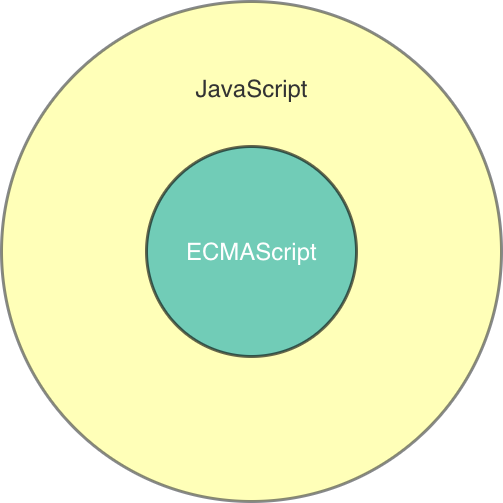
\includegraphics[width=60mm]{./fig/javascript-ecmascript.png}
\caption{JavaScriptとECMAScriptの範囲}
\end{figure}

ECMAScriptの仕様で定義されている機能を学ぶことで、どの実行環境でも対応できる基本的な部分を学べます。
この書籍では、この違いを明確に区別する必要がある場合は「ECMAScript」と「JavaScript」という単語を使い分けます。
そうでない場合、「JavaScript」という単語を使います。

また、このECMAScriptという仕様(共通の部分)も毎年アップデートされ、新しい文法や機能が追加されています。
そのため、実行環境によっては古いバージョンのECMAScriptを実装したものとなっている場合があります。
ECMAScriptは2015年にECMAScript
2015(ES2015)として大きくアップデートされた仕様が公開されました。

今からJavaScriptを学ぶなら、ES2015以降を基本にしたほうがわかりやすいため、この書籍はES2015に基づいた内容となっています。
また、既存のコードはES2015より前のバージョンを元にしたものも多いため、それらのコードに関しても解説しています。

まずは、JavaScript(ECMAScript)とはどのような言語なのかを大まかに見ていきます。

\hypertarget{about-javascript}{%
\section{JavaScriptってどのような言語?}\label{about-javascript}}

JavaScriptは、元々Netscape
Navigatorというブラウザのために開発されたプログラミング言語です。
C、Java、Self、Schemeなどのプログラミング言語の影響を受けて作られました。

JavaScriptは、大部分がオブジェクト(値や処理を1つにまとめたものと考えてください)であり、そのオブジェクト同士のコミュニケーションによって成り立っています。
オブジェクトには、ECMAScriptの仕様として定められたオブジェクト、
実行環境が定義したオブジェクト、ユーザー(つまりあなたです)の定義したオブジェクトが存在します。

この書籍の「\hyperlink{basic-grammar}{第1部 基本文法}」ではECMAScriptの定義する構文やオブジェクトを学んでいきます。
「\hyperlink{use-case}{第2部 ユースケース}」ではブラウザやNode.jsといった実行環境が定義するオブジェクトを学びながら、小さなアプリケーションを作成していきます。
ユーザーの定義したオブジェクトは、コードを書いていくと自然と登場するため、適宜見ていきます。

次に、JavaScriptの言語的な特徴を簡単に紹介していきます。

\hypertarget{case-sensitive}{%
\subsection{大文字と小文字を区別する}\label{case-sensitive}}

まず、JavaScriptは大文字小文字を区別します。
たとえば、次のように\texttt{name}という変数を大文字と小文字で書いた場合に、
それぞれは別々の\texttt{name}と\texttt{NAME}という名前の変数として認識されます。

\begin{lstlisting}
// `name`という名前の変数を宣言
const name = "azu";
// `NAME`という名前の変数を宣言
const NAME = "azu";
\end{lstlisting}

また、大文字で開始しなければならないといった命名規則が意味を持つケースはありません。
そのため、あくまで別々の名前として認識されるというだけになっています
(変数についての詳細は「\href{../variables/README.md}{変数と宣言}」の章で解説します)。

\hypertarget{reserved-keyword}{%
\subsection{予約語を持つ}\label{reserved-keyword}}

JavaScriptには特別な意味を持つキーワードがあり、これらは予約語とも呼ばれます。
このキーワードと同じ名前の変数や関数は宣言できません。
先ほどの、変数を宣言する\texttt{const}も予約語のひとつとなっています。
そのため、\texttt{const}という名前の変数名は宣言できません。

\hypertarget{statement-semicolon}{%
\subsection{文はセミコロンで区切られる}\label{statement-semicolon}}

JavaScriptは、文(Statement)ごとに処理していき、文はセミコロン(\texttt{;})によって区切られます。
特殊なルールに基づき、セミコロンがない文も、行末に自動でセミコロンが挿入されるという仕組みも持っています。\footnote{Automatic
  Semicolon Insertionと呼ばれる仕組みです。}
しかし、暗黙的なものへ頼ると意図しない挙動が発生するため、セミコロンは常に書くようにします
(詳細は「\href{../statement-expression/README.md}{文と式}」の章で解説します)。

また、スペース、タブ文字などは空白文字(ホワイトスペース)と呼ばれます。
これらの空白文字を文にいくつ置いても挙動に違いはありません。

たとえば、次の\texttt{1}足す\texttt{1}を行う2つの文は、\texttt{+}の前後の空白文字の個数に違いはありますが、動作としてはまったく同じ意味となります。

\begin{lstlisting}
// 式や文の間にスペースがいくつあっても同じ意味となる
1 + 1;
1   +   1;
\end{lstlisting}

空白文字の置き方は人によって好みが異なるため、人によって書き方が異なる場合もあります。
複数人で開発する場合は、これらの空白文字の置き方を決めたコーディングスタイルを決めるとよいでしょう。
コーディングスタイルの統一については「\href{../../appendix/links/README.md}{付録:
参考リンク集}」を参照してください。

\hypertarget{strict-mode}{%
\subsection{strict mode}\label{strict-mode}}

JavaScriptには\textbf{strict mode}という実行モードが存在しています。
名前のとおり厳格な実行モードで、古く安全でない構文や機能が一部禁止されています。

\texttt{"use strict"}という文字列をファイルまたは関数の先頭に書くことで、そのスコープにあるコードはstrict
modeで実行されます。
また、後述する``Module''の実行コンテキストでは、このstrict
modeがデフォルトとなっています。

\begin{lstlisting}
"use strict";
// このコードはstrict modeで実行される
\end{lstlisting}

strict
modeでは、\texttt{eval}や\texttt{with}といったレガシーな機能や構文を禁止します。
また、明らかな問題を含んだコードに対しては早期的に例外を投げることで、開発者が間違いに気づきやすくしてくれます。

たとえば、次のような\texttt{const}などのキーワードを含まずに変数を宣言しようとした場合に、strict
modeでは例外が発生します。 strict
modeでない場合は、例外が発生せずにグローバル変数が作られます。

\begin{lstlisting}
"use strict";
mistypedVariable = 42; // => ReferenceError
\end{lstlisting}

このように、strict
modeでは開発者が安全にコードを書けるように、JavaScriptの落とし穴を一部ふさいでくれます。
そのため、常にstrict
modeで実行できるコードを書くことが、より安全なコードにつながります。

本書では、明示的に「strict modeではない」ことを宣言した場合を除き、
すべてstrict modeとして実行できるコードを扱います。

\hypertarget{script-module}{%
\subsection{実行コンテキスト: ScriptとModule}\label{script-module}}

JavaScriptの実行コンテキストとして``Script''と``Module''があります。
コードを書く場合には、この2つの実行コンテキストの違いを意識することは多くありません。

``Script''の実行コンテキストは、多くの実行環境ではデフォルトの実行コンテキストです。
``Script''の実行コンテキストでは、デフォルトはstrict
modeではありません。

``Module''の実行コンテキストは、JavaScriptをモジュールとして実行するために、ECMAScript
2015で導入されたものです。
``Module''の実行コンテキストでは、デフォルトがstrict
modeとなり、古く安全でない構文や機能は一部禁止されています。
また、モジュールの機能は``Module''の実行コンテキストでしか利用できません。モジュールについての詳細は「\href{../../basic/module/README.md}{ECMAScriptモジュール}」の章で解説します。

\hypertarget{ecmascript-updates}{%
\subsection{JavaScriptの仕様は毎年更新される}\label{ecmascript-updates}}

最後に、JavaScriptの仕様であるECMAScriptは毎年更新され、JavaScriptには新しい構文や機能が増え続けています。
そのため、この書籍で学んだ後もまだまだ知らなかったことが出てくるはずです。

一方で、ECMAScriptは後方互換性が慎重に考慮されているため、過去に書いたJavaScriptのコードが動かなくなる変更はほとんど入りません。
そのため、この書籍で学んだことのすべてが無駄になることはありません。

ECMAScriptの仕様がどのように策定されているかについては「\href{../ecmascript/README.md}{ECMAScript}」の章で解説します。

\hypertarget{comment}{%
\chapter{コメント}\label{comment}}

コメントはプログラムとして評価されないため、ソースコードの説明を書くために利用されています。
この書籍でも、JavaScriptのソースコードを解説するためにコメントを使っていきます。

コメントの書き方には、一行コメントと複数行コメントの2種類があります。

\hypertarget{single-line-comment}{%
\section{一行コメント}\label{single-line-comment}}

一行コメントは名前のとおり、一行ずつコメントを書く際に利用します。
\texttt{//}
以降から行末までがコメントとして扱われるため、プログラムとして評価されません。

\begin{lstlisting}
// 一行コメント
// この部分はコードとして評価されない
\end{lstlisting}

\hypertarget{multi-line-comment}{%
\section{複数行コメント}\label{multi-line-comment}}

複数行コメントは名前のとおり、複数行のコメントを書く際に利用します。
一行コメントとは違い複数行をまとめて書けるので、長い説明を書く際に利用されています。

\texttt{/*} と
\texttt{*/}で囲まれた範囲がコメントとして扱われるため、プログラムとして評価されません。

\begin{lstlisting}
/* 
   複数行コメント
   囲まれている範囲がコードとして評価されない
 */
\end{lstlisting}

複数行コメントの中に、複数行コメントを書くことはできません。
次のように、複数行のコメントをネストして書いた場合は構文エラーとなります。

\begin{lstlisting}
/* ネストされた /* 複数行コメント */ は書けない */
\end{lstlisting}

\hypertarget{html-like-comment}{%
\subsection{HTML-likeコメント{$^{\rm ES2015}$}}\label{html-like-comment}}

ECMAScript
2015(ES2015)から後方互換性のための仕様として\textbf{HTML-likeコメント}が追加されています。
このHTML-likeコメントは、ブラウザの実装に合わせた後方互換性のための仕様として定義されています。

HTML-likeコメントは名前のとおり、HTMLのコメントと同じ表記です。

\begin{lstlisting}
<!-- この行はコメントと認識される
console.log("この行はJavaScriptのコードとして実行される");
-->  この行もコメントと認識される
\end{lstlisting}

ここでは、 \texttt{<!--} と
\texttt{-->} がそれぞれ一行コメントとして認識されます。

JavaScriptをサポートしていないブラウザでは、\texttt{<script>}タグを正しく認識できないために書かれたコードが表示されていました。
それを避けるために\texttt{<script>}の中をHTMLコメントで囲み、表示はされないが実行されるという回避策が取られていました。
今は\texttt{<script>}タグをサポートしていないブラウザはないため、この回避策は不要です。

\begin{lstlisting}[language=HTML]
<script language="javascript">
<!--
  document.bgColor = "brown";
// -->
</script>
\end{lstlisting}

一方、\texttt{<script>}タグ内、つまりJavaScript内にHTMLコメントが書かれているサイトは残っています。
このようなサイトでもJavaScriptが動作するという、後方互換性のための仕様として追加されています。

\href{https://dev.mozilla.jp/2016/03/es6-in-depth-arrow-functions/}{歴史的経緯}は別として、ECMAScriptではこのように後方互換性が慎重に取り扱われます。
ECMAScriptは一度入った仕様が使えなくなることはほとんどないため、基本文法で覚えたことが使えなくなることはありません。
一方で、仕様が更新されるたびに新しい機能が増えるため、それを学び続けることには変わりありません。

\hypertarget{conclusion}{%
\section{まとめ}\label{conclusion}}

この章では、ソースコードに説明を書けるコメントについて学びました。

\begin{itemize}
\item
  \texttt{//} 以降から行末までが一行コメント
\item
  \texttt{/*} と
  \texttt{*/}で囲まれた範囲が複数行コメント
\item
  HTML-likeコメントは後方互換性のためだけに存在する
\end{itemize}

\hypertarget{variable-and-declaration}{%
\chapter{変数と宣言}\label{variable-and-declaration}}
\thispagestyle{frontheadings}

プログラミング言語には、文字列や数値などのデータに名前をつけることで、繰り返し利用できるようにする\textbf{変数}という機能があります。

JavaScriptには「これは変数です」という宣言をするキーワードとして、
\texttt{const}、\texttt{let}、\texttt{var}の3つがあります。

\texttt{var}はもっとも古くからある変数宣言のキーワードですが、意図しない動作を作りやすい問題が知られています。
そのためECMAScript
2015で、\texttt{var}の問題を改善するために\texttt{const}と\texttt{let}という新しいキーワードが導入されました。

この章では\texttt{const}、\texttt{let}、\texttt{var}の順に、それぞれの方法で宣言した変数の違いについて見ていきます。

\hypertarget{const}{%
\section[\texttt{const}]{\texttt{const}\protect\icon{fig/es2015.eps}}\label{const}}

\texttt{const}キーワードでは、再代入できない変数の宣言とその変数が参照する値(初期値)を定義できます。

次のように、\texttt{const}キーワードに続いて\texttt{変数名}を書き、代入演算子(\texttt{=})の右辺に変数の\texttt{初期値}を書いて変数を定義できます。

\begin{lstlisting}
const 変数名 = 初期値;
\end{lstlisting}

次のコードでは\texttt{bookTitle}という変数を宣言し、初期値が\texttt{"JavaScript Primer"}という文字列であることを定義しています。

\begin{lstlisting}
const bookTitle = "JavaScript Primer";
\end{lstlisting}

\texttt{const}、\texttt{let}、\texttt{var}どのキーワードも共通の仕組みですが、変数同士を\texttt{,}(カンマ)で区切ることにより、同時に複数の変数を定義できます。

次のコードでは、\texttt{bookTitle}と\texttt{bookCategory}という変数を順番に定義しています。

\begin{lstlisting}
const bookTitle = "JavaScript Primer",
      bookCategory = "プログラミング";
\end{lstlisting}

これは次のように書いた場合と同じ意味になります。

\begin{lstlisting}
const bookTitle = "JavaScript Primer";
const bookCategory = "プログラミング";
\end{lstlisting}

また、\texttt{const}は再代入できない変数を宣言するキーワードです。
そのため、\texttt{const}キーワードで宣言した変数に対して、後から値を代入することはできません。

次のコードでは、\texttt{const}で宣言した変数\texttt{bookTitle}に対して値を再代入しているため、次のようなエラー(\texttt{TypeError})が発生します。
エラーが発生するとそれ以降の処理は実行されなくなります。

\begin{lstlisting}
const bookTitle = "JavaScript Primer";
bookTitle = "新しいタイトル"; // => TypeError: invalid assignment to const
                                  'bookTitle'
\end{lstlisting}

一般的に変数への再代入は「変数の値は最初に定義した値と常に同じである」という参照透過性と呼ばれるルールを壊すため、バグを発生させやすい要因として知られています。そのため、変数に対して値を再代入する必要がない場合は、\texttt{const}キーワードで変数宣言することを推奨しています。

変数に値を再代入したいケースとして、ループなどの反復処理の途中で特定の変数が参照する値を変化させたい場合があります。
そのような場合には、変数への再代入が可能な\texttt{let}キーワードを利用します。

\hypertarget{let}{%
\section[\texttt{let}]{\texttt{let}\protect\icon{fig/es2015.eps}}\label{let}}

\texttt{let}キーワードでは、値の再代入が可能な変数を宣言できます。
\texttt{let}の使い方は\texttt{const}とほとんど同じです。

次のコードでは、\texttt{bookTitle}という変数を宣言し、初期値を\texttt{"JavaScript Primer"}という文字列であることを定義しています。

\begin{lstlisting}
let bookTitle = "JavaScript Primer";
\end{lstlisting}

\texttt{let}は\texttt{const}とは異なり、初期値を指定しない変数も定義できます。
初期値が指定されなかった変数はデフォルト値として\texttt{undefined}という値で初期化されます(\texttt{undefined}は値が未定義ということを表す値です)。

次のコードでは、\texttt{bookTitle}という変数を宣言しています。
このとき\texttt{bookTitle}には初期値が指定されていないため、デフォルト値として\texttt{undefined}で初期化されます。

\begin{lstlisting}
let bookTitle;
// bookTitleは自動的にundefinedという値になる
\end{lstlisting}

この\texttt{let}で宣言された\texttt{bookTitle}という変数には、代入演算子(\texttt{=})を使うことで値を代入できます。
代入演算子(\texttt{=})の右側には変数へ代入する値を書きますが、ここでは\texttt{"JavaScript Primer"}という文字列を代入しています。

\begin{lstlisting}
let bookTitle;
bookTitle = "JavaScript Primer";
\end{lstlisting}

\texttt{let}で宣言した変数に対しては何度でも値の代入が可能です。

\begin{lstlisting}
let count = 0;
count = 1;
count = 2;
count = 3;
\end{lstlisting}

\hypertarget{var}{%
\section{\texorpdfstring{\texttt{var}}{var}}\label{var}}

\texttt{var}キーワードでは、値の再代入が可能な変数を宣言できます。
\texttt{var}の使い方は\texttt{let}とほとんど同じです。

\begin{lstlisting}
var bookTitle = "JavaScript Primer";
\end{lstlisting}

\texttt{var}では、\texttt{let}と同じように初期値がない変数を宣言でき、変数に対して値の再代入もできます。

\begin{lstlisting}
var bookTitle;
bookTitle = "JavaScript Primer";
bookTitle = "新しいタイトル";
\end{lstlisting}

\hypertarget{var-issues}{%
\subsection{\texorpdfstring{\texttt{var}の問題}{varの問題}}\label{var-issues}}

\texttt{var}は\texttt{let}とよく似ていますが、\texttt{var}キーワードには同じ名前の変数を再定義できてしまう問題があります。

\texttt{let}や\texttt{const}では、同じ名前の変数を再定義しようとすると、次のような構文エラー(\texttt{SyntaxError})が発生します。
そのため、間違えて変数を二重に定義してしまうというミスを防ぐことができます。

\begin{lstlisting}
// "x"という変数名で変数を定義する
let x;
// 同じ変数名の変数"x"を定義するとSyntaxErrorとなる
let x; // => SyntaxError: redeclaration of let x
\end{lstlisting}

一方、\texttt{var}は同じ名前の変数を再定義できます。
これは意図せずに同じ変数名で定義してもエラーとならずに、値を上書きしてしまいます。

\begin{lstlisting}
// "x"という変数を定義する
var x = 1;
// 同じ変数名の変数"x"を定義できる
var x = 2;
// 変数xは2となる
\end{lstlisting}

また\texttt{var}には変数の巻き上げと呼ばれる意図しない挙動があり、\texttt{let}や\texttt{const}ではこの問題が解消されています。
\texttt{var}による変数の巻き上げの問題については「\hyperlink{function-and-scope}{関数とスコープ}」の章で解説します。
そのため、現時点では「\texttt{let}は\texttt{var}を改善したバージョン」ということだけ覚えておくとよいです。

このように、\texttt{var}にはさまざまな問題があります。
また、ほとんどすべてのケースで\texttt{var}は\texttt{const}か\texttt{let}に置き換えが可能です。
そのため、これから書くコードに対して\texttt{var}を利用することは避けたほうがよいでしょう。

\begin{tcolorbox}[title=なぜ\texttt{let}や\texttt{const}は追加されたのか?]\label{why-add-let-and-const}

ECMAScript
2015では、\texttt{var}そのものを改善するのではなく、新しく\texttt{const}と\texttt{let}というキーワードを追加することで、\texttt{var}の問題を回避できるようにしました。\texttt{var}自体の動作を変更しなかったのは、後方互換性のためです。

なぜなら、\texttt{var}の挙動自体を変更してしまうと、すでに\texttt{var}で書かれたコードの動作が変わってしまい、動かなくなるアプリケーションが出てくるためです。
新しく\texttt{const}や\texttt{let}などのキーワードをECMAScript仕様に追加しても、そのキーワードを使っているソースコードは追加時点では存在しません\footnote{\texttt{let}や\texttt{const}はECMAScript 2015以前に予約語として定義されていたため、既存のコードと衝突する可能性はありませんでした。}。
そのため、\texttt{const}や\texttt{let}が追加されても後方互換性には影響がありません。

このように、ECMAScriptでは機能を追加する際にも後方互換性を重視しているため、\texttt{var}自体の挙動は変更されませんでした。
\end{tcolorbox}

\hypertarget{variable-name}{%
\section{変数名に使える名前のルール}\label{variable-name}}

ここまで\texttt{const}、\texttt{let}、\texttt{var}での変数宣言とそれぞれの特徴について見てきました。
どのキーワードにおいても宣言できる変数に利用できる名前のルールは同じです。
また、このルールは変数の名前や関数の名前といったJavaScriptの識別子において共通するルールとなります。

変数名の名前(識別子)には、次のルールがあります。

\begin{enumerate}
\def\labelenumi{\arabic{enumi}.}
\item
  半角のアルファベット、\texttt{\_}(アンダースコア)、\texttt{\$}(ダラー)、数字を組み合わせた名前にする
\item
  変数名は数字から開始できない
\item
  予約語と被る名前は利用できない
\end{enumerate}

変数の名前は、半角のアルファベットである\texttt{A}から\texttt{Z}(大文字)と\texttt{a}から\texttt{z}(小文字)、\texttt{\_}(アンダースコア)、\texttt{\$}(ダラー)、数字の\texttt{0}から\texttt{9}を組み合わせた名前にします。JavaScriptでは、アルファベットの大文字と小文字は区別されます。

これらに加えて、ひらがなや一部の漢字なども変数名に利用できますが、全角の文字列が混在すると環境によって扱いにくいこともあるためお勧めしません。

\begin{lstlisting}
var $; // OK: $が利用できる
var _title; // OK: _が利用できる
var jquery; // OK: 小文字のアルファベットが利用できる
var TITLE; // OK: 大文字のアルファベットが利用できる
var es2015; // OK: 数字は先頭以外なら利用できる
var 日本語の変数名; // OK: 一部の漢字や日本語も利用できる
\end{lstlisting}

変数名に数字を含めることはできますが、変数名を数字から開始することはできません。
これは変数名と数値が区別できなくなってしまうためです。

\begin{lstlisting}
var 1st; // NG: 数字から始まっている
var 123; // NG: 数字のみで構成されている
\end{lstlisting}

また、予約語として定義されているキーワードは変数名には利用できません。
予約語とは、\texttt{var}のように構文として意味を持つキーワードのことです。
予約語の一覧は\href{https://developer.mozilla.org/ja/docs/Web/JavaScript/Reference/Reserved_Words}{「予約語 --- JavaScript \textbar{}
MDN」}\footnote{\url{https://developer.mozilla.org/ja/docs/Web/JavaScript/Reference/Reserved_Words}}で確認できますが、基本的には構文として利用される名前が予約されています。

\begin{lstlisting}
var var; // NG: varは変数宣言のために予約されているので利用できない
var if; // NG: ifはif文のために予約されているので利用できない
\end{lstlisting}

\hypertarget{const-is-not-constant}{%
\begin{tcolorbox}[title=\texttt{const}は定数ではない]\label{const-is-not-constant}}

\texttt{const}は「再代入できない変数」を定義する変数宣言であり、必ずしも定数を定義するわけではありません。
定数とは、一度定義した名前(変数名)が常に同じ値を示すものです。

JavaScriptでも、\texttt{const}宣言によって定数に近い変数を定義できます。
次のように、\texttt{const}宣言によって定義した変数を、変更できないプリミティブな値で初期化すれば、それは実質的に定数です。
プリミティブな値とは、数値や文字列などオブジェクト以外のデータです(詳細は「\hyperlink{data-type-and-literal}{データ型とリテラル}」の章で解説します)。

\begin{lstlisting}
// TEN_NUMBERという変数は常に10という値を示す
const TEN_NUMBER = 10;
\end{lstlisting}

しかし、JavaScriptではオブジェクトなども\texttt{const}宣言できます。
次のコードのように、オブジェクトという値そのものは、初期化したあとでも変更できます。

\begin{lstlisting}
// constでオブジェクトを定義している
const object = {
    key: "値"
};
// オブジェクトそのものは変更できてしまう
object.key = "新しい値";
\end{lstlisting}

このように、\texttt{const}で宣言した変数が常に同じ値を示すとは限らないため、定数とは呼べません
(詳細は「\hyperlink{object}{オブジェクト}」の章で解説します)。

また\texttt{const}には、変数名の命名規則はなく、代入できる値にも制限はありません。
そのため、\texttt{const}宣言の特性として「再代入できない変数」を定義すると理解しておくのがよいでしょう。
\end{tcolorbox}

\hypertarget{summary}{%
\section{まとめ}\label{summary}}

この章では、JavaScriptにおける変数宣言を行うキーワードとして\texttt{const}、\texttt{let}、\texttt{var}があることについて学びました。

\begin{itemize}
\item
  \texttt{const}は、再代入できない変数を宣言できる
\item
  \texttt{let}は、再代入ができる変数を宣言できる
\item
  \texttt{var}は、再代入ができる変数を宣言できるが、いくつかの問題が知られている
\item
  変数の名前(識別子)には利用できる名前のルールがある
\end{itemize}

\texttt{var}はほとんどすべてのケースで\texttt{let}や\texttt{const}に置き換えが可能です。
\texttt{const}は再代入できない変数を定義するキーワードです。再代入を禁止することで、ミスから発生するバグを減らすことが期待できます。
このため変数を宣言する場合には、まず\texttt{const}で定義できないかを検討し、できない場合は\texttt{let}を使うことを推奨しています。

\hypertarget{read-eval-print}{%
\chapter{値の評価と表示}\label{read-eval-print}}

変数宣言を使うことで値に名前をつける方法を学びました。
次はその値をどのように評価するかについてです。

値の評価とは、入力した値を評価してその結果を返すことを示しています。
たとえば、次のような値の評価があります。

\begin{itemize}
\item
  \texttt{1 + 1} という式を評価したら
  \texttt{2} という結果を返す
\item
  \texttt{bookTitle}
  という変数を評価したら、変数に代入されている値を返す
\item
  \texttt{const x = 1;}という文を評価することで変数を定義するが、この文には返り値はありません
\end{itemize}

この値の評価方法を確認するために、ウェブブラウザ(以下ブラウザ)を使ってJavaScriptを実行する方法を見ていきます。

\hypertarget{recommended-browser}{%
\section{この書籍で利用するブラウザ}\label{recommended-browser}}

まずはブラウザ上でJavaScriptのコードを実行してみましょう。
この書籍ではブラウザとして\href{https://www.mozilla.org/ja/firefox/}{Firefox}を利用します。
次のURLからFirefoxをダウンロードし、インストールしてください。

\begin{itemize}
\item
  Firefox: \url{https://www.mozilla.org/ja/firefox/}
\end{itemize}

この書籍で紹介するサンプルコードのほとんどは、Google Chrome、Microsoft
Edge、Safariなどのブラウザの最新版でも動作します。
一方で、古いJavaScriptしかサポートしていないInternet
Explorerでは多くのコードは動作しません。

また、ブラウザによっては標準化されていないエラーメッセージの細かな違いや開発者ツールの使い方の違いなどもあります。
この書籍ではFirefoxで実行した結果を記載しています。
そのため、Firefox以外のブラウザでは細かな違いがあることに注意してください。

\hypertarget{execute-js-on-browser}{%
\section{ブラウザでJavaScriptを実行する}\label{execute-js-on-browser}}

ブラウザでJavaScriptを実行する方法としては大きく分けて2つあります。
1つ目はブラウザの開発者ツールのコンソール上でJavaScriptコードを評価する方法です。
2つ目はHTMLファイルを作成しJavaScriptコードを読み込む方法です。

\hypertarget{repl-on-browser}{%
\subsection{ブラウザの開発者ツールのコンソール上でJavaScriptコードを評価する方法}\label{repl-on-browser}}

ブラウザやNode.jsなど多くの実行環境には、コードを評価してその結果を表示するREPL(read--eval--print
loop)と呼ばれる開発者向けの機能があります。
Firefoxでは、開発者ツールの\textbf{Webコンソール}と呼ばれるパネルにREPL機能が含まれています。
REPL機能を使うことで、試したいコードをその場で実行できるため、JavaScriptの動作を理解するのに役立ちます。

REPL機能を使うには、まずFirefoxの開発者ツールを次のいずれかの方法で開きます。

\begin{itemize}
\item
  Firefox メニュー(メニューバーがある場合や macOS
  では、ツールメニュー)の Web 開発サブメニューで ``Web コンソール''
  を選択する
\item
  キーボードショートカット Ctrl+Shift+K(macOS では
  Command+Option+K)を押下する
\end{itemize}

詳細は``\href{https://developer.mozilla.org/ja/docs/Tools/Web_Console/Opening_the_Web_Console}{Webコンソールを開く}''を参照してください。

\begin{figure}
\centering
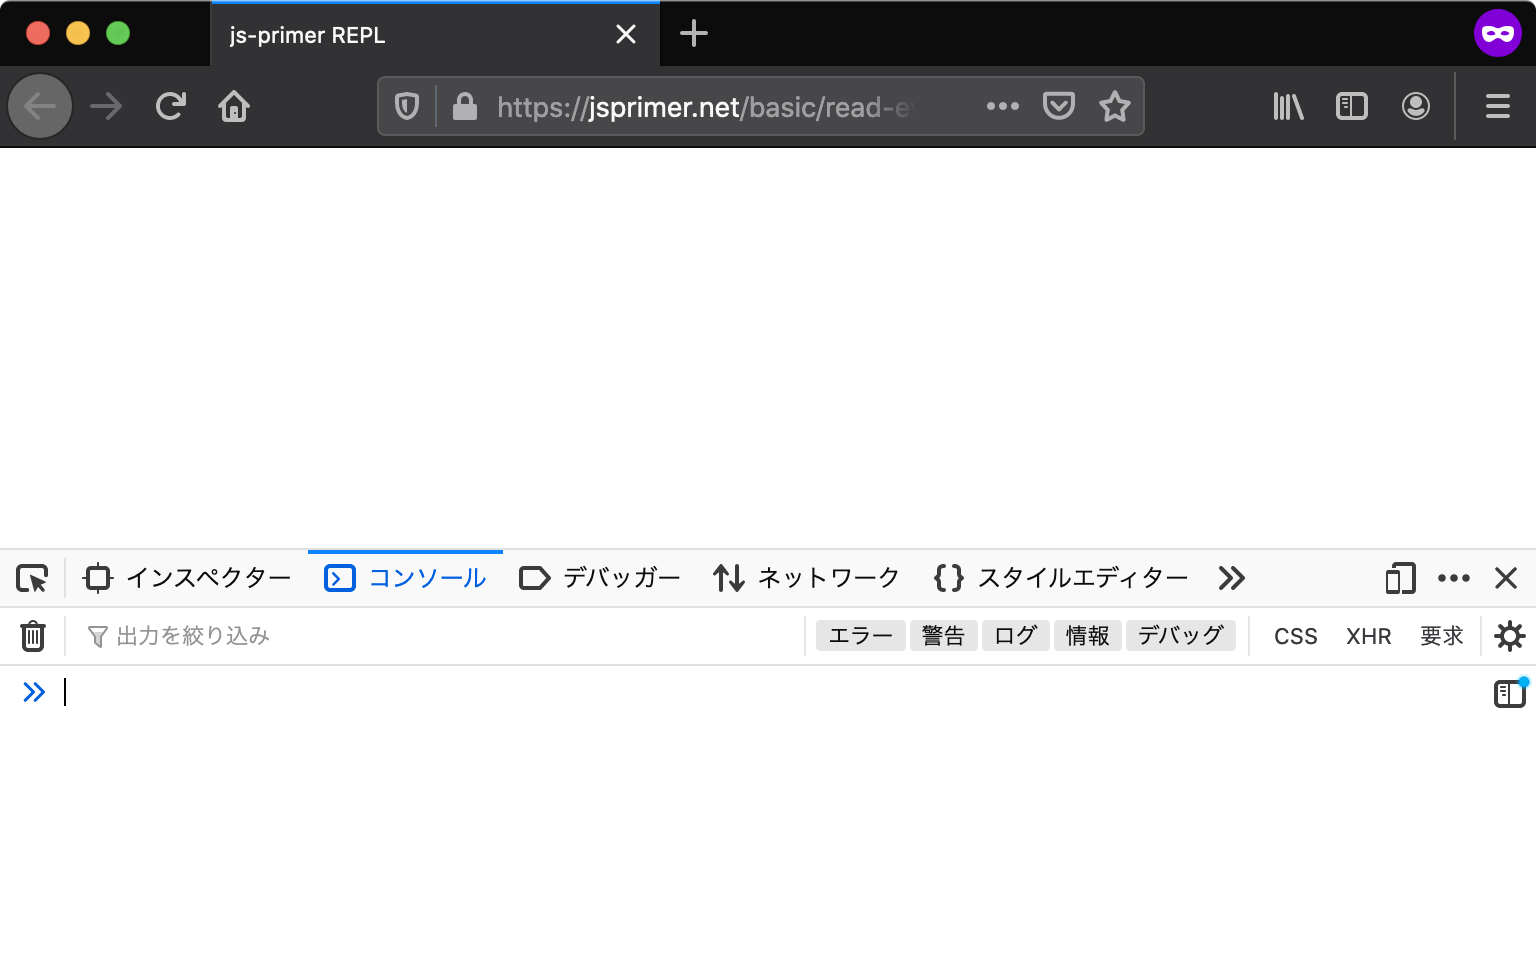
\includegraphics[width=100mm]{./fig/web-console.png}
\caption{FirefoxでWebコンソールを開いた状態}
\end{figure}

開発者ツールの``コンソール''タブを選択すると、コマンドライン(二重山カッコ\texttt{>>}からはじまる欄)に任意のコードを入力し評価できます。
このコマンドラインがブラウザにおけるREPL機能です。

REPLに\texttt{1}という値を入力すると、その評価結果である\texttt{1}が次の行に表示されます。

\begin{lstlisting}
>> 1
1
\end{lstlisting}

\texttt{1 + 1}
という式を入力すると、その評価結果である\texttt{2}が次の行に表示されます。

\begin{lstlisting}
>> 1 + 1
2
\end{lstlisting}

次に\texttt{const}キーワードを使って\texttt{bookTitle}という変数を宣言してみると、\texttt{undefined}という結果が次の行に表示されます。
変数宣言は変数名と値を関連づけるだけであるため、変数宣言自体は何も値を返さないという意味で\texttt{undefined}が結果になります。
REPLではそのまま次の入力ができるため、\texttt{bookTitle}という入力をすると、先ほど変数に入れた\texttt{"JavaScriptの本"}という結果が次の行に表示されます。

\begin{lstlisting}
>> const bookTitle = "JavaScriptの本";
undefined
>> bookTitle
"JavaScriptの本"
\end{lstlisting}

このようにコマンドラインのREPL機能では、JavaScriptのコードを1行ごとに実行できます。
Shift + Enterで改行して複数行の入力もできます。
好きな単位でJavaScriptのコードを評価できるため、コードの動きを簡単に試したい場合などに利用できます。

注意点としては、REPLではそのREPLを終了するまで\texttt{const}キーワードなどで宣言した変数が残り続けます。
たとえば、\texttt{const}での変数宣言は同じ変数名を二度定義できないというルールでした。
そのため1行ずつ実行しても、同じ変数名を定義したことになるため構文エラー(\texttt{SyntaxError})となります。

\begin{lstlisting}
>> const bookTitle = "JavaScriptの本";
undefined
>> const bookTitle = "JavaScriptの本";
SyntaxError: redeclaration of const bookTitle
\end{lstlisting}

ブラウザでは、開発者ツールを開いているウェブページでリロードするとREPLの実行状態もリセットされます。
\texttt{redeclaration}(再定義)に関するエラーメッセージが出た際にはページをリロードしてみてください。

\hypertarget{js-in-html}{%
\subsection{HTMLファイルを作成しJavaScriptコードを読み込む方法}\label{js-in-html}}

REPLはあくまで開発者向けの機能です
ウェブサイトではHTMLに記述した\texttt{<script>}タグでJavaScriptを読み込み実行します。
ここでは、HTMLとJavaScriptファイルを使ったJavaScriptコードの実行方法を見ていきます。

HTMLファイルとJavaScriptファイルの2種類を使い、JavaScriptのコードを実行する準備をしていきます。
ファイルを作成するため\href{https://atom.io/}{Atom}や\href{https://code.visualstudio.com/}{Visual
Studio
Code}などのJavaScriptに対応したエディターを用意しておくとスムーズです。
エディターはどんなものでも問題ありませんが、必ず文字コード(エンコーディング)は\textbf{UTF-8}、改行コードは\textbf{LF}にしてファイルを保存してください。

ファイルを作成するディレクトリはどんな場所でも問題ありませんが、ここでは\texttt{example}という名前のディレクトリにファイルを作成していきます。

まずはJavaScriptファイルとして\texttt{index.js}ファイルを\texttt{example/index.js}というパスに作成します。
\texttt{index.js}の中には次のようなコードを書いておきます。

\begin{listtitle}
index.js
\end{listtitle}
\begin{lstlisting}
1;
\end{lstlisting}
\listend

次にHTMLファイルとして\texttt{index.html}ファイルを\texttt{example/index.html}というパスに作成します。
このHTMLファイルから先ほど作成した\texttt{index.js}ファイルを読み込み実行します。
\texttt{index.html}の中には次のようなコードを書いておきます。

\begin{listtitle}
index.html
\end{listtitle}
\begin{lstlisting}
<html>
<head>
    <meta charset="UTF-8">
    <title>Example</title>
    <script src="./index.js"></script>
</head>
<body></body>
</html>
\end{lstlisting}
\listend

重要なのは\texttt{<script src="./index.js"></script>}という記述です。
これは同じディレクトリにある\texttt{index.js}という名前のJavaScriptファイルをスクリプトとして読み込むという意味になります。

最後にブラウザで作成した\texttt{index.html}を開きます。
HTMLファイルを開くには、ブラウザにHTMLファイルをドラッグアンドドロップするかまたはファイルメニューから``ファイルを開く''でHTMLファイルを選択します。
HTMLファイルを開いた際に、ブラウザのアドレスバーには\texttt{file:///}からはじまるローカルファイルのファイルパスが表示されます。

先ほどと同じ手順で``Web
コンソール''を開いてみると、コンソールには何も表示されていないはずです。
REPLでは自動で評価結果のコンソール表示まで行いますが、JavaScriptコードとして読み込んだ場合は勝手に評価結果を表示することはありません。
あくまで自動表示はREPLの機能です。そのため多くの実行環境では\textbf{コンソール表示}するためのAPI(機能)が存在しています。

\hypertarget{console-api}{%
\section{Console API}\label{console-api}}

JavaScriptの多くの実行環境では、Console
APIを使って\textbf{コンソールに表示}します。
\texttt{console.log(引数)}の引数にコンソール表示したい値を渡すことで、評価結果がコンソールに表示されます。

先ほどの\texttt{index.js}の中身を次のように書き換えます。
そしてページをリロードすると、 \texttt{1}
という値を評価した結果がWebコンソールに表示されます。

\begin{listtitle}
index.js
\end{listtitle}
\begin{lstlisting}
console.log(1); // => 1
\end{lstlisting}
\listend

次のように引数に式を書いた場合は先に引数(\texttt{(}と\texttt{)}の間に書かれたもの)の式を評価してから、その結果をコンソールに表示します。
そのため、\texttt{1 + 1} の評価結果として
\texttt{2} がコンソールに表示されます。

\begin{listtitle}
index.js
\end{listtitle}
\begin{lstlisting}
console.log(1 + 1); // => 2
\end{lstlisting}
\listend

同じように引数に変数を渡すこともできます。
この場合もまず先に引数である変数を評価してから、その結果をコンソールに表示します。

\begin{listtitle}
index.js
\end{listtitle}
\begin{lstlisting}
const total = 42 + 42;
console.log(total); // => 84
\end{lstlisting}
\listend

Console APIは原始的なプリントデバッグとして利用できます。
「この値は何だろう」と思ったらコンソールに表示すると解決する問題は多いです。
またJavaScriptの開発環境は高機能化が進んでいるため、Console
API以外にもさまざまな機能がありますがここでは詳細は省きます。

この書籍では、コード内で評価結果を表示するためにConsole
APIを利用していきます。

すでに何度も登場していますが、コード内のコメントで\texttt{// => 評価結果}と書いている場合があります。
このコメントは、その左辺にある値を評価した結果またはConsole
APIで表示した結果を掲載しています。

\begin{lstlisting}
// 式の評価結果の例(コンソールには表示されない)
1; // => 1
const total = 42 + 42;
// 変数の評価結果の例(コンソールには表示されない)
total; // => 84
// Console APIでコンソールに表示する例
console.log("JavaScript"); // => "JavaScript"
\end{lstlisting}

\hypertarget{execute-on-web}{%
\section{ウェブ版の書籍でコードを実行する}\label{execute-on-web}}

ウェブ版の書籍では実行できるサンプルコードには\textbf{実行}というボタンが配置されています。
このボタンでは実行するたびに毎回新しい環境を作成して実行するため、REPLで発生する変数の再定義といった問題はおきません。

一方で、REPLと同じように\texttt{1}というコードを実行すると\texttt{1}という評価結果を得られます。
またConsole
APIにも対応しています。サンプルコードを改変して実行するなど、よりコードへの理解を深めるために利用できます。

\begin{lstlisting}
console.log("Console APIで表示");
// 値を評価した場合は最後の結果が表示される
42; // => 42
\end{lstlisting}

\hypertarget{eval-code-and-error}{%
\section{コードの評価とエラー}\label{eval-code-and-error}}

JavaScriptのコードを実行したときにエラーメッセージが表示されて意図したように動かなかった場合もあるはずです。
プログラムを書くときに一度もエラーを出さずに書き終えることはほとんどありません。
特に新しいプログラミング言語を学ぶ際にはトライアンドエラー(試行錯誤)することはとても重要です。

エラーメッセージがWebコンソールに表示された際には、あわてずにそのエラーメッセージを読むことで多くの問題は解決できます。
またエラーには多く分けて構文エラーと実行時エラーの2種類があります。
ここではエラーメッセージの簡単な読み方を知り、そのエラーを修正する足がかりを見ていきます。

\hypertarget{syntax-error}{%
\subsection{構文エラー}\label{syntax-error}}

構文エラーは書かれたコードの文法が間違っている場合に発生するエラーです。

JavaScriptエンジンは、コードをパース(解釈)してから、プログラムとして実行できる形に変換して実行します。
コードをパースする際に文法の問題が見つかると、その時点で構文エラーが発生するためプログラムとして実行できません。

次のコードでは、関数呼び出しに\texttt{)}をつけ忘れているため構文エラーが発生します。

\begin{listtitle}
index.js
\end{listtitle}
\begin{lstlisting}
console.log(1; // => SyntaxError: missing ) after argument list
\end{lstlisting}
\listend

\begin{figure}
\centering
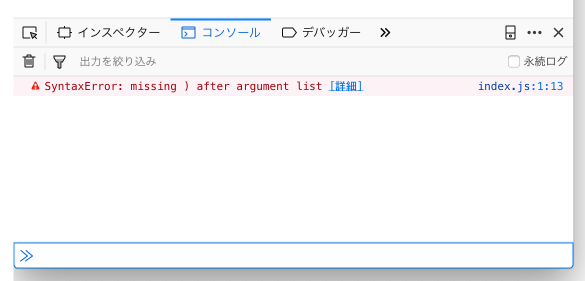
\includegraphics{./fig/syntax-error.png}
\caption{SyntaxError in Console}
\end{figure}

Firefoxでこのコードを実行すると次のようなエラーメッセージがコンソールに表示されます。

\begin{quote}
SyntaxError: missing ) after argument list{[}詳細{]} index.js:1:13
\end{quote}

エラーメッセージはブラウザによって多少の違いはありますが、基本的には同じ形式のメッセージになります。
このエラーメッセージをパーツごとに見てみると次のようになります。

\begin{lstlisting}
SyntaxError: missing ) after argument list[詳細] index.js:1:13 
^^^^^^^^^^^  ^^^^^^^^^^^^^^^^^^^^^^^^^^^^^      ^^^^^^^^ ^^^^
エラーの種類                |                        |  行番号:列番号
                  エラー内容の説明                 ファイル名
\end{lstlisting}

\begin{longtable}[]{@{}ll@{}}
\toprule
\begin{minipage}[b]{0.47\columnwidth}\raggedright
メッセージ\strut
\end{minipage} & \begin{minipage}[b]{0.47\columnwidth}\raggedright
意味\strut
\end{minipage}\tabularnewline
\midrule
\endhead
\begin{minipage}[t]{0.47\columnwidth}\raggedright
\texttt{SyntaxError: missing ) after argument list}\strut
\end{minipage} & \begin{minipage}[t]{0.47\columnwidth}\raggedright
エラーの種類は\texttt{SyntaxError}で、関数呼び出しの\texttt{)}が足りないこと\strut
\end{minipage}\tabularnewline
\begin{minipage}[t]{0.47\columnwidth}\raggedright
\texttt{index.js:1:13}\strut
\end{minipage} & \begin{minipage}[t]{0.47\columnwidth}\raggedright
例外が\texttt{index.js}の1行目13列目で発生したこと\strut
\end{minipage}\tabularnewline
\bottomrule
\end{longtable}

Firefoxでは\textbf{{[}詳細{]}}というリンクがエラーメッセージによっては表示されます。
この\textbf{{[}詳細{]}}リンクはエラーメッセージに関するMDNの解説ページへのリンクとなっています。
この例のエラーメッセージでは次の解説ページへリンクされています。

\begin{itemize}
\item
  \url{https://developer.mozilla.org/ja/docs/Web/JavaScript/Reference/Errors/Missing_parenthesis_after_argument_list}
\end{itemize}

このエラーメッセージや解説ページから、関数呼び出しの\texttt{)}が足りないため構文エラーとなっていることがわかります。
そのため、次のように足りない\texttt{)}を追加することでエラーを修正できます。

\begin{lstlisting}
console.log(1);
\end{lstlisting}

構文エラーによっては少しエラーメッセージから意味が読み取りにくいものもあります。

次のコードでは、\texttt{const}を\texttt{cosnt}とタイプミスしているため構文エラーが発生しています。

\begin{listtitle}
index.js
\end{listtitle}
\begin{lstlisting}
cosnt a = 1;
\end{lstlisting}
\listend

\begin{quote}
SyntaxError: unexpected token: identifier{[}詳細{]} index.js:1:6
\end{quote}

\begin{longtable}[]{@{}ll@{}}
\toprule
\begin{minipage}[b]{0.47\columnwidth}\raggedright
メッセージ\strut
\end{minipage} & \begin{minipage}[b]{0.47\columnwidth}\raggedright
意味\strut
\end{minipage}\tabularnewline
\midrule
\endhead
\begin{minipage}[t]{0.47\columnwidth}\raggedright
\texttt{SyntaxError: unexpected token: identifier}\strut
\end{minipage} & \begin{minipage}[t]{0.47\columnwidth}\raggedright
エラーの種類は\texttt{SyntaxError}で、予期しないものが識別子(変数名)に指定されている\strut
\end{minipage}\tabularnewline
\begin{minipage}[t]{0.47\columnwidth}\raggedright
\texttt{index.js:1:6}\strut
\end{minipage} & \begin{minipage}[t]{0.47\columnwidth}\raggedright
例外が\texttt{index.js}の1行目6列目で発生したこと\strut
\end{minipage}\tabularnewline
\bottomrule
\end{longtable}

プログラムをパースする際に\texttt{index.js:1:6}で予期しない(構文として解釈できない)識別子が見つかったため、構文エラーが発生したという意味になります。
1行目6列目(行は1から、列は0からカウントする)である\texttt{a}という文字列がおかしいということになります。
しかし、実際には\texttt{cosnt}というタイプミスがこの構文エラーの原因です。

なぜこのようなエラーメッセージになるかというと、\texttt{cosnt}(\texttt{const}のタイプミス)はキーワードではないため、ただの変数名として解釈されます。
そのため、このコードは次のようなコードであると解釈され、そのような文法は認められないということで構文エラーとなっています。

\begin{lstlisting}
cosntという変数名 aという変数名 = 1;
\end{lstlisting}

このようにエラーメッセージとエラーの原因は必ずしも一致しません。
しかし、構文エラーの原因はコードの書き間違いであることがほとんどです。
そのため、エラーが発生した位置やその周辺を注意深く見ることで、エラーの原因を特定できます。

\hypertarget{runtime-error}{%
\subsection{実行時エラー}\label{runtime-error}}

実行時エラーはプログラムを実行している最中に発生するエラーです。
実行時(ランタイム)におきるエラーであるため、ランタイムエラーと呼ばれることもあります。
APIに渡す値の問題から起きる\texttt{TypeError}や存在しない変数を参照しようとして起きる\texttt{ReferenceError}などさまざまな種類があります。

実行時エラーが発生した場合は、そのコードは構文としては正しい(構文エラーではない)のですが、別のことが原因でエラーが発生しています。

次のコードでは\texttt{x}という存在しない変数を参照したため、\texttt{ReferenceError}という実行時エラーが発生しています。

\begin{listtitle}
index.js
\end{listtitle}
\begin{lstlisting}
const value = "値";
console.log(x); // => ReferenceError: x is not defined
\end{lstlisting}
\listend

\begin{quote}
ReferenceError: x is not defined{[}詳細{]} index.js:2:1
\end{quote}

\begin{longtable}[]{@{}ll@{}}
\toprule
\begin{minipage}[b]{0.47\columnwidth}\raggedright
メッセージ\strut
\end{minipage} & \begin{minipage}[b]{0.47\columnwidth}\raggedright
意味\strut
\end{minipage}\tabularnewline
\midrule
\endhead
\begin{minipage}[t]{0.47\columnwidth}\raggedright
\texttt{ReferenceError: x is not defined}\strut
\end{minipage} & \begin{minipage}[t]{0.47\columnwidth}\raggedright
エラーの種類は\texttt{ReferenceError}で、\texttt{x}という未定義の識別子を参照したため発生\strut
\end{minipage}\tabularnewline
\begin{minipage}[t]{0.47\columnwidth}\raggedright
\texttt{index.js:2:1}\strut
\end{minipage} & \begin{minipage}[t]{0.47\columnwidth}\raggedright
例外が\texttt{index.js}の2行目1列目で発生したこと\strut
\end{minipage}\tabularnewline
\bottomrule
\end{longtable}

\texttt{x}という変数や関数が存在するかは、実行してみないとわかりません。
そのため、実行して\texttt{x}という識別子を参照したときに、初めて\texttt{x}が存在するかが判明し、\texttt{x}が存在しない場合は\texttt{ReferenceError}となります。

この例では、\texttt{value}変数を参照しているつもりで、\texttt{x}という存在しない変数を参照していたのが原因のようです。
先ほどのコードは、次のように参照する変数を\texttt{value}に変更すれば、エラーが修正できます。

\begin{lstlisting}
const value = "値";
console.log(value); // => "値"
\end{lstlisting}

このように、実行時エラーは該当する箇所を実行するまで、エラーになるかがわからない場合も多いのです。
そのため、どこまではちゃんと実行できたか順番に追っていくような、エラーの原因を特定する作業が必要になる場合があります。
このようなエラーの原因を特定し、修正する作業のことを\textbf{デバッグ}と呼びます。

実行時エラーは構文エラーに比べてエラーの種類も多く、その原因もプログラムの数だけあります。
そのため、エラーの原因を見つけることが大変な場合もあります。
しかし、JavaScriptはとてもよく使われている言語なので、ウェブ上には類似するエラーを報告している人も多いです。
エラーメッセージで検索をしてみると、類似するエラーの原因と解消方法が見つかるケースもあります。

実行時エラーが発生した際には、発生したエラーの行数の周辺をよく見ることやエラーメッセージを調べてみることが大切です。

\hypertarget{conclusion}{%
\section{まとめ}\label{conclusion}}

ブラウザ上でJavaScriptを実行する方法として開発者ツールを使う方法とHTMLからJavaScriptファイルを読み込む方法を紹介しました。
「第一部
基本文法」で紹介するサンプルコードは基本的にこれらの方法で実行できます。
サンプルコードを自分なりに改変して実行してみるとより理解が深くなるため、サンプルコードの動作を自分自身で確認してみてください。

コードを実行してエラーが発生した場合にはエラーメッセージや位置情報などが表示されます。
これらのエラー情報を使ってデバッグすることでエラーの原因を取り除けるはずです。

JavaScriptにおいては多くのエラーはすでに類似するケースがウェブ上に報告されています。
構文エラーや実行時エラーの典型的なものはMDNの\href{https://developer.mozilla.org/ja/docs/Web/JavaScript/Reference/Errors}{JavaScript
エラーリファレンス}にまとめられています。
また\href{https://www.google.com/}{Google}、\href{https://github.com/}{GitHub}、\href{https://stackoverflow.com/}{Stack
Overflow}などでエラーメッセージを検索することで、エラーの原因を見つけられることもあります。

エラーがWebコンソールに表示されているならば、そのエラーは修正できます。
エラーを過度に怖がる必要はありません。エラーメッセージなどのヒントを使ってエラーを修正していけるようにしましょう。

\hypertarget{data-type-and-literal}{%
\chapter{データ型とリテラル}\label{data-type-and-literal}}
\thispagestyle{frontheadings}

\hypertarget{data-type}{%
\section{データ型}\label{data-type}}

JavaScriptは動的型づけ言語に分類される言語であるため、静的型づけ言語のような\textbf{\textgt{変数の型}}はありません。
しかし、文字列、数値、真偽値といった\textbf{\textgt{値の型}}は存在します。
これらの値の型のことを\textbf{\textgt{データ型}}と呼びます。

データ型を大きく分けると、\textbf{\textgt{プリミティブ型}}と\textbf{\textgt{オブジェクト}}の2つに分類されます。

プリミティブ型(基本型)は、真偽値や数値などの基本的な値の型のことです。
プリミティブ型の値は、一度作成したらその値自体を変更できないというイミュータブル(immutable)の特性を持ちます。
JavaScriptでは、文字列も一度作成したら変更できないイミュータブルの特性を持ち、プリミティブ型の一種として扱われます。

一方、プリミティブ型ではないものをオブジェクト(複合型)と呼び、
オブジェクトは複数のプリミティブ型の値またはオブジェクトからなる集合です。
オブジェクトは、一度作成した後もその値自体を変更できるためミュータブル(mutable)の特性を持ちます。
オブジェクトは、値そのものではなく値への参照を経由して操作されるため、参照型のデータとも言います。

データ型を細かく見ていくと、6つのプリミティブ型とオブジェクトからなります。

\begin{itemize}
\item
  プリミティブ型(基本型)

  \begin{itemize}
  \item
    真偽値(Boolean):
    \texttt{true}または\texttt{false}のデータ型
  \item
    数値(Number): \texttt{42} や
    \texttt{3.14159} などの数値のデータ型
  \item
    文字列(String): \texttt{"JavaScript"}
    などの文字列のデータ型
  \item
    undefined: 値が未定義であることを意味するデータ型
  \item
    null: 値が存在しないことを意味するデータ型
  \item
    シンボル(Symbol): ES2015から追加された一意で不変な値のデータ型
  \end{itemize}
\item
  オブジェクト(複合型)

  \begin{itemize}
  \item
    プリミティブ型以外のデータ
  \item
    オブジェクト、配列、関数、正規表現、Dateなど
  \end{itemize}
\end{itemize}

プリミティブ型でないものは、オブジェクトであると覚えていれば問題ありません。

\texttt{typeof}演算子を使うことで、次のようにデータ型を調べることができます。

\begin{lstlisting}
console.log(typeof true);// => "boolean"
console.log(typeof 42); // => "number"
console.log(typeof "JavaScript"); // => "string"
console.log(typeof Symbol("シンボル"));// => "symbol"
console.log(typeof undefined); // => "undefined"
console.log(typeof null); // => "object"
console.log(typeof ["配列"]); // => "object"
console.log(typeof { "key": "value" }); // => "object"
console.log(typeof function() {}); // => "function"
\end{lstlisting}

残念ながら\texttt{typeof null}が\texttt{"object"}となるのは、歴史的経緯のある仕様のバグ\footnote{JavaScriptが最初にNetscapeで実装された際に\texttt{typeof null === "object"}となるバグがありました。このバグを修正するとすでにこの挙動に依存しているコードが壊れるため、修正が見送られ現在の挙動が仕様となりました。詳しくは\url{https://2ality.com/2013/10/typeof-null.html}を参照。}です。
他のプリミティブ型の値については、\texttt{typeof}演算子でそれぞれのデータ型を調べることができます。

一方で、配列とオブジェクトがどちらも\texttt{"object"}という判定結果になります。
このように、\texttt{typeof}演算子ではすべてのオブジェクトの種類を判定することはできません。

基本的に\texttt{typeof}演算子は、プリミティブ型またはオブジェクトかを判別するものです。
オブジェクトの詳細な種類を判定できないことは、覚えておくとよいでしょう。
各オブジェクトの判定方法については、それぞれのオブジェクトの章で見ていきます。

\hypertarget{literal}{%
\section{リテラル}\label{literal}}

プリミティブ型の値や一部のオブジェクトは、\textbf{リテラル}を使うことで簡単に定義できるようになっています。

リテラルとはプログラム上で数値や文字列など、データ型の値を直接記述できるように構文として定義されたものです。
たとえば、\texttt{"}と\texttt{"}で囲んだ範囲が文字列リテラルで、これは文字列型のデータを表現しています。

次のコードでは、\texttt{"こんにちは"}という文字列型のデータを初期値に持つ変数\texttt{str}を定義しています。

\begin{lstlisting}
// "と"で囲んだ範囲が文字列リテラル
const str = "こんにちは";
\end{lstlisting}

リテラル表現がない場合は、その値を作る関数に引数を渡して作成する形になります。
そのような冗長な表現を避ける方法として、よく利用される主要な値にはリテラルが用意されています。

次の4つのプリミティブ型は、それぞれリテラル表現を持っています。

\begin{itemize}
\item
  真偽値
\item
  数値
\item
  文字列
\item
  null
\end{itemize}

また、オブジェクトの中でもよく利用されるものに関してはリテラル表現が用意されています。

\begin{itemize}
\item
  オブジェクト
\item
  配列
\item
  正規表現
\end{itemize}

これらのリテラルについて、まずはプリミティブ型から順番に見ていきます。

\hypertarget{boolean}{%
\subsection{真偽値(Boolean)}\label{boolean}}

真偽値には\texttt{true}と\texttt{false}のリテラルがあります。
それぞれは\texttt{true}と\texttt{false}の値を返すリテラルで、見た目どおりの意味となります。

\begin{lstlisting}
true; // => true
false; // => false
\end{lstlisting}

\hypertarget{number}{%
\subsection{数値(Number)}\label{number}}

数値には大きく分けて\texttt{42}のような整数リテラルと\texttt{3.14159}のような浮動小数点数リテラルがあります。

\hypertarget{integer-literal}{%
\subsubsection{整数リテラル}\label{integer-literal}}

整数リテラルには次の4種類があります。

\begin{itemize}
\item
  10進数: 数字の組み合わせ

  \begin{itemize}
  \item
    ただし、複数の数字を組み合わせた際に、先頭を\texttt{0}から開始すると8進数として扱われる場合があります
  \item
    例)\texttt{0}、\texttt{2}、\texttt{10}
  \end{itemize}
\item
  2進数:
  \texttt{0b}(または\texttt{0B})の後ろに、\texttt{0}または\texttt{1}の数字の組み合わせ

  \begin{itemize}
  \item
    例)\texttt{0b0}、\texttt{0b10}、\texttt{0b1010}
  \end{itemize}
\item
  8進数:
  \texttt{0o}(または\texttt{0O})の後ろに、\texttt{0}から\texttt{7}までの数字の組み合わせ

  \begin{itemize}
  \item
    \texttt{0o}
    は数字のゼロと小文字アルファベットの\texttt{o}
  \item
    例)\texttt{0o644}、\texttt{0o777}
  \end{itemize}
\item
  16進数:
  \texttt{0x}(または\texttt{0X})の後ろに、\texttt{0}から\texttt{9}までの数字と\texttt{a}から\texttt{f}または\texttt{A}から\texttt{F}のアルファベットの組み合わせ

  \begin{itemize}
  \item
    アルファベットの大文字・小文字の違いは値には影響しません
  \item
    例)\texttt{0x30A2}、\texttt{0xEEFF}
  \end{itemize}
\end{itemize}

0から9の数字のみで書かれた数値は、10進数として扱われます。

\begin{lstlisting}
console.log(1); // => 1
console.log(10); // => 10
console.log(255); // => 255
\end{lstlisting}

\texttt{0b}からはじまる2進数リテラルは、ビットを表現するのによく利用されています。
\texttt{b}は2進数を表すbinaryを意味しています。

\begin{lstlisting}
console.log(0b1111); // => 15
console.log(0b10000000000); // => 1024
\end{lstlisting}

\texttt{0o}からはじまる8進数リテラルは、ファイルのパーミッションを表現するのによく利用されています。
\texttt{o}は8進数を表すoctalを意味しています。

\begin{lstlisting}
console.log(0o644);  // => 420
console.log(0o777);  // => 511
\end{lstlisting}

次のように、\texttt{0}からはじまり、\texttt{0}から\texttt{7}の数字を組み合わせた場合も8進数として扱われます。
しかし、この表記は10進数と紛らわしいものであったため、ES2015で\texttt{0o}の8進数リテラルが新たに導入されました。
また、strict
modeではこの書き方は例外が発生するため、次のような8進数の書き方は避けるべきです。

\begin{lstlisting}
// 非推奨な8進数の書き方
// strict modeは例外が発生
console.log(0644);  // => 420
console.log(0777);  // => 511
\end{lstlisting}

\texttt{0x}からはじまる16進数リテラルは、文字のコードポイントやRGB値の表現などに利用されています。
\texttt{x}は16進数を表すhexを意味しています。

\begin{lstlisting}
console.log(0xFF); // => 255
// 小文字で書いても意味は同じ
console.log(0xff); // => 255
console.log(0x30A2); // => 12450
\end{lstlisting}

\begin{small}
\begin{longtable}[l]{p{40mm}|p{40mm}|p{60mm}}
\hline\rowcolor[gray]{0.85}\rule[0mm]{0mm}{4mm}
{\textgt 名前} & {\textgt 表記例} & {\textgt 用途}\tabularnewline
\hline
\endhead
10進数 & 42 & 数値\tabularnewline
2進数 & 0b0001 & ビット演算など\tabularnewline
8進数 & 0o777 & ファイルのパーミッションなど\tabularnewline
16進数 & 0xEEFF & 文字のコードポイント、RGB値など\tabularnewline
\hline
\end{longtable}
\end{small}

\hypertarget{floating-point-number-literal}{%
\subsubsection{浮動小数点数リテラル}\label{floating-point-number-literal}}

JavaScriptの浮動小数点数は\href{https://ja.wikipedia.org/wiki/IEEE_754}{IEEE 754}\footnote{\url{https://ja.wikipedia.org/wiki/IEEE_754}}を採用しています。
浮動小数点数をリテラルとして書く場合には、次の2種類の表記が利用できます。

\begin{itemize}
\item
  \texttt{3.14159} のような
  \texttt{.}(ドット)を含んだ数値
\item
  \texttt{2e8} のような \texttt{e}
  または \texttt{E} を含んだ数値
\end{itemize}

\texttt{0}からはじまる浮動小数点数は、\texttt{0}を省略して書くことができます。

\begin{lstlisting}
.123; // => 0.123
\end{lstlisting}

しかし、JavaScriptでは\texttt{.}をオブジェクトにおいて利用する機会が多いため、
\texttt{0}からはじまる場合でも省略せずに書いたほうが意図しない挙動を減らせるでしょう。

\begin{note}{}
変数名を数字からはじめることができないのは、数値リテラルと衝突してしまうからです。
\end{note}

\texttt{e}は指数(exponent)を意味する記号で、\texttt{e}のあとには指数部の値を書きます。
たとえば、\texttt{2e8}は2×10の8乗となるので、10進数で表すと\texttt{200000000}となります。

\begin{lstlisting}
2e8; // => 200000000
\end{lstlisting}

\hypertarget{string-literal}{%
\subsection{文字列(String)}\label{string-literal}}

文字列リテラル共通のルールとして、同じ記号で囲んだ内容を文字列として扱います。
文字列リテラルとして次の3種類のリテラルがありますが、その評価結果はすべて同じ\texttt{"文字列"}になります。

\begin{lstlisting}
console.log("文字列"); // => "文字列"
console.log('文字列'); // => "文字列"
console.log(`文字列`); // => "文字列"
\end{lstlisting}

\hypertarget{double-quote-and-single-quote}{%
\subsubsection{ダブルクォートとシングルクォート}\label{double-quote-and-single-quote}}

\texttt{"}(ダブルクォート)と\texttt{'}(シングルクォート)はまったく同じ意味となります。
PHPやRubyなどとは違い、どちらのリテラルでも評価結果は同じとなります。

文字列リテラルは同じ記号で囲む必要があるため、次のように文字列の中に同じ記号が出現した場合は、
\texttt{\textbackslash'}のように\texttt{\textbackslash}(バックスラッシュ)を使ってエスケープしなければなりません。

\begin{lstlisting}
'8 o\'clock'; // => "8 o'clock"
\end{lstlisting}

また、文字列内部に出現しない別のクォート記号を使うことで、エスケープをせずに書くこともできます。

\begin{lstlisting}
"8 o'clock"; // => "8 o'clock"
\end{lstlisting}

ダブルクォートとシングルクォートどちらも、改行をそのままでは入力できません。
次のように改行を含んだ文字列は定義できないため、構文エラー(\texttt{SyntaxError})となります。

\begin{lstlisting}
"複数行の
文字列を
入れたい"; // => SyntaxError: "" string literal contains an unescaped line break
\end{lstlisting}

改行の代わりに改行記号のエスケープシーケンス(\texttt{\textbackslash n})を使うことで複数行の文字列を書くことができます。

\begin{lstlisting}
"複数行の\n文字列を\n入れたい";
\end{lstlisting}

シングルクォートとダブルクォートの文字列リテラルに改行を入れるには、エスケープシーケンスを使わないといけません。
これに対してES2015から導入されたテンプレートリテラルでは、複数行の文字列を直感的に書くことができます。

\hypertarget{template-literal}{%
\subsubsection{テンプレートリテラル\protect\icon{fig/es2015.eps}}\label{template-literal}}

テンプレートリテラルは
\lstinline{`}(バッククォート)で囲んだ範囲を文字列とするリテラルです。
テンプレートリテラルでは、複数行の文字列を改行記号のエスケープシーケンス(\texttt{\textbackslash n})を使わずにそのまま書くことができます。

複数行の文字列も\lstinline{`}で囲めば、そのまま書くことができます。

\begin{lstlisting}
`複数行の
文字列を
入れたい`; // => "複数行の\n文字列を\n入れたい"
\end{lstlisting}

また、名前のとおりテンプレートのような機能も持っています。
テンプレートリテラル内で\texttt{\$\{変数名\}}と書いた場合に、その変数の値を埋め込むことができます。

\begin{lstlisting}
const str = "文字列";
console.log(`これは${str}です`); // => "これは文字列です"
\end{lstlisting}

テンプレートリテラルも他の文字列リテラルと同様に同じリテラル記号を内包したい場合は、\texttt{\textbackslash}を使ってエスケープする必要があります。

\begin{lstlisting}
`This is \`code\``;// => "This is `code`"
\end{lstlisting}

\hypertarget{null-literal}{%
\subsection{nullリテラル}\label{null-literal}}

nullリテラルは\texttt{null}値を返すリテラルです。
\texttt{null}は「値がない」ということを表現する値です。

次のように、未定義の変数を参照した場合は、
参照できないため\texttt{ReferenceError}の例外が投げられます。

\begin{lstlisting}
foo;// "ReferenceError: foo is not defined"
\end{lstlisting}

\texttt{foo}には値がないということを表現したい場合は、
\texttt{null}値を代入することで、\texttt{null}値を持つ\texttt{foo}という変数を定義できます。
これにより、\texttt{foo}を値がない変数として定義し、参照できるようになります。

\begin{lstlisting}
const foo = null;
console.log(foo); // => null
\end{lstlisting}

\begin{tcolorbox}[title=undefinedはリテラルではない]\label{undefined-is-not-literal}

プリミティブ型として紹介した\texttt{undefined}はリテラルではありません。
\texttt{undefined}はただのグローバル変数で、\texttt{undefined}という値を持っているだけです。

次のように、\texttt{undefined}はただのグローバル変数であるため、同じ\texttt{undefined}という名前のローカル変数を宣言できます。

\begin{lstlisting}
function fn(){
    // undefinedという名前の変数をエラーなく定義できる
    var undefined = "独自の未定義値"; 
    console.log(undefined); // => "独自の未定義値"
}
fn();
\end{lstlisting}

これに対して\texttt{true}、\texttt{false}、\texttt{null}などはグローバル変数ではなくリテラルであるため、同じ名前の変数を定義することはできません。
リテラルは変数名として利用できない予約語のようなものであるため、再定義しようとすると構文エラー(SyntaxError)となります。

\begin{lstlisting}
var null; // => SyntaxError
\end{lstlisting}

このコラムでは、説明のために\texttt{undefined}というローカル変数を宣言しましたが、\texttt{undefined}の再定義は非推奨です。
無用な混乱を生むだけなので避けるべきです。
\end{tcolorbox}

\hypertarget{object-literal}{%
\subsection{オブジェクトリテラル}\label{object-literal}}

JavaScriptにおいて、オブジェクトはあらゆるものの基礎となります。
そのオブジェクトを作成する方法として、オブジェクトリテラルがあります。
オブジェクトリテラルは\texttt{\{\}}(中カッコ)を書くことで、新しいオブジェクトを作成できます。

\begin{lstlisting}
const obj = {}; // 中身が空のオブジェクトを作成
\end{lstlisting}

オブジェクトリテラルはオブジェクトの作成と同時に中身を定義できます。
オブジェクトのキーと値を\texttt{:}で区切ったものを
\texttt{\{\}}
の中に書くことで作成と初期化が同時に行えます。

次のコードで作成したオブジェクトは \texttt{key}
というキー名と \texttt{value}
という値を持つオブジェクトを作成しています。
キー名には、文字列またはSymbolを指定し、値にはプリミティブ型の値からオブジェクトまで何でも入れることができます。

\begin{lstlisting}
const obj = {
    key: "value"
};
\end{lstlisting}

このとき、オブジェクトが持つキーのことをプロパティ名と呼びます。
この場合、
\texttt{obj}というオブジェクトは\texttt{key}というプロパティを持っていると言います。

\texttt{obj}の\texttt{key}を参照するには、\texttt{.}(ドット)でつないで参照する方法と、
\texttt{[]}(ブラケット)で参照する方法があります。

\begin{lstlisting}
const obj = {
    "key": "value"
};
// ドット記法
console.log(obj.key); // => "value"
// ブラケット記法
console.log(obj["key"]); // => "value"
\end{lstlisting}

ドット記法では、プロパティ名が変数名と同じく識別子である必要があります。
そのため、次のように識別子として利用できないプロパティ名はドット記法として書くことができません。

\begin{lstlisting}
// プロパティ名は文字列の"123"
var object = {
    "123": "value"
};
// OK: ブラケット記法では、文字列として書くことができる
console.log(object["123"]); // => "value"
// NG: ドット記法では、数値からはじまる識別子は利用できない
object.123
\end{lstlisting}

オブジェクトはとても重要で、これから紹介する配列や正規表現もこのオブジェクトが元となっています。
詳細は「\hyperlink{object}{オブジェクト}」の章で解説します。
ここでは、オブジェクトリテラル(\texttt{\{}と\texttt{\}})が出てきたら、新しいオブジェクトを作成しているんだなと思ってください。

\hypertarget{array-literal}{%
\subsection{配列リテラル}\label{array-literal}}

オブジェクトリテラルと並んで、よく使われるリテラルとして配列リテラルがあります。
配列リテラルは\texttt{[}と\texttt{]}でカンマ区切りの値を囲み、その値を持つArrayオブジェクトを作成します。
配列(Arrayオブジェクト)とは、複数の値に順序をつけて格納できるオブジェクトの一種です。

\begin{lstlisting}
const emptyArray = []; // 空の配列を作成
const array = [1, 2, 3]; // 値を持った配列を作成
\end{lstlisting}

配列は\texttt{0}からはじまるインデックス(添字)に、対応した値を保持しています。
作成した配列の要素を取得するには、配列に対して\texttt{array[index]}という構文で指定したインデックスの値を参照できます。

\begin{lstlisting}
const array = ["index:0", "index:1", "index:2"];
// 0番目の要素を参照
console.log(array[0]); // => "index:0"
// 1番目の要素を参照
console.log(array[1]); // => "index:1"
\end{lstlisting}

配列についての詳細は「\hyperlink{array}{配列}」の章で解説します。

\hypertarget{regexp-literal}{%
\subsection{正規表現リテラル}\label{regexp-literal}}

JavaScriptは正規表現をリテラルで書くことができます。
正規表現リテラルは\texttt{/}と\texttt{/}で正規表現のパターン文字列を囲みます。
正規表現のパターン内では、\texttt{+}や\texttt{\textbackslash}(バックスラッシュ)からはじまる特殊文字が特別な意味を持ちます。

次のコードでは、数字にマッチする特殊文字である\texttt{\textbackslash d}を使い、1文字以上の数字にマッチする正規表現をリテラルで表現しています。

\begin{lstlisting}
const numberRegExp = /\d+/; // 1文字以上の数字にマッチする正規表現
// 123が正規表現にマッチするかをテストする
console.log(numberRegExp.test(123)); // => true
\end{lstlisting}

\texttt{RegExp}コンストラクタを使うことで、文字列から正規表現オブジェクトを作成できます。
しかし、特殊文字の二重エスケープが必要になり直感的に書くことが難しくなります。

正規表現オブジェクトについて詳しくは、「\hyperlink{string}{文字列}」の章で紹介します。

\hypertarget{primitive-and-wrapper-object}{%
\section{プリミティブ型とオブジェクト}\label{primitive-and-wrapper-object}}

プリミティブ型は基本的にリテラルで表現しますが、真偽値(Boolean)、数値(Number)、文字列(String)はそれぞれオブジェクトとして表現する方法もあります。
これらはプリミティブ型の値をラップしたようなオブジェクトであるため\textbf{ラッパーオブジェクト}と呼ばれます。

ラッパーオブジェクトは、\texttt{new}演算子と対応するコンストラクタ関数を利用して作成できます。
たとえば、文字列のプリミティブ型に対応するコンストラクタ関数は\texttt{String}となります。

次のコードでは、\texttt{String}のラッパーオブジェクトを作成しています。
ラッパーオブジェクトは、名前のとおりオブジェクトの一種であるため\texttt{typeof}演算子の結果も\texttt{"object"}です。
また、オブジェクトであるため\texttt{length}プロパティなどのオブジェクトが持つプロパティを参照できます。

\begin{lstlisting}
// 文字列をラップしたStringラッパーオブジェクト
const str = new String("文字列");
// ラッパーオブジェクトは"object"型のデータ
console.log(typeof str); // => "object"
// Stringオブジェクトのlengthプロパティは文字列の長さを返す
console.log(str.length); // => 3
\end{lstlisting}

しかし、明示的にラッパーオブジェクトを使うべき理由はありません。
なぜなら、JavaScriptではプリミティブ型のデータに対してもオブジェクトのように参照できる仕組みがあるためです。
次のコードでは、プリミティブ型の文字列データに対しても\texttt{length}プロパティへアクセスできています。

\begin{lstlisting}
// プリミティブ型の文字列データ
const str = "文字列";
// プリミティブ型の文字列は"string"型のデータ
console.log(typeof str); // => "string"
// プリミティブ型の文字列もlengthプロパティを参照できる
console.log(str.length); // => 3
\end{lstlisting}

これは、プリミティブ型のデータのプロパティへアクセスする際に、対応するラッパーオブジェクトへ暗黙的に変換してからプロパティへアクセスするためです。
また、ラッパーオブジェクトを明示的に作成するには、リテラルに比べて冗長な書き方が必要になります。
このように、ラッパーオブジェクトを明示的に作成する必要はないため、常にリテラルでプリミティブ型のデータを表現することを推奨します。

このラッパーオブジェクトへの暗黙的な型変換の仕組みについては「\hyperlink{wrapper-object}{ラッパーオブジェクト}」の章で解説します。
現時点では、プリミティブ型のデータであってもオブジェクトのようにプロパティ(メソッドなども含む)を参照できるということだけを知っていれば問題ありません。

\hypertarget{data-type-summary}{%
\section{まとめ}\label{data-type-summary}}

この章では、データ型とリテラルについて学びました。

\begin{itemize}
\item
  6種類のプリミティブ型とオブジェクトがある
\item
  リテラルはデータ型の値を直接記述できる構文として定義されたもの
\item
  プリミティブ型の真偽値、数値、文字列、nullはリテラル表現がある
\item
  オブジェクト型のオブジェクト、配列、正規表現にはリテラル表現がある
\item
  プリミティブ型のデータでもプロパティアクセスができる
\end{itemize}

\hypertarget{operator}{%
\chapter{演算子}\label{operator}}\index{えんざんし@演算子}
\thispagestyle{frontheadings}

演算子はよく利用する演算処理を記号などで表現したものです。
たとえば、足し算をする \texttt{+}
も演算子の一種です。これ以外にも演算子には多くの種類があります。

演算子は演算する対象を持ちます。この演算子の対象のことを\textbf{\textgt{被演算子(オペランド)}}\index{ひえんざんし@被演算子}\index{おぺらんど@オペランド}と呼びます。

次のコードでは、\texttt{+}演算子が値同士を足し算する加算演算を行っています。
このとき、\texttt{+}演算子の対象となっている\texttt{1}と\texttt{2}という2つの値がオペランドです。

\begin{lstlisting}
1 + 2;
\end{lstlisting}

このコードでは\texttt{+}演算子に対して、前後に合計2つのオペランドがあります。
このように、2つのオペランドを取る演算子を\textbf{\textgt{二項演算子}}\index{にこうえんざんし@二項演算子}と呼びます。

\begin{lstlisting}
// 二項演算子とオペランドの関係
オペランド1 演算子 オペランド2
\end{lstlisting}

また、1つの演算子に対して1つのオペランドだけを取るものもあります。
たとえば、数値をインクリメントする\texttt{++}演算子は、次のように前後どちらか一方にオペランドを置きます。

\begin{lstlisting}
let num = 1;
num++;
// または
++num;
\end{lstlisting}

このように、1つのオペランドを取る演算子を\textbf{\textgt{単項演算子}}\index{たんこうえんざんし@単項演算子}と呼びます。
単項演算子と二項演算子で同じ記号を使うことがあるため、呼び方を変えています。

この章では、演算子ごとにそれぞれの処理について学んでいきます。
また、演算子の中でも比較演算子は、JavaScriptでも特に挙動が理解しにくい\textbf{\textgt{暗黙的な型変換}}\index{あんもくてきなかたへんかん@暗黙的な型変換}という問題と密接な関係があります。
そのため、演算子をひととおり見た後に、暗黙的な型変換と明示的な型変換について学んでいきます。

演算子の種類は多いため、すべての演算子の動作をここで覚える必要はありません。
必要となったタイミングで、改めてその演算子の動作を見るのがよいでしょう。

\hypertarget{binary-operator}{%
\section{二項演算子}\label{binary-operator}}\index{にこうえんざんし@二項演算子}

四則演算など基本的な二項演算子を見ていきます。

\hypertarget{plus-operator}{%
\subsection{\texorpdfstring{プラス演算子(\texttt{+})}{プラス演算子(+)}}\label{plus-operator}}\index{ぷらすえんざんし@プラス演算子}\index{+@\texttt{+}}

2つの数値を加算する演算子です。

\begin{lstlisting}
console.log(1 + 1); // => 2
\end{lstlisting}

JavaScriptでは、数値は内部的にIEEE
754方式の浮動小数点数として表現されています (
\hyperlink{data-type-and-literal}{「データ型とリテラル」}の章を参照)。
そのため、整数と浮動小数点数の加算もプラス演算子で行えます。

\begin{lstlisting}
console.log(10 + 0.5); // => 10.5
\end{lstlisting}

\hypertarget{string-combination-operator}{%
\subsection{\texorpdfstring{文字列結合演算子(\texttt{+})}{文字列結合演算子(+)}}\label{string-combination-operator}}\index{もじれつけつごうえんざんし@文字列結合演算子}\index{+@\texttt{+}}

数値の加算に利用したプラス演算子(\texttt{+})は、文字列の結合に利用できます。

文字列結合演算子(\texttt{+})は、文字列を結合した文字列を返します。

\begin{lstlisting}
const value = "文字列" + "結合";
console.log(value); // => "文字列結合"
\end{lstlisting}

つまり、プラス演算子(\texttt{+})は数値同士と文字列同士の演算を行います。

\hypertarget{minus-operator}{%
\subsection{\texorpdfstring{マイナス演算子(\texttt{-})}{マイナス演算子(-)}}\label{minus-operator}}\index{まいなすえんざんし@マイナス演算子}\index{-@\texttt{-}}

2つの数値を減算する演算子です。

\begin{lstlisting}
console.log(1 - 1); // => 0
console.log(10 - 0.5); // => 9.5
\end{lstlisting}

\hypertarget{multiplication-operator}{%
\subsection{\texorpdfstring{乗算演算子(\texttt{*})}{乗算演算子(*)}}\label{multiplication-operator}}\index{じょうざんえんざんし@乗算演算子}\index{*@\texttt{*}}

2つの数値を乗算する演算子です。

\begin{lstlisting}
console.log(2 * 8); // => 16
console.log(10 * 0.5); // => 5
\end{lstlisting}

\hypertarget{division-operator}{%
\subsection{\texorpdfstring{除算演算子(\texttt{/})}{除算演算子(/)}}\label{division-operator}}\index{じょざんえんざんし@除算演算子}\index{/@\texttt{/}}

2つの数値を除算する演算子です。

\begin{lstlisting}
console.log(8 / 2); // => 4
console.log(10 / 0.5); // => 20
\end{lstlisting}

\hypertarget{modulus-operator})}{剰余演算子(\%)}}\label{modulus-operator}}\index{じょうよえんざんし@剰余演算子}\index{\%@\texttt{\%}}

2つの数値の余りを求める演算子です。

\begin{lstlisting}
console.log(8 % 2); // => 0
console.log(9 % 2); // => 1
console.log(10 % 0.5); // => 0
console.log(10 % 4.5); // => 1
\end{lstlisting}

\hypertarget{pow-operator}{%
\subsection[べき乗演算子(\texttt{**})]{べき乗演算子(\texttt{**})\protect\icon{fig/es2016.eps}}\label{pow-operator}}\index{べきじょうえんざんし@べき乗演算子}\index{**@\texttt{**}}

2つの数値のべき乗を求める演算子です。
左オペランドを右オペランドでべき乗した値を返します。

\begin{lstlisting}
// べき乗演算子(ES2016)で2の4乗を計算
console.log(2 ** 4); // => 16
\end{lstlisting}

べき乗演算子と同じ動作をする\texttt{Math.pow}メソッドがあります。

\begin{lstlisting}
console.log(Math.pow(2, 4)); // => 16
\end{lstlisting}

べき乗演算子はES2016で後から追加された演算子であるため、関数と演算子がそれぞれ存在しています。
他の二項演算子は演算子が先に存在していたため、\texttt{Math}には対応するメソッドがありません。

\hypertarget{unary-operator}{%
\section{単項演算子(算術)}\label{unary-operator}}\index{たんこうえんざんし@単項演算子}\index{さんじゅつ@算術}

単項演算子は、1つのオペランドを受け取って処理する演算子です。

\hypertarget{unary-plus-operator}{%
\subsection{\texorpdfstring{単項プラス演算子(\texttt{+})}{単項プラス演算子(+)}}\label{unary-plus-operator}}\index{たんこうぷらすえんざんし@単項プラス演算子}\index{+@\texttt{+}}

単項演算子の\texttt{+}はオペランドを数値に変換します。

次のコードでは、数値の\texttt{1}を数値へ変換するため、結果は変わらず数値の\texttt{1}です。
\texttt{+数値}のように数値に対して、単項プラス演算子をつけるケースはほぼ無いでしょう。

\begin{lstlisting}
console.log(+1); // => 1
\end{lstlisting}

また、単項プラス演算子は、数値以外も数値へと変換します。
次のコードでは、数字(文字列)を数値へ変換しています。

\begin{lstlisting}
console.log(+"1"); // => 1
\end{lstlisting}

一方、数値に変換できない文字列などは\texttt{NaN}\index{NaN@\texttt{NaN}}という特殊な値へと変換されます。

\begin{lstlisting}
// 数値ではない文字列はNaNという値に変換される
console.log(+"文字列"); // => NaN
\end{lstlisting}

\texttt{NaN}は``Not-a-Number''の略称で、数値ではないがNumber型の値を表現しています。
\texttt{NaN}はどの値とも(NaN自身に対しても)一致しない特性があり、\texttt{Number.isNaN}\index{Number.isNaN@\texttt{Number.isNaN}}メソッドを使うことで\texttt{NaN}の判定を行えます。

\begin{lstlisting}
// 自分自身とも一致しない
console.log(NaN === NaN); // => false
// Number型である
console.log(typeof NaN); // => "number"
// Number.isNaNでNaNかどうかを判定
console.log(Number.isNaN(NaN)); // => true
\end{lstlisting}

しかし、単項プラス演算子は文字列から数値への変換に使うべきではありません。
なぜなら、\texttt{Number}コンストラクタ関数や\texttt{parseInt}関数などの明示的な変換方法が存在するためです。
詳しくは「\hyperlink{implicit-coercion}{暗黙的な型変換}」の章で解説します。

\hypertarget{unary-minus-operator}{%
\subsection{\texorpdfstring{単項マイナス演算子(\texttt{-})}{単項マイナス演算子(-)}}\label{unary-minus-operator}}\index{たんこうまいなすえんざんし@単項マイナス演算子}\index{-@\texttt{-}}

単項マイナス演算子はマイナスの数値を記述する場合に利用します。

たとえば、マイナスの1という数値を \texttt{-1}
と書くことができるのは、単項マイナス演算子を利用しているからです。

\begin{lstlisting}
console.log(-1); // => -1
\end{lstlisting}

また、単項マイナス演算子はマイナスの数値を反転できます。
そのため、``マイナスのマイナスの数値''はプラスの数値となります。

\begin{lstlisting}
console.log(-(-1)); // => 1
\end{lstlisting}

単項マイナス演算子も文字列などを数値へ変換します。

\begin{lstlisting}
console.log(-"1"); // => -1
\end{lstlisting}

また、数値へ変換できない文字列などをオペランドに指定した場合は、\texttt{NaN}という特殊な値になります。
そのため、単項プラス演算子と同じく、文字列から数値への変換に単項マイナス演算子を使うべきではありません。

\begin{lstlisting}
console.log(-"文字列"); // => NaN
\end{lstlisting}

\hypertarget{increment-operator}{%
\subsection{\texorpdfstring{インクリメント演算子(\texttt{++})}{インクリメント演算子(++)}}\label{increment-operator}}\index{いんくりめんとえんざんし@インクリメント演算子}\index{++@\texttt{++}}

インクリメント演算子(\texttt{++})は、オペランドの数値を\texttt{+1}する演算子です。
オペランドの前後どちらかにインクリメント演算子を置くことで、オペランドに対して値を\texttt{+1}した値を返します。

\begin{lstlisting}
let num = 1;
num++;
console.log(num); // => 2
// 次のようにした場合と結果は同じ
// num = num + 1;
\end{lstlisting}

インクリメント演算子(\texttt{++})は、オペランドの後ろに置くか前に置くかで、それぞれで評価の順番が異なります。

後置インクリメント演算子(\texttt{num++})は、次のような順で処理が行われます。

\begin{enumerate}
\def\labelenumi{\arabic{enumi}.}
\item
  \texttt{num}の評価結果を返す
\item
  \texttt{num}に対して\texttt{+1}する
\end{enumerate}

そのため、\texttt{num++}が返す値は\texttt{+1}する前の値となります。

\begin{lstlisting}
let x = 1;
console.log(x++); // => 1
console.log(x);   // => 2
\end{lstlisting}

一方、前置インクリメント演算子(\texttt{++num})は、次のような順で処理が行われます。

\begin{enumerate}
\def\labelenumi{\arabic{enumi}.}
\item
  \texttt{num}に対して\texttt{+1}する
\item
  \texttt{num}の評価結果を返す
\end{enumerate}

そのため、\texttt{++num}が返す値は\texttt{+1}した後の値となります。

\begin{lstlisting}
let x = 1;
console.log(++x); // => 2
console.log(x);   // => 2
\end{lstlisting}

この2つの使い分けが必要となる場面は多くありません。
そのため、評価の順番が異なることだけを覚えておけば問題ないと言えます。

\hypertarget{decrement-operator}{%
\subsection{\texorpdfstring{デクリメント演算子(\texttt{-\/-})}{デクリメント演算子(-\/-)}}\label{decrement-operator}}\index{でくりめんとえんざんし@デクリメント演算子}\index{--@\texttt{-\/-}}

デクリメント演算子(\texttt{-\/-})は、オペランドの数値を\texttt{-1}する演算子です。

\begin{lstlisting}
let num = 1;
num--;
console.log(num); // => 0
// 次のようにした場合と結果は同じ
// num = num - 1;
\end{lstlisting}

デクリメント演算子は、インクリメント演算子と同様に、オペランドの前後のどちらかに置くことができます。
デクリメント演算子も、前後どちらに置くかで評価の順番が変わります。

\begin{lstlisting}
// 後置デクリメント演算子
let x = 1;
console.log(x--); // => 1
console.log(x);   // => 0
// 前置デクリメント演算子
let y = 1;
console.log(--y); // => 0
console.log(y);   // => 0
\end{lstlisting}

\hypertarget{comparison-operator}{%
\section{比較演算子}\label{comparison-operator}}\index{ひかくえんざんし@比較演算子}

比較演算子はオペランド同士の値を比較し、真偽値を返す演算子です。

\hypertarget{strict-equal-operator}{%
\subsection{\texorpdfstring{厳密等価演算子(\texttt{===})}{厳密等価演算子(===)}}\label{strict-equal-operator}}\index{げんみつとうかえんざんし@厳密等価演算子}\index{===@\texttt{===}}

厳密等価演算子は、左右の2つのオペランドを比較します。
同じ型で同じ値である場合に、\texttt{true}を返します。

\begin{lstlisting}
console.log(1 === 1); // => true
console.log(1 === "1"); // => false
\end{lstlisting}

また、オペランドがどちらもオブジェクトであるときは、
オブジェクトの参照が同じである場合に、\texttt{true}を返します。

次のコードでは、空のオブジェクトリテラル(\texttt{\{\}})同士を比較しています。
オブジェクトリテラルは、新しいオブジェクトを作成します。
そのため、異なるオブジェクトを参照する変数を\texttt{===}で比較すると\texttt{false}を返します。

\begin{lstlisting}
// {} は新しいオブジェクトを作成している
const objA = {};
const objB = {};
// 生成されたオブジェクトは異なる参照となる
console.log(objA === objB); // => false
// 同じ参照を比較している場合
console.log(objA === objA); // => true
\end{lstlisting}

\hypertarget{strict-not-equal-operator}{%
\subsection{\texorpdfstring{厳密不等価演算子(\texttt{!==})}{厳密不等価演算子(!==)}}\label{strict-not-equal-operator}}\index{げんみつふとうかえんざんし@厳密不等価演算子}\index{"!==@\texttt{"!==}}

厳密不等価演算子は、左右の2つのオペランドを比較します。
異なる型または異なる値である場合に、\texttt{true}を返します。

\begin{lstlisting}
console.log(1 !== 1); // => false
console.log(1 !== "1"); // => true
\end{lstlisting}

\texttt{===}を反転した結果を返す演算子となります。

\hypertarget{equal-operator}{%
\subsection{\texorpdfstring{等価演算子(\texttt{==})}{等価演算子(==)}}\label{equal-operator}}\index{とうかえんざんし@等価演算子}\index{==@\texttt{==}}

等価演算子(\texttt{==})は、2つのオペランドを比較します。
同じデータ型のオペランドを比較する場合は、厳密等価演算子(\texttt{===})と同じ結果になります。

\begin{lstlisting}
console.log(1 == 1); // => true
console.log("str" == "str"); // => true
console.log("JavaScript" == "ECMAScript"); // => false
// オブジェクトは参照が一致しているならtrueを返す
// {} は新しいオブジェクトを作成している
const objA = {};
const objB = {};
console.log(objA == objB); // => false
console.log(objA == objA); // => true
\end{lstlisting}

しかし、等価演算子(\texttt{==})はオペランド同士が異なる型の値であった場合に、
同じ型となるように\textbf{\textgt{暗黙的な型変換}}\index{あんもくてきなかたへんかん@暗黙的な型変換}をしてから比較します。

そのため、次のような、見た目からは結果を予測できない挙動が多く存在します。

\begin{lstlisting}
// 文字列を数値に変換してから比較
console.log(1 == "1"); // => true
// "01"を数値にすると1となる
console.log(1 == "01"); // => true
// 真偽値を数値に変換してから比較
console.log(0 == false); // => true
// nullの比較はfalseを返す
console.log(0 == null); // => false
// nullとundefinedの比較は常にtrueを返す
console.log(null == undefined); // => true
\end{lstlisting}

意図しない挙動となることがあるため、暗黙的な型変換が行われる等価演算子(\texttt{==})を使うべきではありません。
代わりに、厳密等価演算子(\texttt{===})を使い、異なる型を比較したい場合は明示的に型を合わせるべきです。

例外的に、等価演算子(\texttt{==})が使われるケースとして、\texttt{null}と\texttt{undefined}の比較があります。

次のように、比較したいオペランドが \texttt{null} または
\texttt{undefined} であることを判定したい場合に、
厳密等価演算子(\texttt{===})では二度比較する必要があります。
等価演算子(\texttt{==})では\texttt{null}と\texttt{undefined}の比較結果は\texttt{true}となるため、一度の比較でよくなります。

\begin{lstlisting}
const value = undefined; /* または null */
// === では2つの値と比較しないといけない
if (value === null || value === undefined) {
    console.log("valueがnullまたはundefinedである場合の処理");
}
// == では null と比較するだけでよい
if (value == null) {
    console.log("valueがnullまたはundefinedである場合の処理");
}
\end{lstlisting}

このように等価演算子(\texttt{==})を使う例外的なケースはありますが、
等価演算子(\texttt{==})は\hyperlink{implicit-coercion}{暗黙的な型変換}をするため、バグを引き起こしやすいです。
そのため、仕組みを理解するまでは常に厳密等価演算子(\texttt{===})を利用することを推奨します。

\hypertarget{not-equal-operator}{%
\subsection{\texorpdfstring{不等価演算子(\texttt{!=})}{不等価演算子(!=)}}\label{not-equal-operator}}\index{ふとうかえんざんし@不等価演算子}\index{"!=@\texttt{"!=}}

不等価演算子(\texttt{!=})は、2つのオペランドを比較し、等しくないなら\texttt{true}を返します。

\begin{lstlisting}
console.log(1 != 1); // => false
console.log("str" != "str"); // => false
console.log("JavaScript" != "ECMAScript"); // => true
console.log(true != true);// => false
// オブジェクトは参照が一致していないならtrueを返す
const objA = {};
const objB = {};
console.log(objA != objB); // => true
console.log(objA != objA); // => false
\end{lstlisting}

不等価演算子も、等価演算子(\texttt{==})と同様に異なる型のオペランドを比較する際に、暗黙的な型変換\index{あんもくてきなかたへんかん@暗黙的な型変換}をしてから比較します。

\begin{lstlisting}
console.log(1 != "1"); // => false
console.log(0 != false); // => false
console.log(0 != null); // => true
console.log(null != undefined); // => false
\end{lstlisting}

そのため、不等価演算子(\texttt{!=})は、利用するべきではありません。
代わりに暗黙的な型変換をしない厳密不等価演算子(\texttt{!==})を利用します。

\hypertarget{more-than}{%
\subsection{\texorpdfstring{大なり演算子/より大きい(\texttt{\textgreater{}})}{大なり演算子/より大きい(\textgreater{})}}\label{more-than}}\index{だいなりえんざんし@大なり演算子}\index{>@\texttt{\textgreater}}

大なり演算子は、左オペランドが右オペランドより大きいならば、\texttt{true}を返します。

\begin{lstlisting}
console.log(42 > 21); // => true
console.log(42 > 42); // => false
\end{lstlisting}

\hypertarget{more-than-equal}{%
\subsection{\texorpdfstring{大なりイコール演算子/以上(\texttt{\textgreater{}=})}{大なりイコール演算子/以上(\textgreater{}=)}}\label{more-than-equal}}\index{だいなりいこーるえんざんし@大なりイコール演算子}\index{>=@\texttt{\textgreater{}=}}

大なりイコール演算子は、左オペランドが右オペランドより大きいまたは等しいならば、\texttt{true}を返します。

\begin{lstlisting}
console.log(42 >= 21); // => true
console.log(42 >= 42); // => true
console.log(42 >= 43); // => false
\end{lstlisting}

\hypertarget{less-than}{%
\subsection{\texorpdfstring{小なり演算子/より小さい(\texttt{\textless{}})}{小なり演算子/より小さい(\textless{})}}\label{less-than}}\index{しょうなりえんざんし@小なり演算子}\index{<@\texttt{\textless}}

小なり演算子は、左オペランドが右オペランドより小さいならば、\texttt{true}を返します。

\begin{lstlisting}
console.log(21 < 42); // => true
console.log(42 < 42); // => false
\end{lstlisting}

\hypertarget{less-than-equal}{%
\subsection{\texorpdfstring{小なりイコール演算子/以下(\texttt{\textless{}=})}{小なりイコール演算子/以下(\textless{}=)}}\label{less-than-equal}}\index{しょうなりいこーるえんざんし@小なりイコール演算子}\index{<=@\texttt{\textless{}=}}

小なりイコール演算子は、左オペランドが右オペランドより小さいまたは等しいならば、\texttt{true}を返します。

\begin{lstlisting}
console.log(21 <= 42); // => true
console.log(42 <= 42); // => true
console.log(43 <= 42); // => false
\end{lstlisting}

\hypertarget{bit-operator}{%
\section{ビット演算子}\label{bit-operator}}\index{びっとえんざんし@ビット演算子}

ビット演算子はオペランドを符号つき32bit整数に変換してから演算します。
ビット演算子による演算結果は10進数の数値を返します。

たとえば、\texttt{9}という数値は符号つき32bit整数では次のように表現されます。

\begin{lstlisting}
console.log(0b0000000000000000000000000001001); // => 9
// Number#toStringメソッドを使うことで2進数表記の文字列を取得できる
console.log((9).toString(2)); // => "1001"
\end{lstlisting}

また、\texttt{-9}という数値は、ビッグエンディアンの2の補数形式で表現されるため、次のようになります。

\begin{lstlisting}
console.log(0b11111111111111111111111111110111); // => 4294967287
// ゼロ桁埋め右シフトをしてからNumber#toStringで2進数表記を取得できる
console.log((-9 >>> 0).toString(2)); // => "11111111111111111111111111110111"
\end{lstlisting}

\hypertarget{bit-and}{%
\subsection{\texorpdfstring{ビット論理積(\texttt{\&})}{ビット論理積(\&)}}\label{bit-and}}\index{びっとろんりせき@ビット論理積}\index{&@\texttt{\&}}

論理積演算子(\texttt{\&})はビットごとの\textbf{AND}\index{AND}演算した結果を返します。

\begin{lstlisting}
console.log(15     & 9);      // => 9
console.log(0b1111 & 0b1001); // => 0b1001
\end{lstlisting}

\hypertarget{bit-or}{%
\subsection{\texorpdfstring{ビット論理和(\texttt{\textbar{}})}{ビット論理和(\textbar{})}}\label{bit-or}}\index{びっとろんりわ@ビット論理和}\index{\textbar{}@\texttt{\textbar{}}}

論理和演算子(\texttt{|})はビットごとの\textbf{OR}\index{OR}演算した結果を返します。

\begin{lstlisting}
console.log(15     | 9);      // => 15
console.log(0b1111 | 0b1001); // => 0b1111
\end{lstlisting}

\hypertarget{bit-xor}{%
\subsection{\texorpdfstring{ビット排他的論理和(\texttt{\^{}})}{ビット排他的論理和(\^{})}}\label{bit-xor}}\index{びっとはいたてきろんりわ@ビット排他的論理和}\index{^@\texttt{\textasciicircum}}

排他的論理和演算子(\texttt{\^{}})はビットごとの\textbf{XOR}\index{XOR}演算した結果を返します。

\begin{lstlisting}
console.log(15     ^ 9);      // => 6
console.log(0b1111 ^ 0b1001); // => 0b0110
\end{lstlisting}

\hypertarget{bit-not}{%
\subsection{\texorpdfstring{ビット否定(\texttt{\textasciitilde{}})}{ビット否定(\textasciitilde{})}}\label{bit-not}}\index{びっとひてい@ビット否定}\index{~@\texttt{\textasciitilde}}

単項演算子の否定演算子(\lstinline{~})はオペランドを反転した値を返します。
これは1の補数として知られている値と同じものです。

\begin{lstlisting}
console.log(~15); // => -16
console.log(~0b1111); // => -0b10000
\end{lstlisting}

否定演算子(\lstinline{~})はビット演算以外でも使われていることがあります。

文字列(Stringオブジェクト)が持つ\texttt{indexOf}\index{indexOf@\texttt{indexOf}}メソッドは、マッチする文字列を見つけて、そのインデックス(位置)を返すメソッドです。
この\texttt{indexOf}メソッドは、検索対象が見つからない場合には\texttt{-1}を返します。

\begin{lstlisting}
const str = "森森本森森";
// 見つかった場合はインデックスを返す
// JavaScriptのインデックスは0から開始するので2を返す
console.log(str.indexOf("本")); // => 2
// 見つからない場合は-1を返す
console.log(str.indexOf("火")); // => -1
\end{lstlisting}

否定演算子(\lstinline{~})は1の補数を返すため、\lstinline{~(-1)}は\texttt{0}となります。

\begin{lstlisting}
console.log(~0); // => -1
console.log(~(-1)); // => 0
\end{lstlisting}

JavaScriptでは\texttt{0}も、if文では\texttt{false}として扱われます。
そのため、\lstinline{~indexOf}の結果が\texttt{0}となるのは、その文字列が見つからなかった場合だけとなります。
次のコードのような否定演算子(\lstinline{~})と\texttt{indexOf}メソッドを使ったイディオムが一部では使われていました。

\begin{lstlisting}
const str = "森森木森森";
// indexOfメソッドは見つからなかった場合は -1 を返す
if (str.indexOf("木") !== -1) {
    console.log("木を見つけました");
}
// 否定演算子(~)で同じ動作を実装
// (~(-1)) は 0 となるため、見つからなかった場合はif文の中身は実行されない
if (~str.indexOf("木")) {
    console.log("木を見つけました");
}
\end{lstlisting}

ES2015では、文字列(Stringオブジェクト)に\texttt{includes}\index{includes@\texttt{includes}}メソッドが実装されました。
\texttt{includes}メソッドは指定した文字列が含まれているかを真偽値で返します。

\begin{lstlisting}
const str = "森森木森森";
if (str.includes("木")) {
    console.log("木を見つけました");
}
\end{lstlisting}

そのため、否定演算子(\lstinline{~})と\texttt{indexOf}メソッドを使ったイディオムは、\texttt{includes}メソッドに置き換えられます。

\hypertarget{left-shift}{%
\subsection{\texorpdfstring{左シフト演算子(\texttt{\textless{}\textless{}})}{左シフト演算子(\textless{}\textless{})}}\label{left-shift}}\index{ひだりしふとえんざんし@左シフト演算子}\index{<<@\texttt{\textless{}\textless{}}}

左シフト演算子は、数値である\texttt{num}を\texttt{bit}の数だけ左へシフトします。
左にあふれたビットは破棄され、\texttt{0}のビットを右から詰めます。

\begin{lstlisting}
num << bit;
\end{lstlisting}

次のコードでは、\texttt{9}を2ビット分だけ左へシフトしています。

\begin{lstlisting}
console.log(     9 << 2); // => 36
console.log(0b1111 << 2); // => 0b111100
\end{lstlisting}

\hypertarget{right-shift}{%
\subsection{\texorpdfstring{右シフト演算子(\texttt{\textgreater{}\textgreater{}})}{右シフト演算子(\textgreater{}\textgreater{})}}\label{right-shift}}\index{みぎしふとえんざんし@右シフト演算子}\index{>>@\texttt{\textgreater{}\textgreater{}}}

右シフト演算子は、数値である\texttt{num}を\texttt{bit}の数だけ右へシフトします。
右にあふれたビットは破棄され、左端のビットのコピーを左から詰めます。

\begin{lstlisting}
num >> bit;
\end{lstlisting}

次のコードでは、\texttt{-9}を2ビット分だけ右へシフトしています。
左端のビットのコピーを使うため、常に符号は維持されます。

\begin{lstlisting}
console.log((-9) >> 2); // => -3
//    0b11111111111111111111111111110111 >> 2;
// => 0b11111111111111111111111111111101
\end{lstlisting}

\hypertarget{fill-zero-right-shift}{%
\subsection{\texorpdfstring{ゼロ埋め右シフト演算子(\texttt{\textgreater{}\textgreater{}\textgreater{}})}{ゼロ埋め右シフト演算子(\textgreater{}\textgreater{}\textgreater{})}}\label{fill-zero-right-shift}}\index{ぜろうめみぎしふとえんざんし@ゼロ埋め右シフト演算子}\index{>>>@\texttt{\textgreater{}\textgreater{}\textgreater{}}}

ゼロ埋め右シフト演算子は、数値である\texttt{num}を\texttt{bit}の数だけ右へシフトするのは右シフト演算子(\lstinline{>>})と同じです。異なる点としては右にあふれたビットは破棄され、\texttt{0}のビットを左から詰めます。

次のコードでは、\texttt{-9}を2ビット分だけゼロ埋め右シフトしています。
左端のビットは\texttt{0}となるため、常に正の値となります。

\begin{lstlisting}
console.log((-9) >>> 2); // => 1073741821
//    0b11111111111111111111111111110111 >>> 2;
// => 0b00111111111111111111111111111101
\end{lstlisting}

\hypertarget{assignment-operator}{%
\section{\texorpdfstring{代入演算子(\texttt{=})}{代入演算子(=)}}\label{assignment-operator}}\index{だいにゅうえんざんし@代入演算子}\index{=@\texttt{=}}

代入演算子(\texttt{=})は変数に対して値を代入します。
代入演算子については「\hyperlink{variable-and-declaration}{変数と宣言}」の章も参照してください。

\begin{lstlisting}
let x = 1;
x = 42;
console.log(x); // => 42
\end{lstlisting}

また、代入演算子は二項演算子と組み合わせて利用できます。
\lstinline{+=}、\lstinline{-=}、\lstinline{*=}、\lstinline{/=}、\lstinline{%=}、\lstinline{<<=}、\lstinline{>>=}、\lstinline{>>>=}、\lstinline{&=}、\lstinline{^=}、\lstinline{|=}のように、演算した結果を代入できます。

\begin{lstlisting}
let num = 1;
num += 10; // num = num + 10; と同じ
console.log(num); // => 11
\end{lstlisting}

\hypertarget{destructuring-assignment}{%
\subsection[分割代入(Destructuring
assignment)]{分割代入(Destructuring
assignment)\protect\icon{fig/es2015.eps}}\label{destructuring-assignment}}\index{ぶんかつだいにゅう@分割代入}\index{Destructuring assignment}

今まで見てきた代入演算子は1つの変数に値を代入するものでした。
分割代入を使うことで、配列やオブジェクトの値を複数の変数へ同時に代入できます。
分割代入は短縮記法のひとつでES2015から導入された構文です。

分割代入は、代入演算子(\texttt{=})を使うのは同じですが、左辺のオペランドが配列リテラルやオブジェクトリテラルとなります。

次のコードでは、右辺の配列の値を、左辺の配列リテラルの対応するインデックスに書かれた変数名へ代入します。

\begin{lstlisting}
const array = [1, 2];
// aにはarrayの0番目の値、bには1番目の値が代入される
const [a, b] = array;
console.log(a); // => 1
console.log(b); // => 2
\end{lstlisting}

これは、次のように書いたのと同じ結果になります。

\begin{lstlisting}
const array = [1, 2];
const a = array[0];
const b = array[1];
\end{lstlisting}

同様にオブジェクトも分割代入に対応しています。
オブジェクトの場合は、右辺のオブジェクトのプロパティ値を、左辺に対応するプロパティ名へ代入します。

\begin{lstlisting}
const obj = {
    "key": "value"
};
// プロパティ名keyの値を、変数keyとして定義する
const { key } = obj;
console.log(key); // => "value"
\end{lstlisting}

これは、次のように書いたのと同じ結果になります。

\begin{lstlisting}
const obj = {
    "key": "value"
};
const key = obj.key;
\end{lstlisting}

\hypertarget{ternary-operator}{%
\section{\texorpdfstring{条件(三項)演算子(\texttt{?}と\texttt{:})}{条件(三項)演算子(?と:)}}\label{ternary-operator}}\index{?@\texttt{?}}\index{:@\texttt{:}}

条件演算子\index{じょうけんえんざんし@条件演算子}(\texttt{?}と\texttt{:})は三項をとる演算子であるため、三項演算子\index{さんこうえんざんし@三項演算子}とも呼ばれます。

条件演算子は\texttt{条件式}\index{じょうけんしき@条件式}を評価した結果が\texttt{true}ならば、\texttt{Trueのとき処理する式}の評価結果を返します。
\texttt{条件式}が\texttt{false}である場合は、\texttt{Falseのとき処理する式}の評価結果を返します。

\begin{lstlisting}
条件式 ? Trueのとき処理する式 : Falseのとき処理する式;
\end{lstlisting}

if文との違いは、条件演算子は式として書くことができるため値を返します。
次のように、\texttt{条件式}の評価結果により\texttt{"A"}
または \texttt{"B"} どちらかを返します。

\begin{lstlisting}
const valueA = true ? "A" : "B";
console.log(valueA); // => "A"
const valueB = false ? "A" : "B";
console.log(valueB); // => "B"
\end{lstlisting}

条件分岐による値を返せるため、条件によって変数の初期値が違う場合などに使われます。

次の例では、\texttt{text}文字列に\texttt{prefix}となる文字列を先頭につける関数を書いています。
\texttt{prefix}の第二引数を省略したり文字列ではないものが指定された場合に、デフォルトの\texttt{prefix}を使います。
第二引数が省略された場合には、\texttt{prefix}に\texttt{undefined}が入ります。

条件演算子の評価結果は値を返すので、\texttt{const}を使って宣言と同時に代入できます。

\begin{lstlisting}
function addPrefix(text, prefix) {
    // prefixが指定されていない場合は"デフォルト:"をつける
    const pre = typeof prefix === "string" ? prefix : "デフォルト:";
    return pre + text;
}

console.log(addPrefix("文字列")); // => "デフォルト:文字列"
console.log(addPrefix("文字列", "カスタム")); // => "カスタム文字列"
\end{lstlisting}

if文を使った場合は、宣言と代入を分ける必要があるため、\texttt{const}を使うことができません。

\begin{lstlisting}
function addPrefix(text, prefix) {
    let pre = "デフォルト:";
    if (typeof prefix === "string") {
        pre = prefix;
    }
    return pre + text;
}

console.log(addPrefix("文字列")); // => "デフォルト:文字列"
console.log(addPrefix("文字列", "カスタム")); // => "カスタム文字列"
\end{lstlisting}

\hypertarget{logical-operator}{%
\section{論理演算子}\label{logical-operator}}\index{ろんりえんざんし@論理演算子}

論理演算子は基本的に真偽値を扱う演算子で、AND、OR、NOTを表現できます。

\hypertarget{and-operator}{%
\subsection{\texorpdfstring{AND演算子(\texttt{\&\&})}{AND演算子(\&\&)}}\label{and-operator}}\index{ANDえんざんし@AND演算子}\index{&&@\texttt{\&\&}}

AND演算子(\texttt{\&\&})は、左辺の値の評価結果が\texttt{true}であるならば、右辺の評価結果を返します。
左辺の評価が\texttt{true}ではない場合、右辺は評価されません。

このような値が決まった時点でそれ以上評価しないことを\textbf{\textgt{短絡評価}}\index{たんらくひょうか@短絡評価}(ショートサーキット\index{しょーとさーきっと@ショートサーキット})と呼びます。

\begin{lstlisting}
const x = true;
const y = false;
// x -> y の順に評価される
console.log(x && y); // => false
// 左辺がfalseであるなら、その時点でfalseを返す
// xは評価されない
console.log(y && x); // => false
\end{lstlisting}

AND演算子は、if文と組み合わせて利用することが多い演算子です。
次のように、\texttt{value}がString型で \textbf{\textgt{かつ}}
値が\texttt{"str"}である場合という条件をひとつの式として書くことができます。

\begin{lstlisting}
const value = "str";
if (typeof value === "string" && value === "str") {
    console.log(`${value} is string value`);
}
// if文のネストで書いた場合と結果は同じとなる
if (typeof value === "string") {
    if (value === "str") {
        console.log(`${value} is string value`);
    }
}
\end{lstlisting}

このときに、\texttt{value}がString型でない場合は、その時点で\texttt{false}となります。

短絡評価はif文のネストに比べて短く書くことができます。

しかし、if文が3重4重にネストしているのは不自然なのと同様に、
AND演算子やOR演算子が3つ4つ連続する場合は複雑で読みにくいコードです。
その場合は抽象化ができないかを検討するべきサインとなります。

\hypertarget{or-operator}{%
\subsection{\texorpdfstring{OR演算子(\texttt{\textbar{}\textbar{}})}{OR演算子(\textbar{}\textbar{})}}\label{or-operator}}\index{ORえんざんし@OR演算子}\index{\textbar{}\textbar{}@\texttt{\textbar{}\textbar{}}}

OR演算子(\texttt{||})は、左辺の値の評価結果が\texttt{false}であるならば、右辺の評価結果を返します。
AND演算子(\texttt{\&\&})とは逆に、左辺が\texttt{true}である場合は、右辺を評価せず\texttt{true}を返します。

\begin{lstlisting}
const x = true;
const y = false;
// xがtrueなのでyは評価されない
console.log(x || y); // => true
// yはfalseなのでxを評価した結果を返す
console.log(y || x); // => true
\end{lstlisting}

OR演算子は、if文と組み合わせて利用することが多い演算子です。
次のように、\texttt{value}が\texttt{0}または\texttt{1}の場合にif文の中身が実行されます。

\begin{lstlisting}
const value = 1;
if (value === 0 || value === 1) {
    console.log("valueは0または1です。");
}
\end{lstlisting}

\hypertarget{not-operator}{%
\subsection{\texorpdfstring{NOT演算子(\texttt{!})}{NOT演算子(!)}}\label{not-operator}}\index{NOTえんざんし@NOT演算子}\index{"!@\texttt{"!}}

NOT演算子(\texttt{!})は、\texttt{オペランド}の評価結果が\texttt{true}であるならば、\texttt{false}を返します。

\begin{lstlisting}
console.log(!false); // => true
console.log(!true);  // => false
\end{lstlisting}

NOT演算子は必ず真偽値を返すため、次のように2つNOT演算子を重ねて真偽値へ変換するという使い方も見かけます。

\begin{lstlisting}
const str = "";
// 空文字列はfalseへと変換される
console.log(!!str); // => false
\end{lstlisting}

このようなケースの多くは、比較演算子を使うなどより明示的な方法で、真偽値を得ることができます。
安易に\texttt{!!}による変換に頼るよりは別の方法を探してみるのがいいでしょう。

\begin{lstlisting}
const str = "";
// 空文字列でないことを判定
console.log(str.length > 0); // => false
\end{lstlisting}

\hypertarget{group-operator}{%
\subsection{\texorpdfstring{グループ化演算子(\texttt{(}と\texttt{)})}{グループ化演算子((と))}}\label{group-operator}}\index{ぐるーぷかえんざんし@グループ化演算子}\index{()@\texttt{()}}

グループ化演算子は複数の二項演算子が組み合わさった場合に、演算子の優先順位を明示できる演算子です。

たとえば、次のようにグループ化演算子で囲んだ部分が最初に処理されるため、結果も変化します。

\begin{lstlisting}
const a = 1;
const b = 2;
const c = 3;
console.log(a + b * c); // 7
console.log((a + b) * c); // => 9
\end{lstlisting}

\href{https://developer.mozilla.org/ja/docs/Web/JavaScript/Reference/Operators/Operator_Precedence\#Table}{演算子の優先順位}\footnote{\url{https://developer.mozilla.org/ja/docs/Web/JavaScript/Reference/Operators/Operator_Precedence\#Table}}はECMAScript仕様で定義されていますが、演算子の優先度をすべて覚えるのは難しいです。
演算子の優先順位\index{えんざんし@演算子!ゆうせんじゅんい@優先順位}の中でグループ化演算子は優先される演算子となり、グループ化演算子を使って優先順位を明示できます。

次のようなグループ化演算子を使わずに書いたコードを見てみましょう。
\texttt{x}が\texttt{true}または、\texttt{y}かつ\texttt{z}が\texttt{true}であるときに処理されます。

\begin{lstlisting}
if (x || y && z) {
    // x が true または
    // y かつ z が true
}
\end{lstlisting}

ひとつの式に複数の種類の演算子が出てくると読みにくくなる傾向があります。
このような場合にはグループ化演算子を使い、結合順を明示して書くようにしましょう。

\begin{lstlisting}
if (x || (y && z)) {
    // x が true または
    // y かつ z が true
}
\end{lstlisting}

しかし、ひとつの式で多数の演算を行うよりも、式自体を分けたほうが読みやすい場合もあります。

次のように\texttt{a}と\texttt{b}が文字列型
または
\texttt{x}と\texttt{y}が数値型の場合に処理するif文を考えてみます。
グループ化演算子を使い、そのまま1つの条件式で書くことも可能ですが、読みにくくなってしまいます。

\begin{lstlisting}
if ((typeof a === "string" && typeof b === "string") || (typeof x === "number"
 && typeof y === "number")) {
    // aとbが文字列型 または
    // xとyが数値型
}
\end{lstlisting}

このように無理して1つの式(1行)で書くよりも、条件式を分解してそれぞれの結果を変数として定義したほうが読みやすくなる場合もあります。

\begin{lstlisting}
const isAbString = typeof a === "string" && typeof b === "string";
const isXyNumber = typeof x === "number" && typeof y === "number";
if (isAbString || isXyNumber) {
    // aとbが文字列型 または
    // xとyが数値型
}
\end{lstlisting}

そのため、グループ化演算子ですべての条件をまとめるのではなく、
それぞれの条件を分解して名前をつける(変数として定義する)ことも重要です。

\hypertarget{comma-operator}{%
\section{\texorpdfstring{カンマ演算子(\texttt{,})}{カンマ演算子(,)}}\label{comma-operator}}\index{かんまえんざんし@カンマ演算子}\index{,@\texttt{,}}

カンマ演算子(\texttt{,})は、カンマ(\texttt{,})で区切った式を左から順に評価し、
最後の式の評価結果を返します。

次の例では、\texttt{式1}、\texttt{式2}、\texttt{式3}の順に評価され、\texttt{式3}の評価結果を返します。

\begin{lstlisting}
式1, 式2, 式3;
\end{lstlisting}

これまでに、カンマで区切るという表現は、\texttt{const}による変数宣言などでも出てきました。
左から順に実行する点ではカンマ演算子の挙動は同じものですが、構文としては似て非なるものです。

\begin{lstlisting}
const a = 1, b = 2, c = a + b;
console.log(c); // => 3
\end{lstlisting}

一般にカンマ演算子を利用する機会はほとんどないため、「カンマで区切った式は左から順に評価される」ということだけを知っていれば問題ありません\footnote{カンマ演算子を活用したテクニックとしてindirect
  call\index{indirect
  call}というものがあります。\url{https://2ality.com/2014/01/eval.html}}。

\hypertarget{conclusion}{%
\section{まとめ}\label{conclusion}}

この章では演算子について学びました。

\begin{itemize}
\item
  演算子はよく利用する演算処理を記号などで表現したもの
\item
  四則演算から論理演算などさまざまな種類の演算子がある
\item
  演算子には優先順位が定義されており、グループ化演算子で明示できる
\end{itemize}

\hypertarget{implicit-coercion}{%
\chapter{暗黙的な型変換}\label{implicit-coercion}}
\thispagestyle{frontheadings}

この章では、明示的な型変換と暗黙的な型変換について学んでいきます。

「\hyperlink{operator}{演算子}」の章にて、
等価演算子(\texttt{==})ではなく厳密等価演算子(\texttt{===})の利用を推奨していました。
これは厳密等価演算子(\texttt{===})が\textbf{暗黙的な型変換}を行わずに、値同士を比較できるためです。

厳密等価演算子(\texttt{===})では異なるデータ型を比較した場合に、その比較結果は必ず\texttt{false}となります。
次のコードは、数値の\texttt{1}と文字列の\texttt{"1"}という異なるデータ型を比較しているので、結果は\texttt{false}となります。

\begin{lstlisting}
// ===では、異なるデータ型の比較結果はfalse
console.log(1 === "1"); // => false
\end{lstlisting}

しかし、等価演算子(\texttt{==})では異なるデータ型を比較した場合に、同じ型となるように\textbf{暗黙的な型変換}をしてから比較します。
次のコードでは、数値の\texttt{1}と文字列の\texttt{"1"}の比較結果が\texttt{true}となっています。
これは、等価演算子(\texttt{==})は右辺の文字列\texttt{"1"}を数値の\texttt{1}へと暗黙的な型変換してから、比較を行うためです。

\begin{lstlisting}
// ==では、異なるデータ型は暗黙的な型変換をしてから比較される
// 暗黙的な型変換によって 1 == 1 のように変換されてから比較される
console.log(1 == "1"); // => true
\end{lstlisting}

このように、暗黙的な型変換によって意図しない結果となるため、比較には厳密等価演算子(\texttt{===})を使うべきです。

別の暗黙的な型変換の例として、数値と真偽値の加算を見てみましょう。
多くの言語では、数値と真偽値の加算のような異なるデータ型同士の加算はエラーとなります。
しかし、JavaScriptでは暗黙的な型変換が行われてから加算されるため、エラーなく処理されます。

次のコードでは、真偽値の\texttt{true}が数値の\texttt{1}へと暗黙的に変換されてから加算処理が行われます。

\begin{lstlisting}
// 暗黙的な型変換が行われ、数値の加算として計算される
1 + true; // => 2
// 次のように暗黙的に変換されてから計算される
1 + 1; // => 2
\end{lstlisting}

JavaScriptでは、エラーが発生するのではなく、暗黙的な型変換が行われてしまうケースが多くあります。
暗黙的に変換が行われた場合、プログラムは例外を投げずに処理が進むため、バグの発見が難しくなります。
このように、暗黙的な型変換はできる限り避けるべき挙動です。

この章では、次のことについて学んでいきます。

\begin{itemize}
\item
  暗黙的な型変換とはどのようなものなのか
\item
  暗黙的ではない明示的な型変換の方法
\item
  明示的な変換だけでは解決しないこと
\end{itemize}

\hypertarget{what-is-implicit-coercion}{%
\section{暗黙的な型変換とは}\label{what-is-implicit-coercion}}

暗黙的な型変換とは次のことを言います。

\begin{itemize}
\item
  \textgt{ある処理において、その処理過程で行われる明示的ではない型変換のこと}
\end{itemize}

暗黙的な型変換は、演算子による演算や関数の処理過程で行われます。
ここでは、演算子における暗黙的な型変換を中心に見ていきます。

\hypertarget{implicit-coercion-of-equal-operator}{%
\subsection{等価演算子の暗黙的な型変換}\label{implicit-coercion-of-equal-operator}}

もっとも有名な暗黙的な型変換は、先ほども出てきた等価演算子(\texttt{==})です。
等価演算子は、オペランド同士が同じ型となるように暗黙的な型変換をしてから、比較します。

次のように等価演算子(\texttt{==})による比較は、驚くような結果を作り出します。

\begin{lstlisting}
// 異なる型である場合に暗黙的な型変換が行われる
console.log(1 == "1"); // => true
console.log(0 == false); // => true
console.log(10 == ["10"]); // => true
\end{lstlisting}

このほかにも等価演算子による予想できない結果は、比較する値と型の組み合わせの数だけあります。
そのため、等価演算子の比較結果がどうなるかを覚えるのは現実的でありません。

しかし、等価演算子の暗黙的な型変換を避ける簡単な方法があります。

それは、常に厳密等価演算子(\texttt{===})を使うことです。
値を比較する際は、常に厳密等価演算子を使うことで、暗黙的な型変換をせずに値を比較できます。

\begin{lstlisting}
console.log(1 === "1"); // => false
console.log(0 === false); // => false
console.log(10 === ["10"]); // => false
\end{lstlisting}

厳密等価演算子(\texttt{===})を使うことで、意図しない比較結果を避けることができます。
そのため、比較には等価演算子(\texttt{==})ではなく厳密等価演算子(\texttt{===})を使うことを推奨します。

\hypertarget{various-implicit-coercion}{%
\subsection{さまざまな暗黙的な型変換}\label{various-implicit-coercion}}

他の演算子についても、具体的な例を見てみましょう。

次のコードでは、数値の\texttt{1}と文字列の\texttt{"2"}をプラス演算子で処理しています。
プラス演算子(\texttt{+})は、数値の加算と文字列の結合を両方実行できるように多重定義されています。
このケースでは、JavaScriptは文字列の結合を優先する仕様となっています。
そのため、数値の\texttt{1}を文字列の\texttt{"1"}へ暗黙的に変換してから、文字列結合します。

\begin{lstlisting}
1 + "2"; // => "12"
// 演算過程で次のように暗黙的な型変換が行われる
"1" + "2"; // => "12"
\end{lstlisting}

もうひとつ、数値と文字列での暗黙的な型変換を見てみましょう。
次のコードでは、数値の\texttt{1}から文字列の\texttt{"2"}を減算しています。

JavaScriptには、文字列に対するマイナス演算子(\texttt{-})の定義はありません。
そのため、マイナス演算子の対象となる数値への暗黙的な型変換が行われます。
これにより、文字列の\texttt{"2"}を数値の\texttt{2}へ暗黙的に変換してから、減算します。

\begin{lstlisting}
1 - "2"; // => -1
// 演算過程で次のように暗黙的な型変換が行われる
1 - 2; // => -1
\end{lstlisting}

2つの値までは、まだ結果の型を予想できます。
しかし、3つ以上の値を扱う場合に結果を予測できなくなります。

次のように3つ以上の値を\texttt{+}演算子で演算する場合に、値の型が混ざっていると、
演算する順番によっても結果が異なります。

\begin{lstlisting}
const x = 1, y = "2", z = 3;
console.log(x + y + z); // => "123"
console.log(y + x + z); // => "213"
console.log(x + z + y); // => "42"
\end{lstlisting}

暗黙的な型変換では、結果の値の型はオペランドの型に依存しています。
それを避けるには、暗黙的ではない変換 ---
つまり明示的な型変換をする必要があります。

\hypertarget{explicit-coercion}{%
\section{明示的な型変換}\label{explicit-coercion}}

プリミティブ型へ明示的な型変換をする方法を見ていきます。

\hypertarget{any-to-boolean}{%
\subsection{任意の値 → 真偽値}\label{any-to-boolean}}

JavaScriptでは\texttt{Boolean}コンストラクタ関数を使うことで、任意の値を\texttt{true}または\texttt{false}の真偽値に変換できます。

\begin{lstlisting}
Boolean("string"); // => true
Boolean(1); // => true
Boolean({}); // => true
Boolean(0); // => false
Boolean(""); // => false
Boolean(null); // => false
\end{lstlisting}

JavaScriptでは、どの値が\texttt{true}でどの値が\texttt{false}になるかは、次のルールによって決まります。

\begin{itemize}
\item
  \textbf{falsy}な値は\texttt{false}になる
\item
  \textbf{falsy}でない値は\texttt{true}になる
\end{itemize}

\textbf{falsy}な値とは次の6種類の値のことを言います。

\begin{itemize}
\item
  \texttt{false}
\item
  \texttt{undefined}
\item
  \texttt{null}
\item
  \texttt{0}
\item
  \texttt{NaN}
\item
  \texttt{""}(空文字列)
\end{itemize}

この変換ルールはif文の条件式の評価と同様です。
次のようにif文に対して、真偽値以外の値を渡したときに、真偽値へと暗黙的に変換されてから判定されます。

\begin{lstlisting}
// x は undefined
let x; 
if (!x) {
    console.log("falsyな値なら表示", x); 
}
\end{lstlisting}

真偽値については、暗黙的な型変換のルールが少ないため、明示的に変換せずに扱われることも多いです。
しかし、より正確な判定をして真偽値を得るには、次のように厳密等価演算子(\texttt{===})を使って比較します。

\begin{lstlisting}
// x は undefined
let x;
if (x === undefined) {
    console.log("xがundefinedなら表示", x); 
}
\end{lstlisting}

\hypertarget{number-to-string}{%
\subsection{数値 → 文字列}\label{number-to-string}}

数値から文字列へ明示的に変換する場合は、\texttt{String}コンストラクタ関数を使います。

\begin{lstlisting}
String(1); // => "1"
\end{lstlisting}

\texttt{String}コンストラクタ関数は、数値以外にもいろいろな値を文字列へと変換できます。

\begin{lstlisting}
String("str"); // => "str"
String(true); // => "true"
String(null); // => "null"
String(undefined); // => "undefined"
String(Symbol("シンボルの説明文")); // => "Symbol(シンボルの説明文)"
// プリミティブ型ではない値の場合
String([1, 2, 3]); // => "1,2,3"
String({ key: "value" }); // => "[object Object]"
String(function() {}); // "function() {}"
\end{lstlisting}

上記の結果からもわかるように\texttt{String}コンストラクタ関数での明示的な変換は、万能な方法ではありません。
真偽値、数値、文字列、undefined、null、シンボルのプリミティブ型の値に対しての変換では、見た目どおりの文字列を得ることができます。

一方、オブジェクトに対しては、あまり意味のある文字列を返しません。
オブジェクトに対しては\texttt{String}コンストラクタ関数より適切な方法があるためです。
配列には\texttt{join}メソッド、オブジェクトには\texttt{JSON.stringify}メソッドなど、より適切な方法があります。
そのため、\texttt{String}コンストラクタ関数での変換は、あくまでプリミティブ型に対してのみに留めるべきです。

\hypertarget{symbol-to-string}{%
\subsection{シンボル → 文字列}\label{symbol-to-string}}

プラス演算子を文字列に利用した場合、文字列の結合を優先します。
「片方が文字列なら、もう片方のオペランドとは関係なく、結果は文字列となるのでは?」と考えるかもしれません。

\begin{lstlisting}
"文字列" + x; // 文字列となる?
\end{lstlisting}

しかし、ES2015で追加されたプリミティブ型であるシンボルは暗黙的に型変換できません。
文字列結合演算子をシンボルに対して利用すると例外を投げるようになっています。
そのため、片方が文字列であるからといってプラス演算子の結果が必ず文字列になるとは限らないことがわかります。

次のコードでは、シンボルを文字列結合演算子(\texttt{+})で文字列に変換できないという\texttt{TypeError}が発生しています。

\begin{lstlisting}
"文字列と" + Symbol("シンボルの説明");
 // => TypeError: can't convert symbol to string
\end{lstlisting}

この問題も\texttt{String}コンストラクタ関数を使って、シンボルを明示的に文字列化することで解決できます。

\begin{lstlisting}
"文字列と" + String(Symbol("シンボルの説明")); // => "文字列とSymbol(シンボルの説明)"
\end{lstlisting}

\hypertarget{string-to-number}{%
\subsection{文字列 → 数値}\label{string-to-number}}

文字列から数値に変換する典型的なケースとしては、ユーザー入力として数字を受け取ることがあげられます。
ユーザー入力は文字列でしか受け取ることができないため、それを数値に変換してから利用する必要があります。

文字列から数値へ明示的に変換するには\texttt{Number}コンストラクタ関数が利用できます。

\begin{lstlisting}
// ユーザー入力を文字列として受け取る
const input = window.prompt("数字を入力してください", "42");
// 文字列を数値に変換する
const num = Number(input);
console.log(typeof num); // => "number"
console.log(num); // 入力された文字列を数値に変換したもの
\end{lstlisting}

また、文字列から数字を取り出して変換する関数として\texttt{Number.parseInt}、\texttt{Number.parseFloat}も利用できます。
\texttt{Number.parseInt}は文字列から整数を取り出し、\texttt{Number.parseFloat}は文字列から浮動小数点数を取り出すことができます。
\texttt{Number.parseInt(文字列, 基数)}の第二引数には基数を指定します。
たとえば、文字列をパースして10進数として数値を取り出したい場合は、第二引数に基数として\texttt{10}を指定します。

\begin{lstlisting}
// "1"をパースして10進数として取り出す
console.log(Number.parseInt("1", 10)); // => 1
// 余計な文字は無視してパースした結果を返す
console.log(Number.parseInt("42px", 10)); // => 42
console.log(Number.parseInt("10.5", 10)); // => 10
// 文字列をパースして浮動小数点数として取り出す
console.log(Number.parseFloat("1")); // => 1
console.log(Number.parseFloat("42.5px")); // => 42.5
console.log(Number.parseFloat("10.5")); // => 10.5
\end{lstlisting}

しかし、ユーザーが数字を入力するとは限りません。
\texttt{Number}コンストラクタ関数、\texttt{Number.parse\\Int}、\texttt{Number.parseFloat}は、
数字以外の文字列を渡すと\texttt{NaN}(Not a
Number)を返します。

\begin{lstlisting}
// 数字ではないため、数値へは変換できない
Number("文字列"); // => NaN
// 未定義の値はNaNになる
Number(undefined); // => NaN
\end{lstlisting}

そのため、任意の値から数値へ変換した場合には、\texttt{NaN}になってしまった場合の処理を書く必要があります。
変換した結果が\texttt{NaN}であるかは\texttt{Number.isNaN}メソッドで判定できます。

\begin{lstlisting}
const userInput = "任意の文字列";
const num = Number.parseInt(userInput, 10);
if (!Number.isNaN(num)) {
    console.log("NaNではない値にパースできた", num);
}
\end{lstlisting}

\hypertarget{nan-is-number-type}{%
\subsection{NaNはNot a NumberだけどNumber型}\label{nan-is-number-type}}

ここで、数値への型変換でたびたび現れる\texttt{NaN}という値について詳しく見ていきます。
\texttt{NaN}はNot a
Numberの略称で、特殊な性質を持つNumber型のデータです。

この\texttt{NaN}というデータの性質については\href{https://ja.wikipedia.org/wiki/IEEE_754}{IEEE
754}\footnote{\url{https://ja.wikipedia.org/wiki/IEEE_754}}で規定されており、 JavaScriptだけの性質ではありません。

\texttt{NaN}という値を作る方法は簡単で、Number型と互換性のない性質のデータをNumber型へ変換した結果は\texttt{NaN}となります。
たとえば、オブジェクトは数値とは互換性のないデータです。
そのため、オブジェクトを明示的に変換したとしても結果は\texttt{NaN}になります。

\begin{lstlisting}
Number({}); // => NaN
\end{lstlisting}

また、\texttt{NaN}は何と演算しても結果は\texttt{NaN}になる特殊な値です。
次のように、計算の途中で値が\texttt{NaN}になると、最終的な結果も\texttt{NaN}となります。

\begin{lstlisting}
const x = 10;
const y = x + NaN;
const z = y + 20;
console.log(x); // => 10
console.log(y); // => NaN
console.log(z); // => NaN
\end{lstlisting}

\texttt{NaN}はNumber型の一種であるという名前と矛盾したデータに見えます。

\begin{lstlisting}
// NaNはnumber型
console.log(typeof NaN); // => "number"
\end{lstlisting}

\texttt{NaN}しか持っていない特殊な性質として、自分自身と一致しないというものがあります。
この特徴を利用することで、ある値が\texttt{NaN}であるかを判定できます。

\begin{lstlisting}
function isNaN(x) {
    // NaNは自分自身と一致しない
    return x !== x;
}
console.log(isNaN(1)); // => false
console.log(isNaN("str")); // => false
console.log(isNaN({})); // => false
console.log(isNaN([])); // => false
console.log(isNaN(NaN)); // => true
\end{lstlisting}

同様の処理をする方法として\texttt{Number.isNaN}メソッドがあります。
実際に値が\texttt{NaN}かを判定する際には、\texttt{Number.isNaN}メソッドを利用するとよいでしょう。

\begin{lstlisting}
Number.isNaN(NaN); // => true
\end{lstlisting}

\texttt{NaN}は暗黙的な型変換の中でももっとも避けたい値となります。
理由として、先ほど紹介したように\texttt{NaN}は何と演算しても結果が\texttt{NaN}となってしまうためです。
これにより、計算していた値がどこで\texttt{NaN}となったのかがわかりにくく、デバッグが難しくなります。

たとえば、次の\texttt{sum}関数は可変長引数(任意の個数の引数)を受け取り、その合計値を返します。
しかし、\texttt{sum(x, y, z)}と呼び出したときの結果が\texttt{NaN}になってしまいました。
これは、引数の中に\texttt{undefined}(未定義の値)が含まれているためです。

\begin{lstlisting}
// 任意の個数の数値を受け取り、その合計値を返す関数
function sum(...values) {
    return values.reduce((total, value) => {
        return total + value;
    }, 0);
}
const x = 1, z = 10;
let y; // yはundefined
console.log(sum(x, y, z)); // => NaN
\end{lstlisting}

そのため、\texttt{sum(x, y, z);}は次のように呼ばれていたのと同じ結果になります。
\texttt{undefined}に数値を加算すると結果は\texttt{NaN}となります。

\begin{lstlisting}
sum(1, undefined, 10); // => NaN
// 計算中にNaNとなるため、最終結果もNaNになる
1 + undefined; // => NaN
NaN + 10; // => NaN
\end{lstlisting}

これは、\texttt{sum}関数において引数を明示的にNumber型へ変換したとしても回避できません。
つまり、次のように明示的な型変換をしても解決できないことがわかります。

\begin{lstlisting}
function sum(...values) {
    return values.reduce((total, value) => {
        // valueをNumberで明示的に数値へ変換してから加算する
        return total + Number(value);
    }, 0);
}
const x = 1, z = 10;
let y; // yはundefined
console.log(sum(x, y, z)); // => NaN
\end{lstlisting}

この意図しない\texttt{NaN}への変換を避ける方法として、大きく分けて次の2つがあります。

\begin{itemize}
\item
  \texttt{sum}関数側(呼ばれる側)で、Number型の値以外を受けつけなくする
\item
  \texttt{sum}関数を呼び出す側で、Number型の値のみを渡すようにする
\end{itemize}

つまり、呼び出す側または呼び出される側で対処するということですが、
どちらも行うことがより安全なコードにつながります。

まずは、\texttt{sum}関数が数値のみを受けつけるということを明示する必要があります。

明示する方法として\texttt{sum}関数のドキュメント(コメント)として記述したり、
引数に数値以外の値がある場合は例外を投げるという処理を追加するといった形です。

JavaScriptではコメントで引数の型を記述する書式として\href{http://usejsdoc.org/}{JSDoc}\footnote{\url{http://usejsdoc.org/}}が有名です。
また、実行時に値がNumber型であるかをチェックし\texttt{throw}文で例外を投げることで、\texttt{sum}関数の利用者に使い方を明示できます
(\texttt{throw}文については「\hyperlink{error-handling}{例外処理}」の章で解説します)。

この2つを利用して\texttt{sum}関数の前提条件を詳細に実装したものは次のようになります。

\begin{lstlisting}
/**
 * 数値を合計した値を返します。
 * 1つ以上の数値と共に呼び出す必要があります。
 * @param {...number} values
 * @returns {number}
 **/
function sum(...values) {
    return values.reduce((total, value) => {
        // 値がNumber型ではない場合に、例外を投げる
        if (typeof value !== "number") {
            throw new Error(`${value}はNumber型ではありません`);
        }
        return total + Number(value);
    }, 0);
}
const x = 1, z = 10;
let y; // yはundefined
console.log(x, y, z);
// Number型の値ではないyを渡しているため例外が発生する
console.log(sum(x, y, z)); // => Error
\end{lstlisting}

このように、\texttt{sum}関数はどのように使うべきかを明示することで、
エラーとなったときに呼ばれる側と呼び出し側でどちらに問題があるのかが明確になります。
この場合は、\texttt{sum}関数へ\texttt{undefined}な値を渡している呼び出し側に問題があります。

JavaScriptは、型エラーに対して暗黙的な型変換をしてしまうなど、驚くほど曖昧さを許容しています。
そのため、大きなアプリケーションを書く場合は、このような検出しにくいバグを見つけられるように書くことが重要です。

\hypertarget{unsolved-problem}{%
\section{明示的な変換でも解決しないこと}\label{unsolved-problem}}

先ほどの例からもわかるように、あらゆるケースが明示的な変換で解決できるわけではありません。
Number型と互換性がない値を数値にしても、\texttt{NaN}となってしまいます。
一度、\texttt{NaN}になってしまうと\texttt{Number.isNaN}で判定して処理を終えるしかありません。

JavaScriptの型変換は基本的に情報が減る方向へしか変換できません。
そのため、明示的な変換をする前に、まず変換がそもそも必要なのかを考える必要があります。

\hypertarget{judge-empty-string}{%
\subsection{空文字列かどうかを判定する}\label{judge-empty-string}}

たとえば、文字列が空文字列なのかを判定したい場合を考えてみましょう。
\texttt{""}(空文字列)はfalsyな値であるため、明示的に\texttt{Boolean}コンストラクタ関数で真偽値へ変換できます。
しかし、falsyな値は空文字列以外にもあるため、明示的に変換したからといって空文字列だけを判定できるわけではありません。

次のコードでは、明示的な型変換をしていますが、\texttt{0}も\textbf{空文字列}となってしまい意図しない挙動になっています。

\begin{lstlisting}
// 空文字列かどうかを判定
function isEmptyString(str) {
    // strがfalsyな値なら、isEmptyString関数はtrueを返す
    return !Boolean(str);
}
// 空文字列列の場合は、trueを返す
console.log(isEmptyString("")); // => true
// falsyな値の場合は、trueを返す
console.log(isEmptyString(0)); // => true
// undefinedの場合は、trueを返す
console.log(isEmptyString()); // => true
\end{lstlisting}

ほとんどのケースにおいて、真偽値を得るには型変換ではなく別の方法が存在します。

この場合、空文字列とは「String型で文字長が0の値」であると定義することで、\texttt{isEmptyString}関数をもっと正確に書くことができます。
次のように実装することで、値が空文字列であるかを正しく判定できるようになりました。

\begin{lstlisting}
// 空文字列かどうかを判定
function isEmptyString(str) {
    // String型でlengthが0の値の場合はtrueを返す
    return typeof str === "string" && str.length === 0;
}
console.log(isEmptyString("")); // => true
// falsyな値でも正しく判定できる
console.log(isEmptyString(0)); // => false
console.log(isEmptyString()); // => false
\end{lstlisting}

\texttt{Boolean}を使った型変換は、楽をするための型変換であり、正確に真偽値を得るための方法ではありません。
そのため、型変換をする前にまず別の方法で解決できないかを考えることも大切です。

\hypertarget{conclusion}{%
\section{まとめ}\label{conclusion}}

この章では暗黙的な型変換と明示的な型変換について学びました。

\begin{itemize}
\item
  暗黙的な型変換は意図しない結果となりやすいため避ける
\item
  比較には等価演算子(\texttt{==})ではなく、厳密等価演算子(\texttt{===})を利用する
\item
  演算子による暗黙的な型変換より、明示的な型変換を行う関数を利用する
\item
  真偽値を得るには、明示的な型変換以外の方法もある
\end{itemize}

\hypertarget{function-and-declaration}{%
\chapter{関数と宣言}\label{function-and-declaration}}\index{かんすう@関数}\index{せんげん@宣言}
\thispagestyle{frontheadings}

関数とは、ある一連の手続き(文の集まり)を1つの処理としてまとめる機能です。
関数を利用することで、同じ処理を毎回書くのではなく、一度定義した関数を呼び出すことで同じ処理を実行できます。

これまで利用してきたコンソール表示をするConsole APIも関数です。
\texttt{console.log}は「受け取った値をコンソールへ出力する」という処理をまとめた関数です。

この章では、関数の定義方法や呼び出し方について見ていきます。

\hypertarget{function-declaration}{%
\section{関数宣言}\label{function-declaration}}\index{かんすうせんげん@関数宣言}

JavaScriptでは、関数を定義するために\texttt{function}\index{function@\texttt{function}}キーワードを使います。
\texttt{function}からはじまる文は\textbf{\textgt{関数宣言}}と呼び、次のように関数を定義できます。

\begin{lstlisting}
// 関数宣言
function 関数名(仮引数1, 仮引数2) {
    // 関数が呼び出されたときの処理
    // ...
    return 関数の返り値;
}
// 関数呼び出し
const 関数の結果 = 関数名(引数1, 引数2);
console.log(関数の結果); // => 関数の返り値
\end{lstlisting}

関数は次の4つの要素で構成されています。

\begin{itemize}
\item
  関数名\index{かんすうめい@関数名} ---
  利用できる名前は変数名と同じ(3章の「\hyperlink{variable-name}{変数名に使える名前のルール}」を参照)
\item
  仮引数\index{かりひきすう@仮引数} ---
  関数の呼び出し時に渡された値が入る変数。複数ある場合は\texttt{,}(カンマ)で区切る
\item
  関数の中身 ---
  \texttt{\{}と\texttt{\}}で囲んだ関数の処理を書く場所
\item
  関数の返り値\index{かえりち@返り値} --- 関数を呼び出したときに、呼び出し元へ返される値
\end{itemize}

宣言した関数は、\texttt{関数名()}と関数名にカッコをつけることで呼び出せます。
関数を引数と共に呼ぶ際は、\texttt{関数名(引数1, 引数2)}とし、引数が複数ある場合は\texttt{,}(カンマ)で区切ります。

関数の中身では\texttt{return}\index{return@\texttt{return}}文によって、関数の実行結果として任意の値を返せます。

次のコードでは、引数で受け取った値を2倍にして返す\texttt{multiple}という関数を定義しています。
\texttt{multiple}関数には\texttt{num}という仮引数が定義されており、\texttt{10}という値を引数として渡して関数を呼び出しています。
仮引数の\texttt{num}には\texttt{10}が代入され、その値を2倍にしたものを\texttt{return}文で返しています。

\begin{lstlisting}
function multiple(num) {
    return num * 2;
}
// multiple関数の返り値は、numに10を入れてreturn文で返した値
console.log(multiple(10)); // => 20
\end{lstlisting}

関数で\texttt{return}文が実行されると、関数内ではそれ以降の処理は行われません。
また関数が値を返す必要がない場合は、\texttt{return}文では返り値を省略できます。
\texttt{return}文の返り値を省略した場合は、未定義の値である\texttt{undefined}を返します。

\begin{lstlisting}
function fn() {
    // 何も返り値を指定してない場合はundefinedを返す
    return;
    // すでにreturnされているため、この行は実行されません
}
console.log(fn()); // => undefined
\end{lstlisting}

関数が何も値を返す必要がない場合は、\texttt{return}文そのものを省略できます。
\texttt{return}文そのものを省略した場合は、\texttt{undefined}という値を返します。

\begin{lstlisting}
function fn() {
}

console.log(fn()); // => undefined
\end{lstlisting}

\hypertarget{function-arguments}{%
\section{関数の引数}\label{function-arguments}}\index{かんすう@関数}\index{ひきすう@引数}\index{かんすう@関数!ひきすう@引数}

JavaScriptでは、関数に定義した仮引数の個数と実際に呼び出したときの引数の個数が違っても、関数を呼び出せます。
そのため、引数の個数が合っていないときの挙動を知る必要があります。
また、引数が省略されたときに、デフォルトの値を指定するデフォルト引数という構文についても見ていきます。

\hypertarget{function-less-arguments}{%
\subsection{呼び出し時の引数が少ないとき}\label{function-less-arguments}}

定義した関数の仮引数よりも呼び出し時の引数が少ない場合、余った仮引数には\texttt{undefined}という値が代入されます。

次のコードでは、引数として渡した値をそのまま返す\texttt{echo}関数を定義しています。
\texttt{echo}関数は仮引数\texttt{x}を定義していますが、引数を渡さずに呼び出すと、仮引数\texttt{x}には\texttt{undefined}が入ります。

\begin{lstlisting}
function echo(x) {
    return x;
}

console.log(echo(1)); // => 1
console.log(echo()); // => undefined
\end{lstlisting}

複数の引数を受けつける関数でも同様に、余った仮引数には\texttt{undefined}が入ります。

次のコードでは、2つの引数を受け取り、それを配列として返す\texttt{argumentsToArray}関数を定義しています。
このとき、引数として1つの値しか渡していない場合、残る仮引数には\texttt{undefined}が代入されます。

\begin{lstlisting}
function argumentsToArray(x, y) {
    return [x, y];
}

console.log(argumentsToArray(1, 2)); // => [1, 2]
// 仮引数のxには1、yにはundefinedが入る
console.log(argumentsToArray(1)); // => [1, undefined]
\end{lstlisting}

\hypertarget{function-default-parameters}{%
\subsection[デフォルト引数]{デフォルト引数\,\protect\icon{fig/es2015.eps}}\label{function-default-parameters}}\index{でふぉるとひきすう@デフォルト引数}

デフォルト引数(デフォルトパラメータ)は、仮引数に対応する引数が渡されていない場合に、デフォルトで代入される値を指定できます。
次のように、仮引数に対して\texttt{仮引数 = デフォルト値}という構文で、仮引数ごとにデフォルト値を指定できます。

\begin{lstlisting}
function 関数名(仮引数1 = デフォルト値1, 仮引数2 = デフォルト値2) {

}
\end{lstlisting}

次のコードでは、渡した値をそのまま返す\texttt{echo}関数を定義しています。
先ほどの\texttt{echo}関数とは異なり、仮引数\texttt{x}に対してデフォルト値を指定しています。
そのため、引数を渡さずに\texttt{echo}関数を呼び出すと、\texttt{x}には\texttt{"デフォルト値"}が代入されます。

\begin{lstlisting}
function echo(x = "デフォルト値") {
    return x;
}

console.log(echo(1)); // => 1
console.log(echo()); // => "デフォルト値"
\end{lstlisting}

ES2015でデフォルト引数が導入されるまでは、OR演算子(\texttt{||})を使ったデフォルト値の指定がよく利用されていました。

\begin{lstlisting}
function addPrefix(text, prefix) {
    const pre = prefix || "デフォルト:";
    return pre + text;
}

console.log(addPrefix("文字列")); // => "デフォルト:文字列"
console.log(addPrefix("文字列", "カスタム:")); // => "カスタム:文字列"
\end{lstlisting}

しかし、OR演算子\index{ORえんざんし@OR演算子}(\texttt{||}\index{\textbar{}\textbar{}@\texttt{\textbar{}\textbar{}}})を使ったデフォルト値の指定にはひとつ問題があります。
OR演算子(\texttt{||})では、左辺のオペランドがfalsyな値の場合に右辺のオペランドを評価します。
falsyな値とは、真偽値へと変換すると\texttt{false}となる次のような値のことです。

\begin{itemize}
\item
  \texttt{false}
\item
  \texttt{undefined}
\item
  \texttt{null}
\item
  \texttt{0}
\item
  \texttt{NaN}
\item
  \texttt{""}(空文字列)
\end{itemize}

OR演算子(\texttt{||})を使った場合、次のように\texttt{prefix}に空文字列を指定した場合にもデフォルト値が入ります。
これは書いた人が意図した挙動なのかがとてもわかりにくく、このような挙動はバグにつながることがあります。

\begin{lstlisting}
function addPrefix(text, prefix) {
    const pre = prefix || "デフォルト:";
    return pre + text;
}

// falsyな値を渡すとデフォルト値が入ってしまう
console.log(addPrefix("文字列")); // => "デフォルト:文字列"
console.log(addPrefix("文字列", "")); // => "デフォルト:文字列"
console.log(addPrefix("文字列", "カスタム:")); // => "カスタム:文字列"
\end{lstlisting}

デフォルト引数を使って書くことで、このような挙動は起きなくなるため安全です。
デフォルト引数では、引数が渡されなかった場合のみデフォルト値が入ります。

\begin{lstlisting}
function addPrefix(text, prefix = "デフォルト:") {
    return prefix + text;
}
// falsyな値を渡してもデフォルト値は代入されない
console.log(addPrefix("文字列")); // => "デフォルト:文字列"
console.log(addPrefix("文字列", "")); // => "文字列"
console.log(addPrefix("文字列", "カスタム:")); // => "カスタム:文字列"
\end{lstlisting}

\hypertarget{function-more-arguments}{%
\subsection{呼び出し時の引数が多いとき}\label{function-more-arguments}}

関数の仮引数に対して引数の個数が多い場合、あふれた引数は単純に無視されます。

次のコードでは、2つの引数を足し算した値を返す\texttt{add}関数を定義しています。
この\texttt{add}関数には仮引数が2つしかありません。
そのため、3つ以上の引数を渡しても3番目以降の引数は単純に無視されます。

\begin{lstlisting}
function add(x, y) {
    return x + y;
}
add(1, 3); // => 4
add(1, 3, 5); // => 4
\end{lstlisting}

\hypertarget{variable-arguments}{%
\section{可変長引数}\label{variable-arguments}}\index{かへんちょうひきすう@可変長引数}

関数において引数の数が固定ではなく、任意の個数の引数を受け取りたい場合があります。
たとえば、\texttt{Math.max(...args)}は引数を何個でも受け取り、受け取った引数の中で最大の数値を返す関数です。
このような、固定した数ではなく任意の個数の引数を受け取れることを\textbf{\textgt{可変長引数}}と呼びます。

\begin{lstlisting}
// Math.maxは可変長引数を受け取る関数
const max = Math.max(1, 5, 10, 20);
console.log(max); // => 20
\end{lstlisting}

可変長引数を実現するためには、Rest
parametersか関数の中でのみ参照できる\texttt{arguments}という特殊な変数を利用します。

\hypertarget{rest-parameters}{%
\subsection[Rest parameters]{Rest parameters\,\protect\icon{fig/es2015.eps}}\label{rest-parameters}}\index{Rest parameters}

Rest
parametersは、仮引数名の前に\texttt{...}をつけた仮引数のことで、残余引数とも呼ばれます。
Rest parametersには、関数に渡された値が配列として代入されます。

次のコードでは、\texttt{fn}関数に\texttt{...args}というRest
parametersが定義されています。
この\texttt{fn}関数を呼び出したときの引数の値が、\texttt{args}という変数に配列として代入されます。

\begin{lstlisting}
function fn(...args) {
    // argsは引数の値が順番に入った配列
    console.log(args); // => ["a", "b", "c"]
}
fn("a", "b", "c");
\end{lstlisting}

Rest parametersは、通常の仮引数と組み合わせても定義できます。
ほかの仮引数と組み合わせる際には、必ずRest
parametersを末尾の仮引数として定義する必要があります。

次のコードでは、1番目の引数は\texttt{arg1}に代入され、残りの引数が\texttt{restArgs}に配列として代入されます。

\begin{lstlisting}
function fn(arg1, ...restArgs) {
    console.log(arg1); // => "a"
    console.log(restArgs); // => ["b", "c"]
}
fn("a", "b", "c");
\end{lstlisting}

Rest parametersは、引数をまとめた配列を仮引数に定義する構文でした。
一方で、配列を展開して関数の引数に渡すSpread構文もあります。

Spread構文\index{spreadこうぶん@spread構文}は、配列の前に\texttt{...}\index{...@\textbf{\textgt{...}}}をつけた構文のことで、関数には配列の値を展開したものが引数として渡されます。
次のコードでは、\texttt{array}の配列を展開して\texttt{fn}関数の引数として渡しています。

\begin{lstlisting}
function fn(x, y, z) {
    console.log(x); // => 1 
    console.log(y); // => 2 
    console.log(z); // => 3 
}
const array = [1, 2, 3];
// Spread構文で配列を引数に展開して関数を呼び出す
fn(...array);
// 次のように書いたのと同じ意味
fn(array[0], array[1], array[2]);
\end{lstlisting}

\hypertarget{arguments}{%
\subsection{\texorpdfstring{\texttt{arguments}}{arguments}}\label{arguments}}\index{arguments@\texttt{arguments}}

可変長引数を扱う方法として、\texttt{arguments}という関数の中でのみ参照できる特殊な変数があります。
\texttt{arguments}は関数に渡された引数の値がすべて入った\textbf{Array-like}\index{Array-like}なオブジェクトです。
\textbf{Array-like}なオブジェクトは、配列のようにインデックスで要素へアクセスできます。
しかし、\texttt{Array}ではないため、実際の配列とは異なり\texttt{Array}のメソッドは利用できないという特殊なオブジェクトです。

次のコードでは、\texttt{fn}関数に仮引数が定義されていません。
しかし、関数の内部では\texttt{arguments}という変数で、実際に渡された引数を配列のように参照できます。
\newpage
\begin{lstlisting}
function fn() {
    // argumentsはインデックスを指定して各要素にアクセスできる
    console.log(arguments[0]); // => "a" 
    console.log(arguments[1]); // => "b" 
    console.log(arguments[2]); // => "c" 
}
fn("a", "b", "c");
\end{lstlisting}

Rest
parametersが利用できる環境では、\texttt{arguments}変数を使うべき理由はありません。
\texttt{arguments}変数には次のような問題があります。

\begin{itemize}
\item
  Arrow Functionでは利用できない(Arrow Functionについては後述)
\item
  Array-likeオブジェクトであるため、Arrayのメソッドを利用できない
\item
  関数が可変長引数を受けつけるのかを仮引数だけを見て判断できない
\end{itemize}

\texttt{arguments}変数は仮引数の定義とは関係なく、実際に渡された引数がすべて含まれています。
そのため、関数の仮引数の定義部分だけ見ても、実際に関数の要求する引数がわからないという問題を作りやすいです。
Rest parametersであれば、仮引数で可変長を受け入れることが明確になります。

このように、可変長引数が必要な場合は\texttt{arguments}変数よりも、Rest
parametersでの実装を推奨します。

\hypertarget{function-destructuring}{%
\section[関数の引数と分割代入]{関数の引数と分割代入\,\protect\icon{fig/es2015.eps}}\label{function-destructuring}}\index{ぶんかつだいにゅう@分割代入}

関数の引数においても分割代入(Destructuring assignment\index{Destructuring assignment})が利用できます。
分割代入はオブジェクトや配列からプロパティを取り出し、変数として定義し直す構文です。

次のコードでは、関数の引数として\texttt{user}オブジェクトを渡し、\texttt{id}プロパティをコンソールへ出力しています。

\begin{lstlisting}
function printUserId(user) {
    console.log(user.id); // => 42
}
const user = {
    id: 42
};
printUserId(user);
\end{lstlisting}

関数の引数に分割代入を使うことで、このコードは次のように書けます。
次のコードの\texttt{printUserId}関数はオブジェクトを引数として受け取ります。
この受け取った\texttt{user}オブジェクトの\texttt{id}プロパティを変数\texttt{id}として定義しています。

\begin{lstlisting}
// 第一引数のオブジェクトからidプロパティを変数idとして定義する
function printUserId({ id }) {
    console.log(id); // => 42
}
const user = {
    id: 42
};
printUserId(user);
\end{lstlisting}

代入演算子(\texttt{=})におけるオブジェクトの分割代入では、左辺に定義したい変数を定義し、右辺のオブジェクトから対応するプロパティを代入していました。
関数の仮引数が左辺で、関数に渡す引数を右辺と考えるとほぼ同じ構文であることがわかります。

\begin{lstlisting}
const user = {
    id: 42
};
// オブジェクトの分割代入
const { id } = user;
console.log(id); // => 42
// 関数の引数の分割代入
function printUserId({ id }) {
    console.log(id); // => 42
}
printUserId(user);
\end{lstlisting}

関数の引数における分割代入は、オブジェクトだけではなく配列についても利用できます。
次のコードでは、引数に渡された配列の1番目の要素が\texttt{first}に、2番目の要素が\texttt{second}に代入されます。

\begin{lstlisting}
function print([first, second]) {
    console.log(first); // => 1
    console.log(second); // => 2
}
const array = [1, 2];
print(array);
\end{lstlisting}

\hypertarget{first-class-function}{%
\section{関数はオブジェクト}\label{first-class-function}}\index{かんすう@関数}\index{おぶじぇくと@オブジェクト}

JavaScriptでは、関数は関数オブジェクト\index{かんすうおぶじぇくと@関数オブジェクト}とも呼ばれ、オブジェクトの一種です。
関数はただのオブジェクトとは異なり、関数名に\texttt{()}\index{()@\texttt{()}}をつけることで、関数としてまとめた処理を呼び出すことができます。

一方で、\texttt{()}をつけて呼び出されなければ、関数をオブジェクトとして参照できます。
また、関数はほかの値と同じように変数へ代入したり、関数の引数として渡すことが可能です。

次のコードでは、定義した\texttt{fn}関数を\texttt{myFunc}変数へ代入してから、呼び出しています。

\begin{lstlisting}
function fn() {
    console.log("fnが呼び出されました");
}
// 関数fnをmyFunc変数に代入している
const myFunc = fn;
myFunc();
\end{lstlisting}

このように関数が値として扱えることを、\textbf{\textgt{ファーストクラスファンクション}}\index{ふぁーすとくらすふぁんくしょん@ファーストクラスファンクション}(第一級関数\index{だいいっきゅうかんすう@第一級関数})と呼びます。

先ほどのコードでは、関数宣言をしてから変数へ代入していましたが、最初から関数を値として定義できます。
関数を値として定義する場合には、関数宣言と同じ\texttt{function}キーワードを使った方法とArrow
Functionを使った方法があります。
どちらの方法も、関数を式(代入する値)として扱うため\textbf{\textgt{関数式}}と呼びます。

\hypertarget{function-expression}{%
\subsection{関数式}\label{function-expression}}\index{かんすうしき@関数式}

関数式とは、関数を値として変数へ代入している式のことを言います。
関数宣言は文でしたが、関数式では関数を値として扱っています。
これは、文字列や数値などの変数宣言と同じ定義方法です。

\begin{lstlisting}
// 関数式
const 変数名 = function() {
    // 関数を呼び出したときの処理
    // ...
    return 関数の返り値;
};
\end{lstlisting}

関数式では\texttt{function}\index{function@\texttt{function}}キーワードの右辺に書く関数名は省略できます。
なぜなら、定義した関数式は変数名で参照できるためです。
一方、関数宣言では\texttt{function}キーワードの右辺の関数名は省略できません。

\begin{lstlisting}
// 関数式は変数名で参照できるため、"関数名"を省略できる
const 変数名 = function() {
};
// 関数宣言では"関数名"は省略できない
function 関数名() {
}
\end{lstlisting}

このように関数式では、名前を持たない関数を変数に代入できます。
このような名前を持たない関数を\textbf{\textgt{匿名関数}}\index{とくめいかんすう@匿名関数}(または無名関数\index{むめいかんすう@無名関数})と呼びます。

もちろん関数式でも関数に名前をつけることができます。
しかし、この関数の名前は関数の外からは呼ぶことができません。
一方、関数の中からは呼ぶことができるため、再帰的に関数を呼び出す際などに利用されます。

\begin{lstlisting}
// factorialは関数の外から呼び出せる名前
// innerFactは関数の外から呼び出せない名前
const factorial = function innerFact(n) {
    if (n === 0) {
        return 1;
    }
    // innerFactを再帰的に呼び出している
    return n * innerFact(n - 1);
};
console.log(factorial(3)); // => 6
\end{lstlisting}

\hypertarget{arrow-function}{%
\subsection[Arrow Function]{Arrow Function\,\protect\icon{fig/es2015.eps}}\label{arrow-function}}\index{Arrow Function}

関数式には\texttt{function}キーワードを使った方法以外に、Arrow
Functionと呼ばれる書き方があります。
名前のとおり矢印のような\texttt{=>}\index{=>@\texttt{=\textgreater{}}}(イコールと大なり記号)を使い、匿名関数\index{とくめいかんすう@匿名関数}を定義する構文です。
次のように、\texttt{function}キーワードを使った関数式とよく似た書き方をします。

\begin{lstlisting}
// Arrow Functionを使った関数定義
const 変数名 = () => {
    // 関数を呼び出したときの処理
    // ...
    return 関数の返す値;
};
\end{lstlisting}

Arrow
Functionには書き方にいくつかのパターンがありますが、\texttt{function}キーワードに比べて短く書けるようになっています。
また、Arrow Functionには省略記法があり、次の場合にはさらに短く書けます。

\begin{itemize}
\item
  関数の仮引数が1つのときは\texttt{()}を省略できる
\item
  関数の処理が1つの式である場合に、ブロックと\texttt{return}文を省略できる

  \begin{itemize}
  \item
    その式の評価結果を\texttt{return}の返り値とする
  \end{itemize}
\end{itemize}

\begin{lstlisting}
// 仮引数の数と定義
const fnA = () => { /* 仮引数がないとき */ };
const fnB = (x) => { /* 仮引数が1つのみのとき */ };
const fnC = x => { /* 仮引数が1つのみのときは()を省略可能 */ };
const fnD = (x, y) => { /* 仮引数が複数のとき */ };
// 値の返し方
// 次の2つの定義は同じ意味となる
const mulA = x => { return x * x; }; // ブロックの中でreturn
const mulB = x => x * x;            // 1行のみの場合はreturnとブロックを省略できる
\end{lstlisting}

Arrow Functionについては次のような特徴があります。

\begin{itemize}
\item
  名前をつけることができない(常に匿名関数)
\item
  \texttt{this}が静的に決定できる(詳細は「\hyperlink{function-and-scope}{関数とスコープ}」の章で解説します)
\item
  \texttt{function}キーワードに比べて短く書くことができる
\item
  \texttt{new}できない(コンストラクタ関数ではない)
\item
  \texttt{arguments}変数を参照できない
\end{itemize}

たとえば\texttt{function}キーワードの関数式では、値を返すコールバック関数\index{こーるばっくかんすう@コールバック関数}を次のように書きます。
配列の\texttt{map}メソッドは、配列の要素を順番にコールバック関数へ渡し、そのコールバック関数が返した値を新しい配列にして返します。

\begin{lstlisting}
const array = [1, 2, 3];
// 1,2,3と順番に値が渡されコールバック関数(匿名関数)が処理する
const doubleArray = array.map(function(value) {
    return value * 2; // 返した値をまとめた配列ができる
});
console.log(doubleArray); // => [2, 4, 6]
\end{lstlisting}

Arrow
Functionでは処理が1つの式だけである場合に、\texttt{return}文を省略して暗黙的にその式の評価結果を\texttt{return}の返り値とします。
また、Arrow
Functionは仮引数が1つである場合は\texttt{()}を省略できます。
このような省略はコールバック関数を多用する場合にコードの見通しを良くします。

次のコードは、先ほどの\texttt{function}キーワードで書いたコールバック関数と同じ結果になります。

\begin{lstlisting}
const array = [1, 2, 3];
// 仮引数が1つなので()を省略できる
// 関数の処理が1つの式なのでreturn文を省略できる
const doubleArray = array.map(value => value * 2);
console.log(doubleArray); // => [2, 4, 6]
\end{lstlisting}

Arrow
Functionは\texttt{function}キーワードの関数式に比べて、できることとできないことがはっきりしています。
たとえば、\texttt{function}キーワードでは非推奨としていた\texttt{arguments}変数を参照できますが、Arrow
Functionでは参照できなくなっています。Arrow
Functionでは、人による解釈や実装の違いが生まれにくくなります。

また、\texttt{function}キーワードとArrow
Functionの大きな違いとして、\texttt{this}\index{this@\texttt{this}}という特殊なキーワードに関する挙動の違いがあります。
\texttt{this}については「\hyperlink{function-and-scope}{関数とスコープ}」の章で解説しますが、Arrow
Functionではこの\texttt{this}の問題の多くを解決できるという利点があります。

そのため、Arrow Functionで問題ない場合はArrow
Functionで書き、そうでない場合は\texttt{function}キーワードを使うことを推奨します。

\begin{tcolorbox}[title=同じ名前の関数宣言は上書きされる]\label{function-overwrite}\index{かんすうせんげん@関数宣言}

関数宣言で定義した関数は、関数の名前でのみ区別されます。
そのため、同じ名前の関数を複数回宣言した場合には、後ろで宣言された関数によって上書きされます。

次のコードでは、\texttt{fn}という関数名を2つ定義していますが、最後に定義された\texttt{fn}関数が優先されています。
また、仮引数の定義が異なっていても、関数の名前が同じなら上書きされます。

\begin{lstlisting}
function fn(x) {
    return `最初の関数 x: ${x}`;
}
function fn(x, y) {
    return `最後の関数 x: ${x}, y: ${y}`;
}
console.log(fn(2, 10)); // => "最後の関数 x: 2, y: 10"
\end{lstlisting}

この関数定義の上書きは\texttt{function}キーワードでの関数宣言と\texttt{var}キーワードを使った関数式のみで発生します。
\texttt{let}や\texttt{const}では同じ変数名の定義はエラーとなるため、このような関数定義の上書きもエラーとなります。

このように、同じ関数名で複数の関数を定義することは基本的に意味がないため避けるべきです。
引数の違いで関数を呼び分けたい場合は、別々の名前で関数を定義するか関数の内部で引数の値で処理を分岐する必要があります。
\end{tcolorbox}

\hypertarget{callback}{%
\subsection{コールバック関数}\label{callback}}\index{こーるばっくかんすう@コールバック関数}

関数はファーストクラスであるため、その場で作った匿名関数を関数の引数(値)として渡すことができます。
引数として渡される関数のことを\textbf{\textgt{コールバック関数}}と呼びます。
一方、コールバック関数を引数として使う関数やメソッドのことを\textbf{\textgt{高階関数}}\index{こうかいかんすう@高階関数}と呼びます。

\begin{lstlisting}
function 高階関数(コールバック関数) {
    コールバック関数();
}
\end{lstlisting}

たとえば、配列の\texttt{forEach}\index{forEach@\texttt{forEach}}メソッドはコールバック関数を引数として受け取る高階関数です。
\texttt{forEach}メソッドは、配列の各要素に対してコールバック関数を一度ずつ呼び出します。

\begin{lstlisting}
const array = [1, 2, 3];
const output = (value) => {
    console.log(value);
};
array.forEach(output);
// 次のように実行しているのと同じ
// output(1); => 1
// output(2); => 2
// output(3); => 3
\end{lstlisting}

毎回、関数を定義してその関数をコールバック関数として渡すのは、少し手間がかかります。
そこで、関数はファーストクラスであることを利用して、コールバック関数となる匿名関数をその場で定義して渡せます。

\begin{lstlisting}
const array = [1, 2, 3];
array.forEach((value) => {
    console.log(value);
});
\end{lstlisting}

コールバック関数は非同期処理においてもよく利用されます。
非同期処理におけるコールバック関数の利用方法については「\hyperlink{async-handling}{非同期処理}」の章で解説します。

\hypertarget{method}{%
\section{メソッド}\label{method}}\index{めそっど@メソッド}

オブジェクトのプロパティ\index{ぷろぱてぃ@プロパティ}である関数を\textbf{\textgt{メソッド}}と呼びます。
JavaScriptにおいて、関数とメソッドの機能的な違いはありません。
しかし、呼び方を区別したほうがわかりやすいため、ここではオブジェクトのプロパティである関数をメソッドと呼びます。

次のコードでは、\texttt{obj}の\texttt{method1}プロパティと\texttt{method2}プロパティに関数を定義しています。
この\texttt{obj.method1}プロパティと\texttt{obj.method2}プロパティがメソッドです。

\begin{lstlisting}
const obj = {
    method1: function() {
        // functionキーワードでのメソッド
    },
    method2: () => {
        // Arrow Functionでのメソッド
    }
};
\end{lstlisting}

次のように空オブジェクトの\texttt{obj}を定義してから、\texttt{method}プロパティへ関数を代入してもメソッドを定義できます。

\begin{lstlisting}
const obj = {};
obj.method = function() {
};
\end{lstlisting}

メソッドを呼び出す場合は、関数呼び出しと同様に\texttt{オブジェクト.\hbox{}メソッド名()}と書くことで呼び出せます。
\newpage
\begin{lstlisting}
const obj = {
    method: function() {
        return "this is method";
    }
};
console.log(obj.method()); // => "this is method"
\end{lstlisting}

\hypertarget{shorthand-for-method}{%
\subsection[メソッドの短縮記法]{メソッドの短縮記法\,\protect\icon{fig/es2015.eps}}\label{shorthand-for-method}}\index{めそっど@メソッド!たんしゅくきほう@短縮記法}\index{たんしゅくきほう@短縮記法}

先ほどの方法では、プロパティに関数を代入するという書き方になっていました。
ES2015からは、メソッドとしてプロパティを定義するための短縮した書き方が追加されています。

次のように、オブジェクトリテラルの中で
\texttt{メソッド名()\{ /*メソッドの処理*/ \}}
と書くことができます。

\begin{lstlisting}
const obj = {
    method() {
        return "this is method";
    }
};
console.log(obj.method()); // => "this is method"
\end{lstlisting}

この書き方はオブジェクトのメソッドだけではなく、クラスのメソッドと共通の書き方となっています。
メソッドを定義する場合は、できるだけこの短縮記法に統一したほうがよいでしょう。

\hypertarget{function-declaration-summary}{%
\section{まとめ}\label{function-declaration-summary}}

この章では、次のことについて学びました。

\begin{itemize}
\item
  関数の宣言方法
\item
  関数を値として使う方法
\item
  コールバック関数
\item
  関数式とArrow Function
\item
  メソッドの定義方法
\end{itemize}

基本的な関数の定義や値としての関数について学びました。
JavaScriptでは、非同期処理を扱うことが多く、その場合にコールバック関数が使われます。
Arrow
Functionを使うことで、コールバック関数を短く簡潔に書くことができます。

JavaScriptでのメソッドは、オブジェクトのプロパティである関数のことです。
ES2015からは、メソッドを定義する構文が追加されているため活用していきます。

\hypertarget{statement-and-expression}{%
\chapter{文と式}\label{statement-and-expression}}\index{ぶん@文}\index{しき@式}
\thispagestyle{frontheadings}

本格的に基本文法について学ぶ前に、JavaScriptというプログラミング言語がどのような要素からできているかを見ていきましょう。

JavaScriptは、\textbf{\textgt{文}}(Statement\index{Statement})と\textbf{\textgt{式}}(Expression\index{Expression})から構成されています。

\hypertarget{expression}{%
\section{式}\label{expression}}

\textbf{\textgt{式}}(Expression)を簡潔に述べると、値を生成し、変数に代入できるものを言います。

\texttt{42}のようなリテラルや\texttt{foo}といった変数、関数呼び出しが式です。
また、\texttt{1 + 1}のような式と演算子の組み合わせも式と呼びます。

式の特徴として、式を評価すると結果の値が得られます。
この結果の値を\textbf{\textgt{評価値}}\index{ひょうかち@評価値}と呼びます。

評価した結果を変数に代入できるものは式であるという理解で問題ありません。

\begin{lstlisting}
// 1という式の評価値を表示
console.log(1); // => 1
// 1 + 1という式の評価値を表示
console.log(1 + 1); // => 2
// 式の評価値を変数に代入
const total = 1 + 1;
// 関数式の評価値(関数オブジェクト)を変数に代入
const fn = function() {
    return 1;
};
// fn() という式の評価値を表示
console.log(fn()); // => 1
\end{lstlisting}

\hypertarget{statement}{%
\section{文}\label{statement}}\index{ぶん@文}

\textbf{\textgt{文}}(Statement\index{Statement})を簡潔に述べると、処理する1ステップが1つの文と言えます。
JavaScriptでは、文の末尾にセミコロン\index{せみころん@セミコロン}(\texttt{;}\index{;@\texttt{;}})を置くことで文と文に区切りをつけます。

ソースコードとして書かれた文を上から処理していくことで、プログラムが実行されます。

\begin{lstlisting}
処理する文;
処理する文;
処理する文;
\end{lstlisting}

たとえば、if文やfor文などが文と呼ばれるものです。
次のように、文の処理の一部として式を含むことがあります。

\begin{lstlisting}
const isTrue = true;
// isTrueという式がif文の中に出てくる
if (isTrue) {
}
\end{lstlisting}

一方、if文などは文であり式にはなれません。

式ではないため、if文を変数へ代入することはできません。
次のようなコードは構文として問題があるため、構文エラー(\texttt{SyntaxError})となります。

\begin{lstlisting}
// 構文として間違っているため、SyntaxErrorが発生する
var forIsNotExpression = if (true) { /* ifは文であるため式にはなれない */ }
\end{lstlisting}

\hypertarget{expression-statement}{%
\subsection{式文}\label{expression-statement}}\index{しきぶん@式文}

一方で、式(Expression)は文(Statement)になれます。文となった式のことを\textbf{\textgt{式文}}と呼びます。
基本的に文が書ける場所には式を書けます。

その際に、\textbf{\textgt{式文}}(Expression
statement\index{Expression statement})は文の一種であるため、セミコロンで文を区切っています。

\begin{lstlisting}
// 式文であるためセミコロンをつけている
式;
\end{lstlisting}

式は文になれますが、先ほどのif文のように文は式になれません。

\hypertarget{block-statement}{%
\subsection{ブロック文}\label{block-statement}}\index{ぶろっくぶん@ブロック文}

次のような、文を\texttt{\{}と\texttt{\}}\index{\{\}@\texttt{\{\}}}で囲んだ部分を\textbf{\textgt{ブロック}}\index{ぶろっく@ブロック}と言います。
ブロックには、複数の文が書けます。
\newpage
\begin{lstlisting}
{
    文;
    文;
}
\end{lstlisting}

ブロック文は単独でも書けますが、基本的にはif文やfor文など他の構文と組み合わせて書くことがほとんどです。
次のコードでは、if文とブロック文を組み合わせることで、if文の処理内容に複数の文を書いています。

\begin{lstlisting}
// if文とブロック文の組み合わせ
if (true) {
    console.log("文1");
    console.log("文2");
}
\end{lstlisting}

文の末尾にはセミコロンをつけるとしていましたが、
例外として\textbf{\textgt{ブロックで終わる文}}の末尾には、セミコロンが不要となっています。

\begin{lstlisting}
// ブロックで終わらない文なので、セミコロンが必要
if (true) console.log(true);
// ブロックで終わる文なので、セミコロンが不要
if (true) {
    console.log(true);
}
\end{lstlisting}

\begin{tcolorbox}[enhanced jigsaw,breakable,title=単独のブロック文の活用]\label{isolate-block-statement}\index{ぶろっくぶん@ブロック文}

アプリケーションのソースコードにif文などと組み合わせない単独のブロック文を書くことはほとんどありません。
しかし、REPLで同じコードの一部を変更して実行を繰り返している場合には、単独のブロック文が役に立つ機会もあります。

REPLでは、次のように同じ変数名を再定義すると、構文エラーが発生します(詳細は「\hyperlink{variable-and-declaration}{変数と宣言}」の章の「\hyperlink{var-issues}{\texttt{var}の問題}」を参照)。
そのため、同じコードを再び実行するには、ブラウザでページをリロードして変数定義をリセットしないといけませんでした。

\begin{lstlisting}
// REPLでの動作。>>はREPLの入力欄
>> const count = 1;
undefined
>> const count = 2;
SyntaxError: redeclaration of const count
\end{lstlisting}

この問題は単独のブロック文で変数定義を囲むことで回避できます。
ブロック文(\texttt{\{\}})の中でletやconstを用いて変数を定義しても、そのブロック文の外には影響しません。
そのため、次のようにブロック文で囲んでおけば、同じ変数名を定義しても構文エラー(\texttt{SyntaxError})にはなりません。

\begin{lstlisting}
// REPLでの動作。>>はREPLの入力欄
>> {
    const count = 1;
}
undefined // ここでブロック内で定義した変数countは参照できなくなる
>> {
    const count = 1;
}
undefined // ここでブロック内で定義した変数countは参照できなくなる
\end{lstlisting}

これは、ブロックスコープという仕組みによるものですが、詳しい仕組みについては「\hyperlink{function-and-scope}{関数とスコープ}」の章で解説します。
今は、ブロック文を使うとREPLでの試行錯誤がしやすいということだけ知っていれば問題ありません。
\end{tcolorbox}

\hypertarget{function-statement-and-function-expression}{%
\section{function宣言(文)とfunction式}\label{function-statement-and-function-expression}}\index{function@\texttt{function}}

「\hyperlink{function-and-declaration}{関数と宣言}」の章において、関数を定義する方法を学びました。
functionキーワードから文を開始する\textbf{\textgt{関数宣言}}\index{かんすうせんげん@関数宣言}と、変数へ\textbf{\textgt{関数式}}\index{かんすうしき@関数式}を代入する方法があります。

関数宣言(文)と関数式は、どちらも\texttt{function}というキーワードを利用しています。

\begin{lstlisting}
// learn関数を宣言する関数宣言文
function learn() {
}
// 関数式をread変数へ代入
const read = function() {
};
\end{lstlisting}

この文と式の違いを見ると、関数宣言文にはセミコロンがなく、関数式にはセミコロンがあります。
このような、違いがなぜ生まれるのかは、ここまでの内容から説明できます。

関数宣言(文)で定義した\texttt{learn}関数には、セミコロンがありません。
これは、\textbf{\textgt{ブロックで終わる文}}にはセミコロンが不要であるためです。

一方、関数式を\texttt{read}変数へ代入したものには、セミコロンがあります。

「ブロックで終わる関数であるためセミコロンが不要なのでは?」と思うかもしれません。

しかし、この匿名関数は式であり、この処理は変数を宣言する文の一部であることがわかります。
つまり、次のように置き換えても同じと言えるため、末尾にセミコロンが必要となります。\enlargethispage{\baselineskip}\enlargethispage{\baselineskip}

\begin{lstlisting}
function fn() {}
// fn(式)の評価値を代入する変数宣言の文
const read = fn;
\end{lstlisting}

\hypertarget{statement-expression-summary}{%
\section{まとめ}\label{statement-expression-summary}}

この章では次のことについて学びました。

\begin{itemize}
\item
  JavaScriptは\textgt{文}(Statement)と\textgt{式}(Expression)から構成される
\item
  文は式になれない
\item
  式は文になれる(\textgt{式文})
\item
  文の末尾にはセミコロンをつける
\item
  ブロックで終わる文は例外的にセミコロンをつけなくてよい
\end{itemize}

JavaScriptには、特殊なルールに基づき、セミコロンがない文も行末に自動でセミコロンが挿入されるという仕組みがあります。
しかし、この仕組みは構文を正しく解析できない場合に、セミコロンを足すという挙動を持っています。
これにより、意図しない挙動を生むことがあります。そのため、必ず文の末尾にはセミコロンを書くようにします。

エディターやIDEの中にはセミコロンの入力の補助をしてくれるものや、\href{http://eslint.org/}{ESLint}\index{ESLint}\footnote{\url{http://eslint.org/}}などのLintツールを使うことで、
セミコロンが必要なのかをチェックできます。

セミコロンが必要か見分けるにはある程度慣れが必要ですが、ツールを使って静的にチェックできます。
そのため、ツールなどの支援を受けて経験的に慣れていくこともよい方法と言えます。

\hypertarget{conditional-branch}{%
\chapter{条件分岐}\label{conditional-branch}}\index{じょうけんぶんき@条件分岐}
\thispagestyle{frontheadings}

この章ではif文やswitch文を使った条件分岐について学んでいきます。
条件分岐を使うことで、特定の条件を満たすかどうかで行う処理を変更できます。

\hypertarget{if-statement}{%
\section{if文}\label{if-statement}}\index{ifぶん@if文}

if文を使うことで、プログラム内に条件分岐を書けます。

if文は次のような構文が基本形となります。
\texttt{条件式}\index{じょうけんしき@条件式}の評価結果が\texttt{true}であるならば、\texttt{実行する文}が実行されます。

\begin{lstlisting}
if (条件式) {
    実行する文;
}
\end{lstlisting}

次のコードでは\texttt{条件式}が\texttt{true}であるため、ifの中身が実行されます。

\begin{lstlisting}
if (true) {
    console.log("この行は実行されます");
}
\end{lstlisting}

\texttt{実行する文}が1行のみの場合は、\texttt{\{}
と \texttt{\}} のブロックを省略できます。
しかし、どこまでがif文かがわかりにくくなるため、常にブロックで囲むことを推奨します。

\begin{lstlisting}
if (true)
    console.log("この行は実行されます");
\end{lstlisting}

if文は\texttt{条件式}に比較演算子などを使い、その比較結果によって処理を分岐するためによく使われます。
次のコードでは、\texttt{x}が\texttt{10}よりも大きな値である場合に、if文の中身が実行されます。\enlargethispage{\baselineskip}

\begin{lstlisting}
const x = 42;
if (x > 10) {
    console.log("xは10より大きな値です");
}
\end{lstlisting}

if文の\texttt{条件式}には\texttt{true}または\texttt{false}といった真偽値以外の値も指定できます。
真偽値以外の値の場合、その値を暗黙的に真偽値へ変換してから、条件式として判定します。

真偽値へ変換すると\texttt{true}となる値の種類は多いため、逆に変換した結果が\texttt{false}となる値を覚えるのが簡単です。
次の値は真偽値へと変換すると\texttt{false}となるため、これらの値は\textbf{falsy}\index{falsy}と呼ばれます(「\hyperlink{implicit-coercion}{暗黙的な型変換}」の章を参照)。

\begin{itemize}
\item
  \texttt{false}
\item
  \texttt{undefined}
\item
  \texttt{null}
\item
  \texttt{0}
\item
  \texttt{NaN}
\item
  \texttt{""}(空文字列)
\end{itemize}

これ以外の値は真偽値に変換すると\texttt{true}になります。
そのため、\texttt{"文字列"}や0以外の数値などを\texttt{条件式}に指定した場合は、\texttt{true}へと変換してから条件式として判定します。

次のコードは、条件式が\texttt{true}へと変換されるため、if文の中身が実行されます。

\begin{lstlisting}
if (true) {
    console.log("この行は実行されます"); 
}
if ("文字列") {
    console.log("この行は実行されます");
}
if (42) {
    console.log("この行は実行されます");
}
if (["配列"]) {
    console.log("この行は実行されます");
}
if ({ name: "オブジェクト" }) {
    console.log("この行は実行されます");
}
\end{lstlisting}

falsyな値を\texttt{条件式}に指定した場合は、\texttt{false}へと変換されます。
次のコードは、条件式が\texttt{false}へと変換されるため、if文の中身は実行されません。

\begin{lstlisting}
if (false) {
    // この行は実行されません
}
if ("") {
    // この行は実行されません
}
if (0) {
    // この行は実行されません
}
if (undefined) {
    // この行は実行されません
}
if (null) {
    // この行は実行されません
}
\end{lstlisting}

\hypertarget{else-if-statement}{%
\subsection{else if文}\label{else-if-statement}}\index{else ifぶん@else if文}

複数の条件分岐を書く場合は、if文に続けてelse if文を使います。
たとえば、次の3つの条件分岐するプログラムを考えます。

\begin{itemize}
\item
  \texttt{version} が ``ES5'' ならば ``ECMAScript 5''
  と出力
\item
  \texttt{version} が ``ES6'' ならば ``ECMAScript
  2015'' と出力
\item
  \texttt{version} が ``ES7'' ならば ``ECMAScript
  2016'' と出力
\end{itemize}

次のコードでは、if文とelse if文を使うことで3つの条件を書いています。
変数\texttt{version}の値が\texttt{"ES6"}であるため、コンソールには\texttt{"ECMAScript 2015"}が出力されます。

\begin{lstlisting}
const version = "ES6";
if (version === "ES5") {
    console.log("ECMAScript 5");
} else if (version === "ES6") {
    console.log("ECMAScript 2015");
} else if (version === "ES7") {
    console.log("ECMAScript 2016");
}
\end{lstlisting}

\hypertarget{else-statement}{%
\subsection{else文}\label{else-statement}}\index{elseぶん@else文}

if文とelse
if文では、条件に一致した場合の処理をブロック内に書いていました。
一方で条件に一致しなかった場合の処理は、else文を使うことで書けます。

次のコードでは、変数\texttt{num}の数値が10より大きいかを判定しています。
\texttt{num}の値は10以下であるため、else文で書いた処理が実行されます。

\begin{lstlisting}
const num = 1;
if (num > 10) {
    console.log(`numは10より大きいです: ${num}`);
} else {
    console.log(`numは10以下です: ${num}`);
}
\end{lstlisting}

\hypertarget{nested-if-statement}{%
\subsubsection{ネストしたif文}\label{nested-if-statement}}\index{ねすと@ネスト}\index{ifぶん@if文!ねすと@ネスト}

if文、else if文、else文はネストして書けます。
次のように複数の条件を満たすかどうかをif文のネストとして表現できます。

\begin{lstlisting}
if (条件式A) {
    if (条件式B) {
        // 条件式Aと条件式Bがtrueならば実行される文
    }
}
\end{lstlisting}

ネストしたif文の例として、今年がうるう年かを判定してみましょう。

うるう年の条件は次のとおりです。

\begin{itemize}
\item
  西暦で示した年が4で割り切れる年はうるう年です
\item
  ただし、西暦で示した年が100で割り切れる年はうるう年ではありません
\item
  ただし、西暦で示した年が400で割り切れる年はうるう年です
\end{itemize}

西暦での現在の年は \texttt{new Date().getFullYear();}
で取得できます。
このうるう年の条件をif文で表現すると次のように書けます。

\begin{lstlisting}
const year = new Date().getFullYear();
if (year % 4 === 0) { // 4で割り切れる
    if (year % 100 === 0) { // 100で割り切れる
        if (year % 400 === 0) { // 400で割り切れる
            console.log(`${year}年はうるう年です`);
        } else {
            console.log(`${year}年はうるう年ではありません`);
        }
    } else {
        console.log(`${year}年はうるう年です`);
    }
} else {
    console.log(`${year}年はうるう年ではありません`);
}
\end{lstlisting}

条件を上から順に書き下したため、ネストが深い文となってしまっています。
一般的にはネストは浅いほうが、読みやすいコードとなります。

条件を少し読み解くと、400で割り切れる年は無条件にうるう年であることがわかります。
そのため、条件を並び替えることで、ネストするif文なしに書くことができます。

\begin{lstlisting}
const year = new Date().getFullYear();
if (year % 400 === 0) { // 400で割り切れる
    console.log(`${year}年はうるう年です`);
} else if (year % 100 === 0) { // 100で割り切れる
    console.log(`${year}年はうるう年ではありません`);
} else if (year % 4 === 0) { // 4で割り切れる
    console.log(`${year}年はうるう年です`);
} else { // それ以外
    console.log(`${year}年はうるう年ではありません`);
}
\end{lstlisting}

\hypertarget{switch-statement}{%
\section{switch文}\label{switch-statement}}\index{switchぶん@switch文}

switch文は、次のような構文で\texttt{式}の評価結果が指定した値である場合に行う処理を並べて書きます。

\begin{lstlisting}
switch (式) {
    case ラベル1:
        // 式の評価結果がラベル1と一致する場合に実行する文
        break;
    case ラベル2:
        // 式の評価結果がラベル2と一致する場合に実行する文
        break;
    default:
        // どのcaseにも該当しない場合の処理
        break;
}
// break; 後はここから実行される
\end{lstlisting}

switch文はif文と同様に\texttt{式}の評価結果に基づく条件分岐を扱います。
またbreak文\index{breakぶん@break文}は、switch文から抜けてswitch文の次の文から実行するためのものです。
次のコードでは、\texttt{version}の評価結果は\texttt{"ES6"}となるため、\texttt{case "ES6":}に続く文が実行されます。

\begin{lstlisting}
const version = "ES6";
switch (version) {
    case "ES5":
        console.log("ECMAScript 5");
        break;
    case "ES6":
        console.log("ECMAScript 2015");
        break;
    case "ES7":
        console.log("ECMAScript 2016");
        break;
    default:
        console.log("知らないバージョンです");
        break;
}
// "ECMAScript 2015" と出力される
\end{lstlisting}

これはif文で次のように書いた場合と同じ結果になります。

\begin{lstlisting}
const version = "ES6";
if (version === "ES5") {
    console.log("ECMAScript 5");
} else if (version === "ES6") {
    console.log("ECMAScript 2015");
} else if (version === "ES7") {
    console.log("ECMAScript 2016");
} else {
    console.log("知らないバージョンです");
}
\end{lstlisting}

switch文はやや複雑な仕組みであるため、どのように処理されているかを見ていきます。
まず \texttt{switch (式)}
の\texttt{式}を評価します。

\begin{lstlisting}
switch (式) {
    // case
}
\end{lstlisting}

次に\texttt{式}の評価結果が厳密等価演算子(\texttt{===})で一致するラベルを探索します。
一致するラベルが存在する場合は、そのcase節\index{caseせつ@case節}を実行します。
一致する\texttt{ラベル}が存在しない場合は、default節\index{defaultせつ@default節}が実行されます。

\begin{lstlisting}
switch (式) {
    // if (式 === "ラベル1")
    case "ラベル1":
        break;
    // else if (式 === "ラベル2")
    case "ラベル2":
        break;
    // else
    default:
        break;
}
\end{lstlisting}

\hypertarget{break-statement}{%
\subsection{break文}\label{break-statement}}\index{breakぶん@break文}

switch文のcase節では基本的に\texttt{break;}を使ってswitch文を抜けるようにします。
この\texttt{break;}は省略が可能ですが、省略した場合、後ろに続くcase節が条件に関係なく実行されます。

\begin{lstlisting}
const version = "ES6";
switch (version) {
    case "ES5":
        console.log("ECMAScript 5");
    case "ES6": // 一致するケース
        console.log("ECMAScript 2015");
    case "ES7": // breakされないため条件無視して実行
        console.log("ECMAScript 2016");
    default:    // breakされないため条件無視して実行
        console.log("知らないバージョンです");
}
/*
 "ECMAScript 2015"
 "ECMAScript 2016"
 "知らないバージョンです"
 と出力される
 */
 \end{lstlisting}

このように\texttt{break;}を忘れてしまうと意図しないcase節が実行されてしまいます。
そのため、case節とbreak文が多用されているswitch文が出てきた場合、
別の方法で書けないかを考えるべきサインとなります。

switch文はif文の代用として使うのではなく、次のように関数と組み合わせて条件に対する値を返すパターンとして使うことが多いです。
関数については「\hyperlink{function-and-declaration}{関数と宣言}」の章で紹介します。

\begin{lstlisting}
function getECMAScriptName(version) {
    switch (version) {
        case "ES5":
            return "ECMAScript 5";
        case "ES6":
            return "ECMAScript 2015";
        case "ES7":
            return "ECMAScript 2016";
        default:
            return "知らないバージョンです";
    }
}
// 関数を実行してreturnされた値を得る
getECMAScriptName("ES6"); // => "ECMAScript 2015"
\end{lstlisting}

\hypertarget{conclusion}{%
\section{まとめ}\label{conclusion}}

この章では条件分岐について学びました。

\begin{itemize}
\item
  if文、else if文、else文で条件分岐した処理を扱える
\item
  条件式に指定した値は真偽値へと変換してから判定される
\item
  真偽値に変換すると\texttt{false}となる値をfalsyと呼ぶ
\item
  switch文とcase節、default節を組み合わせて条件分岐した処理を扱える
\item
  case節でbreak文しない場合は引き続きcase節が実行される
\end{itemize}

条件分岐にはif文やswitch文を利用します。
複雑な条件を定義する場合には、if文のネストが深くなりやすいです。
そのような場合には、条件式自体を見直してよりシンプルな条件にできないかを考えてみることも重要です。

\hypertarget{loop-and-iteration}{%
\chapter{ループと反復処理}\label{loop-and-iteration}}
\thispagestyle{frontheadings}

この章では、while文やfor文などの基本的な反復処理と制御文について学んでいきます。

プログラミングにおいて、同じ処理を繰り返すために同じコードを繰り返し書く必要はありません。
ループやイテレータなどを使い、反復処理として同じ処理を繰り返し実行できます。

また、for文などのような構文だけではなく、配列のメソッドを利用して反復処理を行う方法もあります。
配列のメソッドを使った反復処理もよく利用されるため、合わせて見ていきます。

\hypertarget{while-statement}{%
\section{while文}\label{while-statement}}

while文は\texttt{条件式}が\texttt{true}であるならば、反復処理を行います。

\begin{lstlisting}
while (条件式) {
    実行する文;
}
\end{lstlisting}

while文の実行フローは次のようになります。
最初から\texttt{条件式}が\texttt{false}である場合は、何も実行せずwhile文は終了します。

\begin{enumerate}
\def\labelenumi{\arabic{enumi}.}
\item
  \texttt{条件式}
  の評価結果が\texttt{true}なら次のステップへ、\texttt{false}なら終了
\item
  \texttt{実行する文}を実行
\item
  ステップ1へ戻る
\end{enumerate}

次のコードでは\texttt{x}の値が10未満であるなら、コンソールへ繰り返しログが出力されます。
また、\texttt{実行する文}にて\texttt{x}の値を増やし、\texttt{条件式}が\texttt{false}となるようにしています。

\begin{lstlisting}
let x = 0;
console.log(`ループ開始前のxの値: ${x}`);
while (x < 10) {
    console.log(x);
    x += 1;
}
console.log(`ループ終了後のxの値: ${x}`);
\end{lstlisting}

つまり、\texttt{実行する文}の中で\texttt{条件式}が\texttt{false}となるような処理を書かないと無限ループします。
JavaScriptには、より安全な反復処理の書き方があるため、while文は使う場面が限られています。

安易にwhile文を使うよりも、ほかの書き方で解決できないかを考えてからでも遅くはないでしょう。

\begin{tcolorbox}[title=無限ループ]\label{inifinite-loop}

反復処理を扱う際に、コードの書き間違いや条件式のミスなどから無限ループを引き起こしてしまう場合があります。
たとえば、次のコードは条件式の評価結果が常に\texttt{true}となってしまうため、無限ループが発生してしまいます。

\begin{lstlisting}
let i = 1;
// 条件式が常にtrueになるため、無限ループする
while (i > 0) {
    console.log(`${i}回目のループ`);
    i += 1;
}
\end{lstlisting}

無限ループが発生してしまったときは、あわてずにスクリプトを停止してからコードを修正しましょう。

ほとんどのブラウザは無限ループが発生した際に、自動的にスクリプトの実行を停止する機能が含まれています。
また、ブラウザで該当のスクリプトを実行しているページ(タブ)またはブラウザそのものを閉じることで強制的に停止できます。
Node.jsで実行している場合は\keytop{Ctrl} \texttt{+} \keytop{C}を入力し、終了シグナルを送ることで強制的に停止できます。

無限ループが発生する原因のほとんどは条件式に関連する実装ミスです。
まずは条件式の確認をしてみることで問題を解決できるはずです。
\end{tcolorbox}

\hypertarget{do-while-statement}{%
\section{do-while文}\label{do-while-statement}}

do-while文はwhile文とほとんど同じですが実行順序が異なります。

\begin{lstlisting}
do {
    実行する文;
} while (条件式);
\end{lstlisting}

do-while文の実行フローは次のようになります。

\begin{enumerate}
\def\labelenumi{\arabic{enumi}.}
\item
  \texttt{実行する文}を実行
\item
  \texttt{条件式}
  の評価結果が\texttt{true}なら次のステップへ、\texttt{false}なら終了
\item
  ステップ1へ戻る
\end{enumerate}

while文とは異なり、必ず最初に\texttt{実行する文}を処理します。

そのため、次のコードのように最初から\texttt{条件式}を満たさない場合でも、
初回の\texttt{実行する文}が処理され、コンソールへ\texttt{1000}と出力されます。

\begin{lstlisting}
const x = 1000;
do {
    console.log(x); // => 1000
} while (x < 10);
\end{lstlisting}

この仕組みをうまく利用して、ループの開始前とループ中の処理をまとめて書けます。
しかし、while文と同じくほかの書き方で解決できないかを考えてからでも遅くはないでしょう。

\hypertarget{for-statement}{%
\section{for文}\label{for-statement}}

for文は繰り返す範囲を指定した反復処理を書けます。

\begin{lstlisting}
for (初期化式; 条件式; 増分式) {
    実行する文;
}
\end{lstlisting}

for文の実行フローは次のようになります。

\begin{enumerate}
\def\labelenumi{\arabic{enumi}.}
\item
  \texttt{初期化式} で変数の宣言
\item
  \texttt{条件式}
  の評価結果が\texttt{true}なら次のステップへ、\texttt{false}なら終了
\item
  \texttt{実行する文} を実行
\item
  \texttt{増分式} で変数を更新
\item
  ステップ2へ戻る
\end{enumerate}

次のコードでは、for文で1から10までの値を合計して、その結果をコンソールへ出力しています。

\begin{lstlisting}
let total = 0; // totalの初期値は0
// for文の実行フロー
// iを0で初期化
// iが10未満(条件式を満たす)ならfor文の処理を実行
// iに1を足し、再び条件式の判定へ
for (let i = 0; i < 10; i++) {
    total += i + 1; // 1から10の値をtotalに加算している
}
console.log(total); // => 55
\end{lstlisting}

このコードは1から10までの合計を電卓で計算すればいいので、普通は必要ありませんね。
もう少し実用的なものを考えると、任意の数値の入った配列を受け取り、その合計を計算して返すという関数を実装すると良さそうです。

次のコードでは、任意の数値が入った配列を受け取り、その合計値を返す
\texttt{sum} 関数を実装しています。
\texttt{numbers}配列に含まれている要素を先頭から順番に変数\texttt{total}へ加算することで合計値を計算しています。

\begin{lstlisting}
function sum(numbers) {
    let total = 0;
    for (let i = 0; i < numbers.length; i++) {
        total += numbers[i];
    }
    return total;
}

console.log(sum([1, 2, 3, 4, 5])); // => 15
\end{lstlisting}

JavaScriptの配列である\texttt{Array}オブジェクトには、反復処理のためのメソッドが備わっています。
そのため、配列のメソッドを使った反復処理も合わせて見ていきます。

\hypertarget{array-foreach}{%
\section{\texorpdfstring{配列の\texttt{forEach}メソッド}{配列のforEachメソッド}}\label{array-foreach}}

配列には\texttt{forEach}メソッドというfor文と同じように反復処理を行うメソッドがあります。

\texttt{forEach}メソッドでの反復処理は、次のように書けます。

\begin{lstlisting}
const array = [1, 2, 3];
array.forEach(currentValue => {
    // 配列の要素ごとに呼び出される処理
});
\end{lstlisting}

JavaScriptでは、関数がファーストクラスであるため、その場で作った匿名関数(名前のない関数)を引数として渡せます。

引数として渡される関数のことを\textbf{\textgt{コールバック関数}}と呼びます。
また、コールバック関数を引数として受け取る関数やメソッドのことを\textbf{\textgt{高階関数}}と呼びます。

\begin{lstlisting}
const array = [1, 2, 3];
// forEachは"コールバック関数"を受け取る高階関数
array.forEach(コールバック関数);
\end{lstlisting}

\texttt{forEach}メソッドのコールバック関数には、配列の要素が先頭から順番に渡されて実行されます。
つまり、コールバック関数の\texttt{currentValue}には1から3の値が順番に渡されます。

\begin{lstlisting}
const array = [1, 2, 3];
array.forEach(currentValue => {
    console.log(currentValue);
});
// 1
// 2
// 3
// と順番に出力される
\end{lstlisting}

先ほどのfor文の例と同じ数値の合計を返す\texttt{sum}
関数を\texttt{forEach}メソッドで実装してみます。

\begin{lstlisting}
function sum(numbers) {
    let total = 0;
    numbers.forEach(num => {
        total += num;
    });
    return total;
}

sum([1, 2, 3, 4, 5]); // => 15
\end{lstlisting}

\texttt{forEach}はfor文の\texttt{条件式}に相当するものはなく、必ず配列のすべての要素を反復処理します。
変数\texttt{i}といった一時的な値を定義する必要がないため、シンプルに反復処理を書けます。

\hypertarget{break-statement}{%
\section{break文}\label{break-statement}}

break文は処理中の文から抜けて次の文へ移行する制御文です。
while、do-while、forの中で使い、処理中のループを抜けて次の文へ制御を移します。

\begin{lstlisting}
while (true) {
    break; // *1 へ
}
// *1 次の文
\end{lstlisting}

switch文で出てきたものと同様で、処理中のループ文を終了できます。

次のコードでは配列の要素に1つでも偶数を含んでいるかを判定しています。

\begin{lstlisting}
const numbers = [1, 5, 10, 15, 20];
// 偶数があるかどうか
let isEvenIncluded = false;
for (let i = 0; i < numbers.length; i++) {
    const num = numbers[i];
    if (num % 2 === 0) {
        isEvenIncluded = true;
        break;
    }
}
console.log(isEvenIncluded); // => true
\end{lstlisting}

1つでも偶数があるかがわかればいいため、配列内から最初の偶数を見つけたらfor文での反復処理を終了します。
このような処理は使い回せるように、関数として実装するのが一般的です。

同様の処理をする \texttt{isEvenIncluded}
関数を実装してみます。
次のコードでは、break文が実行され、ループを抜けた後にreturn文で結果を返しています。

\begin{lstlisting}
// 引数のnumが偶数ならtrueを返す
function isEven(num) {
    return num % 2 === 0;
}
// 引数のnumbersに偶数が含まれているならtrueを返す
function isEvenIncluded(numbers) {
    let isEvenIncluded = false;
    for (let i = 0; i < numbers.length; i++) {
        const num = numbers[i];
        if (isEven(num)) {
            isEvenIncluded = true;
            break;
        }
    }
    return isEvenIncluded;
}
const array = [1, 5, 10, 15, 20];
console.log(isEvenIncluded(array)); // => true
\end{lstlisting}

return文は現在の関数を終了させることができるため、次のようにも書けます。
\texttt{numbers}に1つでも偶数が含まれていれば結果は\texttt{true}となるため、偶数の値が見つかった時点で\texttt{true}を返しています。

\begin{lstlisting}
function isEven(num) {
    return num % 2 === 0;
}
function isEvenIncluded(numbers) {
    for (let i = 0; i < numbers.length; i++) {
        const num = numbers[i];
        if (isEven(num)) {
            return true;
        }
    }
    return false;
}
const numbers = [1, 5, 10, 15, 20];
console.log(isEvenIncluded(numbers)); // => true
\end{lstlisting}

偶数を見つけたらすぐにreturnすることで一時的な変数が不要となり、より簡潔に書けました。

\hypertarget{array-some}{%
\subsection{\texorpdfstring{配列の\texttt{some}メソッド}{配列のsomeメソッド}}\label{array-some}}

先ほどの\texttt{isEvenIncluded}関数は、偶数を見つけたら
\texttt{true} を返す関数でした。
配列では\texttt{some}メソッドで同様のことが行えます。

\texttt{some}メソッドは、配列の各要素をテストする処理をコールバック関数として受け取ります。
コールバック関数が、一度でも\texttt{true}を返した時点で反復処理を終了し、\texttt{some}メソッドは\texttt{true}を返します。

\begin{lstlisting}
const array = [1, 2, 3, 4, 5];
const isPassed = array.some(currentValue => {
    // テストをパスするとtrue、そうでないならfalseを返す
});
\end{lstlisting}

\texttt{some}メソッドを使うことで、配列に偶数が含まれているかは次のように書けます。
受け取った値が偶数であるかをテストするコールバック関数として\texttt{isEven}関数を渡します。

\begin{lstlisting}
function isEven(num) {
    return num % 2 === 0;
}
const numbers = [1, 5, 10, 15, 20];
console.log(numbers.some(isEven)); // => true
\end{lstlisting}

\hypertarget{continue-statement}{%
\section{continue文}\label{continue-statement}}

continue文は現在の反復処理を終了して、次の反復処理を行います。
continue文は、while、do-while、forの中で使えます。

たとえば、while文の処理中で\texttt{continue}文が実行されると、現在の反復処理はその時点で終了します。
そして、次の反復処理で\texttt{条件式}を評価するところからループが再開します。

\begin{lstlisting}
while (条件式) {
    // 実行される処理
    continue; // 条件式へ
    // これ以降の行は実行されません
}
\end{lstlisting}

次のコードでは、配列の中から偶数を集め、新しい配列を作って返しています。
偶数ではない場合、処理中のfor文をスキップします。

\begin{lstlisting}
// numberが偶数ならtrueを返す
function isEven(num) {
    return num % 2 === 0;
}
// numbersに含まれている偶数だけを取り出す
function filterEven(numbers) {
    const results = [];
    for (let i = 0; i < numbers.length; i++) {
        const num = numbers[i];
        // 偶数ではないなら、次のループへ
        if (!isEven(num)) {
            continue;
        }
        // 偶数をresultsに追加
        results.push(num);
    }
    return results;
}
const array = [1, 5, 10, 15, 20];
console.log(filterEven(array)); // => [10, 20]
\end{lstlisting}

もちろん、次のように\texttt{continue}文を使わずに「偶数なら\texttt{results}へ追加する」という書き方も可能です。

\begin{lstlisting}
if (isEven(number)) {
    results.push(number);
}
\end{lstlisting}

この場合、条件が複雑になってきた場合にネストが深くなってコードが読みにくくなります。
そのため、\hyperlink{nested-if-statement}{ネストしたif文}のうるう年の例でも紹介したように、
できるだけ早い段階でそれ以上処理を続けない宣言をして、複雑なコードになることを避けています。

\hypertarget{array-filter}{%
\subsection{\texorpdfstring{配列の\texttt{filter}メソッド}{配列のfilterメソッド}}\label{array-filter}}

配列から特定の値だけを集めた新しい配列を作るには\texttt{filter}メソッドを利用できます。

\texttt{filter}メソッドには、配列の各要素をテストする処理をコールバック関数として渡します。
コールバック関数が\texttt{true}を返した要素のみを集めた新しい配列を返します。

\begin{lstlisting}
const array = [1, 2, 3, 4, 5];
// テストをパスしたものを集めた配列
const filteredArray = array.filter((currentValue, index, array) => {
    // テストをパスするならtrue、そうでないならfalseを返す
});
\end{lstlisting}

先ほどのcontinue文を使った値の絞り込みは\texttt{filter}メソッドを使うとより簡潔に書けます。
次のコードでは、\texttt{filter}メソッドを使って偶数だけに絞り込んでいます。

\begin{lstlisting}
function isEven(num) {
    return num % 2 === 0;
}

const array = [1, 5, 10, 15, 20];
console.log(array.filter(isEven)); // => [10, 20]
\end{lstlisting}

\hypertarget{for-in-statement}{%
\section{for\ldots{}in文}\label{for-in-statement}}

for\ldots{}in文はオブジェクトのプロパティに対して、順不同で反復処理を行います。

\begin{lstlisting}
for (プロパティ in オブジェクト) {
    実行する文;
}
\end{lstlisting}

次のコードでは\texttt{obj}のプロパティ名を\texttt{key}変数に代入して反復処理をしています。
\texttt{obj}には、3つのプロパティ名があるため3回繰り返されます
(ループのたびに毎回新しいブロックを作成しているため、ループごとに定義する変数\texttt{key}は再定義エラーになりません。詳細は「\hyperlink{function-and-scope}{関数とスコープ}」の章の「\hyperlink{block-scope}{ブロックスコープ}」で解説します)。

\begin{lstlisting}
const obj = {
    "a": 1,
    "b": 2,
    "c": 3
};
// 注記: ループのたびに毎回新しいブロックに変数keyが定義されるため、
// 再定義エラーが発生しない
for (const key in obj) {
    const value = obj[key];
    console.log(`key:${key}, value:${value}`);
}
// "key:a, value:1"
// "key:b, value:2"
// "key:c, value:3"
\end{lstlisting}

オブジェクトに対する反復処理のためにfor\ldots{}in文は有用に見えますが、多くの問題を持っています。

JavaScriptでは、オブジェクトは何らかのオブジェクトを継承しています。
for\ldots{}in文は、対象となるオブジェクトのプロパティを列挙する場合に、親オブジェクトまで列挙可能なものがあるかを探索して列挙します。
そのため、オブジェクト自身が持っていないプロパティも列挙されてしまい、意図しない結果になる場合があります。

安全にオブジェクトのプロパティを列挙するには、\texttt{Object.keys}メソッド、\texttt{Object.values}メソッド、\texttt{Object.entries}メソッドなどが利用できます。

先ほどの例である、オブジェクトのキーと値を列挙するコードはfor\ldots{}in文を使わずに書けます。
\texttt{Object.keys}メソッドは引数のオブジェクト自身が持つ列挙可能なプロパティ名の配列を返します。
そのためfor\ldots{}in文とは違い、親オブジェクトのプロパティは列挙されません。

\begin{lstlisting}
const obj = {
    "a": 1,
    "b": 2,
    "c": 3
};
Object.keys(obj).forEach(key => {
    const value = obj[key];
    console.log(`key:${key}, value:${value}`);
});
// "key:a, value:1"
// "key:b, value:2"
// "key:c, value:3"
\end{lstlisting}

また、for\ldots{}in文は配列に対しても利用できますが、こちらも期待した結果にはなりません。

次のコードでは、配列の要素が列挙されそうですが、実際には配列のプロパティ名が列挙されます。
for\ldots{}in文が列挙する配列オブジェクトのプロパティ名は、要素のインデックスを文字列化した``0''、``1''となるため、その文字列が\texttt{num}へと順番に代入されます。
そのため、数値と文字列の加算が行われ、意図した結果にはなりません。

\begin{lstlisting}
const numbers = [5, 10];
let total = 0;
for (const num in numbers) {
    // 0 + "0" + "1" という文字列結合が行われる
    total += num;
}
console.log(total); // => "001"
\end{lstlisting}

配列の内容に対して反復処理を行う場合は、for文や\texttt{forEach}メソッド、後述するfor\ldots{}of文を使うべきでしょう。

このようにfor\ldots{}in文は正しく扱うのが難しいですが、代わりとなる手段が豊富にあります。
そのため、for\ldots{}in文の利用は避け、\texttt{Object.keys}メソッドなどを使って配列として反復処理するなど別の方法を考えたほうがよいでしょう。

\hypertarget{for-of-statement}{%
\section[for\ldots{}of文]{for\ldots{}of文\protect\icon{fig/es2015.eps}}\label{for-of-statement}}

最後にfor\ldots{}of文についてです。

JavaScriptでは、\texttt{Symbol.iterator}という特別な名前のメソッドを実装したオブジェクトを\textbf{iterable}と呼びます。
iterableオブジェクトは、for\ldots{}of文で反復処理できます。

iterableについてはgeneratorと密接な関係がありますが、ここでは反復処理時の動作が定義されたオブジェクトと認識していれば問題ありません。

iterableオブジェクトは反復処理時に次の返す値を定義しています。
それに対して、for\ldots{}of文では、\texttt{iterable}から値を1つ取り出し、\texttt{variable}に代入して反復処理を行います。

\begin{lstlisting}
for (variable of iterable) {
    実行する文;
}
\end{lstlisting}

実はすでにiterableオブジェクトは登場していて、Arrayはiterableオブジェクトです。

次のようにfor\ldots{}of文で、配列から値を取り出して反復処理を行えます。
for\ldots{}in文とは異なり、インデックス値ではなく配列の値を列挙します。

\begin{lstlisting}
const array = [1, 2, 3];
for (const value of array) {
    console.log(value);
}
// 1
// 2
// 3
\end{lstlisting}

JavaScriptではStringオブジェクトもiterableです。
そのため、文字列を1文字ずつ列挙できます。

\begin{lstlisting}
const str = "𠮷野家";
for (const value of str) {
    console.log(value);
}
// "𠮷"
// "野"
// "家"
\end{lstlisting}

そのほかにも、\texttt{TypedArray}、\texttt{Map}、\texttt{Set}、DOM
NodeListなど、\texttt{Symbol.iterator}が実装されているオブジェクトは多いです。
for\ldots{}of文は、それらのiterableオブジェクトで反復処理に利用できます。

\begin{tcolorbox}[title=\texttt{let}ではなく\texttt{const}で反復処理をする]\label{const-iteration}

先ほどのfor文や\texttt{forEach}メソッドで数値の合計を返す\texttt{sum}関数の実装は、\texttt{const}ではなく\texttt{let}を利用していました。
なぜなら、\texttt{const}は再代入できない変数を宣言するキーワードであるためです。

一度定義した変数に値を代入しつつ反復処理をすると、変数への値の上書きが必要となり\texttt{const}を使うことができません。
そのため、一時的な変数を定義せずに反復処理した結果だけを受け取る方法が必要になります。

配列には、反復処理をして新しい値を作る\texttt{reduce}メソッドがあります。

\texttt{reduce}メソッドは2つずつ要素を取り出し(左から右へ)、その値を\texttt{コールバック関数}に適用し、
\texttt{次の値}として1つの値を返します。
最終的な、\texttt{reduce}メソッドの返り値は、コールバック関数が最後に\texttt{return}した値となります。

\begin{lstlisting}
const result = array.reduce((前回の値, 現在の値) => {
    return 次の値;
}, 初期値);
\end{lstlisting}

配列から合計値を返す関数を\texttt{reduce}メソッドを使って実装してみましょう。

\texttt{初期値}に\texttt{0}を指定し、\texttt{前回の値}と\texttt{現在の値}を足していくことで合計を計算できます。
\texttt{初期値}を指定していた場合は、最初の\texttt{前回の値}に初期値が、配列の先頭の値が\texttt{現在の値}となった状態で開始されます。

\begin{lstlisting}
function sum(numbers) {
    return numbers.reduce((total, num) => {
        return total + num;
    }, 0); // 初期値が0
}

sum([1, 2, 3, 4, 5]); // => 15
\end{lstlisting}

\texttt{reduce}メソッドを使った例では、そもそも変数宣言をしていないことがわかります。
\texttt{reduce}メソッドでは常に新しい値を返すことで、1つの変数の値を更新していく必要がなくなります。
これは\texttt{const}と同じく、一度作った変数の値を変更しないため、意図しない変数の更新を避けることにつながります。
\end{tcolorbox}

\hypertarget{conclusion}{%
\section{まとめ}\label{conclusion}}

この章では、for文などの構文での反復処理と配列のメソッドを使った反復処理について比較しながら見てきました。
for文などの構文ではcontinue文やbreak文が利用できますが、配列のメソッドではそれらは利用できません。
一方で配列のメソッドは、一時的な変数を管理する必要がないことや、処理をコールバック関数として書くという違いがあります。

どちらの方法も反復処理においてはよく利用されます。
どちらが優れているというわけでもないため、どちらの方法も使いこなせるようになることが重要です。
また、配列のメソッドについては「\hyperlink{array}{配列}」の章でも詳しく解説します。

\hypertarget{object}{%
\chapter{オブジェクト}\label{object}}

オブジェクトはプロパティの集合です。プロパティとは名前(キー)と値(バリュー)が対になったものです。
プロパティのキーには文字列または\texttt{Symbol}が利用でき、値には任意のデータを指定できます。
また、1つのオブジェクトは複数のプロパティを持てるため、1つのオブジェクトで多種多様な値を表現できます。

今までも登場してきた、配列や関数などもオブジェクトの一種です。
JavaScriptには、あらゆるオブジェクトの元となる\texttt{Object}というビルトインオブジェクトがあります。
ビルトインオブジェクトは実行環境に組み込まれたオブジェクトのことです。
\texttt{Object}というビルトインオブジェクトはECMAScriptの仕様で定義されているため、あらゆるJavaScriptの実行環境で利用できます。

この章では、オブジェクトの作成や扱い方、\texttt{Object}というビルトインオブジェクトについて見ていきます。

\hypertarget{create-object}{%
\section{オブジェクトを作成する}\label{create-object}}

オブジェクトを作成するには、オブジェクトリテラル(\texttt{\{\}})を利用します。

\begin{lstlisting}
// プロパティを持たない空のオブジェクトを作成
const obj = {};
\end{lstlisting}

オブジェクトリテラルでは、初期値としてプロパティを持つオブジェクトを作成できます。
プロパティは、オブジェクトリテラル(\texttt{\{\}})の中にキーと値を\texttt{:}(コロン)で区切って記述します。

\begin{lstlisting}
// プロパティを持つオブジェクトを定義する
const obj = {
    // キー: 値
    "key": "value"
};
\end{lstlisting}

オブジェクトリテラルのプロパティ名(キー)はクォート(\texttt{"}や\texttt{'})を省略できます。
そのため、次のように書いても同じです。

\begin{lstlisting}
// プロパティ名(キー)はクォートを省略することが可能
const obj = {
    // キー: 値
    key: "value"
};
\end{lstlisting}

ただし、ハイフンを含むプロパティ名(キー)はクォート(\texttt{"}や\texttt{'})を省略できません。

\begin{lstlisting}
const object = {
    // キー: 値
    my-prop: "value" // NG
};
\end{lstlisting}

\begin{lstlisting}
const obj = {
    // キー: 値
    "my-prop": "value" // OK
};
\end{lstlisting}

オブジェクトリテラルでは複数のプロパティ(キーと値の組み合わせ)を持つオブジェクトも作成できます。
複数のプロパティを定義するには、それぞれのプロパティを\texttt{,}(カンマ)で区切ります。

\begin{lstlisting}
const color = {
    // それぞれのプロパティは`,`で区切る
    red: "red",
    green: "green",
    blue: "blue"
};
\end{lstlisting}

プロパティの値に変数名を指定すれば、そのキーは指定した変数を参照します。

\begin{lstlisting}
const name = "名前";
// `name`というプロパティ名で`name`の変数を値に設定したオブジェクト
const obj = {
    name: name
};
console.log(obj); // => { name: "名前" }
\end{lstlisting}

またES2015からは、プロパティ名と値に指定する変数名が同じ場合は\texttt{\{ name \}}のように省略して書けます。
次のコードは、プロパティ名\texttt{name}に変数\texttt{name}を値にしたプロパティを設定しています。

\begin{lstlisting}
const name = "名前";
// `name`というプロパティ名で`name`の変数を値に設定したオブジェクト
const obj = {
    name
};
console.log(obj); // => { name: "名前" }
\end{lstlisting}

この省略記法は、モジュールや分割代入においても共通した表現です。
そのため、\texttt{\{\}}の中でプロパティ名が単独で書かれている場合は、この省略記法を利用していることに注意してください。

\hypertarget{object-instance-object}{%
\subsection{\texorpdfstring{\texttt{\{\}}は\texttt{Object}のインスタンスオブジェクト}{\{\}はObjectのインスタンスオブジェクト}}\label{object-instance-object}}

\texttt{Object}はJavaScriptのビルトインオブジェクトです。
オブジェクトリテラル(\texttt{\{\}})は、このビルトインオブジェクトである\texttt{Object}を元にして新しいオブジェクトを作成するための構文です。

オブジェクトリテラル以外の方法として、\texttt{new}演算子を使うことで、\texttt{Object}から新しいオブジェクトを作成できます。
次のコードでは、\texttt{new Object()}でオブジェクトを作成していますが、これは空のオブジェクトリテラルと同じ意味です。

\begin{lstlisting}
// プロパティを持たない空のオブジェクトを作成
// = `Object`からインスタンスオブジェクトを作成
const obj = new Object();
console.log(obj); // => {}
\end{lstlisting}

オブジェクトリテラルのほうが明らかに簡潔で、プロパティの初期値も指定できるため、\texttt{new Object()}を使う利点はありません。

\texttt{new Object()}でオブジェクトを作成することは、「\texttt{Object}のインスタンスオブジェクトを作成する」と言います。
しかしながら、\texttt{Object}やインスタンスオブジェクトなどややこしい言葉の使い分けが必要となってしまいます。
そのため、この書籍ではオブジェクトリテラルと\texttt{new Object}どちらの方法であっても、単に「オブジェクトを作成する」と呼びます。

オブジェクトリテラルは、\texttt{Object}から新しいインスタンスオブジェクトを作成していることを意識しておくとよいでしょう。

\hypertarget{property-access}{%
\section{プロパティへのアクセス}\label{property-access}}

オブジェクトのプロパティにアクセスする方法として、ドット記法(\texttt{.})を使う方法とブラケット記法(\texttt{[]})があります。
それぞれの記法で、オブジェクトの右辺へプロパティ名を指定すると、その名前を持ったプロパティの値を参照できます。

\begin{lstlisting}
const obj = {
    key: "value"
};
// ドット記法で参照
console.log(obj.key); // => "value"
// ブラケット記法で参照
console.log(obj["key"]); // => "value"
\end{lstlisting}

ドット記法(\texttt{.})では、プロパティ名が変数名と同じく識別子の命名規則を満たす必要があります(詳細は「\href{../variables/README.md}{変数と宣言}」の章を参照)。

\begin{lstlisting}
obj.key; // OK
// プロパティ名が数字から始まる識別子は利用できない
obj.123; // NG
// プロパティ名にハイフンを含む識別子は利用できない
obj.my-prop; // NG
\end{lstlisting}

一方、ブラケット記法では、\texttt{[}と\texttt{]}の間に任意の式を書けます。
そのため、識別子の命名規則とは関係なく、任意の文字列をプロパティ名として指定できます。
ただし、プロパティ名は文字列へと暗黙的に変換されることに注意してください。

\begin{lstlisting}
const obj = {
    key: "value",
    123: 456,
    "my-key": "my-value"
};

console.log(obj["key"]); // => "value"
// プロパティ名が数字からはじまる識別子も利用できる
console.log(obj[123]); // => 456
// プロパティ名にハイフンを含む識別子も利用できる
console.log(obj["my-key"]); // => "my-value"
\end{lstlisting}

また、ブラケット記法ではプロパティ名に変数も利用できます。
次のコードでは、プロパティ名に\texttt{myLang}という変数をブラケット記法で指定しています。

\begin{lstlisting}
const languages = {
    ja: "日本語",
    en: "英語"
};
const myLang = "ja";
console.log(languages[myLang]); // => "日本語"
\end{lstlisting}

ドット記法ではプロパティ名に変数は利用できないため、プロパティ名に変数を指定した場合はブラケット記法を利用します。
基本的には簡潔なドット記法(\texttt{.})を使い、ドット記法で書けない場合はブラケット記法(\texttt{[]})を使うとよいでしょう。

\hypertarget{object-destructuring}{%
\section{オブジェクトと分割代入{$^{\rm ES2015}$}}\label{object-destructuring}}

同じオブジェクトのプロパティを何度もアクセスする場合に、何度も\texttt{オブジェクト.プロパティ名}と書くと冗長となりやすいです。
そのため、短い名前で利用できるように、そのプロパティを変数として定義し直すことがあります。

次のコードでは、変数\texttt{ja}と\texttt{en}を定義し、その初期値として\texttt{languages}オブジェクトのプロパティを代入しています。

\begin{lstlisting}
const languages = {
    ja: "日本語",
    en: "英語"
};
const ja = languages.ja;
const en = languages.en;
console.log(ja); // => "日本語"
console.log(en); // => "英語"
\end{lstlisting}

このようなオブジェクトのプロパティを変数として定義し直すときには、分割代入(Destructuring
assignment)が利用できます。

オブジェクトの分割代入では、左辺にオブジェクトリテラルのような構文で変数名を定義します。
右辺のオブジェクトから対応するプロパティ名が、左辺で定義した変数に代入されます。

次のコードでは、先ほどのコードと同じように\texttt{languages}オブジェクトから\texttt{ja}と\texttt{en}プロパティを取り出して変数として定義しています。
代入演算子のオペランドとして左辺と右辺それぞれに\texttt{ja}と\texttt{en}と書いていたのが、分割代入では一箇所に書くことができます。

\begin{lstlisting}
const languages = {
    ja: "日本語",
    en: "英語"
};
const { ja, en } = languages;
console.log(ja); // => "日本語"
console.log(en); // => "英語"
\end{lstlisting}

\hypertarget{add-property}{%
\section{プロパティの追加}\label{add-property}}

オブジェクトは、一度作成した後もその値自体を変更できるというミュータブル(mutable)の特性を持ちます。
そのため、作成したオブジェクトに対して、後からプロパティを追加できます。

プロパティの追加方法は単純で、作成したいプロパティ名へ値を代入するだけです。
そのとき、オブジェクトに指定したプロパティが存在しないなら、自動的にプロパティが作成されます。

プロパティの追加はドット記法、ブラケット記法どちらでも可能です。

\begin{lstlisting}
// 空のオブジェクト
const obj = {};
// `key`プロパティを追加して値を代入
obj.key = "value";
console.log(obj.key); // => "value"
\end{lstlisting}

先ほども紹介したように、ドット記法は変数の識別子として利用可能なプロパティ名しか利用できません。

一方、ブラケット記法は\texttt{object[式]}の\texttt{式}の評価結果を文字列にしたものをプロパティ名として利用できます。
そのため、次のものをプロパティ名として扱う場合にはブラケット記法を利用します。

\begin{itemize}
\item
  変数
\item
  変数の識別子として扱えない文字列(詳細は「\href{../variables/README.md}{変数と宣言}」の章を参照)
\item
  Symbol
\end{itemize}

\begin{lstlisting}
const key = "key-string";
const obj = {};
// `key`の評価結果 "key-string" をプロパティ名に利用
obj[key] = "value of key";
// 取り出すときも同じく`key`変数を利用
console.log(obj[key]); // => "value of key"
\end{lstlisting}

ブラケット記法を用いたプロパティ定義は、オブジェクトリテラルの中でも利用できます。
オブジェクトリテラル内でのブラケット記法を使ったプロパティ名は\textbf{Computed
property names}と呼ばれます。 Computed property
namesはES2015から導入された記法ですが、\texttt{式}の評価結果をプロパティ名に使う点はブラケット記法と同じです。

次のコードでは、Computed property
namesを使い\texttt{key}変数の評価結果である\texttt{"key-string"}をプロパティ名にしています。

\begin{lstlisting}
const key = "key-string";
// Computed Propertyで`key`の評価結果 "key-string" をプロパティ名に利用
const obj = {
    [key]: "value"
};
console.log(obj[key]); // => "value"
\end{lstlisting}

JavaScriptのオブジェクトは、作成後にプロパティが変更可能というmutableの特性を持つことを紹介しました。
そのため、関数が受け取ったオブジェクトに対して、勝手にプロパティを追加できてしまいます。

次のコードは、\texttt{changeProperty}関数が引数として受け取ったオブジェクトにプロパティを追加している悪い例です。

\begin{lstlisting}
function changeProperty(obj) {
    obj.key = "value";
    // いろいろな処理...
}
const obj = {};
changeProperty(obj); // objのプロパティを変更している
console.log(obj.key); // => "value"
\end{lstlisting}

このように、プロパティを初期化時以外に追加してしまうと、そのオブジェクトがどのようなプロパティを持っているかがわかりにくくなります。
そのため、できる限り作成後に新しいプロパティは追加しないほうがよいでしょう。
オブジェクトの作成時のオブジェクトリテラルの中でプロパティを定義することを推奨します。

\hypertarget{remove-property}{%
\subsection{プロパティの削除}\label{remove-property}}

オブジェクトのプロパティを削除するには\texttt{delete}演算子を利用します。
削除したいプロパティを\texttt{delete}演算子の右辺に指定して、プロパティを削除できます。

\begin{lstlisting}
const obj = {
    key1: "value1",
    key2: "value2"
};
// key1プロパティを削除
delete obj.key1;
// key1プロパティが削除されている
console.log(obj); // => { "key2": "value2" }
\end{lstlisting}

\begin{tcolorbox}[title=constで定義したオブジェクトは変更可能]\label{const-and-object}

先ほどのコード例で、\texttt{const}で宣言したオブジェクトのプロパティがエラーなく変更できていることがわかります。
次のコードを実行してみると、値であるオブジェクトのプロパティが変更できていることがわかります。

\begin{lstlisting}
const obj = { key: "value" };
obj.key = "Hi!"; // constで定義したオブジェクト(`obj`)が変更できる
console.log(obj.key); // => "Hi!"
\end{lstlisting}

JavaScriptの\texttt{const}は値を固定するのではなく、変数への再代入を防ぐためのものです。
そのため、次のような\texttt{obj}変数への再代入は防げますが、変数に代入された値であるオブジェクトの変更は防げません(「\href{../variables/README.md\#const}{変数と宣言のconstについて}」を参照)。

\begin{lstlisting}
const obj = { key: "value" };
obj = {}; // => SyntaxError
\end{lstlisting}

作成したオブジェクトのプロパティの変更を防止するには\texttt{Object.freeze}メソッドを利用する必要があります。
\texttt{Object.freeze}はオブジェクトを凍結します。凍結されたオブジェクトでプロパティの追加や変更を行うと例外が発生するようになります。

ただし、\texttt{Object.freeze}メソッドを利用する場合は必ずstrict
modeと合わせて使います。 strict
modeではない場合は、凍結されたオブジェクトのプロパティを変更しても例外が発生せずに単純に無視されます。

\begin{lstlisting}
"use strict";
const object = Object.freeze({ key: "value" });
// freezeしたオブジェクトにプロパティを追加や変更できない
object.key = "value"; // => TypeError: "key" is read-only
\end{lstlisting}
\end{tcolorbox}

\hypertarget{confirm-property}{%
\section{プロパティの存在を確認する}\label{confirm-property}}

JavaScriptでは、存在しないプロパティに対してアクセスした場合に例外ではなく\texttt{undefined}を返します。
次のコードは、\texttt{obj}には存在しない\texttt{notFound}プロパティにアクセスしているため、\texttt{undefined}という値が返ってきます。

\begin{lstlisting}
const obj = {};
console.log(obj.notFound); // => undefined
\end{lstlisting}

このように、JavaScriptでは存在しないプロパティへアクセスした場合に例外が発生しません。
プロパティ名を間違えた場合に単に\texttt{undefined}という値を返すため、間違いに気づきにくいという問題があります。

次のようにプロパティ名を間違えていた場合にも、例外が発生しません。
さらにプロパティ名をネストしてアクセスした場合に、初めて例外が発生します。

\begin{lstlisting}
const widget = {
    window: {
        title: "ウィジェットのタイトル"
    }
};
// `window`を`windw`と間違えているが、例外は発生しない
console.log(widget.windw); // => undefined
// さらにネストした場合に、例外が発生する
// `undefined.title`と書いたのと同じ意味となるため
console.log(widget.windw.title); // => TypeError: widget.windw is undefined
// 例外が発生した文以降は実行されません
\end{lstlisting}

\texttt{undefined}や\texttt{null}はオブジェクトではないため、存在しないプロパティへアクセスすると例外が発生してしまいます。
あるオブジェクトがあるプロパティを持っているかを確認する方法として、次の3つがあります。

\begin{itemize}
\item
  \texttt{undefined}との比較
\item
  \texttt{in}演算子
\item
  \texttt{hasOwnProperty}メソッド
\end{itemize}

\hypertarget{compare-to-undefined}{%
\subsection{プロパティの存在確認:
undefinedとの比較}\label{compare-to-undefined}}

存在しないプロパティへアクセスした場合に\texttt{undefined}を返すため、実際にプロパティアクセスすることでも判定できそうです。
次のコードでは、\texttt{key}プロパティの値が\texttt{undefined}ではないという条件式で、プロパティが存在するかを判定しています。

\begin{lstlisting}
const obj = {
    key: "value"
};
// `key`プロパティが`undefined`ではないなら、プロパティが存在する?
if (obj.key !== undefined) {
    // `key`プロパティが存在する?ときの処理
    console.log("`key`プロパティの値は`undefined`ではない");
}
\end{lstlisting}

しかし、この方法はプロパティの値が\texttt{undefined}であった場合に、プロパティそのものが存在するかを区別できないという問題があります。
次のコードでは、\texttt{key}プロパティの値が\texttt{undefined}であるため、プロパティが存在しているにもかかわらずif文の中は実行されません。

\begin{lstlisting}
const obj = {
    key: undefined
};
// `key`プロパティの値が`undefined`である場合
if (obj.key !== undefined) {
    // この行は実行されません
}
\end{lstlisting}

このような問題があるため、プロパティが存在するかを判定するには\texttt{in}演算子か\texttt{hasOwnProperty}メソッドを利用します。

\hypertarget{in-operator}{%
\subsection{プロパティの存在確認: in演算子を使う}\label{in-operator}}

\texttt{in}演算子は、指定したオブジェクト上に指定したプロパティがあるかを判定できます。

\begin{lstlisting}
"プロパティ名" in オブジェクト; // true or false
\end{lstlisting}

次のコードでは\texttt{obj}に\texttt{key}プロパティが存在するかを判定しています。
\texttt{in}演算子は、プロパティの値は関係なく、プロパティが存在した場合に\texttt{true}を返します。

\begin{lstlisting}
const obj = { key: undefined };
// `key`プロパティを持っているならtrue
if ("key" in obj) {
    console.log("`key`プロパティは存在する");
}
\end{lstlisting}

\hypertarget{hasOwnProperty-method}{%
\subsection{\texorpdfstring{プロパティの存在確認:
\texttt{hasOwnProperty}メソッド}{プロパティの存在確認: hasOwnPropertyメソッド}}\label{hasOwnProperty-method}}

オブジェクトの\texttt{hasOwnProperty}メソッドは、オブジェクト自身が指定したプロパティを持っているかを判定できます。
この\texttt{hasOwnProperty}メソッドの引数には、存在を判定したいプロパティ名を渡します。

\begin{lstlisting}
const obj = {};
obj.hasOwnProperty("プロパティ名"); // true or false
\end{lstlisting}

次のコードでは\texttt{obj}に\texttt{key}プロパティが存在するかを判定しています。
\texttt{hasOwnProperty}メソッドも、プロパティの値は関係なく、オブジェクトが指定したプロパティを持っている場合に\texttt{true}を返します。

\begin{lstlisting}
const obj = { key: "value" };
// `obj`が`key`プロパティを持っているならtrue
if (obj.hasOwnProperty("key")) {
    console.log("`object`は`key`プロパティを持っている");
}
\end{lstlisting}

\texttt{in}演算子と\texttt{hasOwnProperty}メソッドは同じ結果を返していますが、厳密には動作が異なるケースもあります。
この動作の違いを知るにはまずプロトタイプオブジェクトという特殊なオブジェクトについて理解する必要があります。
次の章の「\href{../prototype-object/README.md}{プロトタイプオブジェクト}」で詳しく解説するため、次の章で\texttt{in}演算子と\texttt{hasOwnProperty}メソッドの違いを見ていきます。

\hypertarget{toString-method}{%
\section{\texorpdfstring{\texttt{toString}メソッド}{toStringメソッド}}\label{toString-method}}

オブジェクトの\texttt{toString}メソッドは、オブジェクト自身を文字列化するメソッドです。
\texttt{String}コンストラクタ関数を使うことでも文字列化できます。
この2つにはどのような違いがあるのでしょうか?(\texttt{String}コンストラクタ関数については「\href{../implicit-coercion/README.md\#to-string}{暗黙的な型変換}」を参照)

実は\texttt{String}コンストラクタ関数は、引数に渡されたオブジェクトの\texttt{toString}メソッドを呼び出しています。
そのため、\texttt{String}コンストラクタ関数と\texttt{toString}メソッドの結果はどちらも同じになります。

\begin{lstlisting}
const obj = { key: "value" };
console.log(obj.toString()); // => "[object Object]"
// `String`コンストラクタ関数は`toString`メソッドを呼んでいる
console.log(String(obj)); // => "[object Object]"
\end{lstlisting}

このことは、オブジェクトに\texttt{toString}メソッドを再定義してみるとわかります。
独自の\texttt{toString}メソッドを定義したオブジェクトを\texttt{String}コンストラクタ関数で文字列化してみます。
すると、再定義した\texttt{toString}メソッドの返り値が、\texttt{String}コンストラクタ関数の返り値になることがわかります。

\begin{lstlisting}
// 独自のtoStringメソッドを定義
const customObject = {
    toString() {
        return "custom value";
    }
};
console.log(String(customObject)); // => "custom value"
\end{lstlisting}

\begin{tcolorbox}[title=オブジェクトのプロパティ名は文字列化される]\label{object-property-is-to-string}

オブジェクトのプロパティへアクセスする際に、指定したプロパティ名は暗黙的に文字列に変換されます。
ブラケット記法では、オブジェクトをプロパティ名に指定することもできますが、これは意図したようには動作しません。
なぜなら、オブジェクトを文字列化すると\texttt{"[object Object]"}という文字列になるためです。

次のコードでは、\texttt{keyObject1}と\texttt{keyObject2}をブラケット記法でプロパティ名に指定しています。
しかし、\texttt{keyObject1}と\texttt{keyObject2}はどちらも文字列化すると\texttt{"[object Object]"}という同じプロパティ名となります。
そのため、プロパティは意図せず上書きされてしまいます。

\begin{lstlisting}
const obj = {};
const keyObject1 = { a: 1 };
const keyObject2 = { b: 2 };
// どちらも同じプロパティ名("[object Object]")に代入している
obj[keyObject1] = "1";
obj[keyObject2] = "2";
console.log(obj); //  { "[object Object]": "2" }
\end{lstlisting}

唯一の例外として、Symbolだけは文字列化されずにオブジェクトのプロパティ名として扱えます。

\begin{lstlisting}
const obj = {};
// Symbolは例外的に文字列化されず扱える
const symbolKey1 = Symbol("シンボル1");
const symbolKey2 = Symbol("シンボル2");
obj[symbolKey1] = "1";
obj[symbolKey2] = "2";
console.log(obj[symbolKey1]); // => "1"
console.log(obj[symbolKey2]); // => "2"
\end{lstlisting}

基本的にはオブジェクトのプロパティ名は文字列として扱われることを覚えておくとよいでしょう。
また、\texttt{Map}というビルトインオブジェクトはオブジェクトをキーとして扱えます(詳細は「\href{../map-and-set/README.md}{Map/Set}」の章で解説します)。
\end{tcolorbox}

\hypertarget{static-method}{%
\section{オブジェクトの静的メソッド}\label{static-method}}

最後にビルトインオブジェクトである\texttt{Object}の静的メソッドについて見ていきましょう。
\textbf{静的メソッド}(スタティックメソッド)とは、インスタンスの元となるオブジェクトから呼び出せるメソッドのことです。

これまでの\texttt{toString}メソッドなどは、\texttt{Object}のインスタンスオブジェクトから呼び出すメソッドでした。
これに対して、静的メソッドは\texttt{Object}そのものから呼び出せるメソッドです。

ここでは、オブジェクトの処理でよく利用されるいくつかの\textbf{静的メソッド}を紹介します。

\hypertarget{enumeration}{%
\subsection{オブジェクトの列挙}\label{enumeration}}

最初に紹介したように、オブジェクトはプロパティの集合です。
そのオブジェクトのプロパティを列挙する方法として、次の3つの静的メソッドがあります。

\begin{itemize}
\item
  \texttt{Object.keys}メソッド:
  オブジェクトのプロパティ名の配列にして返す
\item
  \texttt{Object.values}メソッド{$^{\rm ES2017}$}:
  オブジェクトの値の配列にして返す
\item
  \texttt{Object.entries}メソッド{$^{\rm ES2017}$}:
  オブジェクトのプロパティ名と値の配列の配列を返す
\end{itemize}

それぞれ、オブジェクトのキー、値、キーと値の組み合わせを配列にして返します。

\begin{lstlisting}
const obj = {
    "one": 1,
    "two": 2,
    "three": 3
};
// `Object.keys`はキーの列挙した配列を返す
console.log(Object.keys(obj)); // => ["one", "two", "three"]
// `Object.values`は値を列挙した配列を返す
console.log(Object.values(obj)); // => [1, 2, 3]
// `Object.entries`は[キー, 値]の配列を返す
console.log(Object.entries(obj)); // => [["one", 1], ["two", 2], ["three", 3]]
\end{lstlisting}

これらの列挙する静的メソッドと配列の\texttt{forEach}メソッドなどを組み合わせれば、プロパティに対して反復処理ができます。
次のコードでは、\texttt{Object.keys}メソッドで取得したプロパティ名の一覧をコンソールへ出力しています。

\begin{lstlisting}
const obj = {
    "one": 1,
    "two": 2,
    "three": 3
};
const keys = Object.keys(obj);
keys.forEach(key => {
    console.log(key);
});
// 次の値が順番に出力される
// "one"
// "two"
// "three"
\end{lstlisting}

\hypertarget{copy-and-merge}{%
\subsection{オブジェクトのマージと複製}\label{copy-and-merge}}

\texttt{Object.assign}メソッド{$^{\rm ES2015}$}は、あるオブジェクトを別のオブジェクトに代入(assign)できます。
このメソッドを使うことで、オブジェクトの複製やオブジェクト同士のマージができます。

\texttt{Object.assign}メソッドは、\texttt{target}オブジェクトに対して、1つ以上の\texttt{sources}オブジェクトを指定します。
\texttt{sources}オブジェクト自身が持つ列挙可能なプロパティを第一引数の\texttt{target}オブジェクトに対してコピーします。
\texttt{Object.assign}メソッドの返り値は、\texttt{target}オブジェクトになります。

\begin{lstlisting}
const obj = Object.assign(target, ...sources);
\end{lstlisting}

\hypertarget{merge}{%
\subsubsection{オブジェクトのマージ}\label{merge}}

具体的なオブジェクトのマージの例を見ていきます。

次のコードでは、新しく作った空のオブジェクトを\texttt{target}にしています。
この空のオブジェクト(\texttt{target})に\texttt{objectA}と\texttt{objectB}をマージしたものが、\texttt{Object.assign}メソッドの返り値となります。

\begin{lstlisting}
const objectA = { a: "a" };
const objectB = { b: "b" };
const merged = Object.assign({}, objectA, objectB);
console.log(merged); // => { a: "a", b: "b" }
\end{lstlisting}

第一引数には空のオブジェクトではなく、既存のオブジェクトも指定できます。
第一引数に既存のオブジェクトを指定した場合は、そのオブジェクトのプロパティが変更されます。

次のコードでは、第一引数に指定された\texttt{objectA}に対してプロパティが追加されています。

\begin{lstlisting}
const objectA = { a: "a" };
const objectB = { b: "b" };
const merged = Object.assign(objectA, objectB);
console.log(merged); // => { a: "a", b: "b" }
// `objectA`が変更されている
console.log(objectA); // => { a: "a", b: "b" }
console.log(merged === objectA); // => true
\end{lstlisting}

空のオブジェクトを\texttt{target}にすることで、既存のオブジェクトには影響を与えずマージしたオブジェクトを作ることができます。
そのため、\texttt{Object.assign}メソッドの第一引数には、空のオブジェクトリテラルを指定するのが典型的な利用方法です。

このとき、プロパティ名が重複した場合は、後ろのオブジェクトのプロパティにより上書きされます。
JavaScriptでは、基本的に処理は先頭から後ろへと順番に行います。
そのため、空のオブジェクトへ\texttt{objectA}を代入してから、その結果に\texttt{objectB}を代入するという形になります。

\begin{lstlisting}
// `version`のプロパティ名が被っている
const objectA = { version: "a" };
const objectB = { version: "b" };
const merged = Object.assign({}, objectA, objectB);
// 後ろにある`objectB`のプロパティで上書きされる
console.log(merged); // => { version: "b" }
\end{lstlisting}

\hypertarget{object-spread-syntax}{%
\subsubsection{オブジェクトのspread構文でのマージ}\label{object-spread-syntax}}

ES2018では、オブジェクトのマージを行うオブジェクトの\texttt{...}(spread構文)が追加されました。
ES2015で配列の要素を展開する\texttt{...}(spread構文)はサポートされていましたが、オブジェクトに対してもES2018でサポートされました。
オブジェクトのspread構文は、オブジェクトリテラルの中に指定したオブジェクトのプロパティを展開できます。

オブジェクトのspread構文は、\texttt{Object.assign}とは異なり必ず新しいオブジェクトを作成します。
なぜならspread構文はオブジェクトリテラルの中でのみ記述でき、オブジェクトリテラルは新しいオブジェクトを作成するためです。

次のコードでは\texttt{objectA}と\texttt{objectB}をマージした新しいオブジェクトを返します。

\begin{lstlisting}
const objectA = { a: "a" };
const objectB = { b: "b" };
const merged = { 
    ...objectA,
    ...objectB
};
console.log(merged); // => { a: "a", b: "b" }
\end{lstlisting}

プロパティ名が被った場合の優先順位は、後ろにあるオブジェクトが優先されます。
そのため同じプロパティ名を持つオブジェクトをマージした場合には、後ろにあるオブジェクトによってプロパティが上書きされます。

\begin{lstlisting}
// `version`のプロパティ名が被っている
const objectA = { version: "a" };
const objectB = { version: "b" };
const merged = { 
    ...objectA,
    ...objectB,
    other: "other"
};
// 後ろにある`objectB`のプロパティで上書きされる
console.log(merged); // => { version: "b", other: "other" }
\end{lstlisting}

\hypertarget{copy}{%
\subsubsection{オブジェクトの複製}\label{copy}}

JavaScriptには、オブジェクトを複製する関数は用意されていません。
しかし、新しく空のオブジェクトを作成し、そこへ既存のオブジェクトのプロパティをコピーすれば、それはオブジェクトの複製をしていると言えます。
次のように、\texttt{Object.assign}メソッドを使うことでオブジェクトを複製できます。

\begin{lstlisting}
// 引数の`obj`を浅く複製したオブジェクトを返す
const shallowClone = (obj) => {
    return Object.assign({}, obj);
};
const obj = { a: "a" };
const cloneObj = shallowClone(obj);
console.log(cloneObj); // => { a: "a" }
// オブジェクトを複製しているので、異なるオブジェクトとなる
console.log(obj === cloneObj); // => false
\end{lstlisting}

注意点として、\texttt{Object.assign}メソッドは\texttt{sources}オブジェクトのプロパティを浅くコピー(shallow
copy)する点です。 shallow
copyとは、\texttt{sources}オブジェクトの直下にあるプロパティだけをコピーするということです。
そのプロパティの値がオブジェクトである場合に、ネストした先のオブジェクトまでも複製するわけではありません。

\begin{lstlisting}
const shallowClone = (obj) => {
    return Object.assign({}, obj);
};
const obj = { 
    level: 1,
    nest: {
        level: 2
    },
};
const cloneObj = shallowClone(obj);
// `nest`オブジェクトは複製されていない
console.log(cloneObj.nest === obj.nest); // => true
\end{lstlisting}

逆にプロパティの値までも再帰的に複製してコピーすることを、深いコピー(deep
copy)と呼びます。 deep copyは、再帰的にshallow
copyすることで実現できます。
次のコードでは、\texttt{deepClone}を\texttt{shallowClone}を使うことで実現しています。

\begin{lstlisting}
// 引数の`obj`を浅く複製したオブジェクトを返す
const shallowClone = (obj) => {
    return Object.assign({}, obj);
};
// 引数の`obj`を深く複製したオブジェクトを返す
function deepClone(obj) {
    const newObj = shallowClone(obj);
    // プロパティがオブジェクト型であるなら、再帰的に複製する
    Object.keys(newObj)
        .filter(k => typeof newObj[k] === "object")
        .forEach(k => newObj[k] = deepClone(newObj[k]));
    return newObj;
}
const obj = { 
    level: 1,
    nest: {
        level: 2
    }
};
const cloneObj = deepClone(obj);
// `nest`オブジェクトも再帰的に複製されている
console.log(cloneObj.nest === obj.nest); // => false
\end{lstlisting}

このように、JavaScriptのビルトインメソッドは浅い(shallow)実装のみを提供し、深い(deep)実装は提供していないことが多いです。
言語としては最低限の機能を提供し、より複雑な機能はユーザー側で実装するという形式を取るためです。

JavaScriptは言語仕様で定義されている機能が最低限であるため、それを補うようにユーザーが作成した小さな機能を持つライブラリが数多く公開されています。
それらのライブラリはnpmと呼ばれるJavaScriptのパッケージ管理ツールで公開され、JavaScriptのエコシステムを築いています。
ライブラリの利用については「\href{../../use-case/nodecli/README.md}{ユースケース:
Node.jsでCLIアプリケーション}」の章で紹介します。

\hypertarget{conclusion}{%
\section{まとめ}\label{conclusion}}

この章では、オブジェクトについて学びました。

\begin{itemize}
\item
  \texttt{Object}というビルトインオブジェクトがある
\item
  \texttt{\{\}}(オブジェクトリテラル)でのオブジェクトの作成や更新方法
\item
  プロパティの存在確認する\texttt{in}演算子と\texttt{hasOwnProperty}メソッド
\item
  オブジェクトのインスタンスメソッドと静的メソッド
\end{itemize}

JavaScriptの\texttt{Object}は他のオブジェクトのベースとなるオブジェクトです。
次の「\href{../prototype-object/README.md}{プロトタイプオブジェクト}」の章では、\texttt{Object}がどのようにベースとして動作しているのかを見ていきます。

\hypertarget{prototype-object}{%
\chapter{プロトタイプオブジェクト}\label{prototype-object}}

「\href{../object/README.md}{オブジェクト}」の章では、オブジェクトの処理方法について見てきました。
その中で、空のオブジェクトであっても\texttt{toString}メソッドなどを呼び出せていました。

\begin{lstlisting}
const obj = {};
console.log(obj.toString()); // "[object Object]"
\end{lstlisting}

オブジェクトリテラルで空のオブジェクトを定義しただけなのに、\texttt{toString}メソッドを呼び出せています。
このメソッドはどこに実装されているのでしょうか?

また、JavaScriptには\texttt{toString}以外にも、オブジェクトに自動的に実装されるメソッドがあります。
これらのオブジェクトに組み込まれたメソッドをビルトインメソッドと呼びます。

この章では、これらのビルトインメソッドがどこに実装され、なぜ\texttt{Object}のインスタンスから呼び出せるのかを確認していきます。
詳しい仕組みについては「\href{../class/README.md}{クラス}」の章で改めて解説するため、この章では大まかな動作の流れを理解することが目的です。

\hypertarget{object-is-origin}{%
\section{\texorpdfstring{\texttt{Object}はすべての元}{Objectはすべての元}}\label{object-is-origin}}

\texttt{Object}には、他の\texttt{Array}、\texttt{String}、\texttt{Function}などのオブジェクトとは異なる特徴があります。
それは、他のオブジェクトはすべて\texttt{Object}を継承しているという点です。

正確には、ほとんどすべてのオブジェクトは\texttt{Object.prototype}プロパティに定義された\texttt{prototype}オブジェクトを継承しています。
\texttt{prototype}オブジェクトとは、すべてのオブジェクトの作成時に自動的に追加される特殊なオブジェクトです。
\texttt{Object}の\texttt{prototype}オブジェクトは、すべてのオブジェクトから利用できるメソッドなどを提供するベースオブジェクトとも言えます。

\begin{figure}
\centering
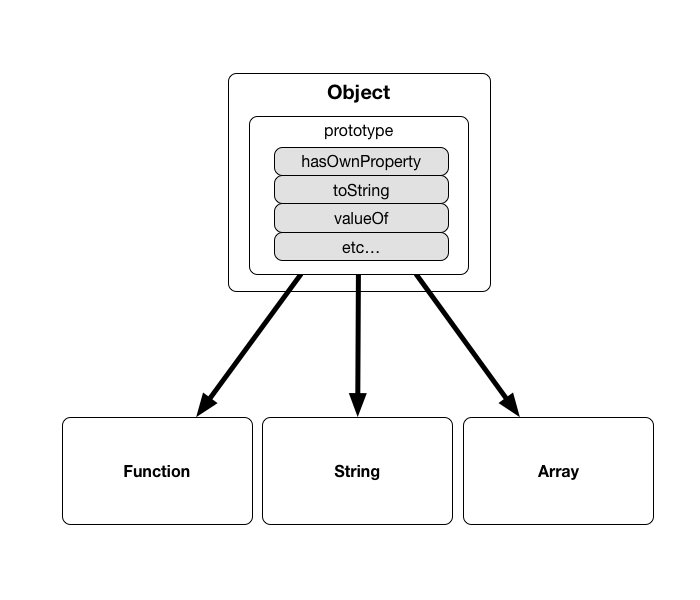
\includegraphics[width=80mm]{./fig/object-prototype.png}
\caption{すべてのオブジェクトは\texttt{Object}の\texttt{prototype}を継承している}
\end{figure}

具体的にどういうことかを見てみます。

先ほども登場した\texttt{toString}メソッドは、\texttt{Object}の\texttt{prototype}オブジェクトに定義があります。
次のように、\texttt{Object.prototype.toString}メソッドの実装自体も参照できます。

\begin{lstlisting}
// `Object.prototype`オブジェクトに`toString`メソッドの定義がある
console.log(typeof Object.prototype.toString); // => "function"
\end{lstlisting}

このような\texttt{prototype}オブジェクトに組み込まれているメソッドは\textbf{プロトタイプメソッド}と呼ばれます。
この書籍では\texttt{Object.prototype.toString}のようなプロトタイプメソッドを\texttt{Object\#toString}と短縮して表記します。

\begin{quote}
\texttt{Object.prototype.toString} =
\texttt{Object\#toString}
\end{quote}

\texttt{Object}のインスタンスは、この\texttt{Object.prototype}オブジェクトに定義されたメソッドやプロパティをインスタンス化したときに継承します。
つまり、オブジェクトリテラルや\texttt{new Object}でインスタンス化したオブジェクトは、\texttt{Object.prototype}に定義されたものが利用できるということです。

次のコードでは、オブジェクトリテラルで作成(インスタンス化)したオブジェクトから、\texttt{Object\#toString}メソッドを参照しています。
このときに、インスタンスの\texttt{toString}メソッドと\texttt{Object\#toString}は同じものとなることがわかります。

\begin{lstlisting}
const obj = {
    "key": "value"
};
// `obj`インスタンスは`Object.prototype`に定義されたものを継承する
// `obj.toString`は継承した`Object.prototype.toString`を参照している
console.log(obj.toString === Object.prototype.toString); // => true
// インスタンスからプロトタイプメソッドを呼び出せる
console.log(obj.toString()); // => "[object Object]"
\end{lstlisting}

このように\texttt{Object.prototype}に定義されている\texttt{toString}メソッドなどは、インスタンス作成時に自動的に継承されるため、\texttt{Object}のインスタンスから呼び出せます。
これによりオブジェクトリテラルで作成した空のオブジェクトでも、\texttt{Object\#toString}メソッドなどを呼び出せるようになっています。

このインスタンスから\texttt{prototype}オブジェクト上に定義されたメソッドを参照できる仕組みを\textbf{プロトタイプチェーン}と呼びます。
プロトタイプチェーンの仕組みについては「\href{../class/README.md}{クラス}」の章で扱うため、ここではインスタンスからプロトタイプメソッドを呼び出せるということがわかっていれば問題ありません。

\hypertarget{same-method-name-order}{%
\subsection{プロトタイプメソッドとインスタンスメソッドの優先順位}\label{same-method-name-order}}

プロトタイプメソッドと同じ名前のメソッドがインスタンスオブジェクトに定義されている場合もあります。
その場合には、インスタンスに定義したメソッドが優先して呼び出されます。

次のコードでは、\texttt{Object}のインスタンスである\texttt{customObject}に\texttt{toString}メソッドを定義しています。
実行してみると、プロトタイプメソッドよりも優先してインスタンスのメソッドが呼び出されていることがわかります。

\begin{lstlisting}
// オブジェクトのインスタンスにtoStringメソッドを定義
const customObject = {
    toString() {
        return "custom value";
    }
};
console.log(customObject.toString()); // => "custom value"
\end{lstlisting}

このように、インスタンスとプロトタイプオブジェクトで同じ名前のメソッドがある場合には、インスタンスのメソッドが優先されます。

\hypertarget{diff-in-operator-and-hasOwnProperty}{%
\subsection{\texorpdfstring{\texttt{in}演算子と\texttt{Object\#hasOwnProperty}メソッドの違い}{in演算子とObject\#hasOwnPropertyメソッドの違い}}\label{diff-in-operator-and-hasOwnProperty}}

「\href{../object/README.md}{オブジェクト}」の章で学んだ\texttt{Object\#hasOwnProperty}メソッドと\texttt{in}演算子の挙動の違いについて見ていきます。
2つの挙動の違いはこの章で紹介したプロトタイプオブジェクトに関係しています。

\texttt{hasOwnProperty}メソッドは、そのオブジェクト自身が指定したプロパティを持っているかを判定します。
一方、\texttt{in}演算子はオブジェクト自身が持っていなければ、そのオブジェクトの継承元である\texttt{prototype}オブジェクトまで探索して持っているかを判定します。
つまり、\texttt{in}演算子はインスタンスに実装されたメソッドなのか、プロトタイプオブジェクトに実装されたメソッドなのかを区別しません。

次のコードでは、空のオブジェクトが\texttt{toString}メソッドを持っているかを\texttt{Object\#hasOwnProperty}メソッドと\texttt{in}演算子でそれぞれ判定しています。
\texttt{hasOwnProperty}メソッドは\texttt{false}を返し、\texttt{in}演算子は\texttt{toString}メソッドがプロトタイプオブジェクトに存在するため\texttt{true}を返します。

\begin{lstlisting}
const obj = {};
// `obj`というオブジェクト自体に`toString`メソッドが定義されているわけではない
console.log(obj.hasOwnProperty("toString")); // => false
// `in`演算子は指定されたプロパティ名が見つかるまで親をたどるため、`Object.prototype`まで見にいく
console.log("toString" in obj); // => true
\end{lstlisting}

次のように、インスタンスが\texttt{toString}メソッドを持っている場合は、\texttt{hasOwnProperty}メソッドも\texttt{true}を返します。

\begin{lstlisting}
// オブジェクトのインスタンスにtoStringメソッドを定義
const obj = {
    toString() {
        return "custom value";
    }
};
// オブジェクトのインスタンスが`toString`メソッドを持っている
console.log(obj.hasOwnProperty("toString")); // => true
console.log("toString" in obj); // => true
\end{lstlisting}

\hypertarget{create-method}{%
\subsection{\texorpdfstring{オブジェクトの継承元を明示する\texttt{Object.create}メソッド}{オブジェクトの継承元を明示するObject.createメソッド}}\label{create-method}}

\texttt{Object.create}メソッドを使うと、第一引数に指定した\texttt{prototype}オブジェクトを継承した新しいオブジェクトを作成できます。

これまでの説明で、オブジェクトリテラルは\texttt{Object.prototype}オブジェクトを自動的に継承したオブジェクトを作成していることがわかりました。
オブジェクトリテラルで作成する新しいオブジェクトは、\texttt{Object.create}メソッドを使うことで次のように書けます。

\begin{lstlisting}
// const obj = {} と同じ意味
const obj = Object.create(Object.prototype);
// `obj`は`Object.prototype`を継承している
console.log(obj.hasOwnProperty === Object.prototype.hasOwnProperty); // => true
\end{lstlisting}

\hypertarget{inherit-object}{%
\subsection{ArrayもObjectを継承している}\label{inherit-object}}

\texttt{Object}と\texttt{Object.prototype}の関係と同じように、ビルトインオブジェクト\texttt{Array}も\texttt{Array.prototype}を持っています。
同じように、配列(\texttt{Array})のインスタンスは\texttt{Array.prototype}を継承します。
さらに、\texttt{Array.prototype}は\texttt{Object.prototype}を継承しているため、\texttt{Array}のインスタンスは\texttt{Object.prototype}も継承しています。

\begin{quote}
\texttt{Array}のインスタンス -\textgreater{}
\texttt{Array.prototype} -\textgreater{}
\texttt{Object.prototype}
\end{quote}

\texttt{Object.create}メソッドを使って\texttt{Array}と\texttt{Object}の関係をコードとして表現してみます。
この疑似コードは、\texttt{Array}コンストラクタの実装など、実際のものとは異なる部分があるため、あくまでイメージであることに注意してください。

\begin{lstlisting}
// このコードはイメージです!
// `Array`コンストラクタ自身は関数でもある
const Array = function() {};
// `Array.prototype`は`Object.prototype`を継承している
Array.prototype = Object.create(Object.prototype);
// `Array`のインスタンスは、`Array.prototype`を継承している
const array = Object.create(Array.prototype);
// `array`は`Object.prototype`を継承している
console.log(array.hasOwnProperty === Object.prototype.hasOwnProperty); // => true
\end{lstlisting}

このように、\texttt{Array}のインスタンスも\texttt{Object.prototype}を継承しているため、
\texttt{Object.prototype}に定義されているメソッドを利用できます。

次のコードでは、\texttt{Array}のインスタンスから\texttt{Object\#hasOwnProperty}メソッドが参照できていることがわかります。

\begin{lstlisting}
const array = [];
// `Array`のインスタンス -> `Array.prototype` -> `Object.prototype`
console.log(array.hasOwnProperty === Object.prototype.hasOwnProperty); // => true
\end{lstlisting}

このような\texttt{hasOwnProperty}メソッドの参照が可能なのもプロトタイプチェーンという仕組みによるものです。

ここでは、\texttt{Object.prototype}はすべてのオブジェクトの親となるオブジェクトであることを覚えておくだけで問題ありません。
これにより、\texttt{Array}や\texttt{String}などのインスタンスも\texttt{Object.prototype}が持つメソッドを利用できる点を覚えておきましょう。

また、\texttt{Array.prototype}などもそれぞれ独自のメソッドを定義しています。
たとえば、\texttt{Array\#toString}メソッドもそのひとつです。
そのため、配列のインスタンスで\texttt{toString}メソッドを呼び出すと\texttt{Array\#toString}が優先して呼び出されます。

\begin{lstlisting}
const numbers = [1, 2, 3];
// `Array#toString`が定義されているため、`Object#toString`とは異なる形式となる
console.log(numbers.toString()); // => "1,2,3"
\end{lstlisting}

\begin{tcolorbox}[title=\texttt{Object.prototype}を継承しないオブジェクト]\label{not-inherit-object}

\texttt{Object}はすべてのオブジェクトの親になるオブジェクトであると言いましたが、例外もあります。

イディオム(慣習的な書き方)ですが、\texttt{Object.create(null)}とすることで\texttt{Object.prototype}を継承しないオブジェクトを作成できます。
これにより、プロパティやメソッドをまったく持たない本当に\textbf{空のオブジェクト}を作れます。

\begin{lstlisting}
// 親がnull、つまり親がいないオブジェクトを作る
const obj = Object.create(null);
// Object.prototypeを継承しないため、hasOwnPropertyが存在しない
console.log(obj.hasOwnProperty); // => undefined
\end{lstlisting}

\texttt{Object.create}メソッドはES5から導入されました。
\texttt{Object.create}メソッドは\texttt{Object.create(null)}というイディオムで、一部ライブラリなどで\texttt{Map}オブジェクトの代わりとして利用されていました。
Mapとはキーと値の組み合わせを保持するためのオブジェクトです。

ただのオブジェクトもMapとよく似た性質を持っていますが、最初からいくつかのプロパティが存在しアクセスできてしまいます。
なぜなら、\texttt{Object}のインスタンスはデフォルトで\texttt{Object.prototype}を継承するため、\texttt{toString}などのプロパティ名がオブジェクトを作成した時点で存在するためです。そのため、\texttt{Object.create(null)}で\texttt{Object.prototype}を継承しないオブジェクトを作成し、そのオブジェクトが\texttt{Map}の代わりとして使われていました。

\begin{lstlisting}
// 空オブジェクトを作成
const obj = {};
// "toString"という値を定義してないのに、"toString"が存在している
console.log(obj["toString"]);// Function 
// Mapのような空オブジェクト
const mapLike = Object.create(null);
// toStringキーは存在しない
console.log(mapLike["toString"]); // => undefined
\end{lstlisting}

しかし、ES2015からは、本物の\texttt{Map}が利用できるため、\texttt{Object.create(null)}を\texttt{Map}の代わりに利用する必要はありません。
\texttt{Map}については「\href{../map-and-set/README.md}{Map/Set}」の章で詳しく紹介します。

\begin{lstlisting}
const map = new Map();
// toStringキーは存在しない
console.log(map.has("toString")); // => false
\end{lstlisting}
\end{tcolorbox}

\hypertarget{conclusion}{%
\section{まとめ}\label{conclusion}}

この章では、プロトタイプオブジェクトについて学びました。

\begin{itemize}
\item
  プロトタイプオブジェクトはオブジェクトの作成時に自動的に作成される
\item
  \texttt{Object}のプロトタイプオブジェクトには\texttt{toString}などのプロトタイプメソッドが定義されている
\item
  ほとんどのオブジェクトは\texttt{Object.prototype}を継承することで\texttt{toString}メソッドなどを呼び出せる
\item
  プロトタイプメソッドとインスタンスメソッドではインスタンスメソッドが優先される
\item
  \texttt{Object.create}メソッドを使うことでプロトタイプオブジェクトを継承しないオブジェクトを作成できる
\end{itemize}

プロトタイプオブジェクトに定義されているメソッドがどのように参照されているかを確認しました。
このプロトタイプの詳しい仕組みについては「\href{../class/README.md}{クラス}」の章で改めて解説します。

\hypertarget{array}{%
\chapter{配列}\label{array}}\index{はいれつ@配列}
\thispagestyle{frontheadings}

配列はJavaScriptの中でもよく使われるオブジェクトです。

配列とは値に順序をつけて格納できるオブジェクトです。
配列に格納したそれぞれの値のことを\textbf{\textgt{要素}}\index{ようそ@要素}\index{はいれつ@配列!ようそ@要素}、それぞれの要素の位置のことを\textbf{\textgt{インデックス}}\index{いんでっくす@インデックス}\index{はいれつ@配列!いんでっくす@インデックス}(\texttt{index}\index{index})と呼びます。
インデックスは先頭の要素から\texttt{0}、\texttt{1}、\texttt{2}のように\texttt{0}からはじまる連番となります。

またJavaScriptにおける配列は可変長です。
そのため配列を作成後に配列へ要素を追加したり、配列から要素を削除できます。

この章では、配列の基本的な操作と配列を扱う場合においてのパターンについて学びます。

\hypertarget{create-and-access}{%
\section{配列の作成とアクセス}\label{create-and-access}}

配列の作成と要素へのアクセス方法は「\hyperlink{data-type-and-literal}{データ型とリテラル}」の章の「\hyperlink{array-literal}{配列リテラル}」ですでに紹介していますが、
もう一度振り返ってみましょう。

配列の作成には配列リテラルを使います。
配列リテラル\index{はいれつりてらる@配列リテラル}(\texttt{[}と\texttt{]}\index{[]@\texttt{[]}})の中に要素をカンマ(\texttt{,})区切りで記述するだけです。

\begin{lstlisting}
const emptyArray = [];
const numbers = [1, 2, 3];
// 2次元配列(配列の配列)
const matrix = [
    ["a", "b"],
    ["c", "d"]
];
\end{lstlisting}

作成した配列の要素へのインデックスとなる数値を、\texttt{配列[インデックス]}と記述することで、
そのインデックスの要素を配列から読み取れます。
配列の先頭要素のインデックスは\texttt{0}となります。配列のインデックスは、\texttt{0}以上\texttt{$2^{32} - 1$}未満の整数となります。

\begin{lstlisting}
const array = ["one", "two", "three"];
console.log(array[0]); // => "one"
\end{lstlisting}

2次元配列(配列の配列)からの値の読み取りも同様に\texttt{配列[インデックス]}でアクセスできます。
\texttt{配列[0][0]}は、配列の\texttt{0}番目の要素である配列(\texttt{["a", "b"]})の\texttt{0}番目の要素を読み取ります。

\begin{lstlisting}
// 2次元配列(配列の配列)
const matrix = [
    ["a", "b"],
    ["c", "d"]
];
console.log(matrix[0][0]); // => "a"
\end{lstlisting}

配列の\texttt{length}\index{はいれつ@配列!length@\texttt{length}}\index{length@\texttt{length}}プロパティは配列の要素の数を返します。
そのため、配列の最後の要素へアクセスするには
\texttt{array.length - 1}
をインデックスとして利用できます。

\begin{lstlisting}
const array = ["one", "two", "three"];
console.log(array.length); // => 3
// 配列の要素数 - 1 が 最後の要素のインデックスとなる
console.log(array[array.length - 1]); // => "three"
\end{lstlisting}

一方、存在しないインデックスにアクセスした場合はどうなるでしょうか? JavaScriptでは、存在しないインデックスに対してアクセスした場合に、例外ではなく\texttt{undefined}\index{undefined@\texttt{undefined}}を返します。

\begin{lstlisting}
const array = ["one", "two", "three"];
// arrayにはインデックスが100の要素は定義されていない
console.log(array[100]); // => undefined
\end{lstlisting}

これは、配列がオブジェクトであることを考えると、次のように存在しないプロパティへアクセスしているのと原理は同じです。
オブジェクトでも、存在しないプロパティへアクセスした場合には\texttt{undefined}が返ってきます。

\begin{lstlisting}
const obj = {
    "0": "one",
    "1": "two",
    "2": "three",
    "length": 3
};
// obj["100"]は定義されていないためundefinedが返る
console.log(obj[100]); // => undefined
\end{lstlisting}

また、配列は常に\texttt{length}の数だけ要素を持っているとは限りません。
次のように、配列リテラルでは値を省略することで、未定義の要素を含めることができます。
このような、配列の中に隙間があるものを\textbf{\textgt{疎な配列}}\index{そなはいれつ@疎な配列}\index{はいれつ@配列!そ@疎}と呼びます。
一方、隙間がなくすべてのインデックスに要素がある配列を\textbf{\textgt{密な配列}}\index{みつなはいれつ@密な配列}\index{はいれつ@配列!みつ@密}と呼びます。

\begin{lstlisting}
// 未定義の箇所が1つ含まれる疎な配列
// インデックスが1の値を省略しているので、カンマが2つ続いていることに注意
const sparseArray = [1,, 3];
console.log(sparseArray.length); // => 3 
// 1番目の要素は存在しないため undefined が返る
console.log(sparseArray[1]); // => undefined
\end{lstlisting}

\hypertarget{detect-array}{%
\section{オブジェクトが配列かどうかを判定する}\label{detect-array}}

あるオブジェクトが配列かどうかを判定するには\texttt{Array.isArray}\index{Array.isArray@\texttt{Array.isArray}}メソッドを利用します。
\texttt{Array.isArray}メソッドは引数が配列ならば\texttt{true}を返します。

\begin{lstlisting}
const obj = {};
const array = [];
console.log(Array.isArray(obj)); // => false
console.log(Array.isArray(array)); // => true
\end{lstlisting}

また、\texttt{typeof}演算子では配列かどうかを判定することはできません。
配列もオブジェクトの一種であるため、\texttt{typeof}演算子の結果が\texttt{"object"}となるためです。

\begin{lstlisting}
const array = [];
console.log(typeof array); // => "object"
\end{lstlisting}

\begin{tcolorbox}[title=TypedArray\,\protect\icon{fig/es2015.eps}]\label{typed-array}\index{TypedArray@\texttt{TypedArray}}

JavaScriptの配列は可変長のみですが、\texttt{TypedArray}という固定長でかつ型つきの配列を扱う別のオブジェクトが存在します。
\texttt{TypedArray}はバイナリデータのバッファを示すために使われるデータ型で、WebGLやバイナリを扱う場面で利用されます。
文字列や数値などのプリミティブ型の値はそのままでは扱えないため、通常の配列とは用途や使い勝手が異なります。

また、TypedArrayは\texttt{Array.isArray}のメソッドの結果が\texttt{false}となることからも別物と考えてよいでしょう。

\begin{lstlisting}
// TypedArrayを作成
const typedArray = new Int8Array(8);
console.log(Array.isArray(typedArray)); // => false
\end{lstlisting}

そのため、JavaScriptで配列といった場合には\texttt{Array}を示します。
\end{tcolorbox}

\hypertarget{array-destructuring}{%
\section[配列と分割代入]{配列と分割代入\,\protect\icon{fig/es2015.eps}}\label{array-destructuring}}\index{ぶんかつだいにゅう@分割代入}\index{はいれつ@配列!ぶんかつだいにゅう@分割代入}

配列の指定したインデックスの値を変数として定義し直す場合には、分割代入(Destructuring
assignment\index{Destructuring assignment})が利用できます。

配列の分割代入では、左辺に配列リテラルのような構文で定義したい変数名を書きます。
右辺の配列から対応するインデックスの要素が、左辺で定義した変数に代入されます。

次のコードでは、左辺に定義した変数に対して、右辺の配列から対応するインデックスの要素が代入されます。
\texttt{first}にはインデックスが\texttt{0}の要素、\texttt{second}にはインデックスが\texttt{1}の要素、\texttt{third}にはインデックスが\texttt{2}の要素が代入されます。

\begin{lstlisting}
const array = ["one", "two", "three"];
const [first, second, third] = array;
console.log(first);  // => "one"
console.log(second); // => "two"
console.log(third);  // => "three"
\end{lstlisting}

\begin{tcolorbox}[enhanced jigsaw,breakable,title=undefinedの要素と未定義の要素の違い]\label{diff-undefined-and-no-element}\index{undefined@\texttt{undefined}}

疎な配列で該当するインデックスに要素がない場合は\texttt{undefined}を返します。
しかし、\texttt{undefined}という値も存在するため、配列に\texttt{undefined}という値がある場合に区別できません。

次のコードでは、\texttt{undefined}という値を要素として定義した密な配列と、要素そのものがない疎な配列を定義しています。
どちらも要素にアクセスした結果は\texttt{undefined}となり、区別できていないことがわかります。

\begin{lstlisting}
// 要素としてundefinedを持つ密な配列
const denseArray = [1, undefined, 3];
// 要素そのものがない疎な配列
const sparseArray = [1, , 3];
console.log(denseArray[1]); // => undefined
console.log(sparseArray[1]); // => undefined
\end{lstlisting}

この違いを見つける方法として利用できるのが\texttt{Object\#hasOwnProperty}\index{Object\#hasOwnProperty@\texttt{Object\#hasOwnProperty}}メソッドです。
\texttt{hasOwnProperty}\index{hasOwnProperty@\texttt{hasOwnProperty}}メソッドを使うことで、配列の指定したインデックスに要素自体が存在するかを判定できます。

\begin{lstlisting}
const denseArray = [1, undefined, 3];
const sparseArray = [1, , 3];
// 要素自体はundefined値が存在する
console.log(denseArray.hasOwnProperty(1)); // => true
// 要素自体がない
console.log(sparseArray.hasOwnProperty(1)); // => false
\end{lstlisting}
\end{tcolorbox}

\hypertarget{search-element}{%
\section{配列から要素を検索}\label{search-element}}\index{はいれつ@配列!けんさく@検索}

配列から指定した要素を検索する目的には、 主に次の3つがあります。

\begin{itemize}
\item
  その要素のインデックスが欲しい場合
\item
  その要素自体が欲しい場合
\item
  その要素が含まれているかという真偽値が欲しい場合
\end{itemize}

配列にはそれぞれに対応したメソッドが用意されているため、目的別に見ていきます。

\hypertarget{indexof}{%
\subsection{インデックスを取得}\label{indexof}}\index{いんでっくす@インデックス!しゅとく@取得}

指定した要素が配列のどの位置にあるかを知りたい場合、\texttt{Array\#indexOf}\index{Array\#indexOf@\texttt{Array\#indexOf}}メソッドや\texttt{Array\#findIndex}\index{Array\#findIndex@\texttt{Array\#findIndex}}メソッド\,\protect\iconl{fig/es2015.eps}\,を利用します。
要素の位置のことを\textbf{インデックス}(\texttt{index})と呼ぶため、メソッド名にも\texttt{index}という名前が入っています。

次のコードでは、\texttt{Array\#indexOf}メソッドを利用して、配列の中から\texttt{"JavaScript"}という文字列のインデックスを取得しています。
\texttt{indexOf}メソッドは引数と厳密等価演算子(\texttt{===})で一致する要素があるなら、その要素のインデックスを返し、該当する要素がない場合は\texttt{-1}を返します。
\texttt{indexOf}\index{indexOf@\texttt{indexOf}}メソッドは先頭から検索して見つかった要素のインデックスを返します。
\texttt{indexOf}メソッドには対となる\texttt{Array\#lastIndexOf}\index{Array\#lastIndexOf@\texttt{Array\#lastIndexOf}}メソッドがあり、\texttt{lastIndexOf}\index{lastIndexOf@\texttt{lastIndexOf}}メソッドでは末尾から検索した結果が得られます。

\begin{lstlisting}
const array = ["Java", "JavaScript", "Ruby"];
const indexOfJS = array.indexOf("JavaScript");
console.log(indexOfJS); // => 1
console.log(array[indexOfJS]); // => "JavaScript"
// "JS" という要素はないため -1 が返される
console.log(array.indexOf("JS")); // => -1
\end{lstlisting}

\texttt{indexOf}メソッドは配列からプリミティブな要素を発見できますが、オブジェクトは持っているプロパティが同じでも別オブジェクトだと異なるものとして扱われます。
次のコードを見ると、同じプロパティを持つ異なるオブジェクトは、\texttt{indexOf}メソッドでは見つけることができません。
これは、異なる参照を持つオブジェクト同士は\texttt{===}で比較しても一致しないためです。

\begin{lstlisting}
const obj = { key: "value" };
const array = ["A", "B", obj];
console.log(array.indexOf({ key: "value" })); // => -1
// リテラルは新しいオブジェクトを作るため、異なるオブジェクトだと判定される
console.log(obj === { key: "value" }); // => false
// 等価のオブジェクトを検索してインデックスを返す
console.log(array.indexOf(obj)); // => 2
\end{lstlisting}

このように、異なるオブジェクトだが値は同じものを見つけたい場合には、\texttt{Array\#findIndex}\index{Array\#findIndex@\texttt{Array\#findIndex}}メソッドが利用できます。
\texttt{findIndex}\index{findIndex@\texttt{findIndex}}メソッドの引数には配列の各要素をテストする関数をコールバック関数として渡します。
\texttt{indexOf}メソッドとは異なり、テストする処理を自由に書けます。
これにより、プロパティの値が同じ要素を配列から見つけて、その要素のインデックスが得られます。

\begin{lstlisting}
// colorプロパティを持つオブジェクトの配列
const colors = [
    { "color": "red" },
    { "color": "green" },
    { "color": "blue" }
];
// colorプロパティが"blue"のオブジェクトのインデックスを取得
const indexOfBlue = colors.findIndex((obj) => {
    return obj.color === "blue";
});
console.log(indexOfBlue); // => 2
console.log(colors[indexOfBlue]); // => { "color": "blue" }
\end{lstlisting}

\hypertarget{find}{%
\subsection{条件に一致する要素を取得}\label{find}}

配列から要素を取得する方法としてインデックスを使うこともできます。
先ほどのように\texttt{findIndex}メソッドでインデックスを取得し、そのインデックスで配列へアクセスすればよいだけです。

しかし、\texttt{findIndex}メソッドを使って要素を取得するケースでは、
そのインデックスが欲しいのか、またはその要素自体が欲しいのかがコードとして明確ではありません。

より明確に要素自体が欲しいということを表現するには、\texttt{Array\#find}\index{Array\#find@\texttt{Array\#find}}メソッド\,\protect\iconl{fig/es2015.eps}\,が使えます。
\texttt{find}\index{find@\texttt{find}}メソッドには、\texttt{findIndex}メソッドと同様にテストする関数をコールバック関数として渡します。
\texttt{find}メソッドの返り値は、要素そのものとなり、要素が存在しない場合は\texttt{undefined}を返します。

\begin{lstlisting}
// colorプロパティを持つオブジェクトの配列
const colors = [
    { "color": "red" },
    { "color": "green" },
    { "color": "blue" }
];
// colorプロパティが"blue"のオブジェクトを取得
const blueColor = colors.find((obj) => {
    return obj.color === "blue";
});
console.log(blueColor); // => { "color": "blue" }
// 該当する要素がない場合はundefinedを返す
const whiteColor = colors.find((obj) => {
    return obj.color === "white";
});
console.log(whiteColor); // => undefined
\end{lstlisting}

\hypertarget{slice}{%
\subsection{指定範囲の要素を取得}\label{slice}}

配列から指定範囲の要素を取り出す方法として\texttt{Array\#slice}\index{Array\#slice@\texttt{Array\#slice}}メソッドが利用できます。
\texttt{slice}\index{slice@\texttt{slice}}メソッドは第一引数に開始位置、第二引数に終了位置を指定することで、その範囲を取り出した新しい配列を返します。
第二引数は省略でき、省略した場合は配列の末尾が終了位置となります。

\begin{lstlisting}
const array = ["A", "B", "C", "D", "E"];
// インデックス1から4の範囲を取り出す
console.log(array.slice(1, 4)); // => ["B", "C", "D"]
// 第二引数を省略した場合は、第一引数から末尾の要素までを取り出す
console.log(array.slice(1)); // => ["B", "C", "D", "E"]
// マイナスを指定すると後ろから数えた位置となる
console.log(array.slice(-1)); // => ["E"]
// 第一引数 > 第二引数の場合、常に空配列を返す
console.log(array.slice(4, 1)); // => []
\end{lstlisting}

\hypertarget{get-boolean}{%
\subsection{真偽値を取得}\label{get-boolean}}\index{しんぎち@真偽値}

最後に、指定した要素が配列に含まれているかを知る方法について見ていきます。
インデックスや要素が取得できれば、その要素は配列に含まれているということはわかります。

しかし、指定した要素が含まれているか\textbf{だけ}を知りたい場合に、
\texttt{Array\#findIndex}メソッドや\texttt{Array\#find}メソッドは過剰な機能を持っています。
そのコードを読んだ人には、取得したインデックスや要素を何に使うのかが明確ではありません。

次のコードは、\texttt{Array\#indexOf}メソッドを利用し、該当する要素が含まれているかを判定しています。
\texttt{indexOf}メソッドの結果を\texttt{indexOfJS}に代入していますが、含まれているかを判定する以外には利用していません。
コードを隅々まで読まないといけないため、意図が明確ではなくコードの読みづらさにつながります。

\begin{lstlisting}
const array = ["Java", "JavaScript", "Ruby"];
// indexOfメソッドは含まれていないときのみ-1を返すことを利用
const indexOfJS = array.indexOf("JavaScript");
if (indexOfJS !== -1) {
    console.log("配列にJavaScriptが含まれている");
    // ... いろいろな処理 ...
    // indexOfJSは、含まれているのかの判定以外には利用していない
}
\end{lstlisting}

そこで、ES2016で導入された\texttt{Array\#includes}\index{Array\#includes@\texttt{Array\#includes}}メソッド\,\protect\iconl{fig/es2016.eps}\,を利用します。
\texttt{Array\#includes}メソッドは配列に指定要素が含まれているかを判定します。
\texttt{includes}\index{includes@\texttt{includes}}メソッドは真偽値を返すので、\texttt{indexOf}メソッドを使った場合に比べて意図が明確になります。
前述のコードでは次のように\texttt{includes}メソッドを使うべきでしょう。

\begin{lstlisting}
const array = ["Java", "JavaScript", "Ruby"];
// includesは含まれているならtrueを返す
if (array.includes("JavaScript")) {
    console.log("配列にJavaScriptが含まれている");
}
\end{lstlisting}

\texttt{includes}メソッドは、\texttt{indexOf}メソッドと同様、異なるオブジェクトだが値が同じものを見つけたい場合には利用できません。
\texttt{Array\#find}メソッドのようにテストするコールバック関数を利用して、真偽値を得るには\texttt{Array\#some}\index{Array\#some@\texttt{Array\#some}}メソッドを利用できます。

\texttt{Array\#some}メソッドはテストするコールバック関数にマッチする要素があるなら\texttt{true}を返し、存在しない場合は\texttt{false}を返します
(「\hyperlink{loop-and-iteration}{ループと反復処理}」の章の「\hyperlink{array-some}{配列の\texttt{some}メソッド}」を参照)。

\begin{lstlisting}
// colorプロパティを持つオブジェクトの配列
const colors = [
    { "color": "red" },
    { "color": "green" },
    { "color": "blue" }
];
// colorプロパティが"blue"のオブジェクトがあるかどうか
const isIncludedBlueColor = colors.some((obj) => {
    return obj.color === "blue";
});
console.log(isIncludedBlueColor); // => true
\end{lstlisting}

\hypertarget{add-and-delete}{%
\section{追加と削除}\label{add-and-delete}}

配列は可変長であるため、作成後の配列に対して要素を追加、削除できます。

要素を配列の末尾へ追加するには\texttt{Array\#push}\index{Array\#push@\texttt{Array\#push}}が利用できます。
一方、末尾から要素を削除するには\texttt{Array\#pop}\index{Array\#pop@\texttt{Array\#pop}}が利用できます。

\begin{lstlisting}
const array = ["A", "B", "C"];
array.push("D"); // "D"を末尾に追加
console.log(array); // => ["A", "B", "C", "D"]
const poppedItem = array.pop(); // 最末尾の要素を削除し、その要素を返す 
console.log(poppedItem); // => "D"
console.log(array); // => ["A", "B", "C"]
\end{lstlisting}

要素を配列の先頭へ追加するには\texttt{Array\#unshift}\index{Array\#unshift@\texttt{Array\#unshift}}が利用できます。
一方、配列の先頭から要素を削除するには\texttt{Array\#shift}\index{Array\#shift@\texttt{Array\#shift}}が利用できます。

\begin{lstlisting}
const array = ["A", "B", "C"];
array.unshift("S"); // "S"を先頭に追加
console.log(array); // => ["S", "A", "B", "C"]
const shiftedItem = array.shift(); // 先頭の要素を削除 
console.log(shiftedItem); // => "S"
console.log(array); // => ["A", "B", "C"]
\end{lstlisting}

\hypertarget{concat}{%
\section{配列同士を結合}\label{concat}}\index{はいれつ@配列!けつごう@結合}

\texttt{Array\#concat}\index{Array\#concat@\texttt{Array\#concat}}メソッドを使うことで配列と配列を結合した新しい配列を作成できます。

\begin{lstlisting}
const array = ["A", "B", "C"];
const newArray = array.concat(["D", "E"]);
console.log(newArray); // => ["A", "B", "C", "D", "E"]
\end{lstlisting}

また、\texttt{concat}\index{concat@\texttt{concat}}メソッドは配列だけではなく任意の値を要素として結合できます。

\begin{lstlisting}
const array = ["A", "B", "C"];
const newArray = array.concat("新しい要素");
console.log(newArray); // => ["A", "B", "C", "新しい要素"]
\end{lstlisting}

\hypertarget{spread}{%
\section[配列の展開]{配列の展開\,\protect\icon{fig/es2015.eps}}\label{spread}}\index{はいれつ@配列!てんかい@展開}

\texttt{...}(Spread構文)を使うことで、配列リテラル中に既存の配列を展開できます。

次のコードでは、配列リテラルの末尾に配列を展開しています。
これは、\texttt{Array\#concat}メソッドで配列同士を結合するのと同じ結果になります。

\begin{lstlisting}
const array = ["A", "B", "C"];
// Spread構文を使った場合
const newArray = ["X", "Y", "Z", ...array];
// concatメソッドの場合
const newArrayConcat = ["X", "Y", "Z"].concat(array);
console.log(newArray); // => ["X", "Y", "Z", "A", "B", "C"]
console.log(newArrayConcat); // => ["X", "Y", "Z", "A", "B", "C"]
\end{lstlisting}

Spread構文は、\texttt{concat}メソッドとは異なり、配列リテラル中の任意の位置に配列を展開できます。
そのため、次のように要素の途中に配列を展開することも可能です。

\begin{lstlisting}
const array = ["A", "B", "C"];
const newArray = ["X", ...array, "Z"];
console.log(newArray); // => ["X", "A", "B", "C", "Z"]
\end{lstlisting}

\hypertarget{flat}{%
\section[配列をフラット化]{配列をフラット化\,\protect\icon{fig/es2019.eps}}\label{flat}}\index{はいれつ@配列!ふらっとか@フラット化}\index{ふらっとか@フラット化}

\texttt{Array\#flat}\index{Array\#flat@\texttt{Array\#flat}}メソッド\,\protect\iconl{fig/es2019.eps}\,を使うことで、多次元配列をフラットな配列に変換できます。
引数を指定しなかった場合は1段階のみのフラット化ですが、引数に渡す数値でフラット化する深さを指定できます。
配列をすべてフラット化する場合には、無限を意味する\texttt{Infinity}\index{Infinity@\texttt{Infinity}}を値として渡すことで実現できます。

\begin{lstlisting}
const array = [[["A"], "B"], "C"];
// 引数なしは 1 を指定した場合と同じ
console.log(array.flat()); // => [["A"], "B", "C"]
console.log(array.flat(1)); // => [["A"], "B", "C"]
console.log(array.flat(2)); // => ["A", "B", "C"]
// すべてをフラット化するには Inifinity を渡す
console.log(array.flat(Infinity)); // => ["A", "B", "C"]
\end{lstlisting}

また、\texttt{Array\#flat}メソッドは必ず新しい配列を作成して返すメソッドです。
そのため、これ以上フラット化できない配列をフラット化しても、同じ要素を持つ新しい配列を返します。

\begin{lstlisting}
const array = ["A", "B", "C"];
console.log(array.flat()); // => ["A", "B", "C"]
\end{lstlisting}

\hypertarget{delete-element}{%
\section{配列から要素を削除}\label{delete-element}}\index{はいれつ@配列!さくじょ@削除}

\hypertarget{splice}{%
\subsection{\texorpdfstring{\texttt{Array\#splice}}{Array\#splice}}\label{splice}}\index{Array\#splice@\texttt{Array\#splice}}

配列の先頭や末尾の要素を削除する場合は\texttt{Array\#shift}や\texttt{Array\#pop}で行えます。
しかし、配列の任意のインデックスの要素を削除できません。
配列の任意のインデックスの要素を削除するには\texttt{Array\#splice}を利用できます。

\texttt{Array\#splice}メソッドを利用すると、削除した要素を自動で詰めることができます。
\texttt{Array\#splice}メソッドは指定したインデックスから、指定した数だけ要素を取り除き、必要ならば要素を同時に追加できます。

\begin{lstlisting}
const array = [];
array.splice(インデックス, 削除する要素数);
// 削除と同時に要素の追加もできる
array.splice(インデックス, 削除する要素数, ...追加する要素);
\end{lstlisting}

たとえば、配列のインデックスが\texttt{1}の要素を削除するには、インデックス\texttt{1}から\texttt{1}つの要素を削除するという指定をする必要があります。
このとき、削除した要素は自動で詰められるため、疎な配列にはなりません。

\begin{lstlisting}
const array = ["a", "b", "c"];
// 1番目から1つの要素("b")を削除
array.splice(1, 1);
console.log(array); // => ["a", "c"]
console.log(array.length); // => 2
console.log(array[1]); // => "c"
// すべて削除
array.splice(0, array.length);
console.log(array.length); // => 0
\end{lstlisting}

\hypertarget{assign-to-length}{%
\subsection{\texorpdfstring{\texttt{length}プロパティへの代入}{lengthプロパティへの代入}}\label{assign-to-length}}\index{length@\texttt{length}}\index{はいれつ@配列!length@\texttt{length}}

配列のすべての要素を削除することは\texttt{Array\#splice}で行えますが、
配列の\texttt{length}プロパティへの代入を利用した方法もあります。

\begin{lstlisting}
const array = [1, 2, 3];
array.length = 0; // 配列を空にする
console.log(array); // => []
\end{lstlisting}

配列の\texttt{length}プロパティへ\texttt{要素数}を代入すると、その要素数に配列が切り詰められます。
つまり、\texttt{length}プロパティへ\texttt{0}を代入すると、インデックスが\texttt{0}以降の要素がすべて削除されます。

\hypertarget{assign-empty-array}{%
\subsection{空の配列を代入}\label{assign-empty-array}}

最後に、その配列の要素を削除するのではなく、新しい空の配列を変数へ代入する方法です。
次のコードでは、\texttt{array}変数に空の配列を代入することで、\texttt{array}に空の配列を参照させています。

\begin{lstlisting}
let array = [1, 2, 3];
console.log(array.length); // => 3
// 新しい配列で変数を上書き
array = [];
console.log(array.length); // => 0
\end{lstlisting}

元々、\texttt{array}変数が参照していた\texttt{[1, 2, 3]}はどこからも参照されなくなり、ガベージコレクションによりメモリから解放されます。

また、\texttt{const}で宣言した配列の場合は変数に対して再代入できないため、この手法は使えません。
そのため、再代入をしたい場合は\texttt{let}または\texttt{var}で変数宣言をする必要があります。

\begin{lstlisting}
const array = [1, 2, 3];
console.log(array.length); // => 3
// constで宣言された変数には再代入できない
array = []; // TypeError: invalid assignment to const `array' が発生
\end{lstlisting}

\hypertarget{mutable-immutable}{%
\section{破壊的なメソッドと非破壊的なメソッド}\label{mutable-immutable}}\index{はかいてきなめそっど@破壊的なメソッド}\index{ひはかいてきなめそっど@非破壊的なメソッド}

これまで紹介してきた配列を変更するメソッドには、破壊的なメソッドと非破壊的メソッドがあります。この破壊的なメソッドと非破壊的メソッドの違いを知ることは、意図しない結果を避けるために重要です。
破壊的なメソッドとは、配列オブジェクトそのものを変更し、変更した配列または変更箇所を返すメソッドです。
非破壊的メソッドとは、配列オブジェクトのコピーを作成してから変更し、そのコピーした配列を返すメソッドです。

破壊的なメソッドの例として、配列に要素を追加する\texttt{Array\#push}\index{Array\#push@\texttt{Array\#push}}メソッドがあります。
\texttt{push}\index{push@\texttt{push}}メソッドは、\texttt{myArray}の配列そのものへ要素を追加しています。
その結果\texttt{myArray}変数の参照する配列が変更されるため破壊的なメソッドです。

\begin{lstlisting}
const myArray = ["A", "B", "C"];
const result = myArray.push("D"); 
// pushの返り値は配列ではなく、追加後の配列のlength
console.log(result); // => 4
// myArrayが参照する配列そのものが変更されている
console.log(myArray); // => ["A", "B", "C", "D"]
\end{lstlisting}

非破壊的なメソッドの例として、配列に要素を結合する\texttt{Array\#concat}\index{Array\#concat@\texttt{Array\#concat}}メソッドがあります。
\texttt{concat}\index{concat@\texttt{concat}}メソッドは、\texttt{myArray}をコピーした配列に対して要素を結合し、その配列を返します。
\texttt{myArray}変数の参照する配列は変更されないため非破壊的なメソッドです。

\begin{lstlisting}
const myArray = ["A", "B", "C"];
// concatの返り値は結合済みの新しい配列
const newArray = myArray.concat("D");
console.log(newArray); // => ["A", "B", "C", "D"]
// myArrayは変更されていない
console.log(myArray); // => ["A", "B", "C"]
// newArrayとmyArrayは異なる配列オブジェクト
console.log(myArray === newArray); // => false
\end{lstlisting}

JavaScriptにおいて破壊的なメソッドと非破壊的メソッドを名前から見分ける方法はありません。
また、配列を返す破壊的なメソッドもあるため、返り値からも判別できません。
たとえば、\texttt{Array\#sort}\index{Array\#sort@\texttt{Array\#sort}}メソッドは返り値がソート済みの配列ですが破壊的メソッドです。

次の表で紹介するメソッド\footnote{\url{https://developer.mozilla.org/ja/docs/Web/JavaScript/Reference/Global_Objects/Array/}}は破壊的なメソッドです。

\begin{small}
\begin{longtable}[l]{p{73mm}|p{67mm}}
\hline\rowcolor[gray]{0.85}\rule[0mm]{0mm}{4mm}{\textgt メソッド名} & {\textgt 返り値}\tabularnewline
\hline
\endhead
\href{https://developer.mozilla.org/ja/docs/Web/JavaScript/Reference/Global_Objects/Array/pop}{\texttt{Array.prototype.pop}}
& 配列の末尾の値\tabularnewline
\href{https://developer.mozilla.org/ja/docs/Web/JavaScript/Reference/Global_Objects/Array/push}{\texttt{Array.prototype.push}}
& 変更後の配列のlength\tabularnewline
\href{https://developer.mozilla.org/ja/docs/Web/JavaScript/Reference/Global_Objects/Array/splice}{\texttt{Array.prototype.splice}}
& 取り除かれた要素を含む配列\tabularnewline
\href{https://developer.mozilla.org/ja/docs/Web/JavaScript/Reference/Global_Objects/Array/reverse}{\texttt{Array.prototype.reverse}}
& 反転した配列\tabularnewline
\href{https://developer.mozilla.org/ja/docs/Web/JavaScript/Reference/Global_Objects/Array/shift}{\texttt{Array.prototype.shift}}
& 配列の先頭の値\tabularnewline
\href{https://developer.mozilla.org/ja/docs/Web/JavaScript/Reference/Global_Objects/Array/sort}{\texttt{Array.prototype.sort}}
& ソートした配列\tabularnewline
\href{https://developer.mozilla.org/ja/docs/Web/JavaScript/Reference/Global_Objects/Array/unshift}{\texttt{Array.prototype.unshift}}
& 変更後の配列のlength\tabularnewline
\href{https://developer.mozilla.org/ja/docs/Web/JavaScript/Reference/Global_Objects/Array/copyWithin}{\texttt{Array.prototype.copyWithin}}\,\protect\iconl{fig/es2015.eps}
& 変更後の配列\tabularnewline
\href{https://developer.mozilla.org/ja/docs/Web/JavaScript/Reference/Global_Objects/Array/fill}{\texttt{Array.prototype.fill}}\,\protect\iconl{fig/es2015.eps}
& 変更後の配列\tabularnewline
\hline
\end{longtable}
\end{small}

破壊的メソッドは意図せぬ副作用を与えてしまうことがあるため、そのことを意識して利用する必要があります。
たとえば、配列から特定のインデックスの要素を削除する\texttt{removeAtIndex}という関数を提供したいとします。

\begin{lstlisting}
// arrayのindex番目の要素を削除した配列を返す関数
function removeAtIndex(array, index) { /* 実装 */ }
\end{lstlisting}

次のように、破壊的なメソッドである\texttt{Array\#splice}\index{Array\#splice@\texttt{Array\#splice}}メソッドで要素を削除すると、引数として受け取った配列にも影響を与えます。
この場合\texttt{removeAtIndex}関数には副作用があるため、破壊的であることについてのコメントがあると親切です。

\begin{lstlisting}
// arrayのindex番目の要素を削除した配列を返す関数
// 引数のarrayは破壊的に変更される
function removeAtIndex(array, index) {
    array.splice(index, 1);
    return array;
}
const array = ["A", "B", "C"];
// arrayから1番目の要素を削除した配列を取得
const newArray = removeAtIndex(array, 1);
console.log(newArray); // => ["A", "C"]
// array自体にも影響を与える
console.log(array); // => ["A", "C"]
\end{lstlisting}

一方、非破壊的メソッドは配列のコピーを作成するため、元々の配列に対して影響はありません。
この\texttt{removeAtIndex}関数を非破壊的なものにするには、受け取った配列をコピーしてから変更を加える必要があります。

JavaScriptには\texttt{copy}メソッドそのものは存在しませんが、配列をコピー\index{はいれつ@配列!こぴー@コピー}する方法として\texttt{Array\#slice}メソッドと\texttt{Array\#concat}メソッドが利用されています。\texttt{slice}メソッドと\texttt{concat}メソッドは引数なしで呼び出すと、その配列のコピーを返します。

\begin{lstlisting}
const myArray = ["A", "B", "C"];
// sliceはmyArrayのコピーを返す - myArray.concat()でも同じ
const copiedArray = myArray.slice(); 
myArray.push("D");
console.log(myArray); // => ["A", "B", "C", "D"]
// arrayのコピーであるcopiedArrayには影響がない
console.log(copiedArray); // => ["A", "B", "C"]
// コピーであるため参照は異なる
console.log(copiedArray === myArray); // => false
\end{lstlisting}

コピーした配列に変更を加えることで、\texttt{removeAtIndex}関数を非破壊的な関数として実装できます。
非破壊的であれば引数の配列への副作用がないので、注意させるようなコメントは不要です。

\begin{lstlisting}
// arrayのindex番目の要素を削除した配列を返す関数
function removeAtIndex(array, index) {
    // コピーを作成してから変更する
    const copiedArray = array.slice();
    copiedArray.splice(index, 1);
    return copiedArray;
}
const array = ["A", "B", "C"];
// arrayから1番目の要素を削除した配列を取得
const newArray = removeAtIndex(array, 1);
console.log(newArray); // => ["A", "C"]
// 元のarrayには影響がない
console.log(array); // => ["A", "B", "C"]
\end{lstlisting}

このようにJavaScriptの配列には破壊的なメソッドと非破壊的メソッドが混在しています。そのため、統一的なインターフェースで扱えないのが現状です。
このような背景もあるため、JavaScriptには配列を扱うためのさまざまライブラリが存在します。
非破壊的な配列を扱うライブラリの例として\href{https://github.com/azu/immutable-array-prototype}{immutable-array-prototype}\index{immutable-array-prototype}\footnote{\url{https://github.com/azu/immutable-array-prototype}}や\href{https://facebook.github.io/immutable-js/}{Immutable.js}\index{Immutable.js}\footnote{\url{https://facebook.github.io/immutable-js/}}などがあります。

\hypertarget{array-iterate}{%
\section{配列を反復処理するメソッド}\label{array-iterate}}\index{はいれつ@配列!はんぷくしょり@反復処理}\index{はんぷくしょり@反復処理}

「\hyperlink{loop-and-iteration}{ループと反復処理}」の章において配列を反復処理する方法を一部解説しましたが、改めて関連するArrayメソッドを見ていきます。
反復処理の中でもよく利用されるのが\texttt{Array\#forEach}、\texttt{Array\#map}、\texttt{Array\#filter}、\texttt{Array\#reduce}です。
どのメソッドも共通して引数にコールバック関数を受け取るため高階関数と呼ばれます。

\hypertarget{array-foreach}{%
\subsection{\texorpdfstring{\texttt{Array\#forEach}}{Array\#forEach}}\label{array-foreach}}\index{Array\#forEach@\texttt{Array\#forEach}}

\texttt{Array\#forEach}は配列の要素を先頭から順番にコールバック関数へ渡し、反復処理を行うメソッドです。

次のようにコールバック関数には\texttt{要素, インデックス, 配列}が引数として渡され、配列要素の先頭から順番に反復処理します。

\begin{lstlisting}
const array = [1, 2, 3];
array.forEach((currentValue, index, array) => {
    console.log(currentValue, index, array);
});
// コンソールの出力
// 1, 0, [1, 2, 3]
// 2, 1, [1, 2, 3]
// 3, 2, [1, 2, 3]
\end{lstlisting}

\hypertarget{array-map}{%
\subsection{\texorpdfstring{\texttt{Array\#map}}{Array\#map}}\label{array-map}}\index{Array\#map@\texttt{Array\#map}}

\texttt{Array\#map}は配列の要素を順番にコールバック関数へ渡し、コールバック関数が返した値から新しい配列を返す非破壊的なメソッドです。
配列の各要素を加工したい場合に利用します。

次のようにコールバック関数には\texttt{要素, インデックス, 配列}が引数として渡され、配列要素の先頭から順番に反復処理します。
\texttt{map}\index{map@\texttt{map}}メソッドの返り値は、それぞれのコールバック関数が返した値を集めた新しい配列です。

\begin{lstlisting}
const array = [1, 2, 3];
// 各要素に10を乗算した新しい配列を作成する
const newArray = array.map((currentValue, index, array) => {
    return currentValue * 10;
});
console.log(newArray); // => [10, 20, 30]
// 元の配列とは異なるインスタンス
console.log(array !== newArray); // => true
\end{lstlisting}

\hypertarget{array-filter}{%
\subsection{\texorpdfstring{\texttt{Array\#filter}}{Array\#filter}}\label{array-filter}}\index{Array\#filter@\texttt{Array\#filter}}

\texttt{Array\#filter}は配列の要素を順番にコールバック関数へ渡し、コールバック関数が\texttt{true}を返した要素だけを集めた新しい配列を返す非破壊的なメソッドです。
配列から不要な要素を取り除いた配列を作成したい場合に利用します。

次のようにコールバック関数には\texttt{要素, インデックス, 配列}が引数として渡され、配列要素の先頭から順番に反復処理します。
\texttt{filter}\index{filter@\texttt{filter}}メソッドの返り値は、コールバック関数が\texttt{true}を返した要素だけを集めた新しい配列です。

\begin{lstlisting}
const array = [1, 2, 3];
// 奇数の値を持つ要素だけを集めた配列を返す
const newArray = array.filter((currentValue, index, array) => {
    return currentValue % 2 === 1;
});
console.log(newArray); // => [1, 3]
// 元の配列とは異なるインスタンス
console.log(array !== newArray); // => true
\end{lstlisting}

\hypertarget{array-reduce}{%
\subsection{\texorpdfstring{\texttt{Array\#reduce}}{Array\#reduce}}\label{array-reduce}}\index{Array\#reduce@\texttt{Array\#reduce}}

\texttt{Array\#reduce}は累積値\index{るいせきち@累積値}(アキュムレータ\index{あきゅむれーた@アキュムレータ})と配列の要素を順番にコールバック関数へ渡し、1つの累積値を返します。
配列から配列以外を含む任意の値を作成したい場合に利用します。

ここまでで紹介した反復処理のメソッドとは異なり、コールバック関数には\texttt{累積値, 要素, インデックス, 配列}を引数として渡します。
\texttt{reduce}\index{reduce@\texttt{reduce}}メソッドの第二引数には\texttt{累積値}の初期値となる値を渡せます。

次のコードでは、\texttt{reduce}メソッドは初期値を0として配列の各要素を加算した1つの数値を返します。
つまり配列から配列要素の合計値というNumber型の値を返しています。

\begin{lstlisting}
const array = [1, 2, 3];
// すべての要素を加算した値を返す
// accumulatorの初期値は0
const totalValue = array.reduce((accumulator, currentValue, index, array) => {
    return accumulator + currentValue;
}, 0);
// 0 + 1 + 2 + 3という式の結果が返り値になる
console.log(totalValue); // => 6
\end{lstlisting}

\texttt{Array\#reduce}メソッドはやや複雜ですが、配列以外の値も返せるという特徴があります。

\begin{tcolorbox}[enhanced jigsaw,breakable,title=Array-likeオブジェクト]\label{array-like}\index{Array-like}
\vbox{
配列のように扱えるが配列ではないオブジェクトのことを、\textbf{\textgt{Array-likeオブジェクト}}と呼びます。
Array-likeオブジェクトとは配列のようにインデックスにアクセスでき、配列のように\texttt{length}プロパティも持っています。しかし、配列のインスタンスではないため、Arrayメソッドは持っていないオブジェクトのことです。

\begin{small}
\begin{longtable}[l]{p{60mm}|p{40mm}|p{25mm}}
\hline\rowcolor[gray]{0.85}\rule[0mm]{0mm}{4mm}{\textgt 機能} & {\textgt Array-likeオブジェクト} & {\textgt 配列}\tabularnewline
\hline
\endhead
インデックスアクセス(\texttt{array[0]}) & できる &
できる\tabularnewline
長さ(\texttt{array.length}) & 持っている &
持っている\tabularnewline
Arrayメソッド(\texttt{Array\#forEach}など) &
持っていない場合もある & 持っている\tabularnewline
\hline
\end{longtable}
\end{small}

Array-likeオブジェクトの例として\texttt{arguments}\index{arguments@\texttt{arguments}}があります。
\texttt{arguments}オブジェクトは、\texttt{function}で宣言した関数の中から参照できる変数です。
\texttt{arguments}オブジェクトには関数の引数に渡された値が順番に格納されていて、配列のように引数へアクセスできます。

\begin{lstlisting}
function myFunc() {
    console.log(arguments[0]); // => "a" 
    console.log(arguments[1]); // => "b" 
    console.log(arguments[2]); // => "c" 
    // 配列ではないため、配列のメソッドは持っていない
    console.log(typeof arguments.forEach); // => "undefined"
}
myFunc("a", "b", "c");
\end{lstlisting}

Array-likeオブジェクトか配列なのかを判別するには\texttt{Array.isArray}\index{Array.isArray@\texttt{Array.isArray}}メソッドを利用できます。
\texttt{Array-like}オブジェクトは配列ではないので結果は常に\texttt{false}となります。

\begin{lstlisting}
function myFunc() {
    console.log(Array.isArray([1, 2, 3])); // => true
    console.log(Array.isArray(arguments)); // => false
}
myFunc("a", "b", "c");
\end{lstlisting}

Array-likeオブジェクトは配列のようで配列ではないというもどかしさを持つオブジェクトです。\texttt{Array.from}\index{Array.from@\texttt{Array.from}}メソッド\,\protect\iconl{fig/es2015.eps}\,を使うことでArray-likeオブジェクトを配列に変換して扱うことができます。一度配列に変換してしまえばArrayメソッドも利用できます。
}
\begin{lstlisting}
function myFunc() {
    // Array-likeオブジェクトを配列へ変換
    const argumentsArray = Array.from(arguments);
    console.log(Array.isArray(argumentsArray)); // => true
    // 配列のメソッドを利用できる
    argumentsArray.forEach(arg => {
        console.log(arg);
    });
}
myFunc("a", "b", "c");
\end{lstlisting}
\end{tcolorbox}

\hypertarget{method-chain-and-high-order-function}{%
\section{メソッドチェーンと高階関数}\label{method-chain-and-high-order-function}}\index{めそっどちぇーん@メソッドチェーン}\index{こうかいかんすう@高階関数}

配列で頻出するパターンとしてメソッドチェーンがあります。
メソッドチェーンとは名前のとおり、メソッドを呼び出した返り値に対してメソッド呼び出しをするパターンのことを言います。

次のコードでは、\texttt{Array\#concat}メソッドの返り値、つまり配列に対してさらに\texttt{concat}メソッドを呼び出すというメソッドチェーンが行われています。

\begin{lstlisting}
const array = ["a"].concat("b").concat("c");
console.log(array); // => ["a", "b", "c"]
\end{lstlisting}

このコードの\texttt{concat}メソッドの呼び出しを分解してみると何が行われているのかわかりやすいです。
\texttt{concat}メソッドの返り値は結合した新しい配列です。先ほどのメソッドチェーンでは、その新しい配列に対してさらに\texttt{concat}メソッドで値を結合しているということがわかります。

\begin{lstlisting}
// メソッドチェーンを分解した例
// 一時的なabArrayという変数が増えている
const abArray = ["a"].concat("b");
console.log(abArray); // => ["a", "b"]
const abcArray = abArray.concat("c");
console.log(abcArray); // => ["a", "b", "c"]
\end{lstlisting}

メソッドチェーンを利用することで処理の見た目を簡潔にできます。メソッドチェーンを利用した場合も最終的な処理結果は同じですが、途中の一時的な変数を省略できます。先ほどの例では\texttt{abArray}という一時的な変数をメソッドチェーンでは省略できています。

メソッドチェーンは配列に限ったものではありませんが、配列では頻出するパターンです。なぜなら、配列に含まれるデータを表示する際には、最終的に文字列や数値など別のデータへ加工することがほとんどであるためです。配列には配列を返す高階関数が多く実装されているため、配列を柔軟に加工できます。

次のコードでは、ECMAScriptのバージョン名と発行年数が定義された\texttt{ECMAScriptVersions}という配列が定義されています。この配列から\texttt{2000}年以前に発行されたECMAScriptのバージョン名の一覧を取り出すことを考えてみます。目的の一覧を取り出すには「2000年以前のデータに絞り込む」と「データから\texttt{name}を取り出す」という2つの加工処理を組み合わせる必要があります。

この2つの加工処理は\texttt{Array\#filter}メソッドと\texttt{Array\#map}メソッドで実現できます。\texttt{filter}メソッドで配列から\texttt{2000}年以前というルールで絞り込み、\texttt{map}メソッドでそれぞれの要素から\texttt{name}プロパティを取り出せます。どちらのメソッドも配列を返すのでメソッドチェーンで処理をつなげられます。

\begin{lstlisting}
// ECMAScriptのバージョン名と発行年
const ECMAScriptVersions = [
    { name: "ECMAScript 1", year: 1997 },
    { name: "ECMAScript 2", year: 1998 },
    { name: "ECMAScript 3", year: 1999 },
    { name: "ECMAScript 5", year: 2009 },
    { name: "ECMAScript 5.1", year: 2011 },
    { name: "ECMAScript 2015", year: 2015 },
    { name: "ECMAScript 2016", year: 2016 },
    { name: "ECMAScript 2017", year: 2017 },
];
// メソッドチェーンで必要な加工処理を並べている
const versionNames = ECMAScriptVersions
    // 2000年以下のデータに絞り込み
    .filter(ECMAScript => ECMAScript.year <= 2000)
    // それぞれの要素からnameプロパティを取り出す
    .map(ECMAScript => ECMAScript.name);
console.log(versionNames); 
// => ["ECMAScript 1", "ECMAScript 2", "ECMAScript 3"]
\end{lstlisting}

メソッドチェーンを使うことで複数の処理からなるものをひとつのまとった処理のように見せることができます。長過ぎるメソッドチェーンは長過ぎる関数と同じように読みにくくなりますが、適度な単位のメソッドチェーンは処理をスッキリ見せるパターンとして利用されています。

\hypertarget{conclusion}{%
\section{まとめ}\label{conclusion}}

この章では配列について学びました。

\begin{itemize}
\item
  配列は順序を持った要素を格納できるオブジェクトの一種
\item
  配列には破壊的なメソッドと非破壊的なメソッドがある
\item
  配列には反復処理を行う高階関数となるメソッドがある
\item
  メソッドチェーンは配列のメソッドが配列を返すことを利用している
\end{itemize}

配列はJavaScriptの中でもよく使われるオブジェクトで、メソッドの種類も多いです。
この書籍でもすべてのメソッドは紹介していないため、詳しくは\href{https://developer.mozilla.org/ja/docs/Web/JavaScript/Reference/Global_Objects/Array}{Arrayについてのドキュメント}\footnote{\url{https://developer.mozilla.org/ja/docs/Web/JavaScript/Reference/Global_Objects/Array}}も参照してみてください。

\hypertarget{string}{%
\chapter{文字列}\label{string}}
\thispagestyle{frontheadings}

この章ではJavaScriptにおける文字列について学んでいきます。
まずは、文字列の作成方法や文字列の操作方法について見ていきます。
そして、文字列を編集して自由な文字列を作れるようになることがこの章の目的です。

\hypertarget{create}{%
\section{文字列を作成する}\label{create}}

文字列を作成するには、文字列リテラルを利用します。
「\hyperlink{data-type-and-literal}{データ型とリテラル}」の章でも紹介しましたが、文字列リテラルには\texttt{"}(ダブルクォート)、\texttt{'}(シングルクォート)、\lstinline{`}(バッククォート)の3種類があります。

まずは\texttt{"}(ダブルクォート)と\texttt{'}(シングルクォート)について見ていきます。

\texttt{"}(ダブルクォート)と\texttt{'}(シングルクォート)に意味的な違いはありません。
そのため、どちらを使うかは好みやプロジェクトごとのコーディング規約によって異なります。
この書籍では、\texttt{"}(ダブルクォート)を主な文字列リテラルとして利用します。

\begin{lstlisting}
const double = "文字列";
console.log(double); // => "文字列"
const single = '文字列';
console.log(single); // => '文字列'
// どちらも同じ文字列
console.log(double === single);// => true
\end{lstlisting}

ES2015では、テンプレートリテラル
\lstinline{`}(バッククォート)が追加されました。
\lstinline{`}(バッククォート)を利用することで文字列を作成できる点は、他の文字列リテラルと同じです。

これに加えてテンプレートリテラルでは、文字列中に改行を入力できます。
次のコードでは、テンプレートリテラルを使って複数行の文字列を見た目どおりに定義しています。

\begin{lstlisting}
const multiline = `1行目
2行目
3行目`;
// \n は改行を意味する
console.log(multiline); // => "1行目\n2行目\n3行目"
\end{lstlisting}

どの文字列リテラルでも共通ですが、文字列リテラルは同じ記号が対になります。
そのため、文字列の中にリテラルと同じ記号が出現した場合は、\texttt{\textbackslash}(バックスラッシュ)を使ってエスケープする必要があります。
次のコードでは、文字列中の\texttt{"}を\texttt{\textbackslash"}のようにエスケープしています。

\begin{lstlisting}
const str = "This book is \"js-primer\"";
console.log(str); // => 'This book is "js-primer"'
\end{lstlisting}

\hypertarget{escape-sequence}{%
\section{エスケープシーケンス}\label{escape-sequence}}

文字列リテラル中にはそのままでは入力できない特殊な文字もあります。
改行もそのひとつで、\texttt{"}(ダブルクォート)と\texttt{'}(シングルクォート)の文字列リテラルには改行をそのまま入力できません
(テンプレートリテラル中には例外的に改行をそのまま入力できます)。

次のコードは、JavaScriptの構文として正しくないため、構文エラー(SyntaxError)となります。

\begin{lstlisting}
// JavaScriptエンジンが構文として解釈できないため、SyntaxErrorとなる
const invalidString = "1行目
2行目
3行目";
\end{lstlisting}

この問題を回避するためには、改行のような特殊な文字をエスケープシーケンスとして書く必要があります。
エスケープシーケンスは、\texttt{\textbackslash}と特定の文字を組み合わせることで、特殊文字を表現します。

次の表では、代表的な\href{https://developer.mozilla.org/ja/docs/Web/JavaScript/Reference/Global_Objects/String\#\%E3\%82\%A8\%E3\%82\%B9\%E3\%82\%B1\%E3\%83\%BC\%E3\%83\%97\%E3\%82\%B7\%E3\%83\%BC\%E3\%82\%B1\%E3\%83\%B3\%E3\%82\%B9}{エスケープシーケンス}\footnote{\url{https://developer.mozilla.org/ja/docs/Web/JavaScript/Reference/Global_Objects/String\#\%E3\%82\%A8\%E3\%82\%B9\%E3\%82\%B1\%E3\%83\%BC\%E3\%83\%97\%E3\%82\%B7\%E3\%83\%BC\%E3\%82\%B1\%E3\%83\%B3\%E3\%82\%B9}}を紹介しています。
エスケープシーケンスは、\texttt{"}(ダブルクォート)、\texttt{'}(シングルクォート)、\lstinline{`}(バッククォート)すべての文字列リテラルの中で利用できます。

\begin{small}
\begin{longtable}[l]{p{73mm}|p{67mm}}
\hline\rowcolor[gray]{0.85}\rule[0mm]{0mm}{4mm}{\textgt エスケープシーケンス} & {\textgt 意味}\tabularnewline
\hline
\endhead
\texttt{\textbackslash'} & シングルクォート\tabularnewline
\texttt{\textbackslash"} & ダブルクォート\tabularnewline
\lstinline[]$\`$ & バッククォート\tabularnewline
\texttt{\textbackslash\textbackslash} & バックスラッシュ(\texttt{\textbackslash}そのものを表示する)\tabularnewline
\texttt{\textbackslash n} & 改行\tabularnewline
\texttt{\textbackslash t} & タブ\tabularnewline
\texttt{\textbackslash uXXXX} & Code Unit(\texttt{\textbackslash u}と4桁のHexDigit)\tabularnewline
\texttt{\textbackslash u\{X\}} \ldots{} \texttt{\textbackslash u\{XXXXXX\}} & Code Point(\texttt{\textbackslash u\{\}}のカッコ中にHexDigit)\tabularnewline
\hline
\end{longtable}
\end{small}

このエスケープシーケンスを利用することで、先ほどの\texttt{"}(ダブルクォート)の中に改行(\texttt{\textbackslash n})を入力できます。

\begin{lstlisting}
// 改行を\nのエスケープシーケンスとして入力している
const multiline = "1行目\n2行目\n3行目";
console.log(multiline); 
/* 改行した結果が出力される
1行目
2行目
3行目
*/
\end{lstlisting}

また、\texttt{\textbackslash}からはじまる文字は自動的にエスケープシーケンスとして扱われます。
しかし、\texttt{\textbackslash a}のように定義されていないエスケープシーケンスは、\texttt{\textbackslash}が単に無視され\texttt{a}という文字列として扱われます。
これにより、\texttt{\textbackslash}(バックスラッシュ)そのものを入力していたつもりが、その文字がエスケープシーケンスとして扱われてしまう問題があります。

次のコードでは、\texttt{\textbackslash\_}という組み合わせのエスケープシーケンスはないため、\texttt{\textbackslash}が無視された文字列として評価されます。

\begin{lstlisting}
console.log("‾\_(ツ)_/‾"); 
// ‾_(ツ)_/‾ のように\が無視されて表示される
\end{lstlisting}

\texttt{\textbackslash}(バックスラッシュ)そのものを入力したい場合は、\texttt{\textbackslash\textbackslash}のようにエスケープする必要があります。

\begin{lstlisting}
console.log("‾\\_(ツ)_/‾"); 
// ‾\_(ツ)_/‾ と表示される
\end{lstlisting}

\hypertarget{concat}{%
\section{文字列を結合する}\label{concat}}

文字列を結合する簡単な方法は文字列結合演算子(\texttt{+})を使う方法です。

\begin{lstlisting}
const str = "a" + "b";
console.log(str); // => "ab"
\end{lstlisting}

変数と文字列を結合したい場合も文字列結合演算子で行えます。

\begin{lstlisting}
const name = "JavaScript";
console.log("Hello " + name + "!");// => "Hello JavaScript!"
\end{lstlisting}

特定の書式に文字列を埋め込むには、テンプレートリテラルを使うとより宣言的に書けます。

テンプレートリテラル中に\texttt{\$\{変数名\}}で書かれた変数は評価時に展開されます。
つまり、先ほどの文字列結合は次のように書けます。

\begin{lstlisting}
const name = "JavaScript";
console.log(`Hello ${name}!`);// => "Hello JavaScript!"
\end{lstlisting}

\hypertarget{get-char}{%
\section{文字へのアクセス}\label{get-char}}

文字列の特定の位置にある文字にはインデックスを指定してアクセスできます。
これは、配列における要素へのアクセスにインデックスを指定するのと同じです。

文字列では\texttt{文字列[インデックス]}のように指定した位置(インデックス)の文字へアクセスできます。
インデックスの値は\texttt{0}以上\texttt{$2^{53} - 1$}未満の整数が指定できます。

\begin{lstlisting}
const str = "文字列";
// 配列と同じようにインデックスでアクセスできる
console.log(str[0]); // => "文"
console.log(str[1]); // => "字"
console.log(str[2]); // => "列"
\end{lstlisting}

また、存在しないインデックスへのアクセスでは配列やオブジェクトと同じように\texttt{undefined}を返します。

\begin{lstlisting}
const str = "文字列";
// 42番目の要素は存在しない
console.log(str[42]); // => undefined
\end{lstlisting}

\hypertarget{what-is-string}{%
\section{文字列とは}\label{what-is-string}}

今まで何気なく「文字列」という言葉を利用していましたが、ここでいう文字列とはどのようなものでしょうか? コンピュータのメモリ上には文字列の「ア」といった文字をそのまま保存できないため、0と1からなるビット列へ変換する必要があります。
この文字からビット列へ変換することを符号化(エンコード)と呼びます。

一方で、変換後のビット列が何の文字なのかを管理する表が必要になります。
この文字に対応するビット列(ID)の一覧表のことを符号化文字集合と呼びます。

次の表は、Unicodeという文字コードにおける符号化文字集合からカタカナの一部分を取り出したものです\footnote{Unicodeのカタカナの一覧
  \url{https://unicode-table.com/jp/\#katakana}
  から取り出したテーブルです。}。Unicodeはすべての文字に対してID(Code
Point)を振ることを目的に作成されている仕様です。

\begin{longtable}[]{@{}lllllllllllllllll@{}}
\toprule
& 0 & 1 & 2 & 3 & 4 & 5 & 6 & 7 & 8 & 9 & A & B & C & D & E &
F\tabularnewline
\midrule
\endhead
30A0 & ゠ & ァ & ア & ィ & イ & ゥ & ウ & ェ & エ & ォ & オ & カ & ガ &
キ & ギ & ク\tabularnewline
30B0 & グ & ケ & ゲ & コ & ゴ & サ & ザ & シ & ジ & ス & ズ & セ & ゼ &
ソ & ゾ & タ\tabularnewline
30C0 & ダ & チ & ヂ & ッ & ツ & ヅ & テ & デ & ト & ド & ナ & ニ & ヌ &
ネ & ノ & ハ\tabularnewline
\bottomrule
\end{longtable}

JavaScript(ECMAScript)は文字コードとしてUnicodeを採用し、文字をエンコードする方式としてUTF-16を採用しています。
UTF-16とは、それぞれの文字を16bitのビット列に変換するエンコード方式です。
Unicodeでは1文字を表すのに使う最小限のビットの組み合わせを\textbf{Code
Unit}(符号単位)と呼び、UTF-16では各Code
Unitのサイズが16bit(2バイト)です。

次のコードは、文字列を構成するCode
Unitをhex値(16進数)にして表示する例です。
\texttt{String\#charCodeAt}メソッドは、文字列の指定インデックスのCode
Unitを整数として返します。 そのCode
Unitの整数値を\texttt{String\#toString}メソッドでhex値(16進数)にしています。

\begin{lstlisting}
const str = "アオイ";
// それぞれの文字をCode Unitのhex値(16進数)に変換する
// toStringの引数に16を渡すと16進数に変換される
console.log(str.charCodeAt(0).toString(16)); // => "30a2"
console.log(str.charCodeAt(1).toString(16)); // => "30aa"
console.log(str.charCodeAt(2).toString(16));  // => "30a4"
\end{lstlisting}

逆に、Code
Unitをhex値(16進数)から文字へと変換するには\texttt{String.fromCharCode}メソッドを使います。
次のコードでは、16進数の整数リテラルである\texttt{0x}で記述したCode
Unitから文字列へと変換しています
(\texttt{0x}リテラルについては「\hyperlink{data-type-and-literal}{データ型とリテラル}」の章を参照)。

\begin{lstlisting}
const str = String.fromCharCode(
    0x30a2, // アのCode Unit
    0x30aa, // オのCode Unit
    0x30a4  // イのCode Unit
);
console.log(str); // => "アオイ"
\end{lstlisting}

これらの結果をまとめると、この文字列と文字列を構成するUTF-16のCode
Unitとの関係は次のようになります。

\begin{longtable}[]{@{}llll@{}}
\toprule
インデックス & 0 & 1 & 2\tabularnewline
\midrule
\endhead
文字列 & ア & オ & イ\tabularnewline
UTF-16のCode Unit(16進数) & 0x30A2 & 0x30AA & 0x30A4\tabularnewline
\bottomrule
\end{longtable}

このように、JavaScriptにおける文字列は16bitのCode
Unitが順番に並んだものとして内部的に管理されています。
これは、ECMAScriptの内部表現としてUTF-16を採用しているだけで、JavaScriptファイル(ソースコードを書いたファイル)のエンコーディングとは関係ありません。そのため、JavaScriptファイル自体のエンコードは、UTF-16以外の文字コードであっても問題ありません。

UTF-16を利用していることはJavaScriptの内部的な表現であるため、気にする必要がないようにも思えます。
しかし、このJavaScriptがUTF-16を利用していることは、これから見ていくStringのAPIにも影響しています。
このUTF-16と文字列については、次の章である「\hyperlink{string-unicode}{文字列とUnicode}」で詳しく見ていきます。

ここでは、「JavaScriptの文字列の各要素はUTF-16のCode
Unitで構成されている」ということだけを覚えておけば問題ありません。

\hypertarget{split-join}{%
\section{文字列の分解と結合}\label{split-join}}

文字列を配列へ分解するには\texttt{String\#split}メソッドを利用できます。
一方、配列の要素を結合して文字列にするには\texttt{Array\#join}メソッドを利用できます。

この2つはよく組み合わせて利用されるため、合わせて見ていきます。

\texttt{String\#split}メソッドは、第一引数に指定した区切り文字で文字列を分解した配列を返します。
次のコードでは、文字列を\texttt{・}で区切った配列を作成しています。

\begin{lstlisting}
const strings = "赤・青・緑".split("・");
console.log(strings); // => ["赤", "青", "緑"]
\end{lstlisting}

分解してできた文字列の配列を結合して文字列を作る際に、\texttt{Array\#join}メソッドが利用できます。
\texttt{Array\#join}メソッドの第一引数には区切り文字を指定し、その区切り文字で結合した文字列を返します。

この2つを合わせれば、区切り文字を\texttt{・}から\texttt{、}へ変換する処理を次のように書くことができます。
\texttt{・}で文字列を分割(\texttt{split})してから、区切り文字を\texttt{、}にして結合(\texttt{join})すれば変換できます。

\begin{lstlisting}
const str = "赤・青・緑".split("・").join("、");
console.log(str); // => "赤、青、緑"
\end{lstlisting}

\texttt{String\#split}メソッドの第一引数には正規表現も指定できます。
これを利用すると、次のように文字列をスペースで区切るような処理を簡単に書けます。
\texttt{/\textbackslash s+/}は1つ以上のスペースにマッチする正規表現オブジェクトを作成する正規表現リテラルです。

\begin{lstlisting}
// 文字間に1つ以上のスペースがある
const str = "a     b    c      d";
// 1つ以上のスペースにマッチして分解する
const strings = str.split(/\s+/);
console.log(strings); // => ["a", "b", "c", "d"] 
\end{lstlisting}

\hypertarget{length}{%
\section{文字列の長さ}\label{length}}

\texttt{String\#length}プロパティは文字列の要素数を返します。
文字列の構成要素はCode
Unitであるため、\texttt{length}プロパティはCode
Unitの個数を返します。

次の文字列は3つの要素(Code
Unit)が並んだものであるため、\texttt{length}プロパティは\texttt{3}を返します。

\begin{lstlisting}
console.log("文字列".length); // => 3
\end{lstlisting}

また、空文字列は要素数が\texttt{0}であるため、\texttt{length}プロパティの結果も\texttt{0}となります。

\begin{lstlisting}
console.log("".length); // => 0
\end{lstlisting}

\hypertarget{compare}{%
\section{文字列の比較}\label{compare}}

文字列の比較には\texttt{===}(厳密比較演算子)を利用します。
次の条件を満たしていれば同じ文字列となります。

\begin{itemize}
\item
  文字列の要素であるCode Unitが同じ順番で並んでいるか
\item
  文字列の長さ(length)は同じか
\end{itemize}

難しく書いていますが、同じ文字列同士なら\texttt{===}(厳密比較演算子)の結果は\texttt{true}となります。

\begin{lstlisting}
console.log("文字列" === "文字列"); // => true
// 一致しなければfalseとなる
console.log("JS" === "ES"); // => false
// 文字列の長さが異なるのでfalseとなる
console.log("文字列" === "文字"); // => false
\end{lstlisting}

また、\texttt{===}などの比較演算子だけではなく、
\texttt{>}、\texttt{<}、\texttt{>=}、\texttt{<=}など大小の関係演算子で文字列同士の比較もできます。

これらの関係演算子も、文字列の要素であるCode
Unit同士を先頭から順番に比較します。 文字列からCode
Unitの数値を取得するには\texttt{String\#charCodeAt}メソッドを利用できます。

次のコードでは、\texttt{ABC}と\texttt{ABD}を比較した場合にどちらが大きい(Code
Unitの値が大きい)かを比較しています。

\begin{lstlisting}
// "A"と"B"のCode Unitは65と66
console.log("A".charCodeAt(0)); // => 65
console.log("B".charCodeAt(0)); // => 66
// "A"(65)は"B"(66)よりCode Unitの値が小さい
console.log("A" > "B"); // => false
// 先頭から順番に比較し C > D が falseであるため
console.log("ABC" > "ABD"); // => false
\end{lstlisting}

このように、関係演算子での文字列比較はCode Unit同士を比較しています。
この結果を予測するのは難しく、また直感的ではない結果が生まれることも多いです。
文字の順番は国や言語によっても異なるため、国際化(Internationalization)に関する知識も必要です。

JavaScriptにおいても、\href{https://www.ecma-international.org/publications/standards/Ecma-402.htm}{ECMA-402}\footnote{\url{https://www.ecma-international.org/publications/standards/Ecma-402.htm}}というECMAScriptと関連する別の仕様として国際化についての取り決めがされています。
この国際化に関するAPIを定義した\href{https://developer.mozilla.org/ja/docs/Web/JavaScript/Reference/Global_Objects/Intl}{Intl}\footnote{\url{https://developer.mozilla.org/ja/docs/Web/JavaScript/Reference/Global_Objects/Intl}}というビルトインオブジェクトもありますが、このAPIについての詳細は省略します。

\hypertarget{slice}{%
\section{文字列の一部を取得}\label{slice}}

文字列からその一部を取り出したい場合には、\texttt{String\#slice}メソッドや\texttt{String\#substring}メソッドが利用できます。

\texttt{slice}メソッドについては、すでに配列で学んでいますが、基本的な動作は文字列でも同様です。
まずは\texttt{slice}メソッドについて見ていきます。

\texttt{String\#slice}メソッドは、第一引数に開始位置、第二引数に終了位置を指定し、その範囲を取り出した新しい文字列を返します。
第二引数は省略でき、省略した場合は文字列の末尾が終了位置となります。

位置にマイナスの値を指定した場合は文字列の末尾から数えた位置となります。
また、第一引数の位置が第二引数の位置より大きい場合、常に空の文字列を返します。

\begin{lstlisting}
const str = "ABCDE";
console.log(str.slice(1)); // => "BCDE"
console.log(str.slice(1, 5)); // => "BCDE"
// マイナスを指定すると後ろからの位置となる
console.log(str.slice(-1)); // => "E"
// インデックスが1から4の範囲を取り出す
console.log(str.slice(1, 4)); // => "BCD"
// 第一引数 > 第二引数の場合、常に空文字列を返す
console.log(str.slice(4, 1)); // => ""
\end{lstlisting}

\texttt{String\#substring}メソッドは、\texttt{slice}メソッドと同じく第一引数に開始位置、第二引数に終了位置を指定し、その範囲を取り出して新しい文字列を返します。
第二引数を省略した場合の挙動も同様で、省略した場合は文字列の末尾が終了位置となります。

\texttt{slice}メソッドとは異なる点として、位置にマイナスの値を指定した場合は常に\texttt{0}として扱われます。
また、第一引数の位置が第二引数の位置より大きい場合、第一引数と第二引数が入れ替わるという予想しにくい挙動となります。

\begin{lstlisting}
const str = "ABCDE";
console.log(str.substring(1)); // => "BCDE"
console.log(str.substring(1, 5)); // => "BCDE"
// マイナスを指定すると0として扱われる
console.log(str.substring(-1)); // => "ABCDE"
// 位置:1から4の範囲を取り出す
console.log(str.substring(1, 4)); // => "BCD"
// 第一引数 > 第二引数の場合、引数が入れ替わる
// str.substring(1, 4)と同じ結果になる
console.log(str.substring(4, 1)); // => "BCD"
\end{lstlisting}

このように、マイナスの位置や引数が交換される挙動はわかりやすいものとは言えません。
そのため、\texttt{slice}メソッドと\texttt{substring}メソッドに指定する引数は、どちらとも同じ結果となる範囲に限定したほうが直感的な挙動となります。
つまり、指定するインデックスは0以上にして、第二引数を指定する場合は\texttt{第一引数の位置 < 第二引数の位置}にするということです。

\texttt{String\#slice}メソッドは\texttt{String\#indexOf}メソッドなど位置を取得するものと組み合わせて使うことが多いでしょう。
次のコードでは、\texttt{?}の位置を\texttt{indexOf}メソッドで取得し、それ以降の文字列を\texttt{slice}メソッドで切り出しています。

\begin{lstlisting}
const url = "https://example.com?param=1";
const indexOfQuery = url.indexOf("?");
const queryString = url.slice(indexOfQuery);
console.log(queryString); // => "?param=1"
\end{lstlisting}

また、配列とは異なりプリミティブ型の値である文字列は、\texttt{slice}メソッドと\texttt{substring}メソッド共に非破壊的です。
機能的な違いがほとんどないため、どちらを利用するかは好みの問題となるでしょう。

\hypertarget{search}{%
\section{文字列の検索}\label{search}}

文字列の検索方法として、大きく分けて文字列による検索と正規表現による検索があります。

指定した文字列が文字列中に含まれているかを検索する方法として、Stringメソッドには取得したい結果ごとにメソッドが用意されています。
ここでは、次の3種類の結果を取得する方法について文字列と正規表現それぞれの検索方法を見ていきます。

\begin{itemize}
\item
  マッチした箇所のインデックスを取得
\item
  マッチした文字列の取得
\item
  マッチしたかどうかの真偽値を取得
\end{itemize}

\hypertarget{search-by-string}{%
\subsection{文字列による検索}\label{search-by-string}}

\texttt{String}オブジェクトには、指定した文字列で検索するメソッドが用意されています。

\hypertarget{search-index-by-string}{%
\subsubsection{文字列によるインデックスの取得}\label{search-index-by-string}}

\texttt{String\#indexOf}メソッドと\texttt{String\#lastIndexOf}メソッドは、指定した文字列で検索し、その文字列が最初に現れたインデックスを返します。
これらは配列の\texttt{Array\#indexOf}メソッドと同じで、厳密等価演算子(\texttt{===})で文字列を検索します。
一致する文字列がない場合は\texttt{-1}を返します。

\begin{itemize}
\item
  \texttt{文字列.indexOf("検索文字列")}:
  先頭から検索し、指定された文字列が最初に現れたインデックスを返す
\item
  \texttt{文字列.lastIndexOf("検索文字列")}:
  末尾から検索し、指定された文字列が最初に現れたインデックスを返す
\end{itemize}

どちらのメソッドも一致する文字列が複数個ある場合でも、指定した検索文字列を最初に見つけた時点で検索は終了します。

\begin{lstlisting}
// 検索対象となる文字列
const str = "にわにはにわにわとりがいる";
// indexOfは先頭から検索してインデックスを返す - "**にわ**にはにわにわとりがいる"
// "にわ"の先頭のインデックスを返すため 0 となる
console.log(str.indexOf("にわ")); // => 0
// lastIndexOfは末尾から検索してインデックスを返す- "にわにはにわ**にわ**とりがいる"
console.log(str.lastIndexOf("にわ")); // => 6
// 指定した文字列が見つからない場合は -1 を返す
console.log(str.indexOf("未知のキーワード")); // => -1
\end{lstlisting}

\hypertarget{match-by-string}{%
\subsection{文字列にマッチした文字列の取得}\label{match-by-string}}

文字列を検索してマッチした文字列は、検索文字列そのものになるので自明です。

次のコードでは\texttt{"Script"}という文字列で検索していますが、その検索文字列にマッチする文字列はもちろん\texttt{"Script"}になります。

\begin{lstlisting}
const str = "JavaScript";
const searchWord = "Script";
const index = str.indexOf(searchWord);
if (index !== -1) {
    console.log(`${searchWord}が見つかりました`);
} else {
    console.log(`${searchWord}は見つかりませんでした`);
}
\end{lstlisting}

\hypertarget{test-by-string}{%
\subsubsection{真偽値の取得}\label{test-by-string}}

「文字列」に「検索文字列」が含まれているかを検索する方法がいくつか用意されています。
次の3つのメソッドはES2015で導入されました。

\begin{itemize}
\item
  \texttt{String\#startsWith(検索文字列)}\protect\icon{fig/es2015.eps}:
  検索文字列が先頭にあるかの真偽値を返す
\item
  \texttt{String\#endsWith(検索文字列)}\protect\icon{fig/es2015.eps}:
  検索文字列が末尾にあるかの真偽値を返す
\item
  \texttt{String\#includes(検索文字列)}\protect\icon{fig/es2015.eps}:
  検索文字列を含むかの真偽値を返す
\end{itemize}

具体的な例をいくつか見てみましょう。

\begin{lstlisting}
// 検索対象となる文字列
const str = "にわにはにわにわとりがいる";
// startsWith - 検索文字列が先頭ならtrue
console.log(str.startsWith("にわ")); // => true
console.log(str.startsWith("いる")); // => false
// endsWith - 検索文字列が末尾ならtrue
console.log(str.endsWith("にわ")); // => false
console.log(str.endsWith("いる")); // => true
// includes - 検索文字列が含まれるならtrue
console.log(str.includes("にわ")); // => true
console.log(str.includes("いる")); // => true
\end{lstlisting}

\hypertarget{regexp-object}{%
\section{正規表現オブジェクト}\label{regexp-object}}

文字列による検索では、固定の文字列にマッチするものしか検索できません。
一方で正規表現による検索では、あるパターン(規則性)にマッチするという柔軟な検索ができます。

正規表現は正規表現オブジェクト(\texttt{RegExp}オブジェクト)として表現されます。
正規表現オブジェクトはマッチする範囲を決める\texttt{パターン}と正規表現の検索モードを指定する\texttt{フラグ}の2つで構成されます。
正規表現のパターン内では、次の文字は\textbf{\textgt{特殊文字}}と呼ばれ、特別な意味を持ちます。特殊文字として解釈されないように入力する場合には\texttt{\textbackslash}(バックスラッシュ)でエスケープすることが必要です。

\begin{lstlisting}
\ ^ $ . * + ? ( ) [ ] { } |
\end{lstlisting}

正規表現オブジェクトを作成するには、正規表現リテラルと\texttt{RegExp}コンストラクタを使う2つの方法があります。

\begin{lstlisting}
// 正規表現リテラルで正規表現オブジェクトを作成
const patternA = /パターン/フラグ;
// RegExpコンストラクタで正規表現オブジェクトを作成
const patternB = new RegExp("パターン文字列", "フラグ");
\end{lstlisting}

正規表現リテラルは、\texttt{/}と\texttt{/}のリテラル内に正規表現のパターンを書くことで、正規表現オブジェクトを作成できます。
次のコードでは、\texttt{+}という1回以上の繰り返しを意味する特殊文字を使い、\texttt{a}が1回以上連続する文字列にマッチする正規表現オブジェクトを作成しています。

\begin{lstlisting}
const pattern = /a+/;
\end{lstlisting}

正規表現オブジェクトを作成するもうひとつの方法として\texttt{RegExp}コンストラクタがあります。
\texttt{RegExp}コンストラクタでは、文字列から正規表現オブジェクトを作成できます。

次のコードでは、\texttt{RegExp}コンストラクタを使って\texttt{a}が1文字以上連続している文字列にマッチする正規表現オブジェクトを作成しています。
これは先ほどの正規表現リテラルで作成した正規表現オブジェクトと同じ意味になります。

\begin{lstlisting}
const pattern = new RegExp("a+");
\end{lstlisting}

\hypertarget{difference-regexp-literal-regexp-constructor}{%
\subsection{\texorpdfstring{正規表現リテラルと\texttt{RegExp}コンストラクタの違い}{正規表現リテラルとRegExpコンストラクタの違い}}\label{difference-regexp-literal-regexp-constructor}}

正規表現リテラルと\texttt{RegExp}コンストラクタの違いとして、正規表現のパターンが評価されるタイミングの違いがあります。
正規表現リテラルは、ソースコードをロード(パース)した段階で正規表現のパターンが評価されます。
一方で、\texttt{RegExp}コンストラクタでは通常の関数と同じように実際に\texttt{RegExp}コンストラクタを呼び出すまでパターンは評価されません。

単独の\texttt{[}という不正なパターンである正規表現を例に、評価されているタイミングの違いを見てみます。
\texttt{[}は対になる\texttt{]}と組み合わせて利用する特殊文字であるため、正規表現のパターンに単独で書くと構文エラーの例外が発生します。

正規表現リテラルは、ソースコードのロード時に正規表現のパターンが評価されるため、
次のように\texttt{main}関数を呼び出していなくても構文エラー(\texttt{SyntaxError})が発生します。

\begin{lstlisting}
// 正規表現リテラルはロード時にパターンが評価され、例外が発生する
function main() {
    // [は対となる]を組み合わせる特殊文字であるため、単独で書けない
    const invalidPattern = /[/;
}

// main関数を呼び出さなくても例外が発生する
\end{lstlisting}

一方で、\texttt{RegExp}コンストラクタは実行時に正規表現のパターンが評価されるため、
\texttt{main}関数を呼び出すことで初めて構文エラー(\texttt{SyntaxError})が発生します。

\begin{lstlisting}
// RegExpコンストラクタは実行時にパターンが評価され、例外が発生する
function main() {
    // [は対となる]を組み合わせる特殊文字であるため、単独で書けない
    const invalidPattern = new RegExp("[");
}

// main関数を呼び出すことで初めて例外が発生する
main();
\end{lstlisting}

これを言い換えると、正規表現リテラルはコードを書いた時点で決まったパターンの正規表現オブジェクトを作成する構文です。
一方で、\texttt{RegExp}コンストラクタは変数と組み合わせるなど、実行時に変わることがあるパターンの正規表現オブジェクトを作成できます。

例として、指定個数のホワイトスペース(空白文字)が連続した場合にマッチする正規表現オブジェクトで比較してみます。

次のコードでは、正規表現リテラルを使って3つ連続するホワイトスペースにマッチする正規表現オブジェクトを作成しています。
\texttt{\textbackslash s}はスペースやタブなどのホワイトスペースにマッチする特殊文字です。
また、\texttt{\{数字\}}は指定した回数だけ繰り返しを意味する特殊文字です。

\begin{lstlisting}
// 3つの連続するスペースなどにマッチする正規表現
const pattern = /\s{3}/;
\end{lstlisting}

正規表現リテラルは、ロード時に正規表現のパターンが評価されるため、\texttt{\textbackslash s}の連続する回数を動的に変更することはできません。
一方で、\texttt{RegExp}コンストラクタは、実行時に正規表現のパターンが評価されるため、変数を含んだ正規表現オブジェクトを作成できます。

次のコードでは、\texttt{RegExp}コンストラクタで変数\texttt{spaceCount}の数だけ連続するホワイトスペースにマッチする正規表現オブジェクトを作成しています。
注意点として、\texttt{\textbackslash}(バックスラッシュ)自体が、文字列中ではエスケープ文字であることに注意してください。
そのため、\texttt{RegExp}コンストラクタの引数のパターン文字列では、バックスラッシュからはじまる特殊文字は\texttt{\textbackslash}(バックスラッシュ)自体をエスケープする必要があります。

\begin{lstlisting}
const spaceCount = 3;
// /\s{3}/の正規表現を文字列から作成する
// "\"がエスケープ文字であるため、"\"自身を文字列として書くには、"\\"のように2つ書く
const pattern = new RegExp(`\\s{${spaceCount}}`);
\end{lstlisting}

このように、\texttt{RegExp}コンストラクタは文字列から正規表現オブジェクトを作成できますが、特殊文字のエスケープが必要となります。
そのため、正規表現リテラルで表現できる場合は、リテラルを利用したほうが簡潔でパフォーマンスもよいです。
正規表現のパターンに変数を利用する場合などは、\texttt{RegExp}コンストラクタを利用します。

\hypertarget{search-by-regexp}{%
\subsection{正規表現による検索}\label{search-by-regexp}}

正規表現による検索は、正規表現オブジェクトと対応した\texttt{String}オブジェクトまたは\texttt{RegExp}オブジェクトのメソッドを利用します。

\hypertarget{search-index-by-regexp}{%
\subsubsection{正規表現によるインデックスの取得}\label{search-index-by-regexp}}

\texttt{String\#indexOf}メソッドの正規表現版とも言える\texttt{String\#search}メソッドがあります。
\texttt{search}メソッドは正規表現のパターンにマッチした箇所のインデックスを返し、マッチする文字列がない場合は\texttt{-1}を返します。

\begin{itemize}
\item
  \texttt{String\#indexOf(検索文字列)}:
  指定された文字列にマッチした箇所のインデックスを返す
\item
  \texttt{String\#search(/パターン/)}:
  指定された正規表現のパターンにマッチした箇所のインデックスを返す
\end{itemize}

次のコードでは、数字が3つ連続しているかを検索し、該当した箇所のインデックスを返しています。
\texttt{\textbackslash d}は、1文字の数字(\texttt{0}から\texttt{9})にマッチする特殊文字です。

\begin{lstlisting}
const str = "ABC123EFG";
const searchPattern = /\d{3}/;
console.log(str.search(searchPattern)); // => 3
\end{lstlisting}

\hypertarget{match-by-regexp}{%
\subsubsection{正規表現によるマッチした文字列の取得}\label{match-by-regexp}}

文字列による検索では、検索した文字列そのものがマッチした文字列になります。
しかし、\texttt{search}メソッドの正規表現による検索は、正規表現パターンによる検索であるため、検索してマッチした文字列の長さは固定ではありません。
つまり、次のように\texttt{String\#search}メソッドでマッチしたインデックスのみを取得しても、実際にマッチした文字列がわかりません。

\begin{lstlisting}
const str = "abc123def";
// 連続した数字にマッチする正規表現
const searchPattern = /\d+/;
const index = str.search(searchPattern); // => 3
// indexだけではマッチした文字列の長さがわからない
str.slice(index, index + マッチした文字列の長さ); // マッチした文字列は取得できない
\end{lstlisting}

そのため、マッチした文字列を取得する\texttt{RegExp\#exec}メソッドと\texttt{String\#match}メソッドが用意されています。
これらのメソッドは、正規表現のマッチを文字列の最後まで繰り返す\texttt{g}フラグ(globalの略称)と組み合わせてよく利用されます。
また、\texttt{g}フラグの有無によって返り値が変わるのも特徴的です。

\begin{itemize}
\item
  \texttt{String\#match(正規表現)}:
  文字列中でマッチするものを検索する

  \begin{itemize}
  \item
    マッチした場合は、マッチした文字列を含んだ特殊な配列を返す
  \item
    マッチしない場合は、\texttt{null}を返す
  \item
    正規表現の\texttt{g}フラグが有効化されているときは、マッチしたすべての結果を含んだ配列を返す
  \end{itemize}
\item
  \texttt{RegExp\#exec(文字列)}:
  文字列中でマッチするものを検索する

  \begin{itemize}
  \item
    マッチした場合は、マッチした文字列を含んだ特殊な配列を返す
  \item
    マッチしない場合は、\texttt{null}を返す
  \item
    正規表現の\texttt{g}フラグが有効化されているときは、マッチした末尾のインデックスを\texttt{lastIndex}プロパティに記憶する
  \end{itemize}
\end{itemize}

\texttt{String\#match}メソッドは正規表現の\texttt{g}フラグなしのパターンで検索した場合、マッチしたものが見つかった時点で検索が終了します。
このときの\texttt{match}メソッドの返り値である配列は\texttt{index}プロパティと\texttt{input}プロパティが追加された特殊な配列となります。

次のコードの\texttt{/[a-zA-Z]+/}という正規表現は\texttt{a}から\texttt{Z}のどれかの文字が1つ以上連続しているものにマッチします。

\begin{lstlisting}
const str = "ABC あいう DE えお";
const alphabetsPattern = /[a-zA-Z]+/;
// gフラグなしでは、最初の結果のみを含んだ特殊な配列を返す
const results = str.match(alphabetsPattern);
console.log(results.length); // => 1
// マッチした文字列はインデックスでアクセスできる
console.log(results[0]); // => "ABC"
// マッチした文字列の先頭のインデックス
console.log(results.index); // => 0
// 検索対象となった文字列全体
console.log(results.input); // => "ABC あいう DE えお"
\end{lstlisting}

\texttt{String\#match}メソッドは正規表現の\texttt{g}フラグありのパターンで検索した場合、マッチしたすべての結果を含んだ配列を返します。

次のコードの\texttt{/[a-zA-Z]+/g}という正規表現は\texttt{a}から\texttt{Z}のどれかの文字が1つ以上連続しているものに繰り返しマッチします。
このパターンにマッチする箇所は2つあるため、\texttt{String\#match}メソッドの返り値である配列にも2つの要素が含まれています。

\begin{lstlisting}
const str = "ABC あいう DE えお";
const alphabetsPattern = /[a-zA-Z]+/g;
// gフラグありでは、すべての検索結果を含む配列を返す
const resultsWithG = str.match(alphabetsPattern);
console.log(resultsWithG.length); // => 2
console.log(resultsWithG[0]); // => "ABC"
console.log(resultsWithG[1]); // => "DE"
// indexとinputはgフラグありの場合は追加されない
console.log(resultsWithG.index); // => undefined
console.log(resultsWithG.input); // => undefined
\end{lstlisting}

\texttt{RegExp\#exec}メソッドも、\texttt{g}フラグの有無によって挙動が変化します。

\texttt{RegExp\#exec}メソッドは\texttt{g}フラグなしのパターンで検索した場合、マッチした最初の結果のみを含む特殊な配列を返します。
このときの\texttt{exec}メソッドの返り値である配列が\texttt{index}プロパティと\texttt{input}プロパティが追加された特殊な配列となるのは、\texttt{String\#match}メソッドと同様です。

\begin{lstlisting}
const str = "ABC あいう DE えお";
const alphabetsPattern = /[a-zA-Z]+/;
// gフラグなしでは、最初の結果のみを持つ配列を返す
const results = alphabetsPattern.exec(str);
console.log(results.length); // => 1
console.log(results[0]); // => "ABC"
// マッチした文字列の先頭のインデックス
console.log(results.index); // => 0
// 検索対象となった文字列全体
console.log(results.input); // => "ABC あいう DE えお"
\end{lstlisting}

\texttt{RegExp\#exec}メソッドは\texttt{g}フラグありのパターンで検索した場合も、マッチした最初の結果のみを含む特殊な配列を返します。
この点は\texttt{String\#match}メソッドとは異なります。
また、最後にマッチした末尾のインデックスを正規表現オブジェクトの\texttt{lastIndex}プロパティに記憶します。
そしてもう一度\texttt{exec}メソッドを呼び出すと最後にマッチした末尾のインデックスから検索が開始されます。

\begin{lstlisting}
const str = "ABC あいう DE えお";
const alphabetsPattern = /[a-zA-Z]+/g;
// まだ一度も検索していないので、lastIndexは0となり先頭から検索が開始される
console.log(alphabetsPattern.lastIndex); // => 0
// gフラグありでも、一回目の結果は同じだが、lastIndexプロパティが更新される
const result1 = alphabetsPattern.exec(str);
console.log(result1[0]); // => "ABC"
console.log(alphabetsPattern.lastIndex); // => 3
// 2回目の検索が、lastIndexの値のインデックスから開始される
const result2 = alphabetsPattern.exec(str);
console.log(result2[0]); // => "DE"
console.log(alphabetsPattern.lastIndex); // => 10
// 検索結果が見つからない場合はnullを返し、lastIndexプロパティは0にリセットされる
const result3 = alphabetsPattern.exec(str);
console.log(result3); // => null
console.log(alphabetsPattern.lastIndex); // => 0
\end{lstlisting}

この\texttt{lastIndex}プロパティが検索ごとに更新される仕組みを利用することで、\texttt{exec}を反復処理してすべての検索結果を取得できます。
\texttt{exec}メソッドはマッチしなければ\texttt{null}を返すため、マッチするものがなくなればwhile文から自動的に脱出します。

\begin{lstlisting}
const str = "ABC あいう DE えお";
const alphabetsPattern = /[a-zA-Z]+/g;
let matches;
while (matches = alphabetsPattern.exec(str)) {
    console.log(`match: ${matches[0]}, lastIndex: ${alphabetsPattern.lastIndex}`);
}
// コンソールには次のように出力される
// match: ABC, lastIndex: 3
// match: DE, lastIndex: 10
\end{lstlisting}

このように\texttt{String\#match}メソッドと\texttt{RegExp\#exec}メソッドはどちらも\texttt{g}フラグによって挙動が変わります。
また\texttt{RegExp\#exec}メソッドは、正規表現オブジェクトの\texttt{lastIndex}プロパティを変更するという副作用を持ちます。

\hypertarget{match-capture-by-regexp}{%
\subsubsection{マッチした一部の文字列を取得}\label{match-capture-by-regexp}}

\texttt{String\#match}メソッドと\texttt{RegExp\#exec}メソッドのどちらも正規表現のキャプチャリングに対応しています。
キャプチャリングとは、正規表現中で\texttt{/パターン1(パターン2)/}のようにカッコで囲んだ部分を取り出すことです。
このキャプチャリングによって、正規表現でマッチした一部分だけを取り出せます。

\texttt{String\#match}メソッド、\texttt{RegExp\#exec}メソッドのどちらもマッチした結果を配列として返します。

そのマッチしているパターンにキャプチャが含まれている場合は、次のように返り値の配列へキャプチャした部分が追加されていきます。

\begin{lstlisting}
const [マッチした全体の文字列, ...キャプチャされた文字列] = 文字列.match(/パターン(キャプチャ)/);
\end{lstlisting}

次のコードでは、\texttt{ECMAScript 数字}の\texttt{数字}部分だけを取り出そうとしています。
\texttt{String\#match}メソッドとキャプチャリングによって数字(\texttt{\textbackslash d})にマッチする部分を取り出しています。

\begin{lstlisting}
// "ECMAScript (数字+)"にマッチするが、欲しい文字列は数字の部分のみ
const pattern = /ECMAScript (\d+)/;
// 返り値は0番目がマッチした全体、1番目がキャプチャの1番目というように対応している
// [マッチした全部の文字列, キャプチャの1番目, キャプチャの2番目 ....]
// pattern.exec("ECMAScript 6")も返り値は同じ
const [all, capture1] = "ECMAScript 6".match(pattern);
console.log(all); // => "ECMAScript 6"
console.log(capture1); // => "6"
\end{lstlisting}

\hypertarget{test-by-regexp}{%
\subsubsection{真偽値を取得}\label{test-by-regexp}}

正規表現オブジェクトを使って、そのパターンにマッチするかをテストするには、\texttt{RegExp\#test}メソッドを利用できます。

正規表現のパターンには、パターンの位置を指定する特殊文字があります。
そのため、「文字列による検索」で登場したメソッドは、すべての特殊文字と\texttt{RegExp\#test}メソッドで表現できます。

\begin{itemize}
\item
  \texttt{String\#startsWith}:
  \texttt{/\^{}パターン/.test(文字列)}

  \begin{itemize}
  \item
    \texttt{\^{}} は先頭に一致する特殊文字
  \end{itemize}
\item
  \texttt{String\#endsWith}:
  \texttt{/パターン\$/.test(文字列)}

  \begin{itemize}
  \item
    \texttt{\$} は末尾に一致する特殊文字
  \end{itemize}
\item
  \texttt{String\#includes}:
  \texttt{/パターン/.test(文字列)}
\end{itemize}

具体的な例を見てみましょう。

\begin{lstlisting}
// 検索対象となる文字列
const str = "にわにはにわにわとりがいる";
// ^ - 検索文字列が先頭ならtrue
console.log(/^にわ/.test(str)); // => true
console.log(/^いる/.test(str)); // => false
// $ - 検索文字列が末尾ならtrue
console.log(/にわ$/.test(str)); // => false
console.log(/いる$/.test(str)); // => true
// 検索文字列が含まれるならtrue
console.log(/にわ/.test(str)); // => true
console.log(/いる/.test(str)); // => true
\end{lstlisting}

そのほかにも、正規表現では繰り返しや文字の集合などを特殊文字で表現できるため柔軟な検索が可能です。

\hypertarget{string-or-regexp}{%
\subsection{文字列と正規表現どちらを使うべきか}\label{string-or-regexp}}

Stringメソッドでの検索と同等のことは、正規表現でもできることがわかりました。
Stringメソッドと正規表現で同じ結果が得られる場合はどちらを利用するのがよいでしょうか?

正規表現は曖昧な検索に強く、特殊文字を使うことで柔軟な検索結果を得られます。
一方、曖昧であるため、コードを見ても何を検索しているかが正規表現のパターン自体からわからないことがあります。

次の例は、\texttt{/}からはじまり\texttt{/}で終わる文字列かを判定しようとしています。
この判定を正規表現とStringメソッドを使ってそれぞれ実装しています
(これは意図的に正規表現に不利な例となっています)。

正規表現の場合、\texttt{/\^{}\textbackslash/.*\textbackslash/\$/}のようにパターンそのものを見ても何をしたいのかはひと目ではわかりにくいです。
Stringメソッドの場合は、\texttt{/}からはじまり\texttt{/}で終わるかを判定してることがそのままコードに表現できています。

\begin{lstlisting}
const str = "/正規表現のような文字列/";
// 正規表現で/からはじまり/で終わる文字列のパターン
const regExpLikePattern = /^\/.*\/$/;
// RegExp#testメソッドでパターンにマッチするかを判定
console.log(regExpLikePattern.test(str)); // => true
// Stringメソッドで、/からはじまり/で終わる文字列かを判定する関数
const isRegExpLikeString = (str) => {
    return str.startsWith("/") && str.endsWith("/");
};
console.log(isRegExpLikeString(str)); // => true
\end{lstlisting}

このように、正規表現は柔軟で便利ですが、コード上から意図が消えてしまいやすいです。
そのため、正規表現を扱う際にはコメントや変数名で具体的な意図を補足したほうがよいでしょう。

「Stringメソッドと正規表現で同じ結果が得られる場合はどちらを利用するのがよいでしょうか?」という疑問に戻ります。
Stringメソッドで表現できることはStringメソッドで表現し、柔軟性や曖昧な検索が必要な場合はコメントとともに正規表現を利用するという方針を推奨します。

正規表現についてより詳しくは\href{https://developer.mozilla.org/ja/docs/Web/JavaScript/Guide/Regular_Expressions}{MDNの正規表現ドキュメント}\footnote{\url{https://developer.mozilla.org/ja/docs/Web/JavaScript/Guide/Regular_Expressions}}や、コンソールで実行しながら試せる\href{https://regex101.com/}{regex101}\footnote{\url{https://regex101.com/}}のようなサイトを参照してください。

\hypertarget{replace-delete}{%
\section{文字列の置換/削除}\label{replace-delete}}

文字列の一部を置換したり削除するには\texttt{String\#replace}メソッドを利用します。
「\hyperlink{data-type-and-literal}{データ型とリテラル}」で説明したようにプリミティブ型である文字列は不変な特性を持ちます。
そのため、文字列から一部の文字を削除するような操作はできません。

つまり、\texttt{delete}演算子は文字列に対して利用できません。
strict
modeでは削除できないプロパティを削除しようとするとエラーが発生します
(strict modeでない場合はエラーも発生せず単に無視されます)。

\begin{lstlisting}
"use strict";
const str = "文字列";
// 文字列の0番目の削除を試みるがStrict modeでは例外が発生する
delete str[0]; 
// => TypeError: property 0 is non-configurable and can't be deleted
\end{lstlisting}

代わりに、\texttt{String\#replace}メソッドなどで削除したい文字を取り除いた新しい文字列を返すことで削除を表現します。
\texttt{replace}メソッドは、\textbf{文字列}から第一引数の\texttt{検索文字列}または正規表現にマッチする部分を、第二引数の\texttt{置換文字列}へ置換します。
第一引数には、文字列と正規表現を指定できます。

\begin{lstlisting}
文字列.replace("検索文字列", "置換文字列");
文字列.replace(/パターン/, "置換文字列");
\end{lstlisting}

次のように、\texttt{replace}メソッドで削除したい部分を空文字列へ置換することで、文字列を削除できます。

\begin{lstlisting}
const str = "文字列";
// "文字"を""(空文字列)へ置換することで"削除"を表現
const newStr = str.replace("文字", "");
console.log(newStr); // => "列"
\end{lstlisting}

\texttt{replace}メソッドには正規表現も指定できます。
\texttt{g}フラグを有効化した正規表現を渡すことで、文字列からパターンにマッチするものをすべて置換できます。

\begin{lstlisting}
// 検索対象となる文字列
const str = "にわにはにわにわとりがいる";
// 文字列を指定した場合は、最初に一致したものだけが置換される
console.log(str.replace("にわ", "niwa")); // => "niwaにはにわにわとりがいる"
// gフラグなし正規表現の場合は、最初に一致したものだけが置換される
console.log(str.replace(/にわ/, "niwa")); // => "niwaにはにわにわとりがいる"
// gフラグあり正規表現の場合は、繰り返し置換を行う
console.log(str.replace(/にわ/g, "niwa")); // => "niwaにはniwaniwaとりがいる"
\end{lstlisting}

\texttt{replace}メソッドでは、キャプチャした文字列を利用して複雑な置換処理もできます。

\texttt{replace}メソッドの第二引数にはコールバック関数を渡せます。
第一引数の\texttt{パターン}にマッチした部分がコールバック関数の返り値で置換されます。
コールバック関数の第一引数には\texttt{パターン}に一致した文字列全体、第二引数以降へキャプチャした文字列が順番に入ります。

\begin{lstlisting}
const 置換した結果の文字列 = 文字列.replace(/(パターン)/, (all, ...captures) => {
    return 置換したい文字列;
});
\end{lstlisting}

例として、\texttt{2017-03-01}を\texttt{2017年03月01日}に置換する処理を書いてみましょう。

\texttt{/(\textbackslash d\{4\})-(\textbackslash d\{2\})-(\textbackslash d\{2\})/}という正規表現が\texttt{"2017-03-01"}という文字列にマッチします。
コールバック関数の\texttt{year}、\texttt{month}、\texttt{day}にはそれぞれキャプチャした文字列が入り、
マッチした文字列全体がコールバック関数の返り値に置換されます。

\begin{lstlisting}
function toDateJa(dateString) {
    // パターンにマッチしたときのみ、コールバック関数で置換処理が行われる
    return dateString.replace(/(\d{4})-(\d{2})-(\d{2})/, (all, year, month, day)
     => {
        // allには、マッチした文字列全体が入っているが今回は利用しない
        // allが次の返す値で置換されるイメージ
        return `${year}年${month}月${day}日`;
    });
}
// マッチしない文字列の場合は、そのままの文字列が返る
console.log(toDateJa("本日ハ晴天ナリ")); // => "本日ハ晴天ナリ"
// マッチした場合は置換した結果を返す
console.log(toDateJa("今日は2017-03-01です")); // => "今日は2017年03月01日です"
\end{lstlisting}

\hypertarget{built}{%
\section{文字列の組み立て}\label{built}}

最後に文字列の組み立てについて見ていきましょう。
最初に述べたようにこの章の目的は、「自由な文字列を作れるようになること」です。

文字列を単純に結合したり置換することで新しい文字列を作れることがわかりました。
一方、構造的な文字列の場合は単純に結合するだけでは意味が異なってしまうことがあります。

ここでの構造的な文字列とは、URL文字列やファイルパス文字列といった文字列中にコンテキストを持っているものを指します。
たとえば、URL文字列は次のような構造を持っており、それぞれの要素に入る文字列の種類などが決められています(詳細は「\href{https://url.spec.whatwg.org/}{URL
Standard}\footnote{\url{https://url.spec.whatwg.org/}}」を参照)。

\begin{lstlisting}
"https://example.com/index.html"
 ^^^^^   ^^^^^^^^^^^ ^^^^^^^^^^   
   |          |        |
 scheme      host     pathname
\end{lstlisting}

これらの文字列を作成する場合は、文字列結合演算子(\texttt{+})で単純に結合するよりも専用の関数を用意するほうが安全です。

たとえば、次のように\texttt{baseURL}と\texttt{pathname}を渡し、それらを結合したURLにあるリソースを取得する\texttt{getResource}関数があるとします。
この\texttt{getResource}関数には、ベースURL(\texttt{baseURL})とパス(\texttt{pathname})を引数に渡して利用します。

\begin{lstlisting}
// baseURLとpathnameにあるリソースを取得する
function getResource(baseURL, pathname) {
    const url = baseURL + pathname;
    console.log(url); // => "http://example.com/resouces/example.js"
    // 省略) リソースを取得する処理...
}
const baseURL = "http://example.com/resouces";
const pathname = "/example.js";
getResource(baseURL, pathname);
\end{lstlisting}

しかし、人によっては、\texttt{baseURL}の末尾には\texttt{/}が含まれると考える場合もあります。
\texttt{getResource}関数は、\texttt{baseURL}の末尾に\texttt{/}が含まれているケースを想定していませんでした。
そのため、意図しないURLからリソースを取得するという問題が発生します。

\begin{lstlisting}
// baseURLとpathnameにあるリソースを取得する
function getResource(baseURL, pathname) {
    const url = baseURL + pathname;
    // /と/が2つ重なってしまっている
    console.log(url); // => "http://example.com/resouces//example.js"
    // 省略) リソースを取得する処理...
}
const baseURL = "http://example.com/resouces/";
const pathname = "/example.js";
getResource(baseURL, pathname);
\end{lstlisting}

この問題が難しいところは、結合してできた\texttt{url}は文字列としては正しいため、エラーではないということです。
つまり、一見すると問題ないように見えますが、実際に動かしてみて初めてわかるような問題が生じやすいのです。

そのため、このような構造的な文字列を扱う場合は、専用の関数や専用のオブジェクトを作ることで安全に文字列を処理します。

先ほどのような、URL文字列の結合を安全に行うには、入力される\texttt{baseURL}文字列の表記揺れを吸収する仕組みを作成します。
次の\texttt{baseJoin}関数はベースURLとパスを結合した文字列を返しますが、ベースURLの末尾に\texttt{/}があるかの揺れを吸収しています。

\begin{lstlisting}
// ベースURLとパスを結合した文字列を返す
function baseJoin(baseURL, pathname) {
    // 末尾に / がある場合は、/を削除してから結合する
    const stripSlashBaseURl = baseURL.replace(/\/$/, "");
    return stripSlashBaseURl + pathname;
}
// baseURLとpathnameにあるリソースを取得する
function getResource(baseURL, pathname) {
    const url = baseJoin(baseURL, pathname);
    // baseURLの末尾に/があってもなくても同じ結果となる
    console.log(url); // => "http://example.com/resouces/example.js"
    // 省略) リソースを取得する処理...
}
const baseURL = "http://example.com/resouces/";
const pathname = "/example.js";
getResource(baseURL, pathname);
\end{lstlisting}

ECMAScriptの範囲ではありませんが、URLやファイルパスといった典型的なものに対してはすでに専用のものがあります。
URLを扱うものとしてウェブ標準APIである\href{https://developer.mozilla.org/ja/docs/Web/API/URL}{URL}オブジェクト\footnote{\url{https://developer.mozilla.org/ja/docs/Web/API/URL}}、ファイルパスを扱うものとしてはNode.jsのコアモジュールである\href{https://nodejs.org/api/path.html}{Path}モジュール\footnote{\url{https://nodejs.org/api/path.html}}などがあります。専用の仕組みがある場合は、直接\texttt{+}演算子で結合するような文字列処理は避けるべきです。

\hypertarget{tagged-template-function}{%
\subsection{タグつきテンプレート関数\protect\icon{fig/es2015.eps}}\label{tagged-template-function}}

JavaScriptでは、テンプレートとなる文字列に対して一部分だけを変更する処理を行う方法として、タグつきテンプレート関数があります。
タグつきテンプレート関数とは、\texttt{関数}\lstinline{`}\texttt{テンプレート}\lstinline{`}という形式で記述する関数とテンプレートリテラルを合わせた表現です。
関数の呼び出しに\texttt{関数}\lstinline{(`}\texttt{テンプレート}\lstinline{`)}ではなく、\texttt{関数}\lstinline{`}\texttt{テンプレート}\lstinline{`}という書式を使っていることに注意してください。

通常の関数として呼び出した場合、関数の引数にはただの文字列が渡ってきます。

\begin{lstlisting}
function tag(str) {
    // 引数strにはただの文字列が渡ってくる
    console.log(str); // => "template 0 literal 1"
}
// ()をつけて関数を呼び出す
tag(`template ${0} literal ${1}`);
\end{lstlisting}

しかし、\texttt{()}ではなく
\texttt{関数}\lstinline{`}\texttt{テンプレート}\lstinline{`}
と記述することで、\texttt{関数}が受け取る引数にはタグつきテンプレート向けの値が渡ってきます。
このとき、関数の第一引数にはテンプレートの中身が\texttt{\$\{\}}で区切られた文字列の配列、第二引数以降は\texttt{\$\{\}}の中に書いた式の評価結果が順番に渡されます。

\begin{lstlisting}
// 呼び出し方によって受け取る引数の形式が変わる
function tag(strings, ...values) {
    // stringsは文字列のパーツが${}で区切られた配列となる
    console.log(strings); // => ["template "," literal ",""]
    // valuesには${}の評価値が順番に入る
    console.log(values); // => [0, 1]
}
// ()をつけずにテンプレートを呼び出す
tag`template ${0} literal ${1}`;
\end{lstlisting}

どちらも同じ関数ですが、\texttt{関数}\lstinline{`}\texttt{テンプレート}\lstinline{`}という書式で呼び出すと渡される引数が特殊な形になります。
そのため、タグつきテンプレートで利用する関数のことを\textbf{\textgt{タグ関数}}(Tag
function)と呼び分けることにします。

まずは引数をどう扱うかを見ていくために、タグつきテンプレートの内容をそのまま結合して返す\texttt{stringRaw}というタグ関数を実装してみます。
\texttt{Array\#reduce}メソッドを使うことで、テンプレートの文字列と変数を順番に結合できます。

\begin{lstlisting}
// テンプレートを順番どおりに結合した文字列を返すタグ関数
function stringRaw(strings, ...values) {
    // resultの初期値はstrings[0]の値となる
    return strings.reduce((result, str, i) => {
        console.log([result, values[i - 1], str]);
        // それぞれループで次のような出力となる
        // 1度目: ["template ", 0, " literal "]
        // 2度目: ["template 0 literal ", 1, ""]
        return result + values[i - 1] + str;
    }); 
}
// 関数`テンプレートリテラル` という形で呼び出す
console.log(stringRaw`template ${0} literal ${1}`); 
// => "template 0 literal 1"
\end{lstlisting}

ここで実装した\texttt{stringRaw}タグ関数と同様のものが、\texttt{String.raw}メソッド\protect\icon{fig/es2015.eps}として提供されています。

\begin{lstlisting}
console.log(String.raw`template ${0} literal ${1}`); 
// => "template 0 literal 1"
\end{lstlisting}

タグつきテンプレート関数を利用することで、テンプレートとなる文字列に対して特定の形式に変換したデータを埋め込むといったテンプレート処理が行えます。

次のコードでは、テンプレート中の変数をURLエスケープしてから埋め込むタグつきテンプレート関数を定義しています。
\texttt{encodeURIComponent}関数は引数の値をURLエスケープする関数です。
\texttt{escapeURL}では受け取った変数を\texttt{encodeURIComponent}関数でURLエスケープしてから埋め込んでいます。

\begin{lstlisting}
// 変数をURLエスケープするタグ関数
function escapeURL(strings, ...values) {
    return strings.reduce((result, str, i) => {
        return result + encodeURIComponent(values[i - 1]) + str;
    });  
}

const input = "A&B";
// escapeURLタグ関数を使ったタグつきテンプレート
const escapedURL = escapeURL`https://example.com/search?q=${input}&sort=desc`;
console.log(escapedURL); // => "https://example.com/search?q=A%26B&sort=desc"
\end{lstlisting}

このようにタグつきテンプレートリテラルを使うことで、コンテキストに応じた処理をつけ加えることができます。
この機能はJavaScript内にHTMLなどの別の言語やDSL(ドメイン固有言語)を埋め込む際に利用されることが多いです。

\hypertarget{string-summary}{%
\section{終わりに}\label{string-summary}}

この章では、JavaScriptにおける文字列(\texttt{String}オブジェクト)について紹介しました。
文字列を処理するStringメソッドにはさまざまなものがあり、正規表現と組み合わせて使うものも含まれます。

正規表現は、正規表現のみで1冊の本が作れるようなJavaScript言語内にある別言語です。
詳細は\href{https://developer.mozilla.org/ja/docs/Web/JavaScript/Guide/Regular_Expressions}{MDNの正規表現ドキュメント}\footnote{\url{https://developer.mozilla.org/ja/docs/Web/JavaScript/Guide/Regular_Expressions}}なども参照してください。

文字列は一見すると単純に見えますが、文字列にはURLやパスといったコンテキストを持つ文字列もあります。
それらの文字列を安全に扱うためには、コンテキストに応じた処理が必要になります。
また、タグつきテンプレートリテラルを利用することで、テンプレート中の変数を自動でエスケープするといった処理を実現できます。

\hypertarget{string-unicode}{%
\chapter{文字列とUnicode}\label{string-unicode}}

「\href{../string/README.md}{文字列}」の章で紹介したように、JavaScriptは文字コードとしてUnicodeを採用し、エンコード方式としてUTF-16を採用しています。
このUTF-16を採用しているのは、あくまでJavaScriptの内部で文字列を扱う際の文字コード(内部コード)です。
そのため、コードを書いたファイル自体の文字コード(外部コード)は、UTF-8のようにUTF-16以外の文字コードであっても問題ありません。

「\href{../string/README.md}{文字列}」の章では、これらの文字コードは意識していなかったように、内部的にどのような文字コードで扱っているかは意識せずに文字列処理ができます。
しかし、JavaScriptのStringオブジェクトにはこの文字コード(Unicode)に特化したAPIもあります。
また、絵文字を含む特定の文字を扱う際や「文字数」を数えるという場合には、内部コードであるUTF-16を意識しないといけない場面があります。

この章では、文字列におけるUnicodeを意識しないといけない場面について見ていきます。
また、Unicode自体もECMAScriptと同じように歴史がある仕様であり、Unicodeのすべてを紹介するには膨大な文字列が必要になります。
そのため、この章はJavaScriptにおけるUnicodeとUTF-16に話を限定しています。

Unicodeの歴史を含めた文字コード自体について詳しく知りたい方は「\href{https://gihyo.jp/book/2019/978-4-297-10291-3}{プログラマのための文字コード技術入門}」や「\href{http://www.rutles.net/products/detail.php?product_id=298}{文字コード「超」研究}」等を参照してください。

\hypertarget{code-point}{%
\section{Code Point}\label{code-point}}

Unicodeはすべての文字(制御文字などの画面に表示されない文字も含む)に対してIDを定義する目的で策定されている仕様です。
この「文字」に対する「一意のID」のことを\textbf{Code
Point}(符号位置)と呼びます。

Code Pointを扱うメソッドの多くは、ECMAScript 2015で追加されています。
ES2015で追加された\texttt{String\#codePointAt}メソッドや\texttt{String.fromCodePoint}メソッドを使うことで、文字列とCode
Pointを相互変換できます。

\texttt{String\#codePointAt}メソッド{$^{\rm ES2015}$}は、文字列の指定インデックスにある文字のCode
Pointの値を返します。

\begin{lstlisting}
// 文字列"あ"のCode Pointを取得
console.log("あ".codePointAt(0)); // => 12354
\end{lstlisting}

一方の\texttt{String.fromCodePoint}メソッド{$^{\rm ES2015}$}は、指定したCode
Pointに対応する文字を返します。

\begin{lstlisting}
// Code Pointが`12354`の文字を取得する
console.log(String.fromCodePoint(12354)); // => "あ"
// `12354`を16進数リテラルで表記しても同じ結果
console.log(String.fromCodePoint(0x3042)); // => "あ"
\end{lstlisting}

また、文字列リテラル中にはUnicodeエスケープシーケンスで、直接Code
Pointを書くこともできます。 Code
Pointは\texttt{\textbackslash u\{Code Pointの16進数の値\}}のようにエスケープシーケンスとして記述できます。
Unicodeエスケープシーケンスでは、Code
Pointの16進数の値が必要となります。
\texttt{Number\#toString}メソッドの引数に基数となる\texttt{16}を渡すことで、16進数の文字列を取得できます。

\begin{lstlisting}
// "あ"のCode Pointは12354
const codePointOfあ = "あ".codePointAt(0);
// 12354の16進数表現は"3042"
const hexOfあ = codePointOfあ.toString(16);
console.log(hexOfあ);// => "3042"
// Unicodeエスケープで"あ"を表現できる
console.log("\u{3042}"); // => "あ"
\end{lstlisting}

\hypertarget{code-point-is-not-code-unit}{%
\section{Code PointとCode
Unitの違い}\label{code-point-is-not-code-unit}}

Code
Point(符号位置)について紹介しましたが、JavaScriptの文字列の構成要素はUTF-16で変換されたCode
Unit(符号単位)です(詳細は「\href{../string/README.md}{文字列}」の章を参照)。
ある範囲の文字列については、Code Point(符号位置)とCode
Unit(符号単位)は結果として同じ値となります。

次のコードでは、\texttt{アオイ}という文字列の各要素をCode
PointとCode Unitとして表示しています。
\texttt{convertCodeUnits}関数は文字列をCode
Unitの配列にし、\texttt{convertCodePoints}関数は文字列をCode
Pointの配列にしています。それぞれの関数の実装はまだ理解しなくても問題ありません。

\begin{lstlisting}
// 文字列をCode Unit(16進数)の配列にして返す
function convertCodeUnits(str) {
    const codeUnits = [];
    for (let i = 0; i < str.length; i++) {
        codeUnits.push(str.charCodeAt(i).toString(16));
    }
    return codeUnits;
}
// 文字列をCode Point(16進数)の配列にして返す
function convertCodePoints(str) {
    return Array.from(str).map(char => {
        return char.codePointAt(0).toString(16);
    });
}

const str = "アオイ";
const codeUnits = convertCodeUnits(str);
console.log(codeUnits); // => ["30a2", "30aa", "30a4"]
const codePoints = convertCodePoints(str);
console.log(codePoints); // => ["30a2", "30aa", "30a4"]
\end{lstlisting}

実行した結果をまとめてみると、この文字列においてはCode PointとCode
Unitが同じ値になっていることがわかります。

\begin{longtable}[]{@{}llll@{}}
\caption{文字列におけるCode UnitとCode Pointの表}\\
\toprule
インデックス & 0 & 1 & 2\tabularnewline
\midrule
\endhead
文字列 & ア & オ & イ\tabularnewline
UnicodeのCode Point(16進数)& 0x30A2 & 0x30AA & 0x30A4\tabularnewline
UTF-16のCode Unit(16進数) & 0x30A2 & 0x30AA & 0x30A4\tabularnewline
\bottomrule
\end{longtable}

しかし、文字列によってはCode PointとCode
Unitが異なる値となる場合があります。

先ほどと同じ関数を使い、リンゴ🍎(リンゴの絵文字)という文字列を構成するCode
UnitとCode Pointを見比べてみます。

\begin{lstlisting}
// 文字列をCode Unit(16進数)の配列にして返す
function convertCodeUnits(str) {
    const codeUnits = [];
    for (let i = 0; i < str.length; i++) {
        codeUnits.push(str.charCodeAt(i).toString(16));
    }
    return codeUnits;
}
// 文字列をCode Point(16進数)の配列にして返す
function convertCodePoints(str) {
    return Array.from(str).map(char => {
        return char.codePointAt(0).toString(16);
    });
}

const str = "リンゴ🍎";
const codeUnits = convertCodeUnits(str);
console.log(codeUnits); // => ["30ea", "30f3", "30b4", "d83c", "df4e"]
const codePoints = convertCodePoints(str);
console.log(codePoints); // => ["30ea", "30f3", "30b4", "1f34e"]
\end{lstlisting}

実行した結果をまとめてみると、この絵文字を含む文字列においてはCode
PointとCode Unitが異なる値となることがわかります。

\begin{longtable}[]{@{}llllll@{}}
\caption{絵文字を含んだ文字列におけるCode UnitとCode Pointの表}\\
\toprule
インデックス & 0 & 1 & 2 & 3 & 4\tabularnewline
\midrule
\endhead
文字列 & リ & ン & ゴ & 🍎 & \tabularnewline
UnicodeのCode Point(16進数)& 0x30ea & 0x30f3 & 0x30b4 & 0x1f34e & \tabularnewline
UTF-16のCode Unit(16進数) & 0x30ea & 0x30f3 & 0x30b4 & 0xd83c & 0xdf4e\tabularnewline
\bottomrule
\end{longtable}

具体的には、Code Pointの要素数が4つなのに対して、Code
Unitの要素数が5つになっています。 また、Code Pointでは1つのCode
Pointが🍎に対応していますが、Code
Unitでは2つのCode
Unitで🍎に対応しています。JavaScriptでは「文字列はCode
Unitが順番に並んだもの」として扱われるためこの文字列の要素数(長さ)はCode
Unitの個数である5つとなっています。

ある1つの文字に対応するIDであるCode Pointを、16bit(2バイト)のCode
Unitで表現するのがUTF-16というエンコード方式です。しかし、16bit(2バイト)で表現できる範囲は、65536種類(2の16乗)です。
現在、Unicodeに登録されているCode
Pointは10万種類を超えているため、すべての文字とCode
Unitを1対1の関係で表すことができません。

このような場合に、UTF-16では2つCode
Unitの組み合わせ(合計4バイト)で1つの文字(1つのCode
Point)を表現します。この仕組みを\textbf{サロゲートペア}と呼びます。

\hypertarget{surrogate-pair}{%
\section{サロゲートペア}\label{surrogate-pair}}

サロゲートペアでは、2つCode
Unitの組み合わせ(合計4バイト)で1つの文字(1つのCode
Point)を表現します。UTF-16では、次の範囲をサロゲートペアに利用する領域としています。

\begin{itemize}
\item
  \texttt{\textbackslash uD800}~\texttt{\textbackslash uDBFF}:上位サロゲートの範囲
\item
  \texttt{\textbackslash uDC00}~\texttt{\textbackslash uDFFF}:下位サロゲートの範囲
\end{itemize}

文字列中に上位サロゲートと下位サロゲートのCode
Unitが並んだ場合に、2つのCode Unitを組み合わせて1文字(Code
Point)として扱います。

次のコードでは、サロゲートペアの文字である「𩸽(ほっけ)」を次の2つのCode
Unitで表現しています。 Code
Unitのエスケープシーケンス(\texttt{\textbackslash uXXXX})を2つ並べることで𩸽という文字を表現できます。
一方で、ES2015からはCode
Pointのエスケープシーケンス(\texttt{\textbackslash u\{XXXX\}})も書けるため、1つのCode
Pointで𩸽という文字を表現できることもわかります。しかし、Code
Pointのエスケープシーケンスで書いた場合でも、内部的にCode
Unitに変換された値で保持されることは変わりません。

\begin{lstlisting}
// 上位サロゲート + 下位サロゲートの組み合わせ
console.log("\uD867\uDE3D"); // => "𩸽"
// Code Pointでの表現
console.log("\u{29e3d}"); // => "𩸽"
\end{lstlisting}

先ほどの例で登場した🍎(リンゴの絵文字)もサロゲートペアで表現される文字です。

\begin{lstlisting}
// Code Unit(上位サロゲート + 下位サロゲート)
console.log("\uD83C\uDF4E"); // => "🍎"
// Code Point
console.log("\u{1F34E}"); // => "🍎"
\end{lstlisting}

このようにサロゲートペアでは、2つのCode Unitで1つのCode
Pointを表現します。

基本的には、文字列はCode
Unitが順番に並んでいるものとして扱われるため、多くの\texttt{String}のメソッドはCode
Unitごとに作用します。 また、インデックスアクセスもCode
Unitごととなります。そのため、サロゲートペアで表現している文字列では、上位サロゲート(0番目)と下位サロゲート(1番目)へのインデックスアクセスになります。

\begin{lstlisting}
// 内部的にはCode Unitが並んでいるものとして扱われている
console.log("\uD867\uDE3D"); // => "𩸽"
// インデックスアクセスもCode Unitごととなる
console.log("𩸽"[0]); // => "\uD867"
console.log("𩸽"[1]); // => "\uDE3D"
\end{lstlisting}

絵文字や「𩸽(ほっけ)」などのサロゲートペアで表現される文字が文字列中に含まれれると、Code
Unitごとに扱う文字列処理は複雑になります。

たとえば、\texttt{String\#length}プロパティは文字列におけるCode
Unitの要素数を数えるため、\texttt{"}🍎\texttt{".length}の結果は\texttt{2}となります。

\begin{lstlisting}
console.log("🍎".length); // => 2
\end{lstlisting}

このような場合には、文字列をCode
Pointごとに処理することを考える必要があります。

\hypertarget{handle-code-point}{%
\section{Code Pointを扱う}\label{handle-code-point}}

文字列をCode Pointが順番に並んだものとして扱うには、Code
Pointに対応したメソッドなどを利用する必要があります。

ES2015から文字列をCode Pointごとに扱うメソッドや構文が追加されています。
次に紹介するものは、文字列をCode Pointごとに扱います。

\begin{itemize}
\item
  \texttt{CodePoint}を名前に含むメソッド
\item
  \texttt{u}(Unicode)フラグが有効化されている正規表現
\item
  文字列のIteratorを扱うもの(Destructuring、\texttt{for...of}、\texttt{Array.from}メソッドなど)
\end{itemize}

これらのCode Pointを扱う処理と具体的な使い方を見ていきます。

\hypertarget{regexp-unicode}{%
\subsection{\texorpdfstring{正規表現の\texttt{.}とUnicode}{正規表現の.とUnicode}}\label{regexp-unicode}}

ES2015では、正規表現に\texttt{u}(Unicode)フラグが追加されました。
この\texttt{u}フラグをつけた正規表現は、文字列をCode
Pointが順番に並んだものとして扱います。

具体的に\texttt{u}フラグの有無による\texttt{.}(改行文字以外のどの1文字にもマッチする特殊文字)の動作の違いを見ていきます。

\texttt{/(.)のひらき/}というパターンで\texttt{.}にマッチする部分を取り出すことを例に見ていきます。

まずは、\texttt{u}フラグをつけていない正規表現と\texttt{String\#match}メソッドでマッチした範囲を取り出してみます。\texttt{match}メソッドの返す値は\texttt{[マッチした全体の文字列, キャプチャされた文字列]}です(詳細は「\href{../string/README.md}{文字列}」の章を参照)。

実際にマッチした結果を見てみると、\texttt{.}は𩸽の下位サロゲートである\texttt{\textbackslash ude3d}にマッチしていることがわかります(\texttt{\textbackslash ude3d}は単独では表示できないため、文字化けのように表示されます)。

\begin{lstlisting}
const [all, fish] = "𩸽のひらき".match(/(.)のひらき/);
console.log(all); // => "\ude3dのひらき"
console.log(fish); // => "\ude3d"
\end{lstlisting}

つまり、\texttt{u}フラグをつけていない正規表現は、文字列をCode
Unitが順番に並んだものとして扱っています。

このような意図しない結果を避けるには、正規表現に\texttt{u}フラグをつけます。
\texttt{u}フラグがついた正規表現は、文字列をCode
Pointごとに扱います。
そのため、任意の1文字にマッチする\texttt{.}が𩸽という文字(Code
Point)にマッチします。

\begin{lstlisting}
const [all, fish] = "𩸽のひらき".match(/(.)のひらき/u);
console.log(all); // => "𩸽のひらき"
console.log(fish); // => "𩸽"
\end{lstlisting}

基本的には正規表現に\texttt{u}フラグをつけて問題となるケースは少ないはずです。
なぜなら、サロゲートペアの片方だけにマッチしたい正規表現を書くケースはまれであるためです。

\hypertarget{count-of-code-points}{%
\subsection{Code Pointの数を数える}\label{count-of-code-points}}

\texttt{String\#length}プロパティは、文字列を構成するCode
Unitの個数を表すプロパティです。
そのためサロゲートペアを含む文字列では、\texttt{length}の結果が見た目より大きな値となる場合があります。

\begin{lstlisting}
// Code Unitの個数を返す
console.log("🍎".length); // => 2
console.log("\uD83C\uDF4E"); // => "🍎"
console.log("\uD83C\uDF4E".length); // => 2
\end{lstlisting}

JavaScriptには、文字列におけるCode
Pointの個数を数えるメソッドは用意されていません。
これを行うには、文字列をCode
Pointごとに区切った配列へ変換して、配列の長さを数えるのが簡潔です。

\texttt{Array.from}メソッド{$^{\rm ES2015}$}は、引数にiterableなオブジェクトを受け取り、それを元にした新しい配列を返します。
iterableオブジェクトとは\texttt{Symbol.iterator}という特別な名前のメソッドを実装したオブジェクトの総称で、\texttt{for...of}文などで反復処理が可能なオブジェクトです(詳細は「\href{../loop/README.md\#for-of-statement}{ループと反復処理のfor\ldots{}of文}」を参照)。

文字列もiterableオブジェクトであるため、\texttt{Array.from}メソッドによって1文字(厳密にはCode
Point)ごと区切った配列へと変換できます。先ほども紹介したように、文字列をiterableとして扱う場合はCode
Pointごとに処理を行います。

\begin{lstlisting}
// Code Pointごとの配列にする
// Array.fromメソッドはIteratorを配列にする
const codePoints = Array.from("リンゴ🍎");
console.log(codePoints); // => ["リ", "ン", "ゴ", "🍎"]
// Code Pointの個数を数える
console.log(codePoints.length); // => 4
\end{lstlisting}

しかし、Code
Pointの数を数えた場合でも、直感的な結果にならない場合もあります。
なぜなら、Code
Pointには制御文字などの視覚的に見えないものも定義されているためです。
そのため、文字として数えたくないものは無視するなど、視覚的な\textbf{文字列の長さ}を数えるにはさらなる工夫が必要になります。
残念ながら、ビルトインメソッドにはこれらを簡単に扱う方法は用意されていません。

\hypertarget{loop-each-code-point}{%
\subsection{Code Pointごとに反復処理をする}\label{loop-each-code-point}}

先ほど紹介した\texttt{Array.from}メソッドを使えば、文字列をCode
Pointで区切った文字の配列へと変換できます。
配列にすれば、あとは「\href{../loop/README.md}{ループと反復処理}」の章で学んだ方法を使って、Code
Pointごとに反復処理ができます。

次のコードでは、文字列中に登場する🍎の個数を数えています。
\texttt{countOfCodePoints}関数は、\texttt{Array.from}でCode
Pointごとの配列にし、配列を\texttt{codePoint}でフィルターした結果できた配列の要素数を返します。

\begin{lstlisting}
// 指定した`codePoint`の個数を数える
function countOfCodePoints(str, codePoint) {
    return Array.from(str).filter(item => {
        return item === codePoint;
    }).length;
}
console.log(countOfCodePoints("🍎🍇🍎🥕🍒", "🍎")); // => 2
\end{lstlisting}

\texttt{for...of}による反復処理も文字列をCode
Pointごとに扱えます。
これは、\texttt{for...of}文が対象をIteratorとして列挙するためです。

先ほどのコードと同じ\texttt{countOfCodePoints}関数を\texttt{for...of}を使って実装してみます。

\begin{lstlisting}
// 指定した`codePoint`の個数を数える
function countOfCodePoints(str, codePoint) {
    let count = 0;
    for (const item of str) {
        if (item === codePoint) {
            count++;
        }
    }
    return count;
}
console.log(countOfCodePoints("🍎🍇🍎🥕🍒", "🍎")); // => 2
\end{lstlisting}

\hypertarget{conclusion}{%
\section{終わりに}\label{conclusion}}

この章では、文字列とUnicodeの関係について簡潔に紹介しました。
Unicodeにはこの章で紹介しきれなかった表現もあります。
また、JavaScriptにはUnicodeをキレイに扱うAPIが用意されているとは言い切れない部分もあります。

一方で「\href{../string/README.md}{文字列}」の章で紹介したように、Code
UnitやCode Pointを意識しなくても柔軟で強力な文字列処理ができます。
しかし、近年は絵文字を利用するケースが多くなったため、Code
Pointを意識したプログラミングが必要となるケースも増えています。

UnicodeはECMAScriptとは独立した仕様であるため、文字列を扱う悩みはプログラミング言語を問わずに出てくる共通の課題です。
特にJavaはJavaScriptと同じくUTF-16をエンコード方式として採用しているため、類似する問題が見られます。
そのため、JavaScriptで文字列処理の問題にぶつかった際には、他の言語ではどうしているかを調べることも重要です。

\hypertarget{wrapper-object}{%
\chapter{ラッパーオブジェクト}\label{wrapper-object}}\index{らっぱーおぶじぇくと@ラッパーオブジェクト}
\thispagestyle{frontheadings}

JavaScriptのデータ型はプリミティブ型とオブジェクトに分けられます(詳細は「\hyperlink{data-type-and-literal}{データ型とリテラル}」の章を参照)。

次のコードでは文字列リテラルでプリミティブ型の値である文字列を定義しています。
プリミティブ型の値である文字列は\texttt{String}オブジェクトのインスタンスではありません。
しかし、プリミティブ型の文字列においても、\texttt{String}オブジェクトのインスタンスメソッドである\texttt{toUpperCase}メソッドを呼び出せます。

\begin{lstlisting}
// String#toUpperCaseを呼び出している
"string".toUpperCase(); // => "STRING"
\end{lstlisting}

プリミティブ型である文字列が\texttt{String}のインスタンスメソッドを呼び出せるのは一見不思議です。

この章では、プリミティブ型の値がなぜオブジェクトのメソッドを呼び出せるのかについて解説します。

\hypertarget{primitive-type-and-wrapper-object}{%
\section{プリミティブ型とラッパーオブジェクト}\label{primitive-type-and-wrapper-object}}\index{ぷりみてぃぶがた@プリミティブ型}

プリミティブ型のデータのうち、真偽値\index{しんぎち@真偽値}(Boolean\index{Boolean@\texttt{Boolean}})、数値\index{すうち@数値}(Number\index{Number})
、文字列\index{もじれつ@文字列}(String\index{String})、シンボル\index{しんぼる@シンボル}(Symbol\index{Symbol})にはそれぞれ対応するオブジェクトが存在します。たとえば、文字列に対応するオブジェクトとして、\texttt{String}オブジェクトがあります。

この\texttt{String}オブジェクトを\texttt{new}することで\texttt{String}オブジェクトのインスタンスを作れます。

\begin{lstlisting}
// "input value"の値をラップしたStringのインスタンスを生成
const str = new String("input value");
// StringのインスタンスメソッドであるtoUpperCaseを呼び出す
str.toUpperCase(); // => "INPUT VALUE"
\end{lstlisting}

このようにインスタンス化されたものは、プリミティブ型の値を包んだ(ラップした)オブジェクトと言えます。
そのため、このようなオブジェクトをプリミティブ型の値に対しての\textbf{\textgt{ラッパーオブジェクト}}と呼びます。

ラッパーオブジェクトとプリミティブ型の対応は次のとおりです。

\begin{small}
\begin{longtable}[l]{p{60mm}|p{40mm}|p{40mm}}
\hline\rowcolor[gray]{0.85}\rule[0mm]{0mm}{4mm}\textgt{ラッパーオブジェクト} & \textgt{プリミティブ型} & \textgt{例}\tabularnewline
\hline
\endhead
\texttt{Boolean} & 真偽値 &
\texttt{true}や\texttt{false}\tabularnewline
\texttt{Number} & 数値 &
\texttt{1}や\texttt{2}\tabularnewline
\texttt{String} & 文字列 &
\texttt{"文字列"}\tabularnewline
\texttt{Symbol} & シンボル &
\texttt{Symbol("説明")}\tabularnewline
\hline
\end{longtable}
\end{small}

\begin{note}{}
注記:
\texttt{undefined}と\texttt{null}に対応するラッパーオブジェクトはありません。
\end{note}

注意点として、ラッパーオブジェクトは名前のとおりオブジェクトです。
そのため、次のように\texttt{typeof}演算子でラッパーオブジェクトを見ると\texttt{"object"}です。

\begin{lstlisting}
// プリミティブの文字列は"string"型
const str = "文字列";
console.log(typeof str); // => "string"
// ラッパーオブジェクトは"object"型
const stringWrapper = new String("文字列");
console.log(typeof stringWrapper); // => "object"
\end{lstlisting}

\hypertarget{convert-primitive-to-wrapper}{%
\section{プリミティブ型の値からラッパーオブジェクトへの自動変換}\label{convert-primitive-to-wrapper}}\index{らっぱーおぶじぇくと@ラッパーオブジェクト!じどうへんかん@自動変換}

JavaScriptでは、プリミティブ型の値に対してプロパティアクセスするとき、自動で対応するラッパーオブジェクトに変換されます。
たとえば\texttt{"string"}という文字列は、自動的に\texttt{new String("string")}のようなラッパーオブジェクトへ変換されています。
これにより、プリミティブ型の値である文字列が\texttt{String}のインスタンスメソッドを呼び出せるようになります。

\begin{lstlisting}
const str = "string";
// プリミティブ型の値に対してメソッド呼び出しを行う
str.toUpperCase();
// strへアクセスする際に"string"がラッパーオブジェクトへ変換され、
// ラッパーオブジェクトはStringのインスタンスなのでメソッドを呼び出せる
// つまり、上のコードは下のコードと同じ意味である
(new String(str)).toUpperCase();
\end{lstlisting}

一方、明示的に作成したラッパーオブジェクトからプリミティブ型の値を取り出すこともできます。

\texttt{ラッパーオブジェクト.valueOf}メソッドを呼び出すことで、ラッパーオブジェクトから値を取り出せます。
たとえば、次のように文字列のラッパーオブジェクトから\texttt{valueOf}\index{valueOf@\texttt{valueOf}}メソッドで文字列を取り出せます。

\begin{lstlisting}
const stringWrapper = new String("文字列");
// プリミティブ型の値を取得する
console.log(stringWrapper.valueOf()); // => "文字列"
\end{lstlisting}

このように、プリミティブ型の値からラッパーオブジェクトへの変換は自動的に行われます\footnote{このようなプリミティブ型からオブジェクト型への変換はボックス化\index{ぼっくすか@ボックス化}(ボクシング\index{ぼくしんぐ@ボクシング})、逆にオブジェクト型からプリミティブ型への変換はボックス化解除\index{ぼっくすかかいじょ@ボックス化解除}(アンボクシング\index{あんぼくしんぐ@アンボクシング})と呼ばれます。}。

JavaScriptには、リテラルを使ったプリミティブ型の文字列とラッパーオブジェクトを使った文字列オブジェクトがあります(真偽値や数値についても同様です)。
この2つを明示的に使い分ける利点はないため、常にリテラルを使うことを推奨します。
理由として次の3つが挙げられます。

\begin{itemize}
\item
  必要に応じて、プリミティブ型の文字列は自動的にラッパーオブジェクトに変換されるため
\item
  \texttt{new String("string")}のようにラッパーオブジェクトのインスタンスを扱う利点がないため
\item
  ラッパーオブジェクトを\texttt{typeof}演算子で評価した結果が、プリミティブ型ではなく\texttt{"object"}となり混乱を生むため
\end{itemize}

これらの理由などから、プリミティブ型のデータにはリテラルを使います。
常にリテラルを使うことでラッパーオブジェクトを意識する必要がなくなります。

\begin{lstlisting}
// OK: リテラルを使う
const str = "文字列";
// NG: ラッパーオブジェクトを使う
const stringWrraper = new String("文字列");
\end{lstlisting}

\hypertarget{wrapper-object-summary}{%
\section{まとめ}\label{wrapper-object-summary}}

この章では、プリミティブ型の値がなぜメソッド呼び出しできるのかについて解説しました。
その仕組みの背景にはプリミティブ型に対応したラッパーオブジェクトの存在があります。
プリミティブ型の値のプロパティへアクセスする際に、自動的にラッパーオブジェクトへ変換されることでメソッド呼び出しなどが可能となっています。

「JavaScriptはすべてがオブジェクトである」と言われることがあります。
プリミティブ型はオブジェクトではありませんが、プリミティブ型に対応したラッパーオブジェクトが用意されています(\texttt{null}と\texttt{undefined}を除く)。
そのため、「すべてがオブジェクトのように見える」というのが正しい認識となるでしょう。

\hypertarget{function-and-scope}{%
\chapter{関数とスコープ}\label{function-and-scope}}
\thispagestyle{frontheadings}

定義された関数はそれぞれのスコープを持っています。スコープとは変数や関数の引数などを参照できる範囲を決めるものです。
JavaScriptでは、新しい関数を定義するとその関数にひもづけられた新しいスコープが作成されます。関数を定義するということは処理をまとめるというだけではなく、変数が有効な範囲を決める新しいスコープを作っていると言えます。

スコープの仕組みを理解することは関数をより深く理解することにつながります。なぜなら関数とスコープは密接な関係を持っているからです。
この章では関数とスコープの関係を中心に、スコープとはどのような働きをしていて、スコープ内では変数の名前から取得する値がどのように決まるかを見ていきます。

JavaScriptのスコープは、ES2015において直感的に理解しやすい仕組みが整備されました。
基本的にはES2015以降の仕組みを理解していればコードを書く場合には問題ありません。

しかし、既存のコードを理解するためには、ES2015より前に決められた古い仕組みについても知る必要があります。
なぜなら、既存のコードは古い仕組みを使って書かれていることもあるためです。
また、JavaScriptでは古い仕組みと新しい仕組みを混在して書くことができます。
古い仕組みによるスコープは直感的でない挙動も多いため、古い仕組みについても補足していきます。

\hypertarget{what-is-scope}{%
\section{スコープとは}\label{what-is-scope}}

スコープとは変数の名前や関数などの参照できる範囲を決めるものです。
スコープの中で定義された変数はスコープの内側でのみ参照でき、スコープの外側からは参照できません。

身近なスコープの例として関数によるスコープを見ていきます。

次のコードでは、\texttt{fn}関数のブロック(\texttt{\{}と\texttt{\}})内で変数\texttt{x}を定義しています。
この変数\texttt{x}は\texttt{fn}関数のスコープに定義されているため、\texttt{fn}関数の内側では参照できます。
一方、\texttt{fn}関数の外側から変数\texttt{x}は参照できないため\texttt{ReferenceError}が発生します。

\begin{lstlisting}
function fn() {
    const x = 1;
    // fn関数のスコープ内からxは参照できる
    console.log(x); // => 1
}
fn();
// fn関数のスコープ外からxは参照できないためエラー
console.log(x); // => ReferenceError: x is not defined
\end{lstlisting}

このコードを見てわかるように、変数\texttt{x}は\texttt{fn}関数のスコープにひもづけて定義されます。
そのため、変数\texttt{x}は\texttt{fn}関数のスコープ内でのみ参照できます。

関数は\textbf{\textgt{仮引数}}を持てますが、仮引数は関数のスコープにひもづけて定義されます。
そのため、仮引数はその関数の中でのみ参照が可能で、関数の外からは参照できません。

\begin{lstlisting}
function fn(arg) {
    // fn関数のスコープ内から仮引数argは参照できる
    console.log(arg); // => 1
}
fn(1);
// fn関数のスコープ外からargは参照できないためエラー
console.log(arg); // => ReferenceError: arg is not defined
\end{lstlisting}

このような、関数によるスコープのことを\textbf{\textgt{関数スコープ}}と呼びます。

「\hyperlink{variable-and-declaration}{変数と宣言}」の章にて、\texttt{let}や\texttt{const}は同じスコープ内に同じ名前の変数を二重に定義できないという話をしました。
これは、各スコープには同じ名前の変数は1つしか宣言できないためです(\texttt{var}による変数宣言と\texttt{function}による関数宣言は例外的に可能です)。

\begin{lstlisting}
// スコープ内に同じ"a"を定義すると SyntaxError となる
let a;
let a;
\end{lstlisting}

一方、スコープが異なれば同じ名前で変数を宣言できます。
次のコードでは、\texttt{fnA}関数と\texttt{fnB}関数という異なるスコープで、それぞれ変数\texttt{x}を定義できていることがわかります。

\begin{lstlisting}
// 異なる関数のスコープには同じ"x"を定義できる
function fnA() {
    let x;
}
function fnB() {
    let x;
}
\end{lstlisting}

このように、スコープが異なれば同じ名前の変数を定義できます。
スコープの仕組みがないと、グローバルな空間内で一意な変数名を考える必要があります。
スコープがあることで同じ名前の変数をスコープごとに定義できるため、スコープの役割は重要です。

\hypertarget{block-scope}{%
\section{ブロックスコープ}\label{block-scope}}

\texttt{\{}と\texttt{\}}で囲んだ範囲をブロックと呼びます(「\hyperlink{statement-and-expression}{文と式}」の章を参照)。
ブロックもスコープを作成します。
ブロック内で宣言された変数は、スコープ内でのみ参照でき、スコープの外側からは参照できません。

\begin{lstlisting}
// ブロック内で定義した変数はスコープ内でのみ参照できる
{
    const x = 1;
    console.log(x); // => 1
}
// スコープの外からxを参照できないためエラー
console.log(x); // => ReferenceError: x is not defined
\end{lstlisting}

ブロックによるスコープのことを\textbf{\textgt{ブロックスコープ}}と呼びます。

if文やwhile文などもブロックスコープを作成します。
単独のブロックと同じく、ブロックの中で宣言した変数は外から参照できません。

\begin{lstlisting}
// if文のブロック内で定義した変数はブロックスコープの中でのみ参照できる
if (true) {
    const x = "inner";
    console.log(x); // => "inner"
}
console.log(x); // => ReferenceError: x is not defined
\end{lstlisting}

for文は、ループごとに新しいブロックスコープを作成します。
このことは「各スコープには同じ名前の変数は1つしか宣言できない」のルールを考えてみるとわかりやすいです。
次のコードでは、ループごとに\texttt{const}で\texttt{element}変数を定義していますが、エラーなく定義できています。
これは、ループごとに別々のブロックスコープが作成され、変数の宣言もそれぞれ別々のスコープで行われるためです。

\begin{lstlisting}
const array = [1, 2, 3, 4, 5];
// ループごとに新しいブロックスコープを作成する
for (const element of array) {
    // forのブロックスコープの中でのみelementを参照できる
    console.log(element);
}
// ループの外からはブロックスコープ内の変数は参照できない
console.log(element); // => ReferenceError: element is not defined
\end{lstlisting}

\hypertarget{scope-chain}{%
\section{スコープチェーン}\label{scope-chain}}

関数やブロックはネスト(入れ子)して書けますが、同様にスコープもネストできます。
次のコードではブロックの中にブロックを書いています。
このとき外側のブロックスコープのことを\texttt{OUTER}、内側のブロックスコープのことを\texttt{INNER}と呼ぶことにします。

\begin{lstlisting}
{
    // OUTERブロックスコープ
    {
        // INNERブロックスコープ
    }
}
\end{lstlisting}

スコープがネストしている場合に、内側のスコープから外側のスコープにある変数を参照できます。
次のコードでは、内側のINNERブロックスコープから外側のOUTERブロックスコープに定義されている変数\texttt{x}を参照できます。
これは、ブロックスコープに限らず関数スコープでも同様です。

\begin{lstlisting}
{
    // OUTERブロックスコープ
    const x = "x";
    {
        // INNERブロックスコープからOUTERブロックスコープの変数を参照できる
        console.log(x); // => "x"
    }
}
\end{lstlisting}

変数を参照する際には、現在のスコープ(変数を参照する式が書かれているスコープ)から外側のスコープへと順番に変数が定義されているかを確認します。
上記のコードでは、内側のINNERブロックスコープには変数\texttt{x}はありませんが、外側のOUTERブロックスコープに変数\texttt{x}が定義されているため参照できます。
つまり、次のようなステップで参照したい変数を探索しています。

\begin{enumerate}
\def\labelenumi{\arabic{enumi}.}
\item
  INNERブロックスコープに変数\texttt{x}があるかを確認 → ない
\item
  ひとつ外側のOUTERブロックスコープに変数\texttt{x}があるかを確認 → ある
\end{enumerate}

一方、現在のスコープも含め、外側のどのスコープにも該当する変数が定義されていない場合は、\texttt{ReferenceError}の例外が発生します。
次の例では、どのスコープにも存在しない\texttt{xyz}を参照しているため、\texttt{ReferenceError}の例外が発生します。

\begin{lstlisting}
{
    // OUTERブロックスコープ
    {
        // INNERブロックスコープ
        console.log(xyz); // => ReferenceError: xyz is not defined
    }
}
\end{lstlisting}

このときも、現在のスコープ(変数を参照する式が書かれているスコープ)から外側のスコープへと順番に変数が定義されているかを確認しています。
しかし、どのスコープにも変数\texttt{xyz}は定義されていないため、\texttt{ReferenceError}の例外が発生していました。
つまり次のようなステップで参照したい変数を探索しています。

\begin{enumerate}
\def\labelenumi{\arabic{enumi}.}
\item
  INNERブロックスコープに変数\texttt{xyz}があるかを確認 → ない
\item
  ひとつ外側のOUTERブロックスコープに変数\texttt{xyz}があるかを確認 → ない
\item
  一番外側のスコープにも変数\texttt{xyz}は定義されていない → \texttt{ReferenceError}が発生
\end{enumerate}

この内側から外側のスコープへと順番に変数が定義されているか探す仕組みのことを\textbf{スコープチェーン}と呼びます。

内側と外側のスコープ両方に同じ名前の変数が定義されている場合もスコープチェーンの仕組みで解決できます。
次のコードでは、内側のINNERブロックスコープと外側のOUTERブロックスコープに同じ名前の変数\texttt{x}が定義されています。
スコープチェーンの仕組みにより、現在のスコープに定義されている変数\texttt{x}を優先的に参照します。

\begin{lstlisting}
{
    // OUTERブロックスコープ
    const x = "outer";
    {
        // INNERブロックスコープ
        const x = "inner";
        // 現在のスコープ(INNERブロックスコープ)にあるxを参照する
        console.log(x); // => "inner"
    }
    // 現在のスコープ(OUTERブロックスコープ)にあるxを参照する
    console.log(x); // => "outer"
}
\end{lstlisting}

このようにスコープは階層的な構造となっており、変数を参照する際にどの変数が参照できるかはスコープチェーンによって解決されています。

\hypertarget{global-scope}{%
\section{グローバルスコープ}\label{global-scope}}

今までコードをプログラム直下に書いていましたが、ここにも暗黙的な\textbf{\textgt{グローバルスコープ}}(大域スコープ)と呼ばれるスコープが存在します。
グローバルスコープとは名前のとおりもっとも外側にあるスコープで、プログラム実行時に暗黙的に作成されます。

\begin{lstlisting}
// プログラム直下はグローバルスコープ
const x = "x";
console.log(x); // => "x"
\end{lstlisting}

グローバルスコープで定義した変数は\textbf{\textgt{グローバル変数}}と呼ばれ、グローバル変数はあらゆるスコープから参照できる変数となります。
なぜなら、スコープチェーンの仕組みにより、最終的にもっとも外側のグローバルスコープに定義されている変数を参照できるためです。

\begin{lstlisting}
// グローバル変数はどのスコープからも参照できる
const globalVariable = "グローバル";
// ブロックスコープ
{   
    // ブロックスコープ内には該当する変数が定義されてない -> 外側のスコープへ
    console.log(globalVariable); // => "グローバル"
}
// 関数スコープ
function fn() {
    // 関数スコープ内には該当する変数が定義されてない -> 外側のスコープへ
    console.log(globalVariable); // => "グローバル"
}
fn();
\end{lstlisting}

グローバルスコープには自分で定義したグローバル変数以外に、プログラム実行時に自動的に定義される\textbf{ビルトインオブジェクト}があります。

ビルトインオブジェクトには、大きく分けて2種類のものがあります。
1つ目はECMAScript仕様が定義する\texttt{undefined}のような変数(「\hyperlink{data-type-and-literal}{データ型とリテラル}」の章の「\hyperlink{undefined-is-not-literal}{undefinedはリテラルではない}」を参照)や\texttt{isNaN}のような関数、\texttt{Array}や\texttt{RegExp}などのコンストラクタ関数です。2つ目は実行環境(ブラウザやNode.jsなど)が定義するオブジェクトで\texttt{document}や\texttt{module}などがあります。
どちらもグローバルスコープに自動的に定義されているという点で大きな使い分けはないため、この章ではどちらも\textbf{ビルトインオブジェクト}と呼ぶことにします。

ビルトインオブジェクトは、プログラム開始時にグローバルスコープへ自動的に定義されているためどのスコープからも参照できます。

\begin{lstlisting}
// ビルトインオブジェクトは実行環境が自動的に定義している
// どこのスコープから参照してもReferenceErrorにはならない
console.log(isNaN); // => isNaN
console.log(Array); // => Array
\end{lstlisting}

自分で定義したグローバル変数とビルトインオブジェクトでは、グローバル変数が優先して参照されます。
つまり次のようにビルトインオブジェクトと同じ名前の変数を定義すると、定義した変数が参照されます。

\begin{lstlisting}
// "Array"という名前の変数を定義
const Array = 1;
// 自分で定義した変数がビルトインオブジェクトより優先される
console.log(Array); // => 1
\end{lstlisting}

ビルトインオブジェクトと同じ名前の変数を定義したことにより、ビルトインオブジェクトを参照できなくなります。
このように内側のスコープで外側のスコープと同じ名前の変数を定義することで、外側の変数が参照できなくなることを\textbf{\textgt{変数の隠蔽}}(shadowing)と呼びます。

この問題を回避する方法としては、むやみにグローバルスコープへ変数を定義しないことです。グローバルスコープでビルトインオブジェクトと名前が衝突するとすべてのスコープへ影響を与えますが、関数のスコープ内では影響範囲がその関数の中だけにとどまります。

ビルトインオブジェクトと同じ名前を避けることは難しいです。
なぜならビルトインオブジェクトには実行環境(ブラウザやNode.jsなど)がそれぞれ独自に定義したものが多く存在するためです。
関数などを活用して小さなスコープを中心にしてプログラムを書くことで、ビルトインオブジェクトと同じ名前の変数があっても影響範囲を限定できます。

\begin{tcolorbox}[breakable,title=変数を参照できる範囲を小さくする]\label{reduce-scope}

グローバル変数に限らず、特定の変数を参照できる範囲を小さくするのはよいことです。
なぜなら、現在のスコープの変数を参照するつもりがグローバル変数を参照したり、その逆も起きることがあるからです。
あらゆる変数がグローバルスコープにあると、どこでその変数が参照されているのかを把握できなくなります。
これを避けるシンプルな考え方は、変数はできるだけ利用するスコープ内に定義するというものです。

次のコードでは、\texttt{doHeavyTask}関数の実行時間を計測しようとしています。
\texttt{Date.now}メソッドは現在の時刻をミリ秒にして返す関数です。
\texttt{Date.now}メソッドを使った\textbf{実行後の時刻}から\textbf{実行前の時刻}を引くことで、間に行われた処理の実行時間が得られます。

\begin{lstlisting}
function doHeavyTask() {
    // 計測したい処理
}
const startTime = Date.now();
doHeavyTask();
const endTime = Date.now();
console.log(`実行時間は${endTime - startTime}ミリ秒`);
\end{lstlisting}

このコードでは、計測処理以外で利用しない\texttt{startTime}と\texttt{endTime}という変数がグローバルスコープに定義されています。
プログラム全体が短い場合はあまり問題になりませんが、プログラムが長くなっていくにつれ、影響の範囲が広がっていきます。
この2つの変数を参照できる範囲を小さくする簡単な方法は、この実行時間を計測する処理を関数にすることです。

\begin{lstlisting}
// 実行時間を計測したい関数をコールバック関数として引数に渡す
const measureTask = (taskFn) => {
    const startTime = Date.now();
    taskFn();
    const endTime = Date.now();
    console.log(`実行時間は${endTime - startTime}ミリ秒`);
};
function doHeavyTask() {
    // 計測したい処理
}
measureTask(doHeavyTask);
\end{lstlisting}

これにより、\texttt{startTime}と\texttt{endTime}という変数をグローバルスコープからなくせました。
また、実行時間を計測するという処理を\texttt{measureTask}という関数にしたことで再利用できます。

コードの量が増えていくにつれ、人が一度に把握できる量にも限界がやってきます。
そのため、人が一度に把握できる範囲のサイズに処理をまとめていくことが必要です。
この問題を解決するアプローチとして、変数の参照できる範囲を小さくすることや処理を関数にまとめるという手法がよく利用されます。
\end{tcolorbox}

\hypertarget{hoisting-var}{%
\section{関数スコープとvarの巻き上げ}\label{hoisting-var}}

変数宣言には\texttt{var}、\texttt{let}、\texttt{const}が利用できます。
「\hyperlink{variable-and-declaration}{変数と宣言}」の章において、「\texttt{let}は\texttt{var}を改善したバージョン」と紹介したように、\texttt{let}は\texttt{var}を改善する目的で導入された構文です。\texttt{const}は再代入できないという点以外は\texttt{let}と同じ動作になります。そのため、\texttt{let}が使える場合に\texttt{var}を使う理由はありませんが、既存のコードや既存のライブラリなどでは\texttt{var}が利用されている場面もあるため、\texttt{var}の動作を理解する必要があります。

まず最初に、\texttt{let}と\texttt{var}で共通する動作を見ていきます。
\texttt{let}と\texttt{var}どちらも、初期値を指定せずに宣言した変数の評価結果は暗黙的に\texttt{undefined}になります。
また、\texttt{let}と\texttt{var}どちらも、変数宣言をした後に値を代入できます。

次のコードでは、それぞれ初期値を持たない変数を\textbf{宣言した後}に参照すると、変数の評価結果は\texttt{undefined}となっています。

\begin{lstlisting}
let let_x;
var var_x;
// 宣言後にそれぞれの変数を参照するとundefinedとなる
console.log(let_x); // => undefined
console.log(var_x); // => undefined
// 宣言後に値を代入できる
let_x = "letのx";
var_x = "varのx";
\end{lstlisting}

次に、\texttt{let}と\texttt{var}で異なる動作を見ていきます。

\texttt{let}では、変数を\textbf{宣言する前}にその変数を参照すると\texttt{ReferenceError}の例外が発生して参照できません。
次のコードでは、変数を宣言する前に、変数\texttt{x}を参照したため\texttt{ReferenceError}となっています。
エラーメッセージから、変数\texttt{x}が存在しないからエラーになっているのではなく、実際に宣言した行より前に参照したためエラーとなっているのがわかりま\footnote{この仕組みはTemporal
  Dead Zone(TDZ)と呼ばれます。}。

\begin{lstlisting}
console.log(x); // => ReferenceError: can't access lexical declaration `x' 
                //    before initialization
let x = "letのx";
\end{lstlisting}

一方\texttt{var}では、変数を\textbf{宣言する前}にその変数を参照しても\texttt{undefined}となります。
次のコードは、変数を宣言する前に参照しているにもかかわらずエラーにはならず、変数\texttt{x}の評価結果は\texttt{undefined}となります。

\begin{lstlisting}
// var宣言より前に参照してもエラーにならない
console.log(x); // => undefined
var x = "varのx";
\end{lstlisting}

このように\texttt{var}で宣言された変数が宣言前に参照でき、その値が\texttt{undefined}となる特殊な動きをしていることがわかります。

この\texttt{var}の振る舞いを理解するために、変数宣言が\textbf{宣言}と\textbf{代入}の2つの部分から構成されていると考えてみましょう。
\texttt{var}による変数宣言は、\textbf{宣言}部分が暗黙的にもっとも近い関数またはグローバルスコープの先頭に巻き上げられ、\textbf{代入}部分はそのままの位置に残るという特殊な動作をします。

この動作により、変数\texttt{x}を参照するコードより前に変数\texttt{x}の宣言部分が移動し、変数\texttt{x}の評価結果は暗黙的に\texttt{undefined}となっています。
つまり、先ほどのコードは実際の実行時には、次のように解釈されて実行されていると考えられます。

\begin{lstlisting}
// 解釈されたコード
// スコープの先頭に宣言部分が巻き上げられる
var x;
console.log(x); // => undefined
// 変数への代入はそのままの位置に残る
x = "varのx";
console.log(x); // => "varのx"
\end{lstlisting}

さらに、\texttt{var}変数の宣言の巻き上げは、ブロックスコープを無視してもっとも近い関数またはグローバルスコープに変数をひもづけます。
そのため、次のようにブロック\texttt{\{\}}で\texttt{var}による変数宣言を囲んでも、もっとも近い関数スコープである\texttt{fn}関数の直下に\textbf{宣言}部分が巻き上げられます
(if文やfor文におけるブロックスコープも同様に無視されます)。

\begin{lstlisting}
function fn() {
    // 内側のスコープにあるはずの変数xが参照できる
    console.log(x); // => undefined
    {
        var x = "varのx";
    }
    console.log(x); // => "varのx"
}
fn();
\end{lstlisting}

つまり、先ほどのコードは実際の実行時には、次のように解釈されて実行されていると考えられます。

\begin{lstlisting}
// 解釈されたコード
function fn() {
    // もっとも近い関数スコープの先頭に宣言部分が巻き上げられる
    var x;
    console.log(x); // => undefined
    {
        // 変数への代入はそのままの位置に残る
        x = "varのx";
    }
    console.log(x); // => "varのx"
}
fn();
\end{lstlisting}

この変数の\textbf{\textgt{宣言}}部分がもっとも近い関数またはグローバルスコープの先頭に移動しているように見える動作のことを変数の\textbf{\textgt{巻き上げ}}(hoisting)と呼びます。

このように\texttt{var}は\texttt{let}、\texttt{const}とは異なった動作をしています。
\texttt{var}は巻き上げによりブロックスコープを無視して、宣言部分を自動的に関数スコープの先頭に移動するという予測しにくい問題を持っています。
この問題のもっとも簡単な回避方法は\texttt{var}を使わないことですが、\texttt{var}を含んだコードではこの動作に気をつける必要があります。

\hypertarget{function-declaration-hoisting}{%
\section{関数宣言と巻き上げ}\label{function-declaration-hoisting}}

\texttt{function}キーワードを使った関数宣言も\texttt{var}と同様に、もっとも近い関数またはグローバルスコープの先頭に\textbf{巻き上げ}られます。
次のコードでは、実際に\texttt{hello}関数を宣言した行より前に関数を呼び出せます。

\begin{lstlisting}
// hello関数の宣言より前に呼び出せる
hello(); // => "Hello"

function hello(){
    return "Hello";
}
\end{lstlisting}

これは、関数宣言は\textbf{宣言}そのものであるため、\texttt{hello}関数そのものがスコープの先頭に巻き上げられます。
つまり先ほどのコードは、次のように解釈されて実行されていると考えられます。

\begin{lstlisting}
// 解釈されたコード
// hello関数の宣言が巻き上げられる
function hello(){
    return "Hello";
}

hello(); // => "Hello"
\end{lstlisting}

\texttt{function}キーワードによる関数宣言も巻き上げられます。
しかし、\texttt{var}による変数宣言の巻き上げとは異なり、問題となることはほとんどありません。
なぜなら、実際に巻き上げられた関数を呼び出せるためです。

注意点として、\texttt{var}や\texttt{let}などで宣言された変数へ関数を代入した場合は\texttt{var}のルールで巻き上げられます。
そのため、\texttt{var}で変数へ関数を代入する関数式では、\texttt{hello}変数が巻き上げにより\texttt{undefined}となるため呼び出せません(「\hyperlink{function-and-declaration}{関数と宣言}」の章の「\hyperlink{function-expression}{関数式}」を参照)。

\begin{lstlisting}
// hello変数は巻き上げられ、暗黙的にundefinedとなる
hello(); // => TypeError: hello is not a function

// hello変数へ関数を代入している
var hello = function(){
    return "Hello";
};
\end{lstlisting}

\begin{tcolorbox}[breakable,title=即時実行関数]\label{immediate-function}

即時実行関数(\textbf{IIFE}, \emph{Immediately-Invoked Function
Expression})は、
グローバルスコープの汚染を避けるために生まれたイディオムです。

次のように、匿名関数を宣言した直後に呼び出すことで、任意の処理を関数のスコープに閉じて実行できます。
関数スコープを作ることで\texttt{foo}変数は匿名関数の外側からはアクセスできません。

\begin{lstlisting}
// 匿名関数を宣言 + 実行を同時に行っている
(function() {
    // 関数のスコープ内でfoo変数を宣言している
    var foo = "foo";
    console.log(foo); // => "foo"
})();
// foo変数のスコープ外
console.log(typeof foo === "undefined"); // => true
\end{lstlisting}

関数を\textbf{\textgt{式}}として定義して、そのまま呼び出しています。
\texttt{function}からはじまってしまうとJavaScriptエンジンが\textbf{\textgt{関数宣言}}と解釈してしまうため、無害なカッコなどで囲んで\textbf{\textgt{関数式}}として解釈させるのが特徴的な記法です。これは次のように書いた場合と意味は同じですが、匿名関数を定義して実行するため短く書くことができ、余計な関数定義がグローバルスコープに残りません。

\begin{lstlisting}
function fn() {
    var foo = "foo";
    console.log(foo); // => "foo"
}
fn();
// foo変数のスコープ外
console.log(typeof foo === "undefined"); // => true
\end{lstlisting}

ECMAScript
5までは、変数を宣言する方法は\texttt{var}しか存在しません。
即時実行関数は\texttt{var}によるグローバルスコープの汚染を防ぐために必要でした。

しかしECMAScript
2015で導入された\texttt{let}と\texttt{const}により、ブロックスコープに対して変数宣言できるようになりました。
そのため、グローバルスコープの汚染を防ぐための即時実行関数は不要です。
先ほどの即時実行関数は次のように\texttt{let}や\texttt{const}とブロックスコープで置き換えられます。

\begin{lstlisting}
{
    // ブロックスコープ内でfoo変数を宣言している
    const foo = "foo";
    console.log(foo); // => "foo"
}
// foo変数のスコープ外
console.log(typeof foo === "undefined"); // => true
\end{lstlisting}
\end{tcolorbox}

\hypertarget{closure}{%
\section{クロージャー}\label{closure}}

最後にこの章ではクロージャーと呼ばれる関数とスコープに関わる性質について見ていきます。
クロージャーとは「外側のスコープにある変数への参照を保持できる」という関数が持つ性質のことです。

クロージャーは言葉で説明しただけではわかりにくい性質です。
このセクションでは、クロージャーを使ったコードがどのように動くのかを理解することを目標にします。

次の例では\texttt{createCounter}関数が、関数内で定義した\texttt{increment}関数を返しています。
その返された\texttt{increment}関数を\texttt{myCounter}変数に代入しています。この\texttt{myCounter}変数を実行するたびに1,
2, 3と1ずつ増えた値を返しています。

さらに、もう一度\texttt{createCounter}関数を実行して、その返り値を\texttt{newCounter}変数に代入します。
\texttt{newCounter}変数も実行するたびに1ずつ増えていますが、\texttt{myCounter}変数とその値を共有しているわけではないことがわかります。

\begin{lstlisting}
// increment関数を定義して返す関数
function createCounter() {
    let count = 0;
    // increment関数はcount変数を参照
    function increment() {
        count = count + 1;
        return count;
    }
    return increment;
}
// myCounterはcreateCounterが返した関数を参照
const myCounter = createCounter();
myCounter(); // => 1
myCounter(); // => 2
// 新しくnewCounterを定義する
const newCounter = createCounter();
newCounter(); // => 1
newCounter(); // => 2
// myCounterとnewCounterは別々の状態を持っている
myCounter(); // => 3
newCounter(); // => 3
\end{lstlisting}

このように、まるで関数が状態(ここでは1ずつ増える\texttt{count}という値)を持っているように振る舞える仕組みの背景にはクロージャーがあります。
クロージャーは直感的に理解しにくいため、まずはクロージャーを理解するために必要な「静的スコープ」と「メモリ管理の仕組み」について見ていきます。

\hypertarget{static-scope}{%
\subsection{静的スコープ}\label{static-scope}}

クロージャーを理解するために、今まで意識してこなかったスコープの性質について見ていきます。
JavaScriptのスコープには、どの識別子がどの変数を参照するかが静的に決定されるという性質があります。
つまり、コードを実行する前にどの識別子がどの変数を参照しているかがわかるということです。

次のような例を見てみます。
\texttt{printX}関数内で変数\texttt{x}を参照していますが、変数\texttt{x}はグローバルスコープと関数\texttt{run}の中で、それぞれ定義されています。
このとき\texttt{printX}関数内の\texttt{x}という識別子がどの変数\texttt{x}を参照するかは静的に決定されます。

結論から言えば、\texttt{printX}関数中にある識別子\texttt{x}はグローバルスコープ(*1)の変数\texttt{x}を参照します。
そのため、\texttt{printX}関数の実行結果は常に\texttt{10}となります。

\begin{lstlisting}
const x = 10; // *1

function printX() {
    // この識別子xは常に*1の変数xを参照する
    console.log(x); // => 10
}

function run() {
    const x = 20; // *2
    printX(); // 常に10が出力される
}

run();
\end{lstlisting}

スコープチェーンの仕組みを思い出すと、この識別子\texttt{x}は次のように名前解決されてグローバルスコープの変数\texttt{x}を参照することがわかります。

\begin{enumerate}
\def\labelenumi{\arabic{enumi}.}
\item
  \texttt{printX}の関数スコープに変数\texttt{x}が定義されていない
\item
  ひとつ外側のスコープ(グローバルスコープ)を確認する
\item
  ひとつ外側のスコープに\texttt{const x = 10;}が定義されているので、識別子\texttt{x}はこの変数を参照する
\end{enumerate}

つまり、\texttt{printX}関数中に書かれた\texttt{x}という識別子は、\texttt{run}関数の実行とは関係なく、静的に*1で定義された変数\texttt{x}を参照することが決定されます。
このように、どの識別子がどの変数を参照しているかを静的に決定する性質を\textbf{\textgt{静的スコープ}}と呼びます。

この静的スコープの仕組みは\texttt{function}キーワードを使った関数宣言、メソッド、Arrow
Functionなどすべての関数で共通する性質です。

\begin{tcolorbox}[title=動的スコープ]\label{dynamic-scope}

JavaScriptは静的スコープです。
しかし、動的スコープという呼び出し元により識別子がどの変数を参照するかが変わる仕組みを持つ言語もあります。

次のコードは、動的スコープの動きを説明する\textbf{疑似的な言語のコード例}です。
識別子\texttt{x}が呼び出し元のスコープを参照する仕組みである場合には、次のような結果になります。

\begin{lstlisting}
// 動的スコープの疑似的な言語のコード例(JavaScriptではありません)
// 変数xを宣言
var x = 10;

// printXという関数を定義
fn printX() {
    // 動的スコープの言語では、識別子xは呼び出し元によってどの変数xを
    // 参照するかが変わる
    // print関数でコンソールへログを出力する
    print(x);
}

fn run() {
    // 呼び出し元のスコープで、変数xを定義している
    var x = 20;
    printX();
}

printX(); // ここでは 10 が出力される
run(); // ここでは 20 が出力される
\end{lstlisting}

このように関数呼び出し時に呼び出し元のスコープの変数を参照する仕組みを\textbf{\textgt{動的スコープ}}と呼びます。

JavaScriptは変数や関数の参照先は静的スコープで決まるため、上記のような動的スコープではありません。
しかし、JavaScriptでも\texttt{this}という特別なキーワードだけは、呼び出し元によって動的に参照先が変わります。
\texttt{this}というキーワードについては次の章で解説します。
\end{tcolorbox}

\hypertarget{memory-management}{%
\section{メモリ管理の仕組み}\label{memory-management}}

プログラミング言語は、使わなくなった変数やデータを解放する仕組みを持っています。
なぜなら、変数や関数を定義すると定義されたデータはメモリ上に確保されますが、ハードウェアのメモリは有限だからです。
そのため、メモリからデータがあふれないように、必要なタイミングで不要なデータをメモリから解放する必要があります。

不要なデータをメモリから解放する方法は言語によって異なりますが、JavaScriptでは\textbf{\textgt{ガベージコレクション}}が採用されています。
ガベージコレクションとは、どこからも参照されなくなったデータを不要なデータと判断して自動的にメモリ上から解放する仕組みのことです。

JavaScriptにはガベージコレクションがあるため、手動でメモリを解放するコードを書く必要はありません。
しかし、ガベージコレクションといったメモリ管理の仕組みを理解することは、スコープやクロージャーに関係するため大切です。

どのようなタイミングでメモリ上から不要なデータが解放されるのか、具体的な例を見てみましょう。

次の例では、最初に\texttt{"before text"}という文字列のデータがメモリ上に確保され、変数\texttt{x}はそのメモリ上のデータを参照しています。
その後、\texttt{"after text"}という新しい文字列のデータを作り、変数\texttt{x}はその新しいデータへ参照先を変えています。

このとき、最初にメモリ上へ確保した\texttt{"before text"}という文字列のデータはどこからも参照されなくなっています。
どこからも参照されなくなった時点で不要になったデータと判断されるためガベージコレクションの回収対象となります。
その後、任意のタイミングでガベージコレクションによって回収されてメモリ上から解放されます\footnote{ECMAScriptの仕様ではガベージコレクションの実装の規定はないため、実装依存の処理となります。}。

\begin{lstlisting}
let x = "before text";
// 変数xに新しいデータを代入する
x = "after text";
// このとき"before text"というデータはどこからも参照されなくなる
// その後、ガベージコレクションによってメモリ上から解放される
\end{lstlisting}

次にこのガベージコレクションと関数の関係性について考えてみましょう。
よくある誤解として「関数の中で作成したデータは、その関数の実行が終了したら解放される」というのがあります。
関数の中で作成したデータは、その関数の実行が終了した時点で必ずしも解放されるわけではありません。

具体的に、「関数の実行が終了した際に解放される場合」と「関数の実行が終了しても解放されない場合」の例をそれぞれ見ていきます。

まずは、関数の実行が終了した際に解放されるデータの例です。

次のコードでは、\texttt{printX}関数の中で変数\texttt{x}を定義しています。
この変数\texttt{x}は、\texttt{printX}関数が実行されるたびに定義され、実行終了後にどこからも参照されなくなります。
どこからも参照されなくなったものは、ガベージコレクションによって回収されてメモリ上から解放されます。

\begin{lstlisting}
function printX() {
    const x = "X";
    console.log(x); // => "X"
}

printX();
// この時点で"X"を参照するものはなくなる -> 解放される
\end{lstlisting}

次に、関数の実行が終了しても解放されないデータの例です。

次のコードでは、\texttt{createArray}関数の中で定義された変数\texttt{tempArray}は、\texttt{createArray}関数の返り値となっています。
この、関数で定義された変数\texttt{tempArray}は返り値として、別の変数\texttt{array}に代入されています。
つまり、変数\texttt{tempArray}が参照している配列オブジェクトは、\texttt{createArray}関数の実行終了後も変数\texttt{array}から参照され続けています。
ひとつでも参照されているならば、そのデータが自動的に解放されることはありません。

\begin{lstlisting}
function createArray() {
    const tempArray = [1, 2, 3];
    return tempArray;
}
const array = createArray();
console.log(array); // => [1, 2, 3]
// 変数arrayが[1, 2, 3]という値を参照している -> 解放されない
\end{lstlisting}

つまり、関数の実行が終了したことと関数内で定義したデータの解放のタイミングは直接関係ないことがわかります。
そのデータがメモリ上から解放されるかどうかはあくまで、そのデータが参照されているかによって決定されます。

\hypertarget{why-closure-work}{%
\subsection{クロージャーがなぜ動くのか}\label{why-closure-work}}

ここまでで「静的スコープ」と「メモリ管理の仕組み」について説明してきました。

\begin{itemize}
\item
  静的スコープ: ある変数がどの値を参照するかは静的に決まる
\item
  メモリ管理の仕組み:
  参照されなくなったデータはガベージコレクションにより解放される
\end{itemize}

クロージャーとはこの2つの仕組みを利用して、関数内から特定の変数を参照し続けることで関数が状態を持てる仕組みのことを言います。

最初にクロージャーの例として紹介した\texttt{createCounter}関数の例を改めて見てみましょう。

\begin{lstlisting}
const createCounter = () => {
    let count = 0;
    return function increment() {
        // increment関数はcreateCounter関数のスコープに定義された変数countを
        // 参照している
        count = count + 1;
        return count;
    };
};
// createCounter()の実行結果は、内側で定義されていたincrement関数
const myCounter = createCounter();
// myCounter関数の実行結果はcountの評価結果
console.log(myCounter()); // => 1
console.log(myCounter()); // => 2
\end{lstlisting}

つまり次のような参照の関係が\texttt{myCounter}変数と\texttt{count}変数の間にあることがわかります。

\begin{itemize}
\item
  \texttt{myCounter}変数は\texttt{createCounter}関数の返り値である\texttt{increment}関数を参照している
\item
  \texttt{myCounter}変数は\texttt{increment}関数を経由して\texttt{count}変数を参照している
\item
  \texttt{myCounter}変数を実行した後も\texttt{count}変数への参照は保たれている
\end{itemize}

\begin{quote}
\texttt{myCounter} →
\texttt{increment} →
\texttt{count}
\end{quote}

\texttt{count}変数を参照するものがいるため、\texttt{count}変数は自動的に解放されません。
そのため\texttt{count}変数の値は保持され続け、\texttt{myCounter}変数を実行するたびに1ずつ大きくなっていきます。

このように\texttt{count}変数が自動解放されずに保持できているのは「\texttt{increment}関数内から外側の\texttt{createCounter}関数スコープにある\texttt{count}変数を参照している」ためです。
このような性質のことを\textbf{クロージャー}(関数閉包)と呼びます。クロージャーは「静的スコープ」と「参照され続けている変数のデータが保持される」という2つの性質によって成り立っています。

JavaScriptの関数は静的スコープとメモリ管理という2つの性質を常に持っています。そのため、ある意味ではすべての関数がクロージャーとなりますが、ここでは関数が特定の変数を参照することで関数が状態を持っていることを指します。

先ほどの例では\texttt{createCounter}関数を実行するたびに、それぞれ\texttt{count}と\texttt{increment}関数が定義されます。そのため、\texttt{createCounter}関数を実行すると、それぞれ別々の\texttt{increment}関数が定義され、別々の\texttt{count}変数を参照します。

次のように\texttt{createCounter}関数を複数回呼び出してみると、別々の状態を持っていることが確認できます。

\begin{lstlisting}
const createCounter = () => {
    let count = 0;
    return function increment() {
        // 変数countを参照し続けている
        count = count + 1;
        return count;
    };
};
// countUpとnewCountUpはそれぞれ別のincrement関数(内側にあるのも別のcount変数)
const countUp = createCounter();
const newCountUp = createCounter();
// 参照してる関数(オブジェクト)は別であるため===は一致しない
console.log(countUp === newCountUp);// false
// それぞれの状態も別となる
console.log(countUp()); // => 1
console.log(newCountUp()); // => 1
\end{lstlisting}

\hypertarget{closure-usecase}{%
\subsection{クロージャーの用途}\label{closure-usecase}}

クロージャーはさまざまな用途に利用されますが、次のような用途で利用されることが多いです。

\begin{itemize}
\item
  関数に状態を持たせる手段として
\item
  外から参照できない変数を定義する手段として
\item
  グローバル変数を減らす手段として
\item
  高階関数の一部分として
\end{itemize}

これらはクロージャーの特徴でもあるので、同時に使われることがあります。

たとえば次の例では、\texttt{privateCount}という変数を関数の中に定義しています。
この\texttt{privateCount}変数は、外のグローバルスコープからは直接参照できません。
外から参照する必要がない変数をクロージャーとなる関数に閉じ込めることで、グローバルに定義する変数を減らせています。

\begin{lstlisting}
const createCounter = () => {
    // 外のスコープからprivateCountを直接参照できない
    let privateCount = 0;
    return () => {
        privateCount++;
        return `${privateCount}回目`;
    };
};
const counter = createCounter();
console.log(counter()); // => "1回目"
console.log(counter()); // => "2回目"
\end{lstlisting}

また、関数を返す関数のことを高階関数と呼びますが、クロージャーの性質を使うことで次のように\texttt{n}より大きいかを判定する高階関数を作れます。
最初から\texttt{greaterThan5}という関数を定義すればよいのですが、高階関数を使うことで条件を後から定義できるなどの柔軟性が得られます。

\begin{lstlisting}
function greaterThan(n) {
    return function(m) {
        return m > n; 
    };
}
// 5より大きな値かを判定する関数を作成する
const greaterThan5 = greaterThan(5);
console.log(greaterThan5(4)); // => false
console.log(greaterThan5(5)); // => false
console.log(greaterThan5(6)); // => true
\end{lstlisting}

クロージャーは、変数が参照する値が静的に決まる静的スコープという性質とデータは参照されていれば保持されるという2つの性質によって成り立っています。

JavaScriptには、関数を短く定義できるArrow
Functionや高階関数である\texttt{Array\#forEach}メソッドなどクロージャーを自然と利用しやすい環境があります。
関数を理解する上ではクロージャーを理解することが大切です。

\begin{tcolorbox}[title=状態を持つ関数オブジェクト]\label{closure-vs-function-object}

JavaScriptでは関数はオブジェクトの一種です。オブジェクトであるため直接プロパティに値を代入できます。
そのため、クロージャーを使わなくても、次のように関数にプロパティとして状態を持たせることが可能です。

\begin{lstlisting}
function countUp() {
    // countプロパティを参照して変更する
    countUp.count = countUp.count + 1;
    return countUp.count;
}
// 関数オブジェクトにプロパティとして値を代入する
countUp.count = 0;
// 呼び出すごとにcountが更新される
console.log(countUp()); // => 1
console.log(countUp()); // => 2
\end{lstlisting}

しかし、この方法は推奨されていません。なぜなら、関数の外から\texttt{count}プロパティを変更できるためです。
関数オブジェクトのプロパティは外からも参照でき、そのプロパティ値は変更できます。
関数の中でのみ参照可能な状態を扱いたい場合には、それを強制できるクロージャーが有効です。

\begin{lstlisting}
function countUp() {
    // countプロパティを参照して変更する
    countUp.count = countUp.count + 1;
    return countUp.count;
}
countUp.count = 0;
// 呼び出すごとにcountが更新される
console.log(countUp()); // => 1
// 直接値を変更できてしまう
countUp.count = 10;
console.log(countUp()); // => 11
\end{lstlisting}
\end{tcolorbox}

\hypertarget{conclusion}{%
\section{まとめ}\label{conclusion}}

この章では関数を中心にスコープについて学びました。

\begin{itemize}
\item
  関数やブロックはスコープを持つ
\item
  スコープはネストできる
\item
  もっとも外側にはグローバルスコープがある
\item
  スコープチェーンは内側から外側のスコープへと順番に変数が定義されているか探す仕組みのこと
\item
  \texttt{var}キーワードでの変数宣言や\texttt{function}での関数宣言では巻き上げが発生する
\item
  クロージャーは静的スコープとメモリ管理の仕組みからなる関数が持つ性質
\end{itemize}

\hypertarget{function-this}{%
\chapter{関数とthis}\label{function-this}}

この章では\texttt{this}という特殊な動作をするキーワードについて見ていきます。
基本的にはメソッドの中で利用しますが、\texttt{this}は読み取り専用のグローバル変数のようなものでどこにでも書けます。
加えて、\texttt{this}の参照先(評価結果)は条件によって異なります。

\texttt{this}の参照先は主に次の条件によって変化します。

\begin{itemize}
\item
  実行コンテキストにおける\texttt{this}
\item
  コンストラクタにおける\texttt{this}
\item
  関数とメソッドにおける\texttt{this}
\item
  Arrow Functionにおける\texttt{this}
\end{itemize}

コンストラクタにおける\texttt{this}は、次の章である「{[}クラス{]}{[}{]}」で扱います。
この章ではさまざまな条件での\texttt{this}について扱いますが、\texttt{this}が実際に使われるのはメソッドにおいてです。
そのため、あらゆる条件下での\texttt{this}の動きを覚える必要はありません。

この章では、さまざまな条件下で変わる\texttt{this}の参照先と関数やArrow
Functionとの関係を見ていきます。
また、実際にどのような状況で問題が発生するかを知り、\texttt{this}の動きを予測可能にするにはどのようにするかを見ていきます。

\hypertarget{execution-context-this}{%
\section{\texorpdfstring{実行コンテキストと\texttt{this}}{実行コンテキストとthis}}\label{execution-context-this}}

最初に「{[}JavaScriptとは{]}{[}{]}」の章において、JavaScriptには実行コンテキストとして``Script''と``Module''があるという話をしました。
どの実行コンテキストでJavaScriptのコードを評価するかは、実行環境によってやり方が異なります。
この章では、ブラウザの\texttt{script}要素と\texttt{type}属性を使い、それぞれの実行コンテキストを明示しながら\texttt{this}の動きを見ていきます。

トップレベル(もっとも外側のスコープ)にある\texttt{this}は、実行コンテキストによって値が異なります。
実行コンテキストの違いは意識しにくい部分であり、トップレベルで\texttt{this}を使うと混乱を生むことになります。
そのため、コードのトップレベルにおいては\texttt{this}を使うべきではありませんが、それぞれの実行コンテキストにおける動作を紹介します。

\hypertarget{script-this}{%
\subsection{\texorpdfstring{スクリプトにおける\texttt{this}}{スクリプトにおけるthis}}\label{script-this}}

実行コンテキストが``Script''である場合、トップレベルのスコープに書かれた\texttt{this}はグローバルオブジェクトを参照します。
グローバルオブジェクトには、実行環境ごとに異なるものが定義されています。
ブラウザなら\texttt{window}オブジェクト、Node.jsなら\texttt{global}オブジェクトとなります。

ブラウザでは、\texttt{script}要素の\texttt{type}属性を指定していない場合は、実行コンテキストが``Script''として実行されます。
この\texttt{script}要素の直下に書いた\texttt{this}はグローバルオブジェクトである\texttt{window}オブジェクトとなります。

\begin{lstlisting}[language=HTML]
<script>
// 実行コンテキストは"Script"
console.log(this); // => window
</script>
\end{lstlisting}

\hypertarget{module-this}{%
\subsection{\texorpdfstring{モジュールにおける\texttt{this}}{モジュールにおけるthis}}\label{module-this}}

実行コンテキストが``Module''である場合、そのトップレベルのスコープに書かれた\texttt{this}は常に\texttt{undefined}となります。

ブラウザで、\texttt{script}要素に\texttt{type="module"}属性がついた場合は、実行コンテキストが``Module''として実行されます。
この\texttt{script}要素の直下に書いた\texttt{this}は\texttt{undefined}となります。

\begin{lstlisting}[language=HTML]
<script type="module">
// 実行コンテキストは"Module"
console.log(this); // => undefined
</script>
\end{lstlisting}

このように、トップレベルのスコープの\texttt{this}は実行コンテキストによって\texttt{undefined}となる場合があります。
単純にグローバルオブジェクトを参照したい場合は、\texttt{this}ではなく\texttt{window}などのグローバルオブジェクトを直接参照したほうがよいです。

\hypertarget{function-and-method-this}{%
\section{\texorpdfstring{関数とメソッドにおける\texttt{this}}{関数とメソッドにおけるthis}}\label{function-and-method-this}}

\textbf{関数}を定義する方法として、\texttt{function}キーワードによる関数宣言と関数式、Arrow
Functionなどがあります。
\texttt{this}が参照先を決めるルールは、Arrow
Functionとそれ以外の関数定義の方法で異なります。

そのため、まずは関数定義の種類について振り返ってから、それぞれの\texttt{this}について見ていきます。

\hypertarget{type-of-function}{%
\subsection{関数の種類}\label{type-of-function}}

「{[}関数と宣言{]}{[}{]}」の章で詳しく紹介していますが、関数の定義方法と呼び出し方について改めて振り返ってみましょう。
\textbf{関数}を定義する場合には、次の3つの方法を利用します。

\begin{lstlisting}
// `function`キーワードからはじめる関数宣言
function fn1() {}
// `function`を式として扱う関数式
const fn2 = function() {};
// Arrow Functionを使った関数式
const fn3 = () => {};
\end{lstlisting}

それぞれ定義した関数は\texttt{関数名()}と書くことで呼び出せます。

\begin{lstlisting}
// 関数宣言
function fn() {}
// 関数呼び出し
fn();
\end{lstlisting}

\hypertarget{type-of-method}{%
\subsection{メソッドの種類}\label{type-of-method}}

JavaScriptではオブジェクトのプロパティが関数である場合にそれを\textbf{メソッド}と呼びます。
一般的にはメソッドも含めたものを\textbf{関数}と言い、関数宣言などとプロパティである関数を区別する場合に\textbf{メソッド}と呼びます。

メソッドを定義する場合には、オブジェクトのプロパティに関数式を定義するだけです。

\begin{lstlisting}
const obj = {
    // `function`キーワードを使ったメソッド
    method1: function() {
    },
    // Arrow Functionを使ったメソッド
    method2: () => {
    }
};
\end{lstlisting}

これに加えてメソッドには短縮記法があります。 オブジェクトリテラルの中で
\texttt{メソッド名()\{ /*メソッドの処理*/ \}}と書くことで、メソッドを定義できます。

\begin{lstlisting}
const obj = {
    // メソッドの短縮記法で定義したメソッド
    method() {
    }
};
\end{lstlisting}

これらのメソッドは、\texttt{オブジェクト名.メソッド名()}と書くことで呼び出せます。

\begin{lstlisting}
const obj = {
    // メソッドの定義
    method() {
    }
};
// メソッド呼び出し
obj.method();
\end{lstlisting}

関数定義とメソッドの定義についてまとめると、次のようになります。

\begin{longtable}[]{@{}lll@{}}
\toprule
名前 & 関数 & メソッド\tabularnewline
\midrule
\endhead
関数宣言(\texttt{function fn()\{\}}) & 
\includegraphics[clip,height=3mm]{fig/check.eps} &
x\tabularnewline
関数式(\texttt{const fn = function()\{\}}) & 
\includegraphics[clip,height=3mm]{fig/check.eps} &

\includegraphics[clip,height=3mm]{fig/check.eps}\tabularnewline
Arrow Function(\texttt{const fn = () => \{\}}) & 
\includegraphics[clip,height=3mm]{fig/check.eps} &

\includegraphics[clip,height=3mm]{fig/check.eps}\tabularnewline
メソッドの短縮記法(\texttt{const obj = \{ method()\{\} \}})
& x & 
\includegraphics[clip,height=3mm]{fig/check.eps}\tabularnewline
\bottomrule
\end{longtable}

最初に書いたように\texttt{this}の挙動は、Arrow
Functionの関数定義とそれ以外(\texttt{function}キーワードやメソッドの短縮記法)の関数定義で異なります。
そのため、まずは\textbf{Arrow
Function以外}の関数やメソッドにおける\texttt{this}を見ていきます。

\hypertarget{function-without-arrow-function-this}{%
\section{\texorpdfstring{Arrow
Function以外の関数における\texttt{this}}{Arrow Function以外の関数におけるthis}}\label{function-without-arrow-function-this}}

Arrow
Function以外の関数(メソッドも含む)における\texttt{this}は、実行時に決まる値となります。
言い方を変えると\texttt{this}は関数に渡される暗黙的な引数のようなもので、その渡される値は関数を実行するときに決まります。

次のコードは疑似的なものです。
関数の中に書かれた\texttt{this}は、関数の呼び出し元から暗黙的に渡される値を参照することになります。
このルールはArrow
Function以外の関数やメソッドで共通した仕組みとなります。Arrow
Functionで定義した関数やメソッドはこのルールとは別の仕組みとなります。

\begin{lstlisting}
// 疑似的な`this`の値の仕組み
// 関数は引数として暗黙的に`this`の値を受け取るイメージ
function fn(暗黙的に渡されるthisの値, 仮引数) {
    console.log(this); // => 暗黙的に渡されるthisの値
}
// 暗黙的に`this`の値を引数として渡しているイメージ
fn(暗黙的に渡すthisの値, 引数);
\end{lstlisting}

関数における\texttt{this}の基本的な参照先(暗黙的に関数に渡す\texttt{this}の値)は\textbf{ベースオブジェクト}となります。
ベースオブジェクトとは「メソッドを呼ぶ際に、そのメソッドのドット演算子またはブラケット演算子のひとつ左にあるオブジェクト」のことを言います。
ベースオブジェクトがない場合の\texttt{this}は\texttt{undefined}となります。

たとえば、\texttt{fn()}のように関数を呼び出したとき、この\texttt{fn}関数呼び出しのベースオブジェクトはないため、\texttt{this}は\texttt{undefined}となります。
一方、\texttt{obj.method()}のようにメソッドを呼び出したとき、この\texttt{obj.method}メソッド呼び出しのベースオブジェクトは\texttt{obj}オブジェクトとなり、\texttt{this}は\texttt{obj}となります。

\begin{lstlisting}
// `fn`関数はメソッドではないのでベースオブジェクトはない
fn();
// `obj.method`メソッドのベースオブジェクトは`obj`
obj.method();
// `obj1.obj2.method`メソッドのベースオブジェクトは`obj2`
// ドット演算子、ブラケット演算子どちらも結果は同じ
obj1.obj2.method();
obj1["obj2"]["method"]();
\end{lstlisting}

\texttt{this}は関数の定義ではなく呼び出し方で参照する値が異なります。これは、後述する「\texttt{this}が問題となるパターン」で詳しく紹介します。
Arrow
Function以外の関数では、関数の定義だけを見て\texttt{this}の値が何かということは決定できない点に注意が必要です。

\hypertarget{function-declaration-expression-this}{%
\subsection{\texorpdfstring{関数宣言や関数式における\texttt{this}}{関数宣言や関数式におけるthis}}\label{function-declaration-expression-this}}

まずは、関数宣言や関数式の場合を見ていきます。

次の例では、関数宣言で関数\texttt{fn1}と関数式で関数\texttt{fn2}を定義し、それぞれの関数内で\texttt{this}を返します。
定義したそれぞれの関数を\texttt{fn1()}と\texttt{fn2()}のようにただの関数として呼び出しています。
このとき、ベースオブジェクトはないため、\texttt{this}は\texttt{undefined}となります。

\begin{lstlisting}
"use strict";
function fn1() {
    return this;
}
const fn2 = function() {
    return this;
};
// 関数の中の`this`が参照する値は呼び出し方によって決まる
// `fn1`と`fn2`どちらもただの関数として呼び出している
// メソッドとして呼び出していないためベースオブジェクトはない
// ベースオブジェクトがない場合、`this`は`undefined`となる
console.log(fn1()); // => undefined
console.log(fn2()); // => undefined
\end{lstlisting}

これは、関数の中に関数を定義して呼び出す場合も同じです。

\begin{lstlisting}
"use strict";
function outer() {
    console.log(this); // => undefined
    function inner() {
        console.log(this); // => undefined
    }
    // `inner`関数呼び出しのベースオブジェクトはない
    inner();
}
// `outer`関数呼び出しのベースオブジェクトはない
outer();
\end{lstlisting}

この書籍では注釈がないコードはstrict
modeとして扱いますが、コード例に\texttt{"use strict";}と改めてstrict
modeを明示しています。 なぜなら、strict
modeではない状況で\texttt{this}が\texttt{undefined}の場合は、\texttt{this}がグローバルオブジェクトを参照するように変換される問題があるためです。

strict
modeは、このような意図しにくい動作を防止するために導入されています。
しかしながら、strict
modeのメソッド以外の関数における\texttt{this}は\texttt{undefined}となるため使い道がありません。
そのため、メソッド以外で\texttt{this}を使う必要はありません。

\hypertarget{method-this}{%
\subsection{\texorpdfstring{メソッド呼び出しにおける\texttt{this}}{メソッド呼び出しにおけるthis}}\label{method-this}}

次に、メソッドの場合を見ていきます。
メソッドの場合は、そのメソッドが何かしらのオブジェクトに所属しています。
なぜなら、JavaScriptではオブジェクトのプロパティとして指定される関数のことをメソッドと呼ぶためです。

次の例では\texttt{method1}と\texttt{method2}はそれぞれメソッドとして呼び出されています。
このとき、それぞれのベースオブジェクトは\texttt{obj}となり、\texttt{this}は\texttt{obj}となります。

\begin{lstlisting}
const obj = {
    // 関数式をプロパティの値にしたメソッド
    method1: function() {
        return this;
    },
    // 短縮記法で定義したメソッド
    method2() {
        return this;
    }
};
// メソッド呼び出しの場合、それぞれの`this`はベースオブジェクト(`obj`)を参照する
// メソッド呼び出しの`.`の左にあるオブジェクトがベースオブジェクト
console.log(obj.method1()); // => obj
console.log(obj.method2()); // => obj
\end{lstlisting}

これを利用すれば、メソッドの中から同じオブジェクトに所属する別のプロパティを\texttt{this}で参照できます。

\begin{lstlisting}
const person = {
    fullName: "Brendan Eich",
    sayName: function() {
        // `person.fullName`と書いているのと同じ
        return this.fullName;
    }
};
// `person.fullName`を出力する
console.log(person.sayName()); // => "Brendan Eich"
\end{lstlisting}

このようにメソッドが所属するオブジェクトのプロパティを、\texttt{オブジェクト名.プロパティ名}の代わりに\texttt{this.プロパティ名}で参照できます。

オブジェクトは何重にもネストできますが、\texttt{this}はベースオブジェクトを参照するというルールは同じです。

次のコードを見てみると、ネストしたオブジェクトにおいてメソッド内の\texttt{this}がベースオブジェクトである\texttt{obj3}を参照していることがわかります。
このときのベースオブジェクトはドットでつないだ一番左の\texttt{obj1}ではなく、メソッドから見てひとつ左の\texttt{obj3}となります。

\begin{lstlisting}
const obj1 = {
    obj2: {
        obj3: {
            method() {
                return this;
            }
        }
    }
};
// `obj1.obj2.obj3.method`メソッドの`this`は`obj3`を参照
console.log(obj1.obj2.obj3.method() === obj1.obj2.obj3); // => true
\end{lstlisting}

\hypertarget{this-problem}{%
\section{\texorpdfstring{\texttt{this}が問題となるパターン}{thisが問題となるパターン}}\label{this-problem}}

\texttt{this}はその関数(メソッドも含む)呼び出しのベースオブジェクトを参照することがわかりました。
\texttt{this}は所属するオブジェクトを直接書く代わりとして利用できますが、一方\texttt{this}にはいろいろな問題があります。

この問題の原因は\texttt{this}がどの値を参照するかは関数の呼び出し時に決まるという性質に由来します。
この\texttt{this}の性質が問題となるパターンの代表的な2つの例とそれぞれの対策について見ていきます。

\hypertarget{assign-this-function}{%
\subsection{\texorpdfstring{問題:
\texttt{this}を含むメソッドを変数に代入した場合}{問題: thisを含むメソッドを変数に代入した場合}}\label{assign-this-function}}

JavaScriptではメソッドとして定義したものが、後からただの関数として呼び出されることがあります。
なぜなら、メソッドは関数を値に持つプロパティのことで、プロパティは変数に代入し直すことができるためです。

そのため、メソッドとして定義した関数も、別の変数に代入してただの関数として呼び出されることがあります。
この場合には、メソッドとして定義した関数であっても、実行時にはただの関数であるためベースオブジェクトが変わっています。
これは\texttt{this}が定義した時点ではなく実行したときに決まるという性質そのものです。

具体的に、\texttt{this}が実行時に変わる例を見ていきます。
次の例では、\texttt{person.sayName}メソッドを変数\texttt{say}に代入してから実行しています。
このときの\texttt{say}関数(\texttt{sayName}メソッドを参照)のベースオブジェクトはありません。
そのため、\texttt{this}は\texttt{undefined}となり、\texttt{undefined.fullName}は参照できずに例外を投げます。

\begin{lstlisting}
"use strict";
const person = {
    fullName: "Brendan Eich",
    sayName: function() {
        // `this`は呼び出し元によって異なる
        return this.fullName;
    }
};
// `sayName`メソッドは`person`オブジェクトに所属する
// `this`は`person`オブジェクトとなる
console.log(person.sayName()); // => "Brendan Eich"
// `person.sayName`を`say`変数に代入する
const say = person.sayName;
// 代入したメソッドを関数として呼ぶ
// この`say`関数はどのオブジェクトにも所属していない
// `this`はundefinedとなるため例外を投げる
say(); // => TypeError: Cannot read property 'fullName' of undefined
\end{lstlisting}

結果的には、次のようなコードが実行されているのと同じです。
次のコードでは、\texttt{undefined.fullName}を参照しようとして例外が発生しています。

\begin{lstlisting}
"use strict";
// const say = person.sayName; は次のようなイメージ
const say = function() {
    return this.fullName;
};
// `this`は`undefined`となるため例外を投げる
say(); // => TypeError: Cannot read property 'fullName' of undefined
\end{lstlisting}

このように、Arrow
Function以外の関数において、\texttt{this}は定義したときではなく実行したときに決定されます。
そのため、関数に\texttt{this}を含んでいる場合、その関数は意図した呼ばれ方がされないと間違った結果が発生するという問題があります。

この問題の対処法としては大きく分けて2つあります。

1つはメソッドとして定義されている関数はメソッドとして呼ぶということです。
メソッドをわざわざただの関数として呼ばなければそもそもこの問題は発生しません。

もう1つは、\texttt{this}の値を指定して関数を呼べるメソッドで関数を実行する方法です。

\hypertarget{call-apply-bind}{%
\subsubsection{対処法:
call、apply、bindメソッド}\label{call-apply-bind}}

関数やメソッドの\texttt{this}を明示的に指定して関数を実行する方法もあります。
\texttt{Function}(関数オブジェクト)には\texttt{call}、\texttt{apply}、\texttt{bind}といった明示的に\texttt{this}を指定して関数を実行するメソッドが用意されています。

\texttt{call}メソッドは第一引数に\texttt{this}としたい値を指定し、残りの引数には呼び出す関数の引数を指定します。
暗黙的に渡される\texttt{this}の値を明示的に渡せるメソッドと言えます。

\begin{lstlisting}
関数.call(thisの値, ...関数の引数);
\end{lstlisting}

次の例では\texttt{this}に\texttt{person}オブジェクトを指定した状態で\texttt{say}関数を呼び出しています。
\texttt{call}メソッドの第二引数で指定した値が、\texttt{say}関数の仮引数\texttt{message}に入ります。

\begin{lstlisting}
"use strict";
function say(message) {
    return `${message} ${this.fullName}!`;
}
const person = {
    fullName: "Brendan Eich"
};
// `this`を`person`にして`say`関数を呼びだす
console.log(say.call(person, "こんにちは")); // => "こんにちは Brendan Eich!"
// `say`関数をそのまま呼び出すと`this`は`undefined`となるため例外が発生
say("こんにちは"); // => TypeError: Cannot read property 'fullName' of undefined
\end{lstlisting}

\texttt{apply}メソッドは第一引数に\texttt{this}とする値を指定し、第二引数に関数の引数を配列として渡します。

\begin{lstlisting}
関数.apply(thisの値, [関数の引数1, 関数の引数2]);
\end{lstlisting}

次の例では\texttt{this}に\texttt{person}オブジェクトを指定した状態で\texttt{say}関数を呼び出しています。
\texttt{apply}メソッドの第二引数で指定した配列は、自動的に展開されて\texttt{say}関数の仮引数\texttt{message}に入ります。

\begin{lstlisting}
"use strict";
function say(message) {
    return `${message} ${this.fullName}!`;
}
const person = {
    fullName: "Brendan Eich"
};
// `this`を`person`にして`say`関数を呼びだす
// callとは異なり引数を配列として渡す
console.log(say.apply(person, ["こんにちは"])); // => "こんにちは Brendan Eich!"
// `say`関数をそのまま呼び出すと`this`は`undefined`となるため例外が発生
say("こんにちは"); // => TypeError: Cannot read property 'fullName' of undefined
\end{lstlisting}

\texttt{call}メソッドと\texttt{apply}メソッドの違いは、関数の引数への値の渡し方が異なるだけです。
また、どちらのメソッドも\texttt{this}の値が不要な場合は\texttt{null}を渡すのが一般的です。

\begin{lstlisting}
function add(x, y) {
    return x + y;
}
// `this`が不要な場合は、nullを渡す
console.log(add.call(null, 1, 2)); // => 3
console.log(add.apply(null, [1, 2])); // => 3
\end{lstlisting}

最後に\texttt{bind}メソッドについてです。
名前のとおり\texttt{this}の値を束縛(bind)した新しい関数を作成します。

\begin{lstlisting}
関数.bind(thisの値, ...関数の引数); // => thisや引数がbindされた関数
\end{lstlisting}

次の例では\texttt{this}を\texttt{person}オブジェクトに束縛した\texttt{say}関数をラップした関数を作っています。
\texttt{bind}メソッドの第二引数以降に値を渡すことで、束縛した関数の引数も束縛できます。

\begin{lstlisting}
function say(message) {
    return `${message} ${this.fullName}!`;
}
const person = {
    fullName: "Brendan Eich"
};
// `this`を`person`に束縛した`say`関数をラップした関数を作る
const sayPerson = say.bind(person, "こんにちは");
console.log(sayPerson()); // => "こんにちは Brendan Eich!"
\end{lstlisting}

この\texttt{bind}メソッドをただの関数で表現すると次のように書けます。
\texttt{bind}は\texttt{this}や引数を束縛した関数を作るメソッドだということがわかります。

\begin{lstlisting}
function say(message) {
    return `${message} ${this.fullName}!`;
}
const person = {
    fullName: "Brendan Eich"
};
// `this`を`person`に束縛した`say`関数をラップした関数を作る
//  say.bind(person, "こんにちは"); は次のようなラップ関数を作る
const sayPerson = () => {
    return say.call(person, "こんにちは");
};
console.log(sayPerson()); // => "こんにちは Brendan Eich!"
\end{lstlisting}

このように\texttt{call}、\texttt{apply}、\texttt{bind}メソッドを使うことで\texttt{this}を明示的に指定した状態で関数を呼び出せます。
しかし、毎回関数を呼び出すたびにこれらのメソッドを使うのは、関数を呼び出すための関数が必要になってしまい手間がかかります。
そのため、基本的には「メソッドとして定義されている関数はメソッドとして呼ぶこと」でこの問題を回避するほうがよいでしょう。
その中で、どうしても\texttt{this}を固定したい場合には\texttt{call}、\texttt{apply}、\texttt{bind}メソッドを利用します。

\hypertarget{callback-and-this}{%
\subsection{\texorpdfstring{問題:
コールバック関数と\texttt{this}}{問題: コールバック関数とthis}}\label{callback-and-this}}

コールバック関数の中で\texttt{this}を参照すると問題となる場合があります。
この問題は、メソッドの中で\texttt{Array\#map}メソッドなどのコールバック関数を扱う場合に発生しやすいです。

具体的に、コールバック関数における\texttt{this}が問題となっている例を見てみましょう。
次のコードでは\texttt{prefixArray}メソッドの中で\texttt{Array\#map}メソッドを使っています。
このとき、\texttt{Array\#map}メソッドのコールバック関数の中で、\texttt{Prefixer}オブジェクトを参照するつもりで\texttt{this}を参照しています。

しかし、このコールバック関数における\texttt{this}は\texttt{undefined}となり、\texttt{undefined.prefix}は参照できないためTypeErrorの例外が発生します。

\begin{lstlisting}
"use strict";
// strict modeを明示しているのは、thisがグローバルオブジェクトに暗黙的に変換されるのを防止するため
const Prefixer = {
    prefix: "pre",
    /**
     * `strings`配列の各要素にprefixをつける
     */
    prefixArray(strings) {
        return strings.map(function(str) {
            // コールバック関数における`this`は`undefined`となる(strict mode)
            // そのため`this.prefix`は`undefined.prefix`となり例外が発生する
            return this.prefix + "-" + str;
        });
    }
};
// `prefixArray`メソッドにおける`this`は`Prefixer`
Prefixer.prefixArray(["a", "b", "c"]); // => TypeError: Cannot read property 'prefix' of undefined
\end{lstlisting}

なぜコールバック関数の中の\texttt{this}が\texttt{undefined}となるのかを見ていきます。
\texttt{Array\#map}メソッドにはコールバック関数として、その場で定義した匿名関数を渡していることに注目してください。

\begin{lstlisting}
// ...
    prefixArray(strings) {
        // 匿名関数をコールバック関数として渡している
        return strings.map(function(str) {
            return this.prefix + "-" + str;
        });
    }
// ...
\end{lstlisting}

このとき、\texttt{Array\#map}メソッドに渡しているコールバック関数は\texttt{callback()}のようにただの関数として呼び出されます。
つまり、コールバック関数として呼び出すとき、この関数にはベースオブジェクトはありません。
そのため\texttt{callback}関数の\texttt{this}は\texttt{undefined}となります。

先ほどの例では匿名関数をコールバック関数として直接メソッドに渡していますが、一度\texttt{callback}変数に入れてから渡しても結果は同じです。

\begin{lstlisting}
"use strict";
// strict modeを明示しているのは、thisがグローバルオブジェクトに暗黙的に変換されるのを防止するため
const Prefixer = {
    prefix: "pre",
    prefixArray(strings) {
        // コールバック関数は`callback()`のように呼び出される
        // そのためコールバック関数における`this`は`undefined`となる(strict mode)
        const callback = function(str) {
            return this.prefix + "-" + str;
        };
        return strings.map(callback);
    }
};
// `prefixArray`メソッドにおける`this`は`Prefixer`
Prefixer.prefixArray(["a", "b", "c"]); // => TypeError: Cannot read property 'prefix' of undefined
\end{lstlisting}

\hypertarget{substitute-this}{%
\subsubsection{\texorpdfstring{対処法:
\texttt{this}を一時変数へ代入する}{対処法: thisを一時変数へ代入する}}\label{substitute-this}}

コールバック関数内での\texttt{this}の参照先が変わる問題への対処法として、\texttt{this}を別の変数に代入し、その\texttt{this}の参照先を保持するという方法があります。

\texttt{this}は関数の呼び出し元で変化し、その参照先は呼び出し元におけるベースオブジェクトです。
\texttt{prefixArray}メソッドの呼び出しにおいては、\texttt{this}は\texttt{Prefixer}オブジェクトです。
しかし、コールバック関数は改めて関数として呼び出されるため\texttt{this}が\texttt{undefined}となってしまうのが問題でした。

そのため、最初の\texttt{prefixArray}メソッド呼び出しにおける\texttt{this}の参照先を一時変数として保存することでこの問題を回避できます。
次のコードでは、\texttt{prefixArray}メソッドの\texttt{this}を\texttt{that}変数に保持しています。
コールバック関数からは\texttt{this}の代わりに\texttt{that}変数を参照することで、コールバック関数からも\texttt{prefixArray}メソッド呼び出しと同じ\texttt{this}を参照できます。

\begin{lstlisting}
"use strict";
const Prefixer = {
    prefix: "pre",
    prefixArray(strings) {
        // `that`は`prefixArray`メソッド呼び出しにおける`this`となる
        // つまり`that`は`Prefixer`オブジェクトを参照する
        const that = this;
        return strings.map(function(str) {
            // `this`ではなく`that`を参照する
            return that.prefix + "-" + str;
        });
    }
};
// `prefixArray`メソッドにおける`this`は`Prefixer`
const prefixedStrings = Prefixer.prefixArray(["a", "b", "c"]);
console.log(prefixedStrings); // => ["pre-a", "pre-b", "pre-c"]
\end{lstlisting}

もちろん\texttt{Function\#call}メソッドなどで明示的に\texttt{this}を渡して関数を呼び出すこともできます。
また、\texttt{Array\#map}メソッドなどは\texttt{this}となる値を引数として渡せる仕組みを持っています。
そのため、次のように第二引数に\texttt{this}となる値を渡すことでも解決できます。

\begin{lstlisting}
"use strict";
const Prefixer = {
    prefix: "pre",
    prefixArray(strings) {
        // `Array#map`メソッドは第二引数に`this`となる値を渡せる
        return strings.map(function(str) {
            // `this`が第二引数の値と同じになる
            // つまり`prefixArray`メソッドと同じ`this`となる
            return this.prefix + "-" + str;
        }, this);
    }
};
// `prefixArray`メソッドにおける`this`は`Prefixer`
const prefixedStrings = Prefixer.prefixArray(["a", "b", "c"]);
console.log(prefixedStrings); // => ["pre-a", "pre-b", "pre-c"]
\end{lstlisting}

しかし、これらの解決方法はコールバック関数において\texttt{this}が変わることを意識して書く必要があります。
そもそもメソッド呼び出しとその中でのコールバック関数における\texttt{this}が変わってしまうのが問題でした。
ES2015では\texttt{this}を変えずにコールバック関数を定義する方法として、Arrow
Functionが導入されました。

\hypertarget{arrow-function-callback}{%
\subsubsection{対処法: Arrow
Functionでコールバック関数を扱う}\label{arrow-function-callback}}

通常の関数やメソッドは呼び出し時に暗黙的に\texttt{this}の値を受け取り、関数内の\texttt{this}はその値を参照します。
一方、Arrow
Functionはこの暗黙的な\texttt{this}の値を受け取りません。
そのためArrow
Function内の\texttt{this}は、スコープチェーンの仕組みと同様に外側の関数(この場合は\texttt{prefixArray}メソッド)を探索します。
これにより、Arrow
Functionで定義したコールバック関数は呼び出し方には関係なく、常に外側の関数の\texttt{this}をそのまま利用します。

Arrow Functionを使うことで、先ほどのコードは次のように書けます。

\begin{lstlisting}
"use strict";
const Prefixer = {
    prefix: "pre",
    prefixArray(strings) {
        return strings.map((str) => {
            // Arrow Function自体は`this`を持たない
            // `this`は外側の`prefixArray`関数が持つ`this`を参照する
            // そのため`this.prefix`は"pre"となる
            return this.prefix + "-" + str;
        });
    }
};
// このとき、`prefixArray`のベースオブジェクトは`Prefixer`となる
// つまり、`prefixArray`メソッド内の`this`は`Prefixer`を参照する
const prefixedStrings = Prefixer.prefixArray(["a", "b", "c"]);
console.log(prefixedStrings); // => ["pre-a", "pre-b", "pre-c"]
\end{lstlisting}

このように、Arrow
Functionでのコールバック関数における\texttt{this}は簡潔です。
コールバック関数内での\texttt{this}の対処法として\texttt{this}を代入する方法を紹介しましたが、
ES2015からはArrow Functionを使うのがもっとも簡潔です。

このArrow
Functionと\texttt{this}の関係についてより詳しく見ていきます。

\hypertarget{arrow-function-this}{%
\section{\texorpdfstring{Arrow
Functionと\texttt{this}}{Arrow Functionとthis}}\label{arrow-function-this}}

Arrow
Functionで定義された関数やメソッドにおける\texttt{this}がどの値を参照するかは関数の定義時(静的)に決まります。
一方、Arrow
Functionではない関数においては、\texttt{this}は呼び出し元に依存するため関数の実行時(動的)に決まります。

Arrow Functionとそれ以外の関数で大きく違うことは、Arrow
Functionは\texttt{this}を暗黙的な引数として受けつけないということです。
そのため、Arrow
Function内には\texttt{this}が定義されていません。このときの\texttt{this}は外側のスコープ(関数)の\texttt{this}を参照します。

これは、変数におけるスコープチェーンの仕組みと同様で、そのスコープに\texttt{this}が定義されていない場合には外側のスコープを探索します。
そのため、Arrow
Function内の\texttt{this}の参照で、常に外側のスコープ(関数)へと\texttt{this}の定義を探索しに行きます(詳細は{[}スコープチェーン{]}{[}{]}を参照)。
また、\texttt{this}はECMAScriptのキーワードであるため、ユーザーは\texttt{this}という変数を定義できません。

\begin{lstlisting}
// thisはキーワードであるため、ユーザーは`this`という名前の変数を定義できない
const this = "thisは読み取り専用"; // => SyntaxError: Unexpected token this
\end{lstlisting}

これにより、通常の変数のように\texttt{this}がどの値を参照するかは静的(定義時)に決定されます(詳細は{[}静的スコープ{]}{[}{]}を参照)。
つまり、Arrow Functionにおける\texttt{this}は「Arrow
Function自身の外側のスコープに定義されたもっとも近い関数の\texttt{this}の値」となります。

具体的なArrow
Functionにおける\texttt{this}の動きを見ていきましょう。

まずは、関数式のArrow Functionを見ていきます。

次の例では、関数式で定義したArrow
Functionの中の\texttt{this}をコンソールに出力しています。
このとき、\texttt{fn}の外側には関数がないため、「自身より外側のスコープに定義されたもっとも近い関数」の条件にあてはまるものはありません。
このときの\texttt{this}はトップレベルに書かれた\texttt{this}と同じ値になります。

\begin{lstlisting}
// Arrow Functionで定義した関数
const fn = () => {
    // この関数の外側には関数は存在しない
    // トップレベルの`this`と同じ値
    return this;
};
console.log(fn() === this); // => true
\end{lstlisting}

トップレベルに書かれた\texttt{this}の値は\protect\hyperlink{execution-context-this}{実行コンテキスト}によって異なることを紹介しました。
\texttt{this}の値は、実行コンテキストが``Script''ならばグローバルオブジェクトとなり、``Module''ならば\texttt{undefined}となります。

次の例のように、Arrow
Functionを包むように通常の関数が定義されている場合はどうでしょうか。
Arrow
Functionにおける\texttt{this}は「自身の外側のスコープにあるもっとも近い関数の\texttt{this}の値」となるのは同じです。

\begin{lstlisting}
"use strict";
function outer() {
    // Arrow Functionで定義した関数を返す
    return () => {
        // この関数の外側には`outer`関数が存在する
        // `outer`関数に`this`を書いた場合と同じ
        return this;
    };
}
// `outer`関数の返り値はArrow Functionにて定義された関数
const innerArrowFunction = outer();
console.log(innerArrowFunction()); // => undefined
\end{lstlisting}

つまり、このArrow
Functionにおける\texttt{this}は\texttt{outer}関数で\texttt{this}を参照した場合と同じ値になります。

\begin{lstlisting}
"use strict";
function outer() {
    // `outer`関数直下の`this`
    const that = this;
    // Arrow Functionで定義した関数を返す
    return () => {
        // Arrow Function自身は`this`を持たない
        // `outer`関数に`this`を書いた場合と同じ
        return that;
    };
}
// `outer()`と呼び出したときの`this`は`undefined`(strict mode)
const innerArrowFunction = outer();
console.log(innerArrowFunction()); // => undefined
\end{lstlisting}

\hypertarget{method-callback-arrow-function}{%
\subsection{メソッドとコールバック関数とArrow
Function}\label{method-callback-arrow-function}}

メソッド内におけるコールバック関数はArrow
Functionをより活用できるパターンです。
\texttt{function}キーワードでコールバック関数を定義すると、\texttt{this}の値はコールバック関数の呼ばれ方を意識する必要があります。
なぜなら、\texttt{function}キーワードで定義した関数における\texttt{this}は呼び出し方によって変わるためです。

コールバック関数側から見ると、どのように呼ばれるかによって変わってしまう\texttt{this}を使うことはできません。
そのため、コールバック関数の外側のスコープで\texttt{this}を一時変数に代入し、それを使うという回避方法を取っていました。

\begin{lstlisting}
// `callback`関数を受け取り呼び出す関数
const callCallback = (callback) => {
    // `callback`を呼び出す実装
};

const obj = {
    method() {
        callCallback(function() {
            // ここでの `this` は`callCallback`の実装に依存する
            // `callback()`のように単純に呼び出されるなら`this`は`undefined`になる
            // `Function#call`などを使って特定のオブジェクトを指定するかもしれない
            // この問題を回避するために`const that = this`のような一時変数を使う
        });
    }
};
\end{lstlisting}

一方、Arrow
Functionでコールバック関数を定義した場合は、1つ外側の関数の\texttt{this}を参照します。
このときのArrow
Functionで定義したコールバック関数における\texttt{this}は呼び出し方によって変化しません。
そのため、\texttt{this}を一時変数に代入するなどの回避方法は必要ありません。

\begin{lstlisting}
// `callback`関数を受け取り呼び出す関数
const callCallback = (callback) => {
    // `callback`を呼び出す実装
};

const obj = {
    method() {
        callCallback(() => {
            // ここでの`this`は1つ外側の関数における`this`と同じ
        });
    }
};
\end{lstlisting}

このArrow
Functionにおける\texttt{this}は呼び出し方の影響を受けません。
つまり、コールバック関数がどのように呼ばれるかという実装についてを考えることなく\texttt{this}を扱えます。

\begin{lstlisting}
const Prefixer = {
    prefix: "pre",
    prefixArray(strings) {
        return strings.map((str) => {
            // `Prefixer.prefixArray()` と呼び出されたとき
            // `this`は常に`Prefixer`を参照する
            return this.prefix + "-" + str;
        });
    }
};
const prefixedStrings = Prefixer.prefixArray(["a", "b", "c"]);
console.log(prefixedStrings); // => ["pre-a", "pre-b", "pre-c"]
\end{lstlisting}

\hypertarget{not-bind-arrow-function}{%
\subsection{\texorpdfstring{Arrow
Functionは\texttt{this}をbindできない}{Arrow Functionはthisをbindできない}}\label{not-bind-arrow-function}}

Arrow
Functionで定義した関数では\texttt{call}、\texttt{apply}、\texttt{bind}を使った\texttt{this}の指定は単に無視されます。
これは、Arrow
Functionは\texttt{this}を持てないためです。

次のようにArrow
Functionで定義した関数に対して\texttt{call}で\texttt{this}を指定しても、\texttt{this}の参照先が代わっていないことがわかります。
同様に\texttt{apply}や\texttt{bind}メソッドを使った場合も\texttt{this}の参照先は変わりません。

\begin{lstlisting}
const fn = () => {
    return this;
};
// Scriptコンテキストの場合、スクリプト直下のArrow Functionの`this`はグローバルオブジェクト
console.log(fn()); // グローバルオブジェクト
// callで`this`を`{}`にしようとしても、`this`は変わらない
console.log(fn.call({})); // グローバルオブジェクト
\end{lstlisting}

最初に述べたように\texttt{function}キーワードで定義した関数では呼び出し時に、ベースオブジェクトが\texttt{this}の値として暗黙的な引数のように渡されます。
一方、Arrow
Functionの関数は呼び出し時に\texttt{this}を受け取らず、\texttt{this}の参照先は定義時に静的に決定されます。

また、\texttt{this}が変わらないのはあくまでArrow
Functionで定義した関数だけで、Arrow
Functionの\texttt{this}が参照する「自身の外側のスコープにあるもっとも近い関数の\texttt{this}の値」は\texttt{call}メソッドで変更できます。

\begin{lstlisting}
const obj = {
    method() {
        const arrowFunction = () => {
            return this;
        };
        return arrowFunction();
    }
};
// 通常の`this`は`obj.method`の`this`と同じ
console.log(obj.method()); // => obj
// `obj.method`の`this`を変更すれば、Arrow Functionの`this`も変更される
console.log(obj.method.call("THAT")); // => "THAT"
\end{lstlisting}

\hypertarget{conclusion}{%
\section{まとめ}\label{conclusion}}

\texttt{this}は状況によって異なる値を参照する性質を持ったキーワードであることを紹介しました。
その\texttt{this}の評価結果をまとめると次の表のようになります。

\begin{longtable}[]{@{}llll@{}}
\toprule
実行コンテキスト & strict mode & コード &
\texttt{this}の評価結果\tabularnewline
\midrule
\endhead
Script & * & \texttt{this} & global\tabularnewline
Script & * & \texttt{const fn = () => this} &
global\tabularnewline
Script & NO &
\texttt{const fn = function()\{ return this; \}} &
global\tabularnewline
Script & YES &
\texttt{const fn = function()\{ return this; \}} &
undefined\tabularnewline
Script & * &
\texttt{const obj = \{ method: () => \{ return this; \} \}}
& global\tabularnewline
Module & YES & \texttt{this} & undefined\tabularnewline
Module & YES & \texttt{const fn = () => this} &
undefined\tabularnewline
Module & YES &
\texttt{const fn = function()\{ return this; \}} &
undefined\tabularnewline
Module & YES &
\texttt{const obj = \{ method: () => \{ return this; \} \}}
& undefined\tabularnewline
* & * &
\texttt{const obj = \{ method()\{ return this; \} \}} &
\texttt{obj}\tabularnewline
* & * &
\texttt{const obj = \{ method: function()\{ return this; \} \}}
& \texttt{obj}\tabularnewline
\bottomrule
\end{longtable}

\begin{quote}
*はどの場合でも\texttt{this}の評価結果に影響しないということを示しています。
\end{quote}

実際にブラウザで実行した結果は{[}What is \texttt{this}
value in JavaScript{]}{[}{]}というサイトで確認できます。

\texttt{this}はオブジェクト指向プログラミングの文脈でJavaScriptに導入されました。
メソッド以外においても\texttt{this}は評価できますが、実行コンテキストやstrict
modeなどによって結果が異なり、混乱の元となります。
そのため、メソッドではない通常の関数においては\texttt{this}を使うべきではありません。\footnote{ES2015の仕様編集者であるAllen
  Wirfs-Brock‏氏もただの関数においては\texttt{this}を使うべきではないと述べている。\url{https://twitter.com/awbjs/status/938272440085446657};
  {[}JavaScriptとは{]}: ../introduction/README.md {[}関数と宣言{]}:
  ../function-declaration/README.md {[}クラス{]}: ../class/README.md
  {[}関数とスコープ{]}: ../function-scope/README.md
  {[}スコープチェーン{]}: ../function-scope/README.md\#\#scope-chain\}
  {[}静的スコープ{]}: ../function-scope/README.md\#static-scope
  {[}動的スコープ{]}: ../function-scope/README.md\#dynamic-scope {[}What
  is \texttt{this} value in JavaScript{]}:
  https://azu.github.io/what-is-this/}

また、メソッドにおいても\texttt{this}は呼び出し方によって異なる値となり、それにより発生する問題と対処法について紹介しました。
コールバック関数における\texttt{this}はArrow
Functionを使うことでわかりやすく解決できます。 この背景にはArrow
Functionで定義した関数は\texttt{this}を持たないという性質があります。

\hypertarget{class}{%
\chapter{クラス}\label{class}}\index{くらす@クラス}
\thispagestyle{frontheadings}

「クラス」と一言にいってもさまざまであるため、ここでは\textbf{\textgt{構造}}、\textbf{\textgt{動作}}、\textbf{\textgt{状態}}を定義できるものを指すことにします。
また、この章では概念を示す場合は\textbf{\textgt{クラス}}と呼び、クラスに関する構文(記述するコード)のことを\texttt{class}構文\index{classこうぶん@\texttt{class}構文}と呼びます。

\textbf{\textgt{クラス}}とは\textbf{\textgt{動作}}や\textbf{\textgt{状態}}を定義した\textbf{\textgt{構造}}です。
クラスからはインスタンスと呼ばれるオブジェクトを作成でき、インスタンスはクラスに定義した\textbf{\textgt{動作}}を継承し、\textbf{\textgt{状態}}は動作によって変化します。
とても抽象的なことに思えますが、これは今までオブジェクトや関数を使って表現してきたものです。
JavaScriptではES2015より前までは\texttt{class}構文はなく、関数を使ってクラスのようなものを表現して扱っていました。

ES2015でクラスを表現するための\texttt{class}構文が導入されましたが、この\texttt{class}構文で定義したクラスは関数オブジェクトの一種です。
\texttt{class}構文ではプロトタイプベースの継承の仕組みを使って関数でクラスを表現しています。
そのため、\texttt{class}構文はクラスを作るための関数定義や継承をパターン化した書き方と言えます\footnote{\texttt{class}構文でしか実現できない機能はなく、読みやすさやわかりやさのために導入された構文という側面もあるため、JavaScriptの\texttt{class}構文は糖衣構文\index{とういこうぶん@糖衣構文}(シンタックスシュガー\index{しんたっくすしゅがー@シンタックスシュガー})と呼ばれることがあります。}。

また、関数の定義方法として関数宣言文と関数式があるように、クラスにもクラス宣言文とクラス式があります。
このように関数とクラスは似ている部分が多いです。

この章では、\texttt{class}構文でのクラスの定義や継承、クラスの性質について学んでいきます。

\hypertarget{class-declaration}{%
\section{クラスの定義}\label{class-declaration}}\index{くらす@クラス!ていぎ@定義}

クラスを定義するには\texttt{class}構文を使います。
クラスの定義方法にはクラス宣言文とクラス式があります。

まずは、クラス宣言文によるクラスの定義方法を見ていきます。

クラス宣言文\index{くらすせんげんぶん@クラス宣言文}では\texttt{class}\index{class@\texttt{class}}キーワードを使い、\texttt{class クラス名\{ \}}のようにクラスの\textbf{\textgt{構造}}を定義できます。

クラスは必ずコンストラクタ\index{こんすとらくた@コンストラクタ}を持ち、\texttt{constructor}\index{constructor@\texttt{constructor}}という名前のメソッドとして定義します。
コンストラクタとは、そのクラスからインスタンスを作成する際にインスタンスに関する\textbf{\textgt{状態}}の初期化を行うメソッドです。
\texttt{constructor}メソッドに定義した処理は、クラスをインスタンス化したときに自動的に呼び出されます。

\begin{lstlisting}
class MyClass {
    constructor() {
        // コンストラクタ関数の処理
        // インスタンス化されるときに自動的に呼び出される
    }
}
\end{lstlisting}

もうひとつの定義方法であるクラス式\index{くらすしき@クラス式}は、クラスを値として定義する方法です。
クラス式ではクラス名を省略できます。これは関数式における匿名関数と同じです。

\begin{lstlisting}
const MyClass = class MyClass {
    constructor() {}
};

const AnonymousClass = class {
    constructor() {}
};
\end{lstlisting}

コンストラクタ関数内で、何も処理がない場合はコンストラクタの記述を省略できます。
省略した場合でも自動的に空のコンストラクタが定義されるため、クラスにはコンストラクタが必ず存在します。

\begin{lstlisting}
class MyClassA {
    constructor() {
        // コンストラクタの処理が必要なら書く
    }
}
// コンストラクタの処理が不要な場合は省略できる
class MyClassB {

}
\end{lstlisting}

\hypertarget{class-instance}{%
\section{クラスのインスタンス化}\label{class-instance}}\index{くらす@クラス!いんすたんすか@インスタンス化}

クラスは\texttt{new}\index{new@\texttt{new}}演算子でインスタンスであるオブジェクトを作成できます。
\texttt{class}構文で定義したクラスからインスタンスを作成することを\textbf{\textgt{インスタンス化}}と呼びます。
あるインスタンスが指定したクラスから作成されたものかを判定するには\texttt{instanceof}\index{instanceof@\texttt{instanceof}}演算子が利用できます。

\begin{lstlisting}
class MyClass {
}
// MyClassをインスタンス化する
const myClass = new MyClass();
// 毎回新しいインスタンス(オブジェクト)を作成する
const myClassAnother = new MyClass();
// それぞれのインスタンスは異なるオブジェクト
console.log(myClass === myClassAnother); // => false
// クラスのインスタンスかどうかはinstanceof演算子で判定できる
console.log(myClass instanceof MyClass); // => true
console.log(myClassAnother instanceof MyClass); // => true
\end{lstlisting}

このままでは何も処理がない空のクラスなので、値を持ったクラスを定義してみましょう。

クラスではインスタンスの初期化処理をコンストラクタ関数で行います。
コンストラクタ関数は\texttt{new}演算子でインスタンス化する際に自動的に呼び出されます。
コンストラクタ関数内での\texttt{this}はこれから新しく作るインスタンスオブジェクトとなります。

次のコードでは、\texttt{x}座標と\texttt{y}座標の値を持つ\texttt{Point}というクラスを定義しています。
コンストラクタ関数(\texttt{constructor})の中でインスタンスオブジェクト(\texttt{this})の\texttt{x}と\texttt{y}プロパティに値を代入して初期化しています。

\begin{lstlisting}
class Point {
    // コンストラクタ関数の仮引数としてxとyを定義
    constructor(x, y) {
        // コンストラクタ関数におけるthisはインスタンスを示すオブジェクト
        // インスタンスのxとyプロパティにそれぞれ値を設定する
        this.x = x;
        this.y = y;
    }
}
\end{lstlisting}

この\texttt{Point}クラスのインスタンスを作成するには\texttt{new}演算子を使います。
\texttt{new}演算子には関数呼び出しと同じように引数を渡すことができます。
\texttt{new}演算子の引数はクラスの\texttt{constructor}メソッド(コンストラクタ関数)の仮引数に渡されます。
そして、コンストラクタの中ではインスタンスオブジェクト(\texttt{this})の初期化処理を行います。

\begin{lstlisting}
class Point {
    // 2. コンストラクタ関数の仮引数としてxには3、yには4が渡る
    constructor(x, y) {
        // 3. インスタンス(this)のxとyプロパティにそれぞれ値を設定する
        this.x = x;
        this.y = y;
        // コンストラクタではreturn文は書かない
    }
}

// 1. コンストラクタをnew演算子で引数とともに呼び出す
const point = new Point(3, 4);
// 4. Pointのインスタンスであるpointのxとyプロパティには初期化された値が入る
console.log(point.x); // => 3
console.log(point.y); // => 4
\end{lstlisting}

このようにクラスからインスタンスを作成するには必ず\texttt{new}演算子を使います。

一方、クラスは通常の関数として呼ぶことができません。
これは、クラスのコンストラクタはインスタンス(\texttt{this})を初期化する場所であり、通常の関数とは役割が異なるためです。

\begin{lstlisting}
class MyClass {
    constructor() { }
}
// クラスのコンストラクタ関数として呼び出すことはできない
MyClass(); // => TypeError: class constructors must be invoked with |new|
\end{lstlisting}

コンストラクタは初期化処理を書く場所であるため、\texttt{return}文で値を返すべきではありません。
JavaScriptでは、コンストラクタ関数が任意のオブジェクトを返すことが可能ですが、行うべきではありません。
なぜなら、コンストラクタは\texttt{new}演算子で呼び出し、その評価結果はクラスのインスタンスを期待するのが一般的であるためです。

次のコードのようにコンストラクタで返した値が\texttt{new}演算子で呼び出した際の返り値となります。
このような書き方は混乱を生むため避けるべきです。

\begin{lstlisting}
// 非推奨の例: コンストラクタで値を返すべきではない
class Point {
    constructor(x, y) {
        // thisの代わりにただのオブジェクトを返せる
        return { x, y };
    }
}

// new演算子の結果はコンストラクタ関数が返したただのオブジェクト
const point = new Point(3, 4);
console.log(point); // => { x: 3, y: 4 }
// Pointクラスのインスタンスではない
console.log(point instanceof Point); // => false
\end{lstlisting}

\begin{note}{}
\hypertarget{class-name-start-upper-case}{%
\underline{\textgt{クラス名は大文字ではじめる}}\label{class-name-start-upper-case}}\index{くらすめい@クラス名}

JavaScriptでは慣習としてクラス名には大文字ではじまる名前をつけます。
これは、変数名にキャメルケースを使う慣習があるのと同じで、名前自体に特別なルールがあるわけではありません。
クラス名を大文字にしておき、そのインスタンスは小文字で開始すれば名前が被らないという合理的な理由で好まれています。

\begin{lstlisting}
class Thing {}
const thing = new Thing();
\end{lstlisting}
\end{note}

\begin{tcolorbox}[enhanced jigsaw,breakable,title=\texttt{class}構文と関数でのクラスの違い]\label{class-vs-function}\index{classこうぶん@\texttt{class}構文}

ES2015より前はこれらのクラスを\texttt{class}構文ではなく、関数で表現していました。
その表現方法は人によってさまざまで、これも\texttt{class}構文という統一した記法が導入された理由の1つです。

次のコードは、関数でクラスを実装した1つの例です。
この関数でのクラス表現は、継承の仕組みなどは省かれていますが、\texttt{class}構文とよく似ています。

\begin{lstlisting}
// コンストラクタ関数
const Point = function PointConstructor(x, y) {
    // インスタンスの初期化処理
    this.x = x;
    this.y = y;
};

// new演算子でコンストラクタ関数から新しいインスタンスを作成
const point = new Point(3, 4);
\end{lstlisting}

大きな違いとして、\texttt{class}構文で定義したクラスは関数として呼び出すことができません。
クラスは\texttt{new}演算子でインスタンス化して使うものなので、これはクラスの誤用を防ぐ仕様です。
一方、関数でのクラス表現はただの関数なので、当然関数として呼び出せます。

\begin{lstlisting}
// 関数でのクラス表現
function MyClassLike() {
}
// 関数なので関数として呼び出せる
MyClassLike(); 

// class構文でのクラス
class MyClass {
}
// クラスは関数として呼び出すと例外が発生する
MyClass(); // => TypeError: class constructors must be invoked with |new|
\end{lstlisting}

このように、関数でクラスのようなものを実装した場合には、関数として呼び出せてしまう問題があります。
このような問題を避けるためにもクラスは\texttt{class}構文を使って実装します。
\end{tcolorbox}

\hypertarget{class-prototype-method-definition}{%
\section{クラスのプロトタイプメソッドの定義}\label{class-prototype-method-definition}}\index{くらす@クラス!ぷろとたいぷめそっど@プロトタイプメソッド}\index{ぷろとたいぷめそっど@プロトタイプメソッド}

クラスの\textbf{\textgt{動作}}はメソッドによって定義できます。
\texttt{constructor}\index{constructor@\texttt{constructor}}メソッドは初期化時に呼ばれる特殊なメソッドですが、\texttt{class}構文ではクラスに対して自由にメソッドを定義できます。
このクラスに定義したメソッドは作成したインスタンスが持つ動作となります。

次のように\texttt{class}構文ではクラスに対してメソッドを定義できます。
メソッドの中からクラスのインスタンスを参照するには、\texttt{constructor}メソッドと同じく\texttt{this}を使います。
このクラスのメソッドにおける\texttt{this}は「\hyperlink{function-this}{関数とthis}」の章で学んだメソッドと同じくベースオブジェクトを参照します。

\begin{lstlisting}[escapechar=\%]
class クラス {
    メソッド() {
        // ここでのthisはベースオブジェクトを参照
    }
}

const インスタンス = new クラス();
// メソッド呼び出しのベースオブジェクト(this)はインスタンスとなる
インスタンス.%\hbox{}%メソッド();
\end{lstlisting}

クラスのプロトタイプメソッド定義では、オブジェクトにおけるメソッドとは異なり\texttt{key : value}のように\texttt{:}区切りでメソッドを定義できないことに注意してください。
つまり、次のような書き方は構文エラー(\texttt{SyntaxError})となります。

\begin{lstlisting}
// クラスでは次のようにメソッドを定義できない
class クラス {
   // SyntaxError
   メソッド: () => {}
   // SyntaxError
   メソッド: function(){}
}
\end{lstlisting}

このようにクラスに対して定義したメソッドは、クラスの各インスタンスから\textbf{\textgt{共有されるメソッド}}となります。
このインスタンス間で共有されるメソッドのことを\textbf{\textgt{プロトタイプメソッド}}と呼びます。
また、プロトタイプメソッドはインスタンスから呼び出せるメソッドであるため\textbf{\textgt{インスタンスメソッド}}\index{いんすたんすめそっど@インスタンスメソッド}とも呼ばれます。

この書籍では、プロトタイプメソッド(インスタンスメソッド)を\texttt{クラス\#メソッド名}のように表記します。

次のコードでは、\texttt{Counter}クラスに\texttt{increment}メソッド(\texttt{Counter\#increment}メソッド)を定義しています。
\texttt{Counter}クラスのインスタンスはそれぞれ別々の状態(\texttt{count}プロパティ)を持ちます。

\begin{lstlisting}
class Counter {
    constructor() {
        this.count = 0;
    }
    // incrementメソッドをクラスに定義する
    increment() {
        // thisはCounterのインスタンスを参照する
        this.count++;
    }
}
const counterA = new Counter();
const counterB = new Counter();
// counterA.increment()のベースオブジェクトはcounterAインスタンス
counterA.increment();
// 各インスタンスの持つプロパティ(状態)は異なる
console.log(counterA.count); // => 1
console.log(counterB.count); // => 0
\end{lstlisting}

また\texttt{increment}メソッドはプロトタイプメソッドとして定義されています。
プロトタイプメソッドは各インスタンス間で共有されます。
そのため、次のように各インスタンスの\texttt{increment}メソッドの参照先は同じとなっていることがわかります。

\begin{lstlisting}
class Counter {
    constructor() {
        this.count = 0;
    }
    increment() {
        this.count++;
    }
}
const counterA = new Counter();
const counterB = new Counter();
// 各インスタンスオブジェクトのメソッドは共有されている(同じ関数を参照している)
console.log(counterA.increment === counterB.increment); // => true
\end{lstlisting}

プロトタイプメソッドがなぜインスタンス間で共有されているのかは、クラスの継承の仕組みと密接に関係しています。
プロトタイプメソッドの仕組みについては後ほど解説します。

\hypertarget{class-instance-method}{%
\subsection{クラスのインスタンスに対してメソッドを定義する}\label{class-instance-method}}\index{くらす@クラス!いんすたんす@インスタンス}\index{いんすたんす@インスタンス}

\texttt{class}構文でのメソッド定義はプロトタイプメソッドとなり、インスタンス間で共有されます。

一方、クラスのインスタンスに対して、直接メソッドを定義する方法もあります。
これは、コンストラクタ関数内でインスタンスオブジェクトである\texttt{this}に対してメソッドを定義するだけです。

次のコードでは、\texttt{Counter}クラスのコンストラクタ関数で、インスタンスオブジェクトに\texttt{increment}メソッドを定義しています。
コンストラクタ関数内で\texttt{this}はインスタンスオブジェクトを示すため、\texttt{this}に対してメソッドを定義しています。

\begin{lstlisting}
class Counter {
    constructor() {
        this.count = 0;
        this.increment = () => {
            // thisはconstructorメソッドにおけるthis(インスタンス
            // オブジェクト)を参照する
            this.count++;
        };
    }
}
const counterA = new Counter();
const counterB = new Counter();
// counterA.increment()のベースオブジェクトはcounterAインスタンス
counterA.increment();
// 各インスタンスの持つプロパティ(状態)は異なる
console.log(counterA.count); // => 1
console.log(counterB.count); // => 0
\end{lstlisting}

この方法で定義した\texttt{increment}メソッドはインスタンスから呼び出せるため、インスタンスメソッドです。
しかし、インスタンスオブジェクトに定義した\texttt{increment}メソッドはプロトタイプメソッドではありません。
インスタンスオブジェクトのメソッドとプロトタイプメソッドには、いくつか異なる点があります。

プロトタイプメソッドは各インスタンスから共有されているため、各インスタンスからのメソッドの参照先が同じでした。
しかし、インスタンスオブジェクトのメソッドは、コンストラクタで毎回同じ挙動の関数(オブジェクト)を新しく定義しています。
そのため、次のように各インスタンスからのメソッドの参照先も異なります。

\begin{lstlisting}
class Counter {
    constructor() {
        this.count = 0;
        this.increment = () => {
            this.count++;
        };
    }
}
const counterA = new Counter();
const counterB = new Counter();
// 各インスタンスオブジェクトのメソッドの参照先は異なる
console.log(counterA.increment !== counterB.increment); // => true
\end{lstlisting}

また、プロトタイプメソッドとは異なり、インスタンスオブジェクトへのメソッド定義はArrow
Functionが利用できます。 Arrow
Functionには\texttt{this}が静的に決まるという性質があるため、メソッドにおける\texttt{this}の参照先をインスタンスに固定できます。
なぜならArrow
Functionで定義した\texttt{increment}メソッドはどのような呼び出し方をしても、必ず\texttt{constructor}における\texttt{this}となるためです(「\hyperlink{function-this}{関数とthis}」の章の「\hyperlink{arrow-function-callback}{対処法: Arrow
Functionでコールバック関数を扱う}」を参照)。

\begin{lstlisting}
"use strict";
class ArrowClass {
    constructor() {
        // コンストラクタでのthisは常にインスタンス
        this.method = () => {
            // Arrow Functionにおけるthisは静的に決まる
            // そのためthisは常にインスタンスを参照する
            return this;
        };
    }
}
const instance = new ArrowClass();
const method = instance.method;
// 呼び出し方法(ベースオブジェクト)に依存しないため、thisがインスタンスを参照する
console.log(method()); // => instance
\end{lstlisting}

一方、プロトタイプメソッドにおける\texttt{this}はメソッド呼び出し時のベースオブジェクトを参照します。
そのためプロトタイプメソッドは呼び出し方によって\texttt{this}の参照先が異なります(「\hyperlink{function-this}{関数とthis}」の章の「\hyperlink{assign-this-function}{問題:
\texttt{this}を含むメソッドを変数に代入した場合}」を参照)。

\begin{lstlisting}
"use strict";
class PrototypeClass {
    method() {
        // thisはベースオブジェクトを参照する
        return this;
    };
}
const instance = new PrototypeClass();
const method = instance.method;
// ベースオブジェクトはundefined
method(); // => undefined
\end{lstlisting}

このように、インスタンスに対してArrow
Functionでメソッドを定義することで\texttt{this}の参照先を固定化できます。

\hypertarget{class-accessor-property}{%
\section{クラスのアクセッサプロパティの定義}\label{class-accessor-property}}\index{くらす@クラス!あくせっさぷろぱてぃ@アクセッサプロパティ}\index{あくせっさぷろぱてぃ@アクセッサプロパティ}

クラスに対してメソッドを定義できますが、メソッドは\texttt{メソッド名()}のように呼び出す必要があります。
クラスでは、プロパティの参照(getter\index{getter})、プロパティへの代入(setter\index{setter})時に呼び出される特殊なメソッドを定義できます。
このメソッドはプロパティのように振る舞うため\textbf{\textgt{アクセッサプロパティ}}と呼ばれます。

次のコードでは、プロパティの参照(getter)、プロパティへの代入(setter)に対するアクセッサプロパティを定義しています。
アクセッサプロパティはメソッド名(プロパティ名)の前に\texttt{get}または\texttt{set}をつけるだけです。
getter(\texttt{get})には仮引数はありませんが、必ず値を返す必要があります。
setter(\texttt{set})の仮引数にはプロパティへ代入する値が入りますが、値を返す必要はありません。

\begin{lstlisting}[escapechar=\%]
class クラス {
    // getter
    get プロパティ名() {
        return 値;
    }
    // setter
    set プロパティ名(仮引数) {
        // setterの処理
    }
}
const インスタンス = new クラス();
インスタンス.%\hbox{}%プロパティ名; // getterが呼び出される
インスタンス.%\hbox{}%プロパティ名 = 値; // setterが呼び出される
\end{lstlisting}

次のコードでは、\texttt{NumberWrapper}クラスの\texttt{value}プロパティをアクセッサプロパティとして定義しています。
\texttt{value}プロパティへアクセスした際にそれぞれ定義したgetterとsetterが呼ばれているのがわかります。
このアクセッサプロパティで実際に読み書きされているのは、\texttt{NumberWrapper}インスタンスの\texttt{\_value}プロパティとなります。

\begin{lstlisting}
class NumberWrapper {
    constructor(value) {
        this._value = value;
    }
    // _valueプロパティの値を返すgetter
    get value() {
        console.log("getter");
        return this._value;
    }
    // _valueプロパティに値を代入するsetter
    set value(newValue) {
        console.log("setter");
        this._value = newValue;
    }
}

const numberWrapper = new NumberWrapper(1);
// "getter"とコンソールに表示される
console.log(numberWrapper.value); // => 1
// "setter"とコンソールに表示される
numberWrapper.value = 42;
// "getter"とコンソールに表示される
console.log(numberWrapper.value); // => 42
\end{lstlisting}

\begin{tcolorbox}[title=プライベートプロパティ]\label{private-property}\index{ぷらいべーとぷろぱてぃ@プライベートプロパティ}

\texttt{NumberWrapper\#value}のアクセッサプロパティで実際に読み書きしているのは、\texttt{\_value}プロパティです。
このように、外から直接読み書きしてほしくないプロパティを\texttt{\_}\index{_@\texttt{\_}}(アンダーバー\index{あんだーばー@アンダーバー})で開始するのはただの習慣であるため、構文としての意味はありません。

現時点(ECMAScript 2019)では、外から原理的に参照できないプライベートプロパティ(hard
private)を定義する構文はありません。
しかし、現時点でも\texttt{WeakSet}\index{WeakSet@\texttt{WeakSet}}などを使うことで疑似的なプライベートプロパティを実現できます。
\texttt{WeakSet}については「\hyperlink{map-and-set}{Map/Set}」の章で解説します。
\end{tcolorbox}

\hypertarget{array-like-length}{%
\subsection{\texorpdfstring{\texttt{Array\#length}をアクセッサプロパティで再現する}{Array\#lengthをアクセッサプロパティで再現する}}\label{array-like-length}}\index{Array\#length@\texttt{Array\#length}}\index{あくせっさぷろぱてぃ@アクセッサプロパティ}

getterやsetterを利用しないと実現が難しいものとして\texttt{Array\#length}プロパティがあります。
\texttt{Array\#length}プロパティへ値を代入すると、そのインデックス以降の要素は自動的に削除される仕様になっています。

次のコードでは、配列の要素数(\texttt{length}\index{length@\texttt{length}}プロパティ)を小さくすると配列の要素が削除されています。

\begin{lstlisting}
const array = [1, 2, 3, 4, 5];
// 要素数を減らすと、インデックス以降の要素が削除される
array.length = 2;
console.log(array.join(", ")); // => "1, 2"
// 要素数だけを増やしても、配列の中身は空要素が増えるだけ
array.length = 5;
console.log(array.join(", ")); // => "1, 2, , , "
\end{lstlisting}

この\texttt{length}プロパティの挙動を再現する\texttt{ArrayLike}クラスを実装してみます。
\texttt{Array\#length}プロパティは、\texttt{length}プロパティへ値を代入した際に次のようなことを行っています。

\begin{itemize}
\item
  現在要素数より小さな\textbf{\textgt{要素数}}が指定された場合、その\textbf{\textgt{要素数}}を変更し、配列の末尾の要素を削除する
\item
  現在要素数より大きな\textbf{\textgt{要素数}}が指定された場合、その\textbf{\textgt{要素数}}だけを変更し、配列の実際の要素はそのままにする
\end{itemize}

\texttt{ArrayLike\#length}のsetterで要素の追加や削除を実装することで、配列のような\texttt{length}プロパティを実装できます。

\begin{lstlisting}
/**
 * 配列のようなlengthを持つクラス
 */
class ArrayLike {
    constructor(items = []) {
        this._items = items;
    }

    get items() {
        return this._items;
    }

    get length() {
        return this._items.length;
    }

    set length(newLength) {
        const currentItemLength = this.items.length;
        // 現在要素数より小さなnewLengthが指定された場合、指定した要素数となるように
        // 末尾を削除する
        if (newLength < currentItemLength) {
            this._items = this.items.slice(0, newLength);
        } else if (newLength > currentItemLength) {
            // 現在要素数より大きなnewLengthが指定された場合、指定した要素数となる
            // ように末尾に空要素を追加する
            this._items = this.items.concat(new Array(newLength - 
            currentItemLength));
        }
    }
}

const arrayLike = new ArrayLike([1, 2, 3, 4, 5]);
// 要素数を減らすとインデックス以降の要素が削除される
arrayLike.length = 2;
console.log(arrayLike.items.join(", ")); // => "1, 2"
// 要素数を増やすと末尾に空要素が追加される
arrayLike.length = 5;
console.log(arrayLike.items.join(", ")); // => "1, 2, , , "
\end{lstlisting}

このようにアクセッサプロパティでは、プロパティのようでありながら実際にアクセスした際には他のプロパティと連動する動作を実現できます。

\hypertarget{static-method}{%
\section{静的メソッド}\label{static-method}}\index{せいてきめそっど@静的メソッド}

インスタンスメソッドは、クラスをインスタンス化して利用します。
一方、クラスをインスタンス化せずに利用できる静的メソッド(クラスメソッド\index{くらすめそっど@クラスメソッド})もあります。

静的メソッドの定義方法はメソッド名の前に、\texttt{static}\index{static@\texttt{static}}をつけるだけです。

\begin{lstlisting}[escapechar=\%]
class クラス {
    static メソッド() {
        // 静的メソッドの処理
    }
}
// 静的メソッドの呼び出し
クラス.%\hbox{}%メソッド();
\end{lstlisting}

次のコードでは、配列をラップする\texttt{ArrayWrapper}というクラスを定義しています。
\texttt{ArrayWrapper}はコンストラクタの引数として配列を受け取って初期化しています。
このクラスに配列ではなく要素そのものを引数に受け取ってインスタンス化できる\texttt{ArrayWrapper.of}という静的メソッドを定義します。

\begin{lstlisting}
class ArrayWrapper {
    constructor(array = []) {
        this.array = array;
    }

    // rest parametersとして要素を受けつける
    static of(...items) {
        return new ArrayWrapper(items);
    }

    get length() {
        return this.array.length;
    }
}

// 配列を引数として渡している
const arrayWrapperA = new ArrayWrapper([1, 2, 3]);
// 要素を引数として渡している
const arrayWrapperB = ArrayWrapper.of(1, 2, 3);
console.log(arrayWrapperA.length); // => 3
console.log(arrayWrapperB.length); // => 3
\end{lstlisting}

クラスの静的メソッドにおける\texttt{this}は、そのクラス自身を参照します。
そのため、先ほどのコードは\texttt{new ArrayWrapper}の代わりに\texttt{new this}と書くこともできます。

\begin{lstlisting}
class ArrayWrapper {
    constructor(array = []) {
        this.array = array;
    }

    static of(...items) {
        // thisはArrayWrapperを参照する
        return new this(items);
    }

    get length() {
        return this.array.length;
    }
}

const arrayWrapper = ArrayWrapper.of(1, 2, 3);
console.log(arrayWrapper.length); // => 3
\end{lstlisting}

このように静的メソッドでの\texttt{this}はクラス自身を参照するため、クラスのインスタンスは参照できません。
そのため静的メソッドは、クラスのインスタンスを作成する処理やクラスに関係する処理を書くために利用されます。

\hypertarget{two-instance-method-definition}{%
\section{2種類のインスタンスメソッドの定義}\label{two-instance-method-definition}}\index{いんすたんすめそっど@インスタンスメソッド}

クラスでは、2種類のインスタンスメソッドの定義方法があります。
\texttt{class}構文を使ったインスタンス間で共有されるプロトタイプメソッド\index{ぷろとたいぷめそっど@プロトタイプメソッド}の定義と、
インスタンスオブジェクトに対するメソッドの定義です。

これらの2つの方法を同時に使い、1つのクラスに同じ名前でメソッドを2つ定義した場合はどうなるでしょうか?

次のコードでは、\texttt{ConflictClass}クラスにプロトタイプメソッドとインスタンスに対して同じ\texttt{method}という名前のメソッドを定義しています。

\begin{lstlisting}
class ConflictClass {
    constructor() {
        // インスタンスオブジェクトにmethodを定義
        this.method = () => {
            console.log("インスタンスオブジェクトのメソッド");
        };
    }

    // クラスのプロトタイプメソッドとしてmethodを定義
    method() {
        console.log("プロトタイプのメソッド");
    }
}

const conflict = new ConflictClass();
conflict.method(); // どちらのmethodが呼び出される?
\end{lstlisting}

結論から述べると、この場合はインスタンスオブジェクトに定義した\texttt{method}が呼び出されます。
このとき、インスタンスの\texttt{method}プロパティを\texttt{delete}演算子で削除すると、今度はプロトタイプメソッドの\texttt{method}が呼び出されます。

\begin{lstlisting}
class ConflictClass {
    constructor() {
        this.method = () => {
            console.log("インスタンスオブジェクトのメソッド");
        };
    }

    method() {
        console.log("プロトタイプメソッド");
    }
}

const conflict = new ConflictClass();
conflict.method(); // "インスタンスオブジェクトのメソッド"
// インスタンスのmethodプロパティを削除
delete conflict.method;
conflict.method(); // "プロトタイプメソッド"
\end{lstlisting}

この実行結果から次のことがわかります。

\begin{itemize}
\item
  プロトタイプメソッドとインスタンスオブジェクトのメソッドは上書きされずにどちらも定義されている
\item
  インスタンスオブジェクトのメソッドがプロトタイプオブジェクトのメソッドよりも優先して呼ばれている
\end{itemize}

どちらも注意深く意識しないと気づきにくいですが、この挙動はJavaScriptの重要な仕組みであるため理解することは重要です。

この挙動は\textbf{\textgt{プロトタイプオブジェクト}}と呼ばれる特殊なオブジェクトと\textbf{\textgt{プロトタイプチェーン}}と呼ばれる仕組みで成り立っています。
どちらも\textbf{\textgt{プロトタイプ}}とついていることからわかるように、2つで1組のような仕組みです。

このセクションでは、\textbf{\textgt{プロトタイプオブジェクト}}と\textbf{\textgt{プロトタイプチェーン}}とはどのような仕組みなのかを見ていきます。

\hypertarget{prototype}{%
\section{プロトタイプオブジェクト}\label{prototype}}\index{ぷろとたいぷおぶじぇくと@プロトタイプオブジェクト}

\textbf{\textgt{プロトタイプメソッド}}と\textbf{\textgt{インスタンスオブジェクトのメソッド}}を同時に定義しても、互いのメソッドは上書きされるわけでありません。
なぜなら、プロトタイプメソッドは\textbf{\textgt{プロトタイプオブジェクト}}へ、インスタンスオブジェクトのメソッドは\textbf{\textgt{インスタンスオブジェクト}}\index{いんすたんすおぶじぇくと@インスタンスオブジェクト}へそれぞれ定義されるためです。

プロトタイプオブジェクトについては「\hyperlink{prototype-object}{プロトタイプオブジェクト}」の章で簡単に紹介していましたが、改めて解説していきます。

\textbf{\textgt{プロトタイプオブジェクト}}とは、JavaScriptの関数オブジェクトの\texttt{prototype}プロパティに自動的に作成される特殊なオブジェクトです。
クラスも一種の関数オブジェクトであるため、自動的に\texttt{prototype}\index{prototype@\texttt{prototype}}プロパティにプロトタイプオブジェクトが作成されています。

次のコードでは、関数やクラス自身の\texttt{prototype}プロパティに、プロトタイプオブジェクトが自動的に作成されていることがわかります。

\begin{lstlisting}
function fn() {
}
// prototypeプロパティにプロトタイプオブジェクトが存在する
console.log(typeof fn.prototype === "object"); // => true

class MyClass {
}
// prototypeプロパティにプロトタイプオブジェクトが存在する
console.log(typeof MyClass.prototype === "object"); // => true
\end{lstlisting}

\texttt{class}構文のメソッド定義は、このプロトタイプオブジェクトのプロパティとして定義されます。

次のコードでは、クラスのメソッドがプロトタイプオブジェクトに定義されていることを確認できます。
また、クラスには\texttt{constructor}\index{constructor@\texttt{constructor}}メソッド(コンストラクタ)が必ず定義されます。
この\texttt{constructor}メソッドもプロトタイプオブジェクトに定義されており、この\texttt{constructor}プロパティはクラス自身を参照します。

\begin{lstlisting}
class MyClass {
    method() { }
}

console.log(typeof MyClass.prototype.method === "function"); // => true
// クラス#constructorはクラス自身を参照する
console.log(MyClass.prototype.constructor === MyClass); // => true
\end{lstlisting}

このように、プロトタイプメソッドはプロトタイプオブジェクトに定義され、インスタンスオブジェクトのメソッドとは異なるオブジェクトに定義されています。そのため、それぞれの方法でメソッドを定義しても、上書きされることはありません。

\hypertarget{prototype-chain}{%
\section{プロトタイプチェーン}\label{prototype-chain}}\index{ぷろとたいぷちぇーん@プロトタイプチェーン}

\texttt{class}構文で定義したプロトタイプメソッドはプロトタイプオブジェクトに定義されます。
しかし、インスタンス(オブジェクト)にはメソッドが定義されていないのに、インスタンスからクラスのプロトタイプメソッドを呼び出せます。

\begin{lstlisting}
class MyClass {
    method() {
        console.log("プロトタイプのメソッド");
    }
}
const instance = new MyClass();
instance.method(); // "プロトタイプのメソッド"
\end{lstlisting}

インスタンスからプロトタイプメソッドを呼び出せるのは\textbf{\textgt{プロトタイプチェーン}}と呼ばれる仕組みによるものです。
プロトタイプチェーンは2つの処理から成り立ちます。

\begin{itemize}
\item
  インスタンス作成時に、インスタンスの\texttt{[[Prototype]]}内部プロパティへプロトタイプオブジェクトの参照を保存する処理
\item
  インスタンスからプロパティ(またはメソッド)を参照するときに、\texttt{[[Prototype]]}内部プロパティまで探索する処理
\end{itemize}

\hypertarget{write-prototype-chain}{%
\subsection{インスタンス作成とプロトタイプチェーン}\label{write-prototype-chain}}\index{いんすたんす@インスタンス!さくせい@作成}

クラスから\texttt{new}演算子によってインスタンスを作成する際に、インスタンスにはクラスのプロトタイプオブジェクトへの参照が保存されます。
このとき、インスタンスからクラスのプロトタイプオブジェクトへの参照は、インスタンスオブジェクトの\texttt{[[Prototype]]}という内部プロパティに保存されます。

\texttt{[[Prototype]]}内部プロパティはECMAScriptの仕様で定められた内部的な表現であるため、通常のプロパティのようにはアクセスできません。
ここでは説明のために、\texttt{[[プロパティ名]]}という書式でECMAScriptの仕様上に存在する内部プロパティを表現しています。

\texttt{[[Prototype]]}内部プロパティへプロパティのようにはアクセスできませんが、\texttt{Object.getProto\\typeOf}\index{Object.getPrototypeOf@\texttt{Object.getPrototypeOf}}メソッドで\texttt{[[Prototype]]}内部プロパティを参照できます。

次のコードでは、\texttt{instance}オブジェクトの\texttt{[[Prototype]]}内部プロパティを取得しています。
その取得した結果がクラスのプロトタイプオブジェクトを参照していることを確認できます。

\begin{lstlisting}
class MyClass {
    method() {
        console.log("プロトタイプのメソッド");
    }
}
const instance = new MyClass();
// instanceの[[Prototype]]内部プロパティはMyClass.prototypeと一致する
const MyClassPrototype = Object.getPrototypeOf(instance);
console.log(MyClassPrototype === MyClass.prototype); // => true
\end{lstlisting}

ここで重要なのは、インスタンスはどのクラスから作られたかやそのクラスのプロトタイプオブジェクトを知っているということです。

\begin{note}{}
\hypertarget{inner-property}{%
\underline{\texttt{{[}{[}Prototype{]}{]}}内部プロパティを読み書きする}\label{inner-property}}

\texttt{Object.getPrototypeOf(オブジェクト)}\index{Object.getPrototypeOf@\texttt{Object.getPrototypeOf}}で\texttt{オブジェクト}の\texttt{[[Prototype]]}を読み取ることができます。
一方、\texttt{Object.setPrototypeOf(オブジェクト, プロトタイプオブジェクト)}\index{Object.setPrototypeOf@\texttt{Object.setPrototypeOf}}で\texttt{オブジェクト}の\texttt{[[Prototype]]}に\texttt{プロトタイプオブジェクト}を設定できます。
また、\texttt{[[Prototype]]}内部プロパティを通常のプロパティのように扱える\texttt{\_\_proto\_\_}\index{__proto__@\texttt{\_\_proto\_\_}}という特殊なアクセッサプロパティが存在します。

しかし、これらの\texttt{[[Prototype]]}内部プロパティを直接読み書きすることは通常の用途では行いません。
また、既存のビルトインオブジェクトの動作なども変更できるため、不用意に扱うべきではないでしょう。
\end{note}

\hypertarget{read-prototype-chain}{%
\subsection{プロパティの参照とプロトタイプチェーン}\label{read-prototype-chain}}\index{ぷろぱてぃ@プロパティ!さんしょう@参照}

プロトタイプオブジェクトのプロパティがどのようにインスタンスから参照されるかを見ていきます。

オブジェクトのプロパティを参照するときに、オブジェクト自身がプロパティを持っていない場合でも、そこで探索が終わるわけではありません。
オブジェクトの\texttt{[[Prototype]]}内部プロパティ(仕様上の内部的なプロパティ)の参照先であるプロトタイプオブジェクトに対しても探索を続けます。
これは、スコープに指定した識別子の変数がなかった場合に外側のスコープへと探索するスコープチェーンと良く似た仕組みです。

つまり、オブジェクトがプロパティを探索するときは次のような順番で、それぞれのオブジェクトを調べます。
すべてのオブジェクトにおいて見つからなかった場合の結果は\texttt{undefined}を返します。

\begin{enumerate}
\def\labelenumi{\arabic{enumi}.}
\item
  \texttt{instance}オブジェクト自身
\item
  \texttt{instance}オブジェクトの\texttt{[[Prototype]]}の参照先(プロトタイプオブジェクト)
\item
  どこにもなかった場合は\texttt{undefined}
\end{enumerate}

次のコードでは、インスタンスオブジェクト自身は\texttt{method}プロパティを持っていません。
そのため、実際に参照しているのはクラスのプロトタイプオブジェクトの\texttt{method}プロパティです。

\begin{lstlisting}
class MyClass {
    method() {
        console.log("プロトタイプのメソッド");
    }
}
const instance = new MyClass();
// インスタンスにはmethodプロパティがないため、プロトタイプオブジェクトのmethodが
// 参照される
instance.method(); // "プロトタイプのメソッド"
// instance.methodの参照はプロトタイプオブジェクトのmethodと一致する
const Prototype = Object.getPrototypeOf(instance);
console.log(instance.method === Prototype.method); // => true
\end{lstlisting}

このように、インスタンスオブジェクトに\texttt{method}が定義されていなくても、クラスのプロトタイプオブジェクトの\texttt{method}を呼び出すことができます。
このプロパティを参照する際に、オブジェクト自身から\texttt{[[Prototype]]}内部プロパティへと順番に探す仕組みのことを\textbf{\textgt{プロトタイプチェーン}}\index{ぷろとたいぷちぇーん@プロトタイプチェーン}と呼びます。

プロトタイプチェーンの仕組みを疑似的なコードとして表現すると次のような動きをしています。

\begin{lstlisting}
// プロトタイプチェーンの動作の疑似的なコード
class MyClass {
    method() {
        console.log("プロトタイプのメソッド");
    }
}
const instance = new MyClass();
// instance.method()を実行する場合
// 次のような呼び出し処理が行われている
// インスタンス自身がmethodプロパティを持っている場合
if (instance.hasOwnProperty("method")) {
    instance.method();
} else {
    // インスタンスの[[Prototype]]の参照先(MyClassのプロトタイプオブジェクト)を
    // 取り出す
    const prototypeObject = Object.getPrototypeOf(instance);
    // プロトタイプオブジェクトがmethodプロパティを持っている場合
    if (prototypeObject.hasOwnProperty("method")) {
        // thisはインスタンス自身を指定して呼び出す
        prototypeObject.method.call(instance);
    }
}
\end{lstlisting}

プロトタイプチェーンの仕組みによって、プロトタイプオブジェクトに定義したプロトタイプメソッドをインスタンスから呼び出せます。

普段は、プロトタイプオブジェクトやプロトタイプチェーンといった仕組みを意識する必要はありません。
\texttt{class}構文はこのようなプロトタイプを意識せずにクラスを利用できるように導入された構文です。
しかし、プロトタイプベースである言語のJavaScriptではクラスをこのようなプロトタイプを使って表現していることは知っておくとよいでしょう。

\hypertarget{extends}{%
\section{継承}\label{extends}}\index{けいしょう@継承}

\texttt{extends}\index{extends@\texttt{extends}}キーワードを使うことで既存のクラスを継承できます。
継承とは、クラスの\textbf{\textgt{構造}}や\textbf{\textgt{機能}}を引き継いだ新しいクラスを定義することです。

\hypertarget{class-extends}{%
\subsection{継承したクラスの定義}\label{class-extends}}

\texttt{extends}キーワードを使って既存のクラスを継承した新しいクラスを定義してみます。
\texttt{class}構文の右辺に\texttt{extends}キーワードで継承元となる\textbf{\textgt{親クラス}}\index{おやくらす@親クラス}(基底クラス\index{きていくらす@基底クラス})を指定することで、
親クラスを継承した\textbf{\textgt{子クラス}}\index{こくらす@子クラス}(派生クラス\index{はせいくらす@派生クラス})を定義できます。

\begin{lstlisting}
class 子クラス extends 親クラス {

}
\end{lstlisting}

次のコードでは、\texttt{Parent}クラスを継承した\texttt{Child}クラスを定義しています。
子クラスである\texttt{Child}クラスのインスタンス化は通常のクラスと同じく\texttt{new}演算子を使って行います。

\begin{lstlisting}
class Parent {

}
class Child extends Parent {

}
const instance = new Child();
\end{lstlisting}

\hypertarget{class-super}{%
\subsection{\texorpdfstring{\texttt{super}}{super}}\label{class-super}}\index{super@\texttt{super}}

\texttt{extends}を使って定義した子クラスから親クラスを参照するには\texttt{super}というキーワードを利用します。
もっともシンプルな\texttt{super}を使う例としてコンストラクタの処理を見ていきます。

\texttt{class}構文でも紹介しましたが、クラスは必ず\texttt{constructor}メソッド(コンストラクタ)を持ちます。
これは、継承した子クラスでも同じです。

次のコードでは、\texttt{Parent}クラスを継承した\texttt{Child}クラスのコンストラクタで、\texttt{super()}を呼び出しています。
\texttt{super()}は子クラスから親クラスの\texttt{constructor}メソッドを呼び出します。

\begin{lstlisting}
// 親クラス
class Parent {
    constructor(...args) {
        console.log("Parentコンストラクタの処理", ...args);
    }
}
// Parentを継承したChildクラスの定義
class Child extends Parent {
    constructor(...args) {
        // Parentのコンストラクタ処理を呼び出す
        super(...args);
        console.log("Childコンストラクタの処理", ...args);
    }
}
const child = new Child("引数1", "引数2");
// "Parentコンストラクタの処理", "引数1", "引数2"
// "Childコンストラクタの処理", "引数1", "引数2"
\end{lstlisting}

\texttt{class}構文でのクラス定義では、\texttt{constructor}メソッド(コンストラクタ)で何も処理しない場合は省略できることを紹介しました。
これは、継承した子クラスでも同じです。

次のコードの\texttt{Child}クラスのコンストラクタでは、何も処理を行っていません。
そのため、\texttt{Child}クラスの\texttt{constructor}メソッドの定義を省略できます。

\begin{lstlisting}
class Parent {}
class Child extends Parent {}
\end{lstlisting}

このように子クラスで\texttt{constructor}を省略した場合は次のように書いた場合と同じ意味になります。
\texttt{constructor}メソッドの引数をすべて受け取り、そのまま\texttt{super}へ引数の順番を維持して渡します。

\begin{lstlisting}
class Parent {}
class Child extends Parent {
    constructor(...args) {
        super(...args); // 親クラスに引数をそのまま渡す
    }
}
\end{lstlisting}

\hypertarget{constructor-order}{%
\subsection{コンストラクタの処理順は親クラスから子クラスへ}\label{constructor-order}}\index{こんすとらくた@コンストラクタ!しょりじゅん@処理順}

コンストラクタの処理順は、親クラスから子クラスへと順番が決まっています。

\texttt{class}構文では必ず親クラスのコンストラクタ処理(\texttt{super()}の呼び出し)を先に行い、その次に子クラスのコンストラクタ処理を行います。
子クラスのコンストラクタでは、\texttt{this}を触る前に\texttt{super()}で親クラスのコンストラクタ処理を呼び出さないと\texttt{SyntaxError}となるためです。

次のコードでは、\texttt{Parent}と\texttt{Child}でそれぞれインスタンス(\texttt{this})の\texttt{name}プロパティに値を書き込んでいます。
子クラスでは先に\texttt{super()}を呼び出してからでないと\texttt{this}を参照できません。
そのため、コンストラクタの処理順は\texttt{Parent}から\texttt{Child}という順番に限定されます。

\begin{lstlisting}
class Parent {
    constructor() {
        this.name = "Parent";
    }
}
class Child extends Parent {
    constructor() {
        // 子クラスではsuper()をthisに触る前に呼び出さなければならない
        super();
        // 子クラスのコンストラクタ処理
        // 親クラスで書き込まれたnameは上書きされる
        this.name = "Child";
    }
}
const parent = new Parent();
console.log(parent.name); // => "Parent"
const child = new Child();
console.log(child.name); // => "Child"
\end{lstlisting}

\hypertarget{prototype-inheritance}{%
\subsection{プロトタイプ継承}\label{prototype-inheritance}}\index{ぷろとたいぷけいしょう@プロトタイプ継承}

次のコードでは\texttt{extends}キーワードを使って\texttt{Parent}クラスを継承した\texttt{Child}クラスを定義しています。
\texttt{Parent}クラスでは\texttt{method}を定義しているため、これを継承している\texttt{Child}クラスのインスタンスからも呼び出せます。

\begin{lstlisting}
class Parent {
    method() {
        console.log("Parent#method");
    }
}
// Parentを継承したChildを定義
class Child extends Parent {
    // methodの定義はない
}
// ChildのインスタンスはParentのプロトタイプメソッドを継承している
const instance = new Child();
instance.method(); // "Parent#method"
\end{lstlisting}

このように、子クラスのインスタンスから親クラスのプロトタイプメソッドもプロトタイプチェーンの仕組みによって呼び出せます。

\texttt{extends}によって継承した場合、子クラスのプロトタイプオブジェクトの\texttt{[[Prototype]]}内部プロパティには親クラスのプロトタイプオブジェクトが設定されます。
このコードでは、\texttt{Child.prototype}オブジェクトの\texttt{[[Prototype]]}内部プロパティには\texttt{Parent.prototype}が設定されます。

これにより、プロパティを参照する場合には次のような順番でオブジェクトを探索しています。

\begin{enumerate}
\def\labelenumi{\arabic{enumi}.}
\item
  \texttt{instance}オブジェクト自身
\item
  \texttt{Child.prototype}(\texttt{instance}オブジェクトの\texttt{[[Prototype]]}の参照先)
\item
  \texttt{Parent.prototype}(\texttt{Child.prototype}オブジェクトの\texttt{[[Prototype]]}の参照先)
\end{enumerate}

このプロトタイプチェーンの仕組みにより、\texttt{method}プロパティは\texttt{Parent.prototype}オブジェクトに定義されたものを参照します。

このようにJavaScriptでは\texttt{class}構文と\texttt{extends}キーワードを使うことでクラスの\textbf{\textgt{機能}}を継承できます。
\texttt{class}構文ではプロトタイプオブジェクトを参照する仕組みによって継承が行われています。
そのため、この継承の仕組みを\textbf{\textgt{プロトタイプ継承}}と呼びます。

\hypertarget{static-inheritance}{%
\subsection{静的メソッドの継承}\label{static-inheritance}}\index{せいてきめそっど@静的メソッド!けいしょう@継承}

インスタンスとクラスのプロトタイプオブジェクトとの間にはプロトタイプチェーンがあります。
クラス自身(クラスのコンストラクタ)も親クラス自身(親クラスのコンストラクタ)との間にプロトタイプチェーンがあります。

簡単に言えば、静的メソッドも継承されるということです。

\begin{lstlisting}
class Parent {
    static hello() {
        return "Hello";
    }
}
class Child extends Parent {}
console.log(Child.hello()); // => "Hello"
\end{lstlisting}

\texttt{extends}によって継承した場合、子クラスのコンストラクタの\texttt{[[Prototype]]}内部プロパティには親クラスのコンストラクタが設定されます。
このコードでは、\texttt{Child}コンストラクタの\texttt{[[Prototype]]}内部プロパティに\texttt{Parent}コンストラクタが設定されます。

つまり、先ほどのコードでは\texttt{Child.hello}プロパティを参照した場合には、次のような順番でオブジェクトを探索しています。

\begin{enumerate}
\def\labelenumi{\arabic{enumi}.}
\item
  \texttt{Child}コンストラクタ
\item
  \texttt{Parent}コンストラクタ(\texttt{Child}コンストラクタの\texttt{[[Prototype]]}の参照先)
\end{enumerate}

クラスのコンストラクタ同士にもプロトタイプチェーンの仕組みがあるため、子クラスは親クラスの静的メソッドを呼び出せます。

\hypertarget{super-property}{%
\subsection{\texorpdfstring{\texttt{super}プロパティ}{superプロパティ}}\label{super-property}}\index{super@\texttt{super}!ぷろぱてぃ@プロパティ}

子クラスから親クラスのコンストラクタ処理を呼び出すには\texttt{super()}を使います。
同じように、子クラスのプロトタイプメソッドからは、\texttt{super.\hbox{}プロパティ名}で親クラスのプロトタイプメソッドを参照できます。

次のコードでは、\texttt{Child\#method}の中で\texttt{super.method()}と書くことで\texttt{Parent\#method}を呼び出しています。
このように、子クラスから継承元の親クラスのプロトタイプメソッドは\texttt{super.\hbox{}プロパティ名}で参照できます。

\begin{lstlisting}
class Parent {
    method() {
        console.log("Parent#method");
    }
}
class Child extends Parent {
    method() {
        console.log("Child#method");
        // this.method()だと自分(this)のmethodを呼び出して無限ループする
        // そのため明示的にsuper.method()とParent#methodを呼び出す
        super.method();
    }
}
const child = new Child();
child.method(); 
// コンソールには次のように出力される
// "Child#method"
// "Parent#method"
\end{lstlisting}

プロトタイプチェーンでは、インスタンスからクラス、さらに親のクラスと継承関係をさかのぼるようにメソッドを探索すると紹介しました。
このコードでは\texttt{Child\#method}が定義されているため、\texttt{child.method}は\texttt{Child\#method}を呼び出します。
そして\texttt{Child\#method}は\texttt{super.method}を呼び出しているため、\texttt{Parent\#method}が呼び出されます。

クラスの静的メソッド同士も同じように\texttt{super.method()}と書くことで呼び出せます。
次のコードでは、\texttt{Parent}を継承した\texttt{Child}から親クラスの静的メソッドを呼び出しています。

\begin{lstlisting}
class Parent {
    static method() {
        console.log("Parent.method");
    }
}
class Child extends Parent {
    static method() {
        console.log("Child.method");
        // super.method()でParent.methodを呼びだす
        super.method();
    }
}
Child.method(); 
// コンソールには次のように出力される
// "Child.method"
// "Parent.method"
\end{lstlisting}

\hypertarget{instanceof}{%
\subsection{継承の判定}\label{instanceof}}\index{けいしょう@継承!はんてい@判定}

あるクラスが指定したクラスをプロトタイプ継承しているかは\texttt{instanceof}\index{instanceof@\texttt{instanceof}}演算子を使って判定できます。

次のコードでは、\texttt{Child}のインスタンスは\texttt{Child}クラスと\texttt{Parent}クラスを継承したオブジェクトであることを確認しています。

\begin{lstlisting}
class Parent {}
class Child extends Parent {}

const parent = new Parent();
const child = new Child();
// ParentのインスタンスはParentのみを継承したインスタンス
console.log(parent instanceof Parent); // => true
console.log(parent instanceof Child); // => false
// ChildのインスタンスはChildとParentを継承したインスタンス
console.log(child instanceof Parent); // => true
console.log(child instanceof Child); // => true
\end{lstlisting}

より具体的な継承の使い方については「\hyperlink{todo-app}{ユースケース: Todoアプリ}」の章で見ていきます。

\hypertarget{extends-built-in}{%
\section{ビルトインオブジェクトの継承}\label{extends-built-in}}\index{びるといんおぶじぇくと@ビルトインオブジェクト!けいしょう@継承}

ここまで自身が定義したクラスを継承してきましたが、ビルトインオブジェクトのコンストラクタも継承できます。
ビルトインオブジェクトには\texttt{Array}、\texttt{String}、\texttt{Object}、\texttt{Number}、\texttt{Error}、\texttt{Date}などのコンストラクタがあります。
\texttt{class}構文ではこれらのビルトインオブジェクトを継承できます。

次のコードでは、ビルトインオブジェクトである\texttt{Array}を継承して独自のメソッドを加えた\texttt{MyArray}クラスを定義しています。
継承した\texttt{MyArray}は\texttt{Array}の性質であるメソッドや状態管理についての仕組みを継承しています。
継承した性質に加えて、\texttt{MyArray\#first}や\texttt{MyArray\#last}といったアクセッサプロパティを追加しています。

\begin{lstlisting}
class MyArray extends Array {
    get first() {
        if (this.length === 0) {
            return undefined;
        } else {
            return this[0];
        }
    }

    get last() {
        if (this.length === 0) {
            return undefined;
        } else {
            return this[this.length - 1];
        }
    }
}

// Arrayを継承しているのでArray.fromも継承している
// Array.fromはIterableなオブジェクトから配列インスタンスを作成する
const array = MyArray.from([1, 2, 3, 4, 5]);
console.log(array.length); // => 5
console.log(array.first); // => 1
console.log(array.last); // => 5
\end{lstlisting}

\texttt{Array}を継承した\texttt{MyArray}は、\texttt{Array}が元々持つ\texttt{length}プロパティや\texttt{Array.from}メソッドなどを継承しているので利用できます。

\hypertarget{conclusion}{%
\section{まとめ}\label{conclusion}}

この章ではクラスについて学びました。

\begin{itemize}
\item
  JavaScriptのクラスはプロトタイプベース
\item
  クラスは\texttt{class}構文で定義できる
\item
  クラスで定義したメソッドはプロトタイプオブジェクトとプロトタイプチェーンの仕組みで呼び出せる
\item
  アクセッサプロパティはgetterとsetterのメソッドを定義することでプロパティのように振る舞う
\item
  クラスは\texttt{extends}で継承できる
\item
  クラスのプロトタイプメソッドと静的メソッドはどちらも継承される
\end{itemize}

%\appendix
%\hypertarget{reference-links}{%
\chapter{参考リンク集}\label{reference-links}}
\thispagestyle{frontheadings}

ここでは、本編で取り上げられなかったJavaScriptの周辺ツールやライブラリなどをいくつか紹介します。
これらは時流に左右されて古くなりやすい情報であるため、本編からは独立した付録としてまとめています。

\hypertarget{developer-tools}{%
\section{開発を補助するツール}\label{developer-tools}}

JavaScriptを使った開発に役立つツールをいくつか紹介します。

\hypertarget{transpiler}{%
\subsection{トランスパイラー}\label{transpiler}}

トランスパイラーとはソースコードからソースコードへ変換(Transpile)する機能を持つツールです。
ここでは、アプリケーション開発でも利用されることが多いJavaScriptのソースコードに変換するトランスパイラーを紹介します。

\hypertarget{babel}{%
\subsubsection{Babel}\label{babel}}

\href{https://babeljs.io/}{Babel}は、ECMAScriptの新しい構文を古いECMAScriptの構文に変換することを主な機能にしたトランスパイラーです。
たとえば、Internet Explorerなど古いブラウザはECMAScript
2015をサポートしていないため新しい構文をパースできません。
BabelでES2015の構文をES5でエミュレートするコードへ変換することで、古い構文しかサポートしていない実行環境でも動かせます。

また、「\hyperlink{ecmascript}{ECMAScript}」の章でも紹介したように、最新のプロポーザルの機能を試すツールとしても利用されています。
\begin{itemize}
\item Babel: \url{https://babeljs.io/}
\end{itemize}

\hypertarget{typescript}{%
\subsubsection{TypeScript}\label{typescript}}

\href{https://www.typescriptlang.org/}{TypeScript}は、JavaScriptに静的型づけの構文を追加した言語とトランスパイラーです。
TypeScript言語には型注釈などの構文が用意されており、JavaScriptのコードに対して型注釈をつけて静的な型チェックができます。
また、TypeScriptのコードは型に関する構文などを取り除いたJavaScriptのコードに変換できます。\enlargethispage{\baselineskip}
\begin{itemize}
\item TypeScript: \url{https://www.typescriptlang.org/}
\end{itemize}

\hypertarget{module-bundler}{%
\subsection{モジュールバンドラー}\label{module-bundler}}

モジュールバンドラーとは、JavaScriptのモジュール依存関係を解決し、複数のモジュールを1つのJavaScriptファイルに結合するツールのことです。
モジュールバンドラーは起点となるモジュールが依存するモジュールを次々にたどり、適切な順序になるように結合(バンドル)します。

NPMによって多くのJavaScriptライブラリがNode.js向けに配布されていますが、これらはほぼすべてCommonJSモジュールです。
CommonJSモジュールはNode.jsでの実行を想定したものであったため、そのままではウェブブラウザ上で動作しません。
そのため、CommonJSモジュールをブラウザでも実行できるようにモジュールの依存関係を解決したりファイルを結合する目的でモジュールバンドラーと呼ばれるツールが登場しました。

\hypertarget{webpack}{%
\subsubsection{webpack}\label{webpack}}

\href{https://webpack.js.org/}{webpack}は、JavaScriptアプリケーションの作成に適したモジュールバンドラーです。
webpackは、CommonJSモジュールやECMAScriptモジュールの依存関係を解決し、アプリケーション向けに最適化しながらモジュールを結合します。
JavaScriptのモジュール以外にも、画像やCSSなどのリソースを読み込む仕組みが用意されており、さまざまな種類のファイルを扱えます。
また、webpackにはプラグインで拡張できる仕組みが用意されており、柔軟な変換が可能です。
\begin{itemize}
\item webpack: \url{https://webpack.js.org/}
\end{itemize}

\hypertarget{rollup}{%
\subsubsection{Rollup}\label{rollup}}

\href{https://rollupjs.org/}{Rollup}は、JavaScriptライブラリの作成に適したモジュールバンドラーです。
Rollupは、ECMAScriptモジュールを主に扱い、モジュールの依存関係を解決し、ライブラリ向けに最適化しながらモジュールを結合します。
CommonJS形式やECMAScriptモジュール形式などの複数の形式のファイルを生成するといったライブラリ作成に向いた設定が柔軟にできます。
またRollupも、webpackと同様にプラグインで拡張でき、柔軟な変換が可能です。
\begin{itemize}
\item Rollup: \url{https://rollupjs.org/}
\end{itemize}

\hypertarget{coding-style}{%
\subsection{コーディングスタイルの統一}\label{coding-style}}

複数人での開発においては、改行の位置やインデントの幅など、ソースコードのフォーマットを統一します。
なぜなら、異なったスタイルのコードはレビューに余計な時間がかかってしまうからです。
また、使うべきでない古いイディオムやバグを生みやすい危険なコードの混入を防ぎ、品質を保つことも重要です。

これらのコーディングスタイルの統一は、一貫性を持って持続的に行うことが重要です。
そのため、ツールを使って自動化することが推奨されます。

\hypertarget{prettier}{%
\subsubsection{Prettier}\label{prettier}}

\href{https://prettier.io/}{Prettier}はJavaScriptをはじめとする多くの言語に対応した汎用的なコードフォーマッターです。
設定ファイルがなくても利用できるため、導入しやすいのが大きな特徴です。
\begin{itemize}
\item Prettier: \url{https://prettier.io/}
\end{itemize}

\hypertarget{eslint}{%
\subsubsection{ESLint}\label{eslint}}

\href{https://eslint.org/}{ESLint}はJavaScriptファイル用のLintツールです。
\textbf{\textgt{Lint}}
とは、ソースコードファイルを静的解析して不適切なコードやコーディングスタイルに合わないコードを検知する仕組みのことです。
Lintを使うことで、チーム内でのコーディングスタイルを機械的に統一できます。
\begin{itemize}
\item ESLint: \url{https://eslint.org/}
\end{itemize}

\hypertarget{code-editor}{%
\subsection{コードエディター}\label{code-editor}}

JavaScriptやHTML、CSSなどのコーディングに適したエディターを選ぶことで、開発の生産性を高められます。

\hypertarget{vscode}{%
\subsubsection{VSCode}\label{vscode}}

\href{https://code.visualstudio.com/}{VSCode}はMicrosoft社がオープンソースで開発している無料のコードエディターです。
JavaScriptによってプラグインを書くことができ、さまざまな機能を追加できます。
\begin{itemize}
\item VSCode: \url{https://code.visualstudio.com/}
\end{itemize}

\hypertarget{atom}{%
\subsubsection{Atom}\label{atom}}

\href{https://atom.io/}{Atom}はGitHub社がオープンソースで開発している無料のコードエディターです。
VSCodeと同じようにプラグインによる拡張性が高く、GitHubと連携した機能が特徴です。
\begin{itemize}
\item Atom: \url{https://atom.io/}
\end{itemize}

\hypertarget{browser-devtools}{%
\subsection{ブラウザの開発者ツール}\label{browser-devtools}}

多くのブラウザは開発者向けの組み込みツールを提供しており、本編で紹介したコンソールもその一部です。
そのほかにもJavaScriptコードをステップ実行できるデバッガーや、HTTPの通信ログなど、ブラウザごとにさまざまな機能があります。

\begin{itemize}
\item
  Firefox: \href{https://developer.mozilla.org/ja/docs/Tools}{開発ツール
  \textbar{} MDN}\\
  \url{https://developer.mozilla.org/ja/docs/Tools}
\item
  Chrome:
  \href{https://developers.google.com/web/tools/chrome-devtools/?hl=ja}{Chrome
  DevTools}\\
  \url{https://developers.google.com/web/tools/chrome-devtools/?hl=ja}
\item
  Safari:
  \href{https://support.apple.com/ja-jp/guide/safari-developer/welcome/mac}{Safari
  Developer Help}\\
  \url{https://support.apple.com/ja-jp/guide/safari-developer/welcome/mac}
\end{itemize}

\hypertarget{performance-improvement}{%
\subsection{パフォーマンスの改善}\label{performance-improvement}}

ウェブサイトやウェブアプリケーションのパフォーマンスを計測、改善するためのツールを紹介します。

\hypertarget{pagespeed}{%
\subsubsection{PageSpeed Insights}\label{pagespeed}}

\href{https://developers.google.com/speed/pagespeed/insights/}{PageSpeed
Insights}はGoogleが提供するウェブパフォーマンス計測ツールです。
計測したいページのURLを入力すると読み込みにかかっている時間や、改善できる項目を提示してくれます。
\begin{itemize}
\item PageSpeed Insights: \url{https://developers.google.com/speed/pagespeed/insights/}
\end{itemize}

\hypertarget{webpagetest}{%
\subsubsection{WebPagetest}\label{webpagetest}}

\href{https://www.webpagetest.org/}{WebPagetest}は、ブラウザを利用したウェブパフォーマンス計測ツールです。
さまざまな条件下のブラウザでウェブサイトにアクセスし、パフォーマンスを計測できます。
BSDライセンスの下でオープンソース化されており、任意のサーバーにインストールして実行することもできます。
\begin{itemize}
\item WebPagetest: \url{https://www.webpagetest.org/}
\end{itemize}

\hypertarget{lighthouse}{%
\subsubsection{Lighthouse}\label{lighthouse}}

\href{https://developers.google.com/web/tools/lighthouse/?hl=ja}{Lighthouse}はGoogleが提供するウェブページの分析ツールです。
ウェブパフォーマンスだけでなく、アクセシビリティやSEOなどの観点からも分析し、そのスコアを表示します。
Chromeブラウザの開発者ツールとして組み込まれていますが、npmでパッケージをインストールすればCLIとしても実行できます。
\begin{itemize}
\item Lighthouse: \url{https://developers.google.com/web/tools/lighthouse/?hl=ja}
\end{itemize}

\hypertarget{javascript-platform}{%
\section{JavaScriptの実行プラットフォーム}\label{javascript-platform}}

JavaScriptはウェブサイトを作るためだけの言語ではありません。
いまでは多くのプラットフォームを超えた共通言語として、JavaScriptやその周辺のエコシステムが発展しています。
JavaScriptを使ったプログラムを実行するためのいくつかのプラットフォームについて紹介します。

\hypertarget{publishing-website}{%
\subsection{ウェブサイトを公開する}\label{publishing-website}}

ウェブサイトやウェブアプリケーションをインターネットに公開するためには、どこかのウェブサーバーでホスティング(公開)する必要があります。
ここではホスティングを機能として提供し、簡単にウェブサイトを公開できるいくつかの
\emph{ホスティングサービス} を紹介します。

\hypertarget{github-pages}{%
\subsubsection{GitHub Pages}\label{github-pages}}

\href{https://pages.github.com/}{GitHub
Pages}は、GitHubが提供する無料のホスティングサービスです。
GitHubのリポジトリをウェブページとして公開して、リポジトリ内に配置したHTMLやCSS、JavaScriptなどの静的ファイルを配信できます。
\begin{itemize}
\item GitHub Pages: \url{https://pages.github.com/}
\end{itemize}

\hypertarget{firebase-hosting}{%
\subsubsection{Firebase Hosting}\label{firebase-hosting}}

\href{https://firebase.google.com/products/hosting/?hl=ja}{Firebase
Hosting}は、GoogleのFirebaseプラットフォームが提供するホスティングサービスです。
CLIを使ったシンプルなデプロイと、小規模の利用なら無料で利用できることが特徴です。
\begin{itemize}
\item Firebase Hosting: \url{https://firebase.google.com/products/hosting/?hl=ja}
\end{itemize}

\hypertarget{netlify}{%
\subsubsection{Netlify}\label{netlify}}

\href{https://www.netlify.com/}{Netlify}も無料で利用できるホスティングサービスです。
GitHubやBitBucketのようなGitリポジトリサービスと連携していて、リモートリポジトリにpushするだけで自動的にデプロイできるのが特徴です。
\begin{itemize}
\item Netlify: \url{https://www.netlify.com/}
\end{itemize}

\hypertarget{serverless}{%
\subsection{Node.jsをサーバーレスに実行する}\label{serverless}}

AWS LambdaやGoogle Cloud
Functionsのような\href{https://en.wikipedia.org/wiki/Function_as_a_service}{Function
as a Service}(FaaS)と呼ばれる実行プラットフォームがあります。
FaaSではNode.jsのサーバーを用意しなくても関数単位でNode.jsのスクリプトを実行できます。
FaaSにJavaScriptの関数をデプロイすると、クラウド上で管理されているNode.jsサーバーにホストされ、それぞれの関数にエンドポイントが割り当てられます。

\hypertarget{aws-lambda}{%
\subsubsection{AWS Lambda}\label{aws-lambda}}

\href{https://aws.amazon.com/jp/lambda/}{AWS Lambda}はAmazon Web
Services上で提供されるサーバーレスNode.js実行環境です。
\begin{itemize}
\item AWS Lambda: \url{https://aws.amazon.com/jp/lambda/}
\end{itemize}

\hypertarget{google-cloud-functions}{%
\subsubsection{Google Cloud Functions}\label{google-cloud-functions}}

\href{https://cloud.google.com/functions/}{Google Cloud
Functions}はGoogle Cloud
Platform上で提供されるサーバーレスNode.js実行環境です。
\begin{itemize}
\item Google Cloud Functions: \url{https://cloud.google.com/functions/}
\end{itemize}

\hypertarget{desktop-app}{%
\subsection{デスクトップアプリケーションを作る}\label{desktop-app}}

JavaScriptを使ってWindowsやmacOS、Linuxなどのデスクトップ環境で動作するGUIアプリケーションを作ることもできます。

\hypertarget{electron}{%
\subsubsection{Electron}\label{electron}}

\href{https://electronjs.org/}{Electron}はGitHub社によって開発されているオープンソースのデスクトップアプリケーションフレームワークです。
HTMLやCSS、JavaScriptを使ったウェブアプリケーションをChromiumブラウザと一緒にパッケージ化して配布可能な実行ファイルを作成できます。
\begin{itemize}
\item Electron: \url{https://electronjs.org/}
\end{itemize}

\hypertarget{nwjs}{%
\subsubsection{NW.js}\label{nwjs}}

\href{https://nwjs.io/}{NW.js}はIntel社によって開発されているオープンソースのデスクトップアプリケーションフレームワークです。
Electronと同様にChromiumブラウザをベースにしたアプリケーションを開発できます。
NW.jsはブラウザの中からNode.jsの開発エコシステムを直接利用できるようにしているのが特徴です。
\begin{itemize}
\item NW.js: \url{https://nwjs.io/}
\end{itemize}


%\include{appb}
%\include{appc}
%\include{appd}
%\backmatter
%\printindex
% \thispagestyle{empty}

\begin{spacing}{0.7}
\noindent \textgt{\footnotesize ●本書に対するお問い合わせは、電子メール(\texttt{info@asciidwango.jp})にてお願いいたします。\\
但し、本書の記述内容を越えるご質問にはお答えできませんので、ご了承ください。}
\end{spacing}

\null\vfill

\noindent \textgt{\bfseries\large \ruby{JavaScript}{ジャバスクリプト}\ \ruby{Primer}{プライマー}}
\ \ \textgt{\small 迷わないための入門書}

\vspace{2mm}

\noindent {\small 2020年4月27日 初版発行}
\vspace{4mm}

\noindent {\footnotesize 著 者}\hspace{3zw}\ruby{azu}{アズ},\ \ruby{Suguru}{スグル} \ruby{Inatomi}{イナトミ}\\
\noindent {\footnotesize 発行者}\hspace{3zw}夏野 剛 \\
\noindent {\footnotesize 発 行}\hspace{3zw}株式会社ドワンゴ
\begin{spacing}{0.7}
\noindent \hspace{5.5zw}{\footnotesize 〒 104--0061} \\
\noindent \hspace{5.5zw}{\footnotesize 東京都中央区銀座4--12--15歌舞伎座タワー} \\
\noindent \hspace{5.5zw}{\footnotesize 編集 03--3549--6153} \\
\noindent \hspace{5.5zw}{\footnotesize 電子メール \texttt{info@asciidwango.jp}} \\
\noindent \hspace{5.5zw}{\footnotesize \texttt{https://asciidwango.jp/}} \\
\end{spacing}
\noindent {\footnotesize 発 売}\hspace{3zw}株式会社KADOKAWA
\begin{spacing}{0.7}
\noindent \hspace{5.5zw}{\footnotesize 〒 102--8177} \\
\noindent \hspace{5.5zw}{\footnotesize 東京都千代田区富士見2--13--3} \\
\noindent \hspace{5.5zw}{\footnotesize KADOKAWA購入窓口 0570--002--008(ナビダイヤル)}\\
\noindent \hspace{5.5zw}{\footnotesize \texttt{https://www.kadokawa.co.jp/}} \\
\end{spacing}

\noindent {\footnotesize 印刷・製本}\hspace{1.5zw}株式会社リーブルテック \\
\noindent {\footnotesize Printed in Japan} \\

\vspace{20mm}

\begin{spacing}{0.8}
%\noindent {\footnotesize 本書(ソフトウェア/プログラム含む)の無断複製(コピー、スキャン、デジタル化等)並びに
%無断複製物の譲渡および配信は、著作権法上での例外を除き禁じられています。また、本書を代
%行業者などの第三者に依頼して複製する行為は、たとえ個人や家庭内での利用であっても一切認
%められておりません。}\\
\noindent {\footnotesize 定価はカバーに表示してあります。}
\end{spacing}

\vspace{2mm}

\noindent {\footnotesize ISBN978--4--04--893073--4 C3004} \\
\begin{spacing}{0.7}
\noindent {\footnotesize アスキードワンゴ編集部}\\
\noindent {\footnotesize 編 集  鈴木嘉平}
\end{spacing}


\end{document}
